\documentclass[nols, nohyper, notoc, nofonts, nobib, openany]{tufte-book}
%%
% colors
\usepackage{color}

\definecolor{pinegreen}{rgb}{0.0, 0.47, 0.44}
\definecolor{awesome}{rgb}{1.0, 0.13, 0.32}
\definecolor{amethyst}{rgb}{0.6, 0.4, 0.8}
\definecolor{skyblue}{rgb}{0.53, 0.81, 0.94}
\definecolor{indigo}{RGB}{140, 140, 229}
\definecolor{purple}{cmyk}{0.79,0.88,0,0}
\definecolor{darkred}{RGB}{157, 16, 45}
\definecolor{platinum}{rgb}{0.9, 0.89, 0.89}
\definecolor{darkgray}{rgb}{0.66, 0.66, 0.66}
\definecolor{silver}{RGB}{221, 222, 224}
\definecolor{gray}{RGB}{44, 46, 53}
\definecolor{grey}{RGB}{102, 102, 102}


%%
% title formats
\usepackage{titlesec, titletoc}

% section num and toc depth
\setcounter{tocdepth}{3}
\setcounter{secnumdepth}{3}

%% Define a HUGE
\newcommand\HUGE{\fontsize{48}{60}\selectfont}

\titlespacing*{\chapter}{0pt}{0pt}{40pt}

% part format
\titleformat{\part}[display] %
{\Huge\sffamily} % format applied to label+text
{\Huge\MakeUppercase{\partname}\space\color{darkred}\thepart} % label
{0.5em} % horizontal/vertical seperation between label and title body
{\MakeUppercase} % before the title body
[] % after the title body

% appendix chapter format
\titleformat{\chapter}[display] %
{\sffamily} % format applied to label+text
{\HUGE\filright\flushright\bfseries\thechapter} % label
{1em} % horizontal/vertical seperation between label and title body
{\huge\itshape\color{grey}} % before the title body
[\normalcolor\vspace{0.33ex}{\titlerule[0.75pt]}] % after the title body

% section format
\titleformat{\section} %
  {\large\fontseries{b}\selectfont\sffamily}% format applied to label+text
  {\thesection}% label
  {0.5em}% horizontal separation between label and title body
  {}% before the title body
  []% after the title body

% subsection format
\titleformat{\subsection} %
  {\small\fontseries{b}\selectfont\sffamily} % format applied to label+text
  {\thesubsection} % label
  {0.3em}% horizontal separation between label and title body
  {}% before the title body
  []% after the title body

% paragraph format
\titleformat{\paragraph} %
    {\large\sffamily\itshape} %
    {\theparagraph} %
    {0.2em} %
    {\hspace{0.5em}}%
    []%

\titlespacing*{name=\chapter,numberless}{0pt}{0pt}{40pt}

%%%
% geometry
\geometry{
	a4paper,
	top=24.7mm,
	bottom=24.7mm,
	left=20mm, % left margin
	textwidth=115mm, % main text block
	marginparsep=6mm, % gutter between main text block and margin notes
	marginparwidth=49mm % width of margin notes
}

%%
% links
\usepackage{hyperref}
\hypersetup{colorlinks=true, linkcolor=pinegreen, urlcolor=pinegreen, citecolor=pinegreen, linktocpage=true, breaklinks=true, bookmarksopen=true, backref=true}

% intelligent page references
\usepackage{varioref}

%% bib
\usepackage[%
  backend      = biber,
  backref      = true,
  backrefstyle = none,
  doi          = false,
  url          = false,
  giveninits   = true,
  hyperref     = true,
  sorting      = none,
  style        = numeric-comp
]{biblatex}

\addbibresource{master.bib}


\renewbibmacro{in:}{}
% \renewcommand*{\backref}[1]{}
% \renewcommand*{\backrefalt}[4]{%
%     \ifcase #1 (Not cited.)%
%     \or        (Cited on page~#2.)%
%     \else      (Cited on pages~#2.)%
%     \fi}

%%
% caption
\usepackage{caption}
\captionsetup{font={small}, textfont={sf}, labelfont={bf,sf}}

\usepackage{subfig}   % since subcaption isn't compatible with tufte
\captionsetup[subfigure]{position=top, singlelinecheck=off, justification=raggedright, textfont={bf}, labelfont={bf}}

%%
% maths and physics
\usepackage{dsfont, amsmath, amssymb, amsfonts, mathtools, physics}

%%
% fonts settings
\usepackage{fontspec}
%%
% language support
\usepackage[english]{babel} % english support

%% ornaments
\usepackage{pgfornament}


% Calligraphic first letter
\usepackage{lettrine}
\usepackage{GoudyIn}
\renewcommand{\LettrineFontHook}{\color{darkred}\GoudyInfamily{}}


%%
% font families
\usepackage[lite,subscriptcorrection,slantedGreek]{mtpro2}
\renewcommand*{\rmdefault}{5bbj}% set osf after math loaded

%\defaultfontfeatures{Scale=MatchLowercase, Ligatures=TeX}
\setmainfont{AJensonPro-Regular}
%\setsansfont{EB Garamond}
\setsansfont{URW Classico}
\setmonofont{inconsolata}

\newfontfamily\mainfont{AJensonPro-Regular}
\newfontfamily\sansfont{URW Classico}
\newfontfamily\figurefont{URW DIN}
\newfontfamily\monofont{inconsolata}

%%
\setcaptionfont{\sffamily\footnotesize}
\setsidenotefont{\sffamily\footnotesize}
\setmarginnotefont{\sffamily\footnotesize}
\setcitationfont{\sffamily\footnotesize}

%%
% tikz %
\usepackage{tikz}
\usetikzlibrary{positioning,arrows,calc,math,angles,quotes}
\usepackage{blochsphere}

\pgfdeclarelayer{back}
\pgfdeclarelayer{front}
\pgfsetlayers{back,main,front}


%%
% SI units
\usepackage{siunitx}


\sisetup{%
  mode = math,
  detect-all,
  exponent-product = \cdot,
  number-unit-separator=\text{  },
  output-decimal-marker={\text{.}},
  math-rm=\mathsf,
  text-rm=\normalfont,
}

%%
% quantum circuits
\usepackage{yquant}
\useyquantlanguage{groups}
\yquantdefinebox{vdots}[inner sep=0pt]{$\vdots$}
\yquantdefinebox{dots}[inner sep=0pt]{$\dots$}

\newcommand{\floor}[1]{\lfloor#1\rfloor}
\newcommand{\ceil}[1]{\lceil#1\rceil}
\newcommand{\bigO}[1]{\mathcal{O}(#1)}
\newcommand{\uu}{\textsc{U2}\xspace}
\newcommand{\cx}{\textsc{CX}\xspace}
\newcommand{\cz}{\textsc{CZ}\xspace}
\newcommand{\ccx}{\textsc{CCX}\xspace}
\newcommand{\x}{\textsc{X}\xspace}
\newcommand{\swap}{\textsc{SWAP}\xspace}

% Inserts a Margolus target.
\newcommand{\mtarg}{*+<.02em,.02em>{\xy ="i","i"-<.39em,0em>;"i"+<.39em,0em>
**\dir{-}, "i"-<0em,.39em>;"i"+<0em,.39em>
**\dir{-},"i"*\xycircle<.4em>{}*\xycircle<.5em>{} \endxy} \qw}

%
%% nice inline fractios
\usepackage{nicefrac}

%%
% quotes
\usepackage{csquotes}

%%
% epigram
\makeatletter \newenvironment{epigram}[2][0.1em]
  {\setlength{\@tempdima}{#1}%
   \def\chapquote@author{#2}%
   \itshape}
  {\bigbreak\itshape\hfill---\ \chapquote@author\hspace*{\@tempdima}\par\bigskip}
\makeatother

%%
% For nicely typeset tabular material
\usepackage{booktabs}

%%
% For graphics / images
\usepackage{graphicx}
\setkeys{Gin}{width=\linewidth,totalheight=\textheight,keepaspectratio}
\graphicspath{{graphics/}}

%%
% The fancyvrb package lets us customize the formatting of verbatim
% environments.  We use a slightly smaller font.
\usepackage{fancyvrb}
\fvset{fontsize=\normalsize}

%%
% Prints a trailing space in a smart way.
\usepackage{xspace}

% Prints the month name (e.g., January) and the year (e.g., 2008)
\newcommand{\monthyear}{%
  \ifcase\month\or January\or February\or March\or April\or May\or June\or
  July\or August\or September\or October\or November\or
  December\fi\space\number\year
}

% Inserts a blank page
\newcommand{\blankpage}{\newpage\hbox{}\thispagestyle{empty}\newpage}

% Macros for typesetting the documentation
\newcommand{\hlred}[1]{\textcolor{Maroon}{#1}}% prints in red
\newcommand{\hangleft}[1]{\makebox[0pt][r]{#1}}
\newcommand{\hairsp}{\hspace{1pt}}% hair space
\newcommand{\hquad}{\hskip0.5em\relax}% half quad space
\newcommand{\TODO}{\textcolor{red}{\bf TODO! }\xspace}
\newcommand{\ie}{\textit{i.\hairsp{}e.}\xspace}
\newcommand{\etal}{et al.\xspace}
\newcommand{\via}{\textit{via}\xspace}
\newcommand{\eg}{\textit{e.\hairsp{}g.}\xspace}
\newcommand{\na}{\quad--}% used in tables for N/A cells
\providecommand{\XeLaTeX}{X\lower.5ex\hbox{\kern-0.15em\reflectbox{E}}\kern-0.1em\LaTeX}
\newcommand{\tXeLaTeX}{\XeLaTeX\index{XeLaTeX@\protect\XeLaTeX}}

%%
% Generates glossary
\usepackage[acronym,toc,shortcuts]{glossaries}

%% fancy footers and header
\usepackage{fancyhdr}
\pagestyle{fancy} % allows for more advanced header and footer formats

% Define headers
\fancypagestyle{mainmatter}{
    % Header and footer lines
    \renewcommand{\headrulewidth}{0pt}
    \renewcommand{\footrulewidth}{0pt}

    % Headers
    \fancyhead{} % clear header field
	\fancyhead[CE]{\small\sffamily\MakeUppercase\rightmark}
    \fancyhead[CO]{\small\sffamily CHAPTER \thechapter. \MakeUppercase\leftmark}

    % Foot
    \fancyfoot{} % clear foot fields
    \fancyfoot[CE, CO]{ \thepage } % here is where the page position is defined
}

%%
% tikzit
\usepackage{tikzit}
\input{graphics/sample.tikzstyles}

%%
% Syntax highlighting
\usepackage[outputdir=build]{minted}
\usemintedstyle{lovelace}

%%
% Equation
\newcommand{\labelEquation}[1]
{%
  % #1 = label
  \label{eq:#1}%
}

\newcommand{\refEquation}[1]
{%
  % #1 = reference
  Equation~(\vref{eq:#1})\xspace%
}
\newcommand{\refEquationOnly}[1]
{%
  % #1 = reference
  Equation~(\ref{eq:#1})\xspace%
}

%%
% Figures
\newcommand{\labelFigure}[1]
{%
  % #1 = label
  \label{fig:#1}%
}

\newcommand{\refFigure}[1]
{%
  % #1 = reference
  \figurename~\vref{fig:#1}\xspace%
}

\newcommand{\refFigureOnly}[1]
{%
  % #1 = reference
  \figurename~\ref{fig:#1}\xspace%
}

\newcommand{\refSubfigureOnly}[1]
{%
  % #1 = reference
  \subref{fig:#1}\xspace%
}

%%
% Tables
\newcommand{\labelTable}[1]
{%
  % #1 = label
  \label{tab:#1}%
}

\newcommand{\refTable}[1]
{%
  % #1 = reference
  \tablename~\vref{tab:#1}\xspace%
}

\newcommand{\refTableOnly}[1]
{%
  % #1 = reference
  \tablename~\ref{tab:#1}\xspace%
}

\newcommand{\refSubtableOnly}[1]
{%
  % #1 = reference
  \subcaptionref{tab:#1}\xspace%
}

%%
% Parts
\newcommand{\labelPart}[1]
{%
  % #1 = label
  \label{chap:#1}%
}

\newcommand{\refPart}[1]
{%
  % #1 = reference
  Part~\vref{chap:#1}\xspace%
}

\newcommand{\refPartOnly}[1]
{% Doesn't include the page referencing
  % #1 = reference
  Part~\ref{chap:#1}\xspace%
}

%%
% Chapters
\newcommand{\labelChapter}[1]
{%
  % #1 = label
  \label{chap:#1}%
}

\newcommand{\refChapter}[1]
{%
  % #1 = reference
  Chapter~\vref{chap:#1}\xspace%
}

\newcommand{\refChapterOnly}[1]
{% Doesn't include the page referencing
  % #1 = reference
  Chapter~\ref{chap:#1}\xspace%
}

%%
% Sections
\newcommand{\labelSection}[1]
{%
  % #1 = label
  \label{sec:#1}%
}

\newcommand{\refSection}[1]
{%
  % #1 = reference
  §~\vref{sec:#1}\xspace%
}

\newcommand{\refSectionOnly}[1]
{% Doesn't include the page referencing
  % #1 = reference
  §~\ref{sec:#1}\xspace%
}

%%
% Appendices
\newcommand{\labelAppendix}[1]
{%
  % #1 = label
  \label{appen:#1}%
}

\newcommand{\refAppendix}[1]
{%
  % #1 = reference
  Appendix~\vref{appen:#1}\xspace%
}

\newcommand{\refAppendixOnly}[1]
{% Doesn't include the page referencing
  % #1 = reference
  Appendix~\ref{appen:#1}\xspace%
}

%%%%% miscellaneous commands %%%%

%%
% Prints argument within hanging parentheses (i.e., parentheses that take
% up no horizontal space).  Useful in tabular environments.
\newcommand{\hangp}[1]{\makebox[0pt][r]{(}#1\makebox[0pt][l]{)}}

%%
% Prints an asterisk that takes up no horizontal space.
% Useful in tabular environments.
\newcommand{\hangstar}{\makebox[0pt][l]{*}}

% Disjoint union
\newcommand{\cupdot}{\charfusion[\mathbin]{\cup}{\cdot}}
\newcommand{\bigcupdot}{\charfusion[\mathop]{\bigcup}{\cdot}}

% A rotated \in
\newcommand{\vin}{\mathbin{\text{\rotatebox[origin=c]{90}{$\in$}}}}

% Complex conjugate
\newcommand{\conj}[1]{\overline{#1}}

% cos # + i sin #1
%\newcommand{\cis}[1]{\cos\left(#1\right)+i\sin\left(#1\right)}
\makeatletter
\def\cis{\@ifnextchar[{\@withcis}{\@withoutcis}}
\def\@withcis[#1]#2{%
  \cos\left(#2\right)-i\sin\left(#2\right)
}
\def\@withoutcis#1{%
  \cos\left(#1\right)+i\sin\left(#1\right)
}

%% Math operators

% ceil
%\DeclarePairedDelimiter\ceil{\lceil}{\rceil}

% floor
%\DeclarePairedDelimiter\floor{\lfloor}{\rfloor}

% set
\DeclarePairedDelimiter\set{\{}{\}}

% imaginary
\DeclareMathOperator{\im}{im}

% Identity function
\DeclareMathOperator{\id}{id}

% lcm
\DeclareMathOperator{\mcm}{mcm}

% Complex argument
\DeclareMathOperator{\Arg}{Arg}

% Sign of a function
\DeclareMathOperator{\sgn}{sgn}

% Degree of a polynomial
\DeclareMathOperator{\degr}{deg}

% Symmetric group
\DeclareMathOperator{\Sym}{Sym}

% Adjoint
\DeclareMathOperator{\adj}{adj}

% Diagonal matrix
\DeclareMathOperator{\diag}{diag}

\DeclareMathOperator{\defeq}{\vcentcolon=}
\DeclareMathOperator{\eqdef}{=\vcentcolon}


%% tikz definition %%
\tikzstyle{odot}=[circle,inner sep=0pt,node contents={$\odot$},scale=2]
\tikzstyle{spin}=[-triangle 45, thick]
\tikzstyle{superpeers}=[draw,circle,left,text=black,scale=0.75]
\tikzstyle{pole}=[circle, draw=gray, fill=white,inner sep=1.5]
\tikzstyle{rot}=[->, thick, draw=awesomeitshape]


\includeonly{%
	   glossary,
	   titlepage,
	   copyright,
	   colophon,
	   abstract,
	   acknowledgements,
	   toc,
	   lists,
	   chapters/prelude,
	   chapters/introduction,
	   chapters/grover,
	   chapters/shor,
	   chapters/polarization_photons,
       chapters/path_polarization_photons,
	   chapters/conclusion,
	   bibliography,
	   appendices/appendix_A,
	   appendices/appendix_B,
	   appendices/appendix_C,
	   appendices/appendix_D,
}

%%
% Thesis meta data
\title{Quantum Computing on Cloud-Based Processors}
\author[Unathi K. Skosana]{Unathi K. Skosana}
\publisher{Stellenbosch University}

%%% Acronyms
% \newacronym[description={One-way quantum computing}]{1WQC}{1WQC}{one-way quantum computing}

% \newacronym[description={Classical information processing}]{CIP}{CIP}{classical information processing}

% \newacronym[description={Noisy intermediate-scale quantum}]{NISQ}{NISQ}{Noisy intermediate-scale quantum}

% \newacronym[description={Quantum Fourier Transform}]{QFT}{QFT}{quantum Fourier transform}
% \newacronym[description={Quantum Phase Estimation}]{QPE}{QPE}{quantum phase estimation}
% \newacronym[description={Spontaneous parametric down conversion}]{SPDC}{SPDC}{spontaneous parametric down conversion}

% \newacronym[description={Mach-Zehnder interferometer}]{MZI}{MZI}{Mach-Zehnder interferometer}

% \newacronym[description={Quantum mechanics}]{QM}{QM}{quantum mechanics}
% \newacronym[description={Quantum computing}]{QC}{QC}{quantum computing}
% \newacronym[description={Quantum information processing}]{QIP}{QIP}{quantum information processing}


\newacronym{MBQC}{MBQC}{measurement-based quantum computing}
\newacronym{NISQ}{NISQ}{noisy intermediate-scale quantum}
\newacronym{SPDC}{SPDC}{spontaneous parametric down conversion}
\newacronym{GHZ}{GHZ}{Greenberger–Horne–Zeilinger}
\newacronym{CHSH}{CHSH}{Clauser-Horne-Shimony-Holt}
\newacronym{BBO}{BBO}{$\beta$-barium borate}
\newacronym{HWP}{HWP}{half-wave plate}
\newacronym{QWP}{QWP}{quarter-wave plate}
\newacronym{IF}{IF}{interference filter}
\newacronym{PBS}{PBS}{polarizing beam splitter}
\newacronym{NPBS}{NPBS}{non-polarizing beam splitter}
\newacronym{DOF}{DOF}{degree of freedom}
\newacronym{DOFS}{DOFS}{degrees of freedom}
\newacronym{CW}{CW}{continuous wave}
\newacronym{OAM}{OAM}{orbital angular momentum}
\newacronym{GRK}{GRK}{Grover-Radhakrishnan-Korepin}
\newacronym{QPE}{QPE}{quantum phase estimation}
\newacronym{QFT}{QFT}{quantum Fourier transform}
\newacronym{QST}{QST}{quantum state tomography}
\newacronym{DFT}{DFT}{discrete Fourier transform}
\newacronym{MEF}{MEF}{modular exponentiation function}
\newacronym{NMR}{NMR}{nuclear magnetic resonance}
\newacronym{max-cut}{MAX-CUT}{maximum cut}
\newacronym{LU}{LU}{local unitary}
\newacronym{ELC}{ELC}{edge local complementation}
\newacronym{VQE}{VQE}{variational quantum eigensolver}
\newacronym{QAOA}{QAOA}{quantum approximate optimization algorithm}
\newacronym{MZI}{MZI}{Mach-Zehnder interferometer}
\newacronym{FPGA}{FPGA}{field-programmable gate array}
\newacronym{FWHM}{FWHM}{full width at half maximum}
\newacronym{SMF}{SMF}{single-mode fiber}
\newacronym{LG}{LG}{Laguerre-Gaussian}
\newacronym{API}{API}{application programming interface}
\newacronym{GUI}{GUI}{graphical user interface}

%% Symbols
\newglossaryentry{Anticommutator}{%
    name        = {$\{\cdot,\cdot\}$},
    description = {Anticommutator $\{X,Y\} = X \cdot Y + Y \cdot X$},
    sort        = {Anticommutator},
}

\newglossaryentry{Commutator}{%
    name        = {$[\cdot,\cdot]$},
    description = {Commutator $[X,Y]  = X \cdot Y - Y \cdot X$ },
    sort        = {Commutator},
}

\newglossaryentry{Field of complex numbers}{%
    name        = {$\mathbb{C}$},
    description = {Field of complex numbers},
    sort        = {Complex numbers},
}

\newglossaryentry{Field of real numbers}{%
    name        = {$\mathbb{R}$},
    description = {Field of real numbers},
    sort        = {Real numbers},
}

\newglossaryentry{Complex conjugate}{%
    name        = {$*$},
	description = {Complex conjugate $(x - iy)^*  = x + iy$ },
    sort        = {Complex conjugate},
}

\newglossaryentry{Hilbert space}{%
    name        = {$\mathcal{H}$},
	description = {Hilbert space},
    sort        = {Hilbert space},
}

\newglossaryentry{Annihilation and Creation operators}{%
    name        = {$(a^{\dagger}, a)$},
    description = {Photon creation and annihilation operators},
    sort        = {Annihilation and Creation operators},
}

\newglossaryentry{Controlled-NOT}{%
    name        = {CNOT},
    description = {Controlled Not gate},
    sort        = {Controlled-NOT},
}

\newglossaryentry{Controlled-Z}{%
    name        = {CPHASE},
    description = {Controlled Phase gate},
    sort        = {Controlled-Z},
}


\newglossaryentry{Circuit depth}{%
    name        = {$d(\cdot)$},
    description = {Circuit depth of argument},
    sort        = {Circuit detph},
}

\newglossaryentry{Graph}{%
    name        = {$G=(V,E)$},
    description = {Graph},
    sort        = {Graph},
}

\newglossaryentry{Edge set}{%
    name        = {$E$},
    description = {Edge set of a graph},
    sort        = {Edge},
}

\newglossaryentry{Vertex set}{%
    name        = {$V$},
    description = {Vertex set of  a graph},
    sort        = {Vertices},
}

\newglossaryentry{Adjacency matrix}{%
    name        = {$\Gamma$},
    description = {Adjacency matrix},
    sort        = {Adjacency matrix},
}


\newglossaryentry{Neighborhood}{%
    name        = {$\eta_i$},
    description = {Neighborhood set of vertex $i$},
    sort        = {Neighborhood},
}


\newglossaryentry{Graph state}{%
    name        = {$\ket{G}$},
    description = {Graph state},
    sort        = {Graph state},
}

\newglossaryentry{Pauli matrices}{%
    name        = {$X,Y,Z$},
    description = {Pauli matrices for a spin 1/2 particle.},
    sort        = {Pauli matrices},
}

\newglossaryentry{Identity matrix}{%
    name        = {$\mathds{1}$},
    description = {Identity matrix},
    sort        = {Identity matrix},
}

\makeglossaries

\begin{document}

% Front matter
\frontmatter
\pagenumbering{roman}

\thispagestyle{empty}
\begin{minipage}[c]{\textwidth+\marginparsep+\marginparwidth}
    \centering

    \HUGE\textcolor{darkred}{Quantum Computing} \par\textcolor{gray}{on}\par\textcolor{darkred}{Cloud-Based Processors}

    \vspace*{10mm}

    \pgfornament[width=3cm, color=gray]{184}

    \vspace*{30mm}

    {\huge Unathi Skosana}
    \par
    {\huge April 2022}

    \vspace*{30mm}

    \begin{center}
        \begin{minipage}{0.80\textwidth}
            \centering
            \huge
            \textit{Thesis presented in partial fulfilment of the requirements for the degree of Master of Science}
            \par
            \textit{in} 
            \par
            \textit{the Faculty of Science at Stellenbosch University}
        \end{minipage}
    \end{center}
    \vfill
\end{minipage}
\clearpage

\addtocontents{toc}{\protect\setcounter{tocdepth}{-3}}
\phantomsection
\addcontentsline{toc}{chapter}{Declaration}

\pagestyle{empty}
{
	\mbox{}
    \vfill
    \noindent DECLARATION
    \vspace{10pt}

    \noindent
	By submitting this thesis electronically, I declare that the entirety of the work contained therein is my own, original  work, that I am the sole author thereof (save to the extent explicitly otherwise stated), that reproduction and publication thereof by Stellenbosch University will  not infringe any third party rights and that I have not previously in its entirety or in part submitted it for obtaining any qualification

    \vspace{10pt}

	\noindent
	This thesis includes one original paper published in peer-reviewed  journals or books and one unpublished publications. The development and writing of the papers (published and unpublished) were the principal responsibility of myself and, for each of the cases where this is not the case, a declaration is included in the thesis indicating the nature and extent of the contributions of co-authors.

	\mbox{}
    \vfill

    \noindent
	\begin{center}
		\hfill Copyright \copyright\ 2021\, Stellenbosch University \newline
		\hfill All rights reserved
	\end{center}


}

\clearpage

\chapter*{Abstract}
\addcontentsline{toc}{chapter}{Abstract}
The noisy intermediate-scale quantum (NISQ) era refers to the current technological epoch permeated with quantum processors that are big enough ($50$-$100$ qubits) to be no longer trivially simulatable with digital computers but not yet capable of full fault-tolerant computation. Such processors provide great testbeds to understand the practical issues and resources needed to realize quantum tasks in these processors, such as quantum algorithms. Many pressing issues arise in this context that are a direct consequence of the limitations of these processors (limited number of qubits, low qubit connectivity, and limited coherence times). Hence, for near-term quantum algorithms, there is an overriding imperative to adopt an approach that takes into account, and attempts to mitigate or circumvent some of these limitations.

\bigskip
\noindent
In this thesis, we examine realizing Grover's quantum search algorithm for four qubits on IBM Q superconducting quantum processors, and potentially scaling up to more qubits. We also investigate non-canonical forms of the quantum search algorithm that trade accuracy for speed in a way that is more suitable for near-term processors. Our contribution to this topic of research is a slight improvement in the accuracy of the solution to a graph problem, solved with a quantum search algorithm implemented on IBM Q quantum processors by Satoh et .al in IEEE Transactions on Quantum Engineering (2020). We also explore the realization of a measurement-based quantum search algorithm for three qubits. Unfortunately, the number of qubits and two-qubit gates required by such an algorithm puts it beyond the reach of current quantum processors.

\bigskip
\noindent
Based on a recently published work with Professor Mark Tame, we also report a proof-of-concept demonstration of a quantum order-finding algorithm for factoring the integer $21$. Our demonstration builds upon a previous demonstration by Mart\'in-L\'{o}pez et al. in Nature Photonics 6, 773 (2012). We go beyond this work by implementing the algorithm on IBM Q quantum processors using a configuration of approximate Toffoli gates with residual phase shifts, which preserves its functional correctness and allows us to achieve a complete factoring of $N=21$ using a quantum circuit with relatively fewer two-qubit gates. 

\bigskip
\noindent
Lastly, we realize a small-scale three-qubit quantum processor based on a spontaneous parametric down-conversion source built to generate a polarization-entangled Bell state. The state is enlarged by using the path degree of freedom of one of the photons to make a $3$-qubit GHZ state. The generated state is versatile enough to carry out quantum correlation measurements such as Bell's inequalities and entanglement witnesses. The entire experimental setup is motorized and made automatic allowing remote control of the measurements of each of the qubits, and we design and build a mobile graphical user interface to an provide intuitive and visual way to interact with the experiment.

\chapter*{Abstrak}
\addcontentsline{toc}{chapter}{Abstrak}
Die ruiesende intermediêre skaal kwantum (NISQ) era verwys na die huidige tegnologiese epog deurdring met kwantumverwerkers wat groot genoeg is (50-100 qubits) om nie meer doeltreffend gesimuleer te kan word op digitale rekenaars nie, maar nog nie in staat is om volle foutverdraagsame berekening uit te voer nie. Sulke verwerkers bied baie goeie toetsplatforms om die probleme en hulpbronne mee te verstaan wat nodig is om kwantumtake soos kwantumalgoritmes in hierdie verwerkers te verwesenlik. Baie dringende kwessies ontstaan in hierdie konteks wat 'n direkte gevolg is van die beperkings van hierdie verwerkeers (beperkte aantal qubits, lae qubit konnektiwiteit en beperkte samehang tye). Daarom is daar vir naby-termyn kwantum algoritmes 'n oorheersende noodsaaklikheid om 'n benadering aan te neem wat hierdie beperkings in ag neem en pogings aanwend om sommige daarvan te versag of te omseil.


\bigskip
\noindent
In hierdie handeling het ons ondersoek ingestel na Grover se kwantumsoekalgoritmes vir vier qubits op IBM Q supergeleier kwantumverwerkers en die moontlike opskaal na 'n groter aantal qubits. Ons ondersoek ook nie-kanonieke vorms van die kwantumsoekalgoritmes wat akkuraatheid vir spoed verhandel op 'n manier wat meer geskik is vir naby-termyn verwerkers. Ons bydra tot hierdie navorsingsonderwerp is 'n effense verbetering aan die akkuraatheid van die oplossing vir 'n grafiekprobleem opgelos met 'n soekalgoritme wat op IBM Q kwantumverwerkers geïmplimenteer is deur Satoh et al. In IEEE Transactions on Quantum Engineering (2020). Ons ondersoek ook die verwesenliking van 'n waarneming-gebaseerde kwantumsoekalgoritme vir drie qubits. Die aantal qubits en twee-qubit logikahekke wat deur so 'n algoritme vereis word plaas dit buite die bereik van huidige kwantumverwerkers.


\bigskip
\noindent
Gebaseer op 'n onlangs-gepubliseerde navorsingsstuk saam met professor Mark Tame rapporteer ons ook 'n bewys-van-konsep demonstrasie van 'n kwantum volgordebepaling algoritme vir die faktorisering van die heelgetal 21. Ons demonstrasie bou voort op 'n vorige demonstrasie deur Martín López et al. In Nature Photonics 6,773 (2012). Ons brei uit op hierdie navorsing deur die die algoritme op IBM Q kwantumverwerkers te implimenteer met gebruik van benaderde Toffoli logikahekke met oorblywende faseverskuiwings – wat sy funksionele integriteit behou en ons instaat stel om 'n volledige faktoriseering van N = 21 te bereik met behulp van 'n kwantumstroombaan met 'n kleiner aantal twee-qubit logikahekke.


\bigskip
\noindent
Laastens bewerkstellig ons 'n kleinskaalse drie-qubit kwantumverwerker gebaseer op 'n spontane parametriese fluoressensie (“spontaneous parametric down-conversion”) bron wat gebou is om 'n polarisasie-verstrengelde Bell staat te genereer. Hierdie staat word vergroot deur die baanvryheidsgraad van een van die fotone te gebruik om kwantumkorrelasie metings soos Bell se ongelykhede en verstrengelingsgetuies uit te voer. Die hele eksperimentele opstelling word gemotoriseer en geautomatiseer sodat waarnemings van elk van die qubits deur middel van afstandbeheer gemaak kan word, en ons ontwerp en ontwikkel 'n mobile grafiese gebruikerskoppelvlak om 'n intuïtiewe en visuele manier te bied om met die eksperiment te kommunikeer.

\clearpage

\phantomsection
%\addtocontents{toc}{\protect\setcounter{tocdepth}{-3}}
\addcontentsline{toc}{chapter}{Colophon}

\pagestyle{empty}
{
    \mbox{}
    \vfill
    \noindent COLOPHON
    \vspace{10pt}

    \noindent
	This document was typeset using \XeTeX, with tufte-latex~\footnote{\url{https://tufte-latex.github.io/tufte-latex/}} which is based on Edward Tufte's \emph{Beautiful Evidence}, and the bibliography was processed by Biblatex~\footnote{\url{https://ctan.org/pkg/biblatex}}. All visualizations in this document was done through Matplotlib~\footnote{\url{https://matplotlib.org/}}, Inkscape~\footnote{\url{https://inkscape.org/}}, TikZit~\footnote{\url{https://tikzit.github.io/}} and Yquant~\footnote{\url{https://ctan.org/pkg/yquant?lang=en}}. Robert Slimbach’s Jenson Pro acts as the main font. Sans-serif text is typeset in Hermann Zapf's {\sansfont\selectfont URW Classico} and sometimes Volker Schnebel's  {\figurefont\selectfont URW DIN}; monospaced text uses Raph Levien's {\monofont\selectfont Inconsolata}.

    \mbox{}
    \vfill

    \begin{minipage}{\textwidth}
        \begin{FlushRight}
            \pgfornament[width=3cm, color=gray]{184}
        \end{FlushRight}
    \end{minipage}

	\mbox{}
    \vfill
}

\clearpage

\pagestyle{empty}
\begin{fullwidth}
    ~\vfill
    \begin{center}
        \large
        \begin{minipage}{0.5\linewidth}
            \begin{epigram}{Voltaire, Dictionnaire philosophique}
                \enquote{Le mieux est l'ennemi du bien.}
            \end{epigram}
        \end{minipage}
    \end{center}
    ~\vfill
\end{fullwidth}

\chapter*{Acknowledgements}
\addcontentsline{toc}{chapter}{Acknowledgements}

\begin{epigram}{Aesop, Aesop's Fables}
	\enquote{No act of kindness, no matter how small, is ever wasted.}
\end{epigram}

\noindent
It is to my supervisor, Mark Tame, whom I owe my deepest gratitude. I am greatly indebted for his continuous support, patience and advice, overseeing my research for the past three years. Words have a tendency to debase what their author intends to convey, be it expressions of gratitude, so I will altogether avoid undertaking such an endeavor altogether.

\bigskip
\noindent
I would like to thank Mueletshedzi for her Herculean resolve of proof-reading an early version of the front matter of this document, companionship and all the coffee breaks, Olivia and Jacques for their charitable acts of kindness, Hjalmar for translating the abstract of this document, and listening to my ramblings down in the lab, Andre for diagnosing an interference filter used in one of the experiments here, Mr Botha for technical support down in the lab, and Khilly for being a great companion.

\bigskip
\noindent
I would also like to extend my thanks to Taariq Surtee and Barry Dwolatzky at the University of the Witwatersrand and Ismail Akhalwaya at IBM Research Africa for access to the IBM processors through the Q Network and African Research Universities Alliance. Half of this thesis would not have come to fruition if it were not for them. This research was supported by the South African National Research Foundation, the South African Council for Scientific and Industrial Research, and the South African Research Chair Initiative of the Department of Science and Technology and National Research Foundation.

\bigskip
\noindent
Most importantly, I would like to especially thank my family for their support and encouragement to pursue whatever it was I happened to be interested in, and granting me an opportunity to do so.

\clearpage
\phantomsection
\addcontentsline{toc}{chapter}{Contents}
\tableofcontents

\clearpage
\phantomsection
\addcontentsline{toc}{chapter}{List of Figures}
\listoffigures

\clearpage
\phantomsection
\addcontentsline{toc}{chapter}{List of Tables}
\listoftables

\glsaddall
\clearpage
\phantomsection
\printglossary[type=\acronymtype, title={List of Acronyms}]


\clearpage
\phantomsection
\printglossary[type=main, title={List of Symbols}, nonumberlist]


% do input in toc
\addtocontents{toc}{\protect\setcounter{tocdepth}{3}}

%%
% Start the main matter (normal chapters)
\mainmatter

% Start at chapter zero
\setcounter{chapter}{-1}

% Arabic page numbering
\pagenumbering{arabic}
\pagestyle{mainmatter}

\phantomsection
\addcontentsline{toc}{part}{Prologue}

\chapter{Prelude}
\labelChapter{prelude}

\section{Historical footnote}\labelSection{historical_footnote}

\begin{epigram}{Lewis Carroll, Alice in Wonderland}
    \enquote{Begin at the beginning," the King said, very gravely, "and go on till you come to the end: then stop.} 
\end{epigram}

\lettrine[lines=3]{T}{wo} score years have passed since Richard Feynman conceived the idea of simulating quantum mechanical phenomena with a fundamentally \enquote{new kind of computer}~\cite{Feynman_1982}. He argued for the necessity of such a new kind of computer on the account that conventional digital computing machines were inadept at such a task; reasons being that any classical description of the quantum state of a many-particle system needed to keep track of a large number of variables, far greater in number than the size of the system:

\begin{displayquote}
	\enquote{\emph{But the full description of quantum mechanics for a large system with $R$ particles is given by a function which we call the amplitude to find the particles at $x_1, x_2, \ldots ,x_R$ and therefore, because it has too many variables, it cannot be simulated with a normal computer with a number of elements proportional to $R$.}}
\end{displayquote}

\noindent
He also put forth the point that the predictions of quantum mechanics, supported by numerous experimental validations to remarkable levels of accuracy\footnote{The prediction of the value of the anomalous magnetic moment of the electron by quantum electrodynamics agrees with the experimentally measured value to more than $10$ decimal figures; \ie the error in the prediction is less than the ratio of the width of a human hair strand to the height of Mount Everest.}, were incompatible with any interpretation that attempted to reconcile them within classical physics, ~\ie, by interpreting the probabilities arising in quantum mechanics as a reflection of the observer's ignorance of the full degrees of freedom of a quantum system:

\begin{displayquote}
\enquote{\emph{If you take the computer to be the classical kind I've described so far (not the quantum kind described in the last section) and there’re no changes in any laws, and there's no hocus-pocus, the answer is certainly, No! This is called the hidden variable problem: It is impossible to represent the results of quantum mechanics with a classical universal device.}}
\end{displayquote}

\noindent
Thus it seemed to Feynman that any inquiry directed towards quantum mechanical phenomena by way of simulation, classical in its foundations, in one way or another would miss out on a full understanding of these phenomena, and that a possible way of circumvention was the full acceptance of quantum mechanics, that is, any such simulation needed to be quantum mechanical from the outset. 


\clearpage
\noindent
What he meant by this, was that the new kind of computer he envisaged would \enquote{itself be built of quantum mechanical elements which obey quantum mechanical laws}, and he would call such a computer, a \emph{quantum computer}\footnote{Aptly named; uncharacteristically good nomenclature by a physicist.}. To Feynman this was a \emph{condicio sine qua non}, and to this end he said these epoch-making words:

\begin{displayquote}
	\enquote{\emph{Nature isn't classical, dammit, and if you want to make a simulation of nature, you'd better make it quantum mechanical, and by golly it's a wonderful problem, because it doesn't look so easy.}}
\end{displayquote}

\noindent
Notwithstanding, the boldness of such an enterprise, Feynman's ideas grew in influence, and in the same decade they would reach a new zenith. In 1985, David Deutsch formulated a fully quantum mechanical model of computation~\cite{Deutsch_1985,Deutsch_1989}, which formalized many of the ideas that had been floating around up until that point. In particular, he showed that the operations of such a computing device subsume the operations of a conventional digital computer, but would further admit a class of operations, which exploit quantum phenomena such as superposition, interference, entanglement, and non-determinism, with no classical analogues. Deutsch's ideas on this subject had taken a slightly different trajectory; he sought for a general purpose quantum computing machine, which could be used for, but was not entirely limited to, simulating physics\footnote{Such as an analogue quantum simulator.}; which meant the aforementioned phenomena would be exploited in a programmable way, analogous to the operation of a conventional digital computer. To this end, Deutsch and Josza~\cite{DeutschJozsa_1992} formulated a problem\footnote{Putting utility aside for the moment.}, which in principle could be solved more efficiently by quantum computation than by any classical computation, deterministic or otherwise. Thence, endeavors in this direction escalated rapidly, and soon culminated in Peter Shor's discovery of an efficient way to perform the discrete Fourier transform on a quantum computer, which he applied in his~\emph{chef-d'œuvre}~\cite{Shor_1997}, showing that quantum computers were, in principle, capable of efficiently computing discrete logarithms, and subsequently prime factorization of large numbers, which are both considered to be difficult problems for a classical computer.\footnote{Difficult as in, there is no known classical algorithm that can give an answer to the problem in algorithmic time that scales polynomially with the problem size.}

\bigskip
\noindent
The discoveries of Peter Shor, and their implications were a significant milestone for quantum computing as a field of study. Notwithstanding the progress that had been made thus far, there were questions yet to be answered, particularly those of a practical kind. All of the considerations hitherto were in \emph{abstracto}, based on the hypothetical premise that such a quantum device would be operating under ideal conditions, that is, its operations would be fully coherent quantum mechanical processes, free from any errors, or, in the least negligible. In fact, the presupposition that the device would have the ability to be prepared in a coherent superposition of input states, and be kept in such a state for the duration of a computation, had been the crux in its efficiency gains. In practice this entailed precise control over the device's means, among other practical issues, which had not been addressed yet, and few things are so fatal to an ideal as its realization. One preeminent stumbling block that stood in the path towards realizing this ideal was that of decoherence, which can arise as a consequence of a quantum system, however isolated, coupling to unwanted and external degrees of freedom such as those of its surrounding environment. As a result of this external influence, over time the ability of the system to be in a coherent superposition of states is lost\footnote{Relaxation noise , where a system in an excited state spontaneously relaxes to its ground state, can also affect its coherence.}. This is often attributed to the interaction having a preferred subset of \enquote{classical} (statistical mixtures of) states in the full Hilbert space of the system together with its environment, with the vast of majority of states effectively excluded by the interaction, in a phenomena known as environment-induced superselection~\cite{Zurek_1991, Zurek_2003}. 


\clearpage
\noindent
The time scale over which the computer remains quantum-mechanically coherent (coherence time), is of great practical importance, since it dictates the length of the longest possible quantum computation. Candidate quantum systems then (\eg quantum optical systems) had relatively short-lived coherence times\footnote{Coherence times have much improved since then. For instance, the coherence times for superconducting qubits ranges between \SI{50}{\micro\second} to \SI{100}{\micro\second},while for trapped-ion qubits the coherence times range between \SI{0.2}{\second} to \SI{600}{\second}~\cite{Kjaergaard_2020,Bruzewicz_2019}.}, if the effects of decoherence were left unchecked, a large-scale quantum device of such a kind would not be viable for the foreseeable future, or ever!

\bigskip
\begin{epigram}{Friedrich Nietzsche}
\noindent \enquote{There will always be rocks in the road ahead of us. They will be stumbling blocks or stepping stones; it all depends on how you use them.}
\end{epigram}

\bigskip
\noindent
The advent of theoretical developments surrounding appropriate extensions of classical fault-tolerant methods, led to the discovery of quantum analogs of error detection and correction, which could, under reasonable assumptions, reduce errors introduced during a computation by the inimical effects of decoherence. These discoveries, in conjunction with the threshold theorem~\cite{Aharonov_Or_1997,Shor_1996} meant that, in principle, it is possible to perform a quantum computation reliably on imperfect hardware, at the cost of an overhead incurred from its fault-tolerant design (fault-tolerantly encoded states and elementary operations) in the computation, which grows polylogarithmically with the length of the computation~\cite{gottesman_2009}. As a result there was renewed optimism in that building a scalable and fault-tolerant quantum computer should be possible in practice. However, the overheads in the fault-tolerant methods have unforeseeably put their use far beyond reach, even for modern-day quantum computers~\cite{Preskill_2018}.

\bigskip
\noindent
The~\gls{NISQ} era refers to the interregnum permeated with quantum computers that are big enough in size (50-100 qubits) to be no longer trivially simulatable with digital computers but not yet capable of full fault-tolerant computation~\cite{Preskill_2018}. Due to their non fault-tolerant operation and other hardware-related limitations such as inaccurate control and size, their capabilities will be limited in scope. Despite these apparent limitations, such devices have a utility that is peculiar to them. John Preskill in Ref.~\cite{Preskill_2018} mentions that they make for great testbeds for the investigation of many practical issues brought about by their non-ideal behaviour in a bottom-up manner. In the near-term, many algorithms with a provable quantum advantage will continue to elude realization due to their great costs in resources (number of qubits, number of two-qubit gates). As a result, there is emphasis in designing near-term algorithms in a way that is aware, and attempts to circumvent some of the limitations of near-term devices. One approach, in the way of this emphasis, is one that seeks reduction of the aforementioned resources in near-term quantum algorithms. It is in this light with which this thesis deals.

\section{Organization}
\labelChapter{organization}

\begin{epigram}{Ralph Waldo Emerson}
\noindent \enquote{Sometimes a scream is better than a thesis.}
\end{epigram}


\noindent
In broad terms, the content of this thesis is divided in two as dictated by its initial aims and objectives. The first of which, is to investigate some of the practical issues of, and study in detail, the realization of quantum algorithms on cloud-based quantum processors. 

\clearpage
\noindent
We confine our scope of study to two kinds of quantum algorithms, namely quantum search~\cite{Grover_1997} and quantum factoring~\cite{Shor_1997} algorithms, and their realization on IBM's quantum experience platform~\cite{IBMQ}. Here, superconducting quantum processors will be used and their performance under non-ideal operation will be quantified. Even to such a seemingly confined scope, there remains much to be studied, and this thesis comprises nothing more than a mere dint on the surface of a volumeous subject. The other half of the thesis turns towards experimental physics, with the aim of understanding how to build and optimally access a remote small-scale quantum processor. Such a small-scale quantum processor is one based on the use of photons, prepared in a state that falls under a special class of states exhibited by two-state systems called graph states, which serve as a substratum for one-way quantum computing~\cite{Walther_2005}. Thus the structure of this document will be of the form\footnote{This document has as its contents the Masters thesis under the title 'Quantum Computing on Cloud-Based Processors', written for the Department of Physics, Faculty of Natural sciences, Stellenbosch University, solely with the intention of earning its author a Masters degree. In effect, the author seeks to only convey the main results of his study with minimal meanderings, and does not seek to write a full-blown textbook-style thesis. Thus where ever possible the author omits some of the details, though not unnecessary per se, but simply because they have been written  elsewhere with commendable diligence and erudition.}:

\paragraph{Part I: Realizing quantum algorithms on the cloud}

\noindent
\refChapterOnly{preliminaries} will be a preliminary chapter, partly with the aim of providing necessary background, however brief. The chief aim of this chapter will be for the sake of completeness of the document in its entirety; for a thorough introduction, many a textbook and lecture notes have been written~\cite{Mike&Ike,Preskill_1997,Dewolf_2019}, this chapter will be mainly comprised of their spoils. Fundamental notions of quantum mechanics such as state space, evolution and measurements will be revisited, and their relation to quantum computation summarized.

\bigskip
\noindent
\refChapterOnly{unstructured_quantum_search} transitions towards the main matter of the thesis and introduces the problem of finding a needle in a haystack \via quantum search algorithms. This topic is first treated within the theoretical machinery of the quantum circuit model, where we review and study two instances of quantum search algorithms; Grover's search~\cite{Grover_1997} and partial search~\cite{Grover_2005} quantum algorithms along with related results in this regard and their implementations (and their viability thereof) on current quantum hardware. The topic is treated in a similar manner within framework of \gls{MBQC}, by first revisiting the simplest scenario; that of when the needle is in a four-element haystack, which naturally arises as a measurement procedure on a four-qubit graph state. Next, we consider the scenario of an eight-element search space, which contrary to the aforementioned scenario, does not arise as a measurement procedure on a well known graph state. Thence one has to work backwards from its quantum circuit model implementation; by constructing graph states for its various components, of which the most resourceful (in terms of number of qubits and two-qubit gates) is the diffusion operator, which is equivalent to a Toffoli gate (modulo single qubit gates). Thus, the graph state implementations of a Toffoli gate are explored, and their performances assessed on quantum hardware (and thus their viability thereof).

\bigskip
\noindent
\refChapterOnly{quantum_prime_factorization} presents the crown jewel of quantum computation in the form of Shor's algorithm for prime factorization~\cite{Shor_1997}. We follow the path of least action, and adopt the standard textbook \emph{modus operandi}, by first introducing the quantum phase estimation algorithm; which seeks to estimate an eigenvalue corresponding to an eigenvector of a unitary matrix, and the theoretical machinery thereof. Thereafter, we reduce prime factorization into an isomorphic problem; that of order-finding, which can be reformulated as a phase estimation problem, and thereby treated with the theoretical machinery of quantum phase estimation. 

\clearpage
\noindent
Similar to the previous chapters, we mention a selection of relatively recent realizations of Shor's algorithm. Finally, we present the main contribution of the thesis; which is a proof-of-concept demonstration of the complete prime factorization of ${N=21}$, which builds upon a recent demonstration in this regard, that of Mart\'in-L\'{o}pez ~\etal in Nature Photonics 6, 773 (2012), and goes beyond this demonstration in fully factorizing ${N=21}$, aided by a great reduction in resources (number of two-qubit gates) compared to the original demonstration.

\paragraph{Part II: Building a three-qubit one-way quantum computer}

\noindent
\refChapterOnly{polarization_entangled_photons} endeavors towards experimentally realizing and characterizing a photonic source of entanglement which takes the form of a two-qubit Bell state where the two qubits are encoded in the polarization \gls{DOF} of two photons; a nonlinear optical process that converts a single photon of higher energy, incident on a nonlinear crystal to a pair of lower energy photons, such that the total momenta and energy of the entire process is conserved. One of the consequences of the aforementioned conversation laws is that the joint polarization state of the generated pair is non-separable or entangled; it is no longer possible to describe the polarization state of one photon (qubit 1) without making reference to the state of the other photon (qubit 2), the manifestation of such an effect is the appearance of non-classical correlations for the polarization measurements of each photon~\cite{HARIHARAN_1996}. An experiment that generates photons in this way is set up in the laboratory, and appropriately characterized as dictated by our aims.

\bigskip
\noindent
\refChapterOnly{path_polarization_entangled_photons} is dedicated to the expansion of the two qubit state from the previous chapter to three qubits, with the additional qubit encoded on the path \acs{DOF} of one of the down-converted photons. The additional qubits are realized by having each photon go through a \gls{MZI}. Effectively, the full joint state after this expansion is a linear graph state of three-qubits; a versatile source of entanglement. Once the aforementioned state is characterized, automatic wave plates and translatable mirrors are incorporated into the experimental setup, providing remote control of the measurements of each of the qubits. With accessibility in mind, we designed and built a small mobile graphical user interface (android mobile \enquote{app}), providing an interactive and visual way to remotely control our experimental setup. Through the app, one can conduct experiments of a similar nature in this thesis by the specifying measurement basis for each qubit, and subsequently retrieve the experiment data for analysis \via the app.

\bigskip
\noindent
Lastly, the thesis concludes with ~\refChapterOnly{conclusion}, which summarizes the entire body of work, and the author gives an outlook towards related future research.

\section{Contributions}

This thesis draws a significant portion of its material from earlier work in the following papers jointly written with Mark Tame:

\begin{itemize}
    \item U.Skosana, M.Tame. \enquote{Demonstration of Shor’s factoring algorithm for N=21 on IBM quantum processors}. \emph{Scientific Reports} 11, 16599 (2021).
	\item \fullcite{Skosana_2021b}
\end{itemize}


\part{Realizing quantum algorithms on the cloud}
\labelPart{realizing_quantum_algorithms_on_the_cloud}

\chapter{Preliminaries}
\labelChapter{preliminaries}

\begin{epigram}{\textit{Robert Gilmore, Alice in Quantumland: An Allegory of Quantum Physics}}
    \enquote{Throughout the narrative you will find many statements that are obviously nonsensical and quite at variance with common sense. For the most part these are true.}
\end{epigram}

\noindent
Readers acquainted with one of the main background texts~\cite{Mike&Ike, Dewolf_2019} may skip this chapter without a great reduction in their entropy; this chapter is primarily included for the sake of completeness and mainly bound up with spoils from the aforementioned texts.

\section{Notation}
\labelSection{notation}
\lettrine[lines=3]{W}{e} begin by introducing some notation that we will repeatedly make use of throughout this thesis. The first piece of notation is the bra-ket notation, which provides a convenient way to notationally represent vectors in a complex vector space equipped with an inner product. An element of a $d$-dimensional complex vector space $V=\mathbb{C}^{d}$, in conventional notation is typically denoted as $\vec{v}$; in bra-ket notation such an element is denoted as $\ket{v}$. The symbol $\ket{\cdot}$ denotes a ket vector, called a ket for brevity.  The notation generalizes to infinite dimensional vector spaces, however, for our purposes we will only consider the former case. Sometimes, we will write $\ket{v}$ explicitly, similar to conventional vector notation as

\begin{align}
    \ket{v} = \mqty(v_1 \\ \vdots \\ v_d),
\end{align}

\noindent
where $v_i \in \mathbb{C}$. Associated with the complex vector space $V$, there is a complex vector space called the dual vector space of $V$, and denoted by $V^{*}$. Elements of the dual vector space $V^{*}$ are linear maps $\phi$ that associate each element in $V$ to a number in $\mathbb{C}$, $\phi: V \to \mathbb{C}$. In bra-ket notation, the linear function $\phi$ is associated another symbol, which is denoted by $\bra{\cdot}$, called a bra vector, or simply called a bra. The action of the linear function on a element $v \in V$, in this notation is denoted as 

\begin{align}
	\phi_w(v) \to \bra{w}(\ket{v}) \equiv \braket{w}{v},
\end{align}
 
\noindent
where $\braket{w}{v} \in \mathbb{C}$. In the case of $w \in \mathbb{C}^{d}$, a bra $\bra{w}$ is uniquely associated with the complex conjugate transpose of the element $w$,

\begin{align}
    \bra{w} = \left(\ket{w^{*}}\right)^\mathsf{T} = \mqty(\bar{w}_1 \\ \vdots \\
    \bar{w}_d)^\mathsf{T} = \mqty(\bar{w}_1 & \ldots & \bar{w}_d),
\end{align}

\noindent
where $*$ is element-wise complex conjugation, \ie for a complex $\alpha = a + i b \in \mathbb{C}$ with $a,b \in \mathbb{R}$, and $i = \sqrt{-1}$; the complex conjugate of $c$ is denoted by $\bar{c} = a - i b$. The symbol $(\cdot)^{\mathsf{T}}$ denotes the transpose, which transforms a column vector to row vector and \emph{vice versa} with the same entries. Often, we shall write the complex conjugate transpose with a dagger $\dagger$, that is,

\begin{align}
    \bra{\cdot} = \ket{\cdot^{*}}^\mathsf{T} \equiv \ket{\cdot}^{\dagger}.
\end{align}

\noindent
Thus, for the finite-dimensional vector space $\mathbb{C}^{d}$, the linear map $\phi_w$ can take the form

\begin{align}
	\phi_w(v) = w^{\dagger}v = \braket{w}{v}= \bar{w}_1v_1 + \bar{w}_2v_2 + \cdots + \bar{w}_dv_d,
\end{align}

\noindent
that is, $\phi$ is a linear function of the components of the vector $v$. Since we can associate a ket $\ket{v}$, uniquely with a bra $\bra{v}$, we can define an inner product on the vector space $V$. The inner product of two vectors $v,w \in V$ is a function that maps two vectors to a number in $\mathbb{C}$, $(\cdot,\cdot): V \times V \to \mathbb{C}$

\begin{align}
    (\ket{w}, \ket{v}) = \phi_w(v)  = \braket{w}{v} = \bar{w}_1v_1 + \bar{w}_2v_2 + \cdots + \bar{w}_dv_d.
\end{align}

\noindent
The inner product imparts the notion of orthogonality on the vector space; two vectors $v,w \in V$ are said to be orthogonal if $\braket{w}{v} = 0$. Furthermore, the inner product imparts a notion of length on the vector space by inducing a norm $\norm{\cdot}: V \to [0, \infty)$ on $V$. For a $v \in V$, the norm is defined in terms of the inner product as 

\begin{align}
	\norm{v} = \sqrt{\braket{v}{v}}.
\end{align}

\noindent
Subsequently, the norm imparts a notion of distance on the vector space; a distance metric $d : V \times V \to [0, \infty)$

\begin{align}
	\norm{v - w} = \sqrt{\braket{v-w}{v-w}},
\end{align}

\noindent
for $v, w \in V$. A vector space $V$ equipped an inner product $(\cdot, \cdot)$ is called a Hilbert space, specially denoted by $\mathcal{H}$.  The Hilbert space is where quantum states live.

\section{Quantum mechanics}
Max Planck's postulates about then mysterious spectrum of black body radiation in terms of discrete energy quanta, was the cock's crow of the physical theory we know today as quantum mechanics. Since then, quantum mechanics has achieved acclaimed status as one of the most successful physical theories in accounting for phenomena at the atomic and subatomic scales. Unsurprisingly, the theory of quantum mechanics is at the foundation of quantum computation. This sections describes the necessary and minimal background from the theory of quantum mechanics relevant for quantum computing.
 
\bigskip
\noindent 

\subsection{States}
The state of a physical quantum system, isolated from its immediate environment, is mathematically described by a unit vector in a Hilbert space $\mathcal{H}$\cite{Mike&Ike}. The simplest non-trivial physical quantum system is a two-state quantum system, the state of such a system can preoccupy two distinct states. The state of a two-state quantum system is described by a unit vector in a two-dimensional Hilbert space $\mathcal{H} = \mathbb{C}^2$, often, the two distinct states are denoted as $\ket{0}$ and $\ket{1}$. The states $\ket{0},\ket{1}$ form an orthonormal basis for the Hilbert space, hence a general state $\ket{\psi}$ in such a vector space be written as,

\begin{align}
	\ket{\psi} = \alpha\ket{0} + \beta \ket{1} =\alpha \mqty(1 & 0)^{\mathsf{T}} + \beta \mqty(0  & 1)^{\mathsf{T}}.
	\labelEquation{qubit}
\end{align}

\noindent
where $\alpha, \beta \in \mathbb{C}$, and we enforce the condition $\abs{\alpha}^2 + \abs{\beta}^2 = 1$, such that $\braket{\psi}{\psi} = 1$. The spanning coefficients $\alpha$ and $\beta$ are called amplitudes of  states $\ket{0}$ and $\ket{1}$, respectively. Such a mathematical abstraction of a two-state quantum system is called a quantum bit or simply \enquote{qubit}, analogous to the bit, which is the most basic information carrying unit of information in classical computation and can only preoccupy either one of two possible states. Similarly, a qubit is the most basic information carrying unit in quantum computation and information. In the nomenclature of quantum computation and information, the orthonormal basis $\{\ket{0},\ket{1}\}$ is called the computational basis, and elements of this basis are called computation basis states. One of the peculiarities of a qubit, which makes it distinct from its classical counterpart is a direct consequence of~\refEquationOnly{qubit}; which suggests that in addition to the two states $\ket{0},\ket{1}$, such a two-state system can occupy a continuum of states that are not either $\ket{0}$ nor $\ket{1}$ but a linear combination of these states. This strange, and somehow counterintuitive property is called superposition.


\bigskip
\noindent
The constraint $\ip{\psi}=1$, which implies that $\ket{\psi}$ is a unit vector in a two-dimensional Hilbert space, gives a useful way to geometrically visualize the state of a qubit. For real numbers $\theta$ and $\varphi$, a general pure state of a qubit can be written as 

\begin{align*}
	\ket{\psi} = e^{i\gamma}\cos{\frac{\theta}{2}}\ket{0} +
		e^{i\varphi}
	\sin{\frac{\theta}{2}}\ket{1}, \quad 0 \leq \theta \leq \pi, 0 \leq
	\varphi < 2\pi, \gamma \in \mathbb{R}.
\end{align*}

\noindent
The parameters $\theta$ and $\varphi$ represent a point on the sphere of a ball
in $\mathbb{R}^3$ with unit radius, called a Bloch sphere as shown in~\refFigureOnly{bloch_sphere}.

\bigskip
\noindent
The Hilbert space $\mathcal{H} = \mathbb{C}^{2}$ can be spanned by some other orthonormal basis other than $\{\ket{0},\ket{1}\}$. Sometimes, it might instructive or convenient to write a general qubit state $\ket{\psi}$ in a different basis. Common bases include the Pauli-$X$ basis denoted by $\{\ket{+}, \ket{-}\}$

\begin{align*}
	\ket{\pm} = \frac{\ket{0} \pm \ket{1}}{\sqrt{2}}; \quad \ket{\pm} = \mqty(1/\sqrt{2}, \pm 1/\sqrt{2})^{\mathsf{T}},
\end{align*}

\noindent
and the Pauli-$Y$ basis denoted by $\{\ket{+i}, \ket{-i}\}$

\begin{align*}
	\ket{\pm i} = \frac{\ket{0} \pm i\ket{1}}{\sqrt{2}}; \quad \ket{\pm i} = \mqty(1/\sqrt{2}, \pm i/\sqrt{2})^{\mathsf{T}},
\end{align*}

\noindent
where $i = \sqrt{-1}$.

\begin{figure}[t!]
	\centering
	\def\rotationSphere{-125}
	\def\tiltSphere{20}
	\def\radiusSphere{2.5cm}
	\def\psiLat{45}
	\def\psiLon{65}


	\begin{blochsphere}[radius=\radiusSphere, color={platinum}, opacity=0.05, rotation=\rotationSphere,tilt=\tiltSphere]

	\drawBallGrid[style={opacity=.03}]{30}{45}


	\drawLongitudeCircle[style={on layer=back,color=platinum,opacity=.5}]{90}
	\drawLongitudeCircle[style={on layer=back,platinum}]{0}
	\drawLatitudeCircle[style={on layer=back,platinum}]{0}

	% Define the different points on the bloch sphere
	\labelLatLon{ket0}{90}{0};
	\labelLatLon{ket1}{-90}{0};
	\labelLatLon{ketminus}{0}{180};
	\labelLatLon{ketplus}{00}{0};
	\labelLatLon{ketpluspi2}{0}{-90};  % Longitude seems to be defined in the "wrong" direction, hence the minus
	\labelLatLon{ketplus3pi2}{0}{-270};
	\labelLatLon{psi}{\psiLat}{-\psiLon};

	% Draw and label the axis
	\draw[-,dashed,fill opacity=.5, text opacity=1] (0,0) -- (ket1);

	\draw[-,color=black,fill opacity=.5, text opacity=1] (0,0) -- (ket0) node[inner sep=1.0mm, xshift=-5, yshift=12] at (ket0) {\footnotesize $z$};

	\draw[dashed,-,color=black,fill opacity=.5, text opacity=1] (0,0) -- (ketminus);

	\draw[-, color=black, fill opacity=.5, text opacity=1] (0,0) -- (ketplus) node[inner sep=25.0mm, xshift=-12, yshift=-4.5] at (ketplus) {\footnotesize $x$};

	\draw[-,color=black, fill opacity=.5, text opacity=1] (0,0) -- (ketpluspi2) node[inner sep=1.0mm, yshift=-10, xshift=5] at (ketpluspi2) {\footnotesize $y$};

	\draw[dashed,-,text opacity=1, fill opacity=.5] (0,0) -- (ketplus3pi2);

	% \draw[-latex] (ketpluspi2) -- +(-20:0.35);
	% \draw[-latex] (ketplus) -- +(225:0.35);
	% \draw[-latex] (ket0) -- +(90:0.35);

	\node[pole] at (ket0) {};
	\node[pole] at (ket1) {};
	\node[pole] at (ketplus) {};
	\node[pole] at (ketminus) {};
	\node[pole] at (ketplus) {};
	\node[pole] at (ketpluspi2) {};
	\node[pole] at (ketplus3pi2) {};

	% Draw |psi>
	\draw[-latex] (0,0) -- (psi) node[above]{\footnotesize $\ket{\psi}$};

	% % Draw the angles
	\coordinate (origin) at (0,0);
	{
		% Will draw the angle/projection one the equatorial plane
		\setDrawingPlane{0}{0}
		% Draw the projection: cos is used to compute the length of the projection
		\draw[current plane,dashed] (0,0) -- (-90+\psiLon:{cos(\psiLat)*\radiusSphere}) coordinate (psiProjectedEquat) -- (psi);
		% Draw the angle
		\pic[current plane, draw,fill=pinegreen,fill opacity=.25, text opacity=1,"\footnotesize $\phi$", angle eccentricity=2.2]{angle=ketplus--origin--psiProjectedEquat};
	}
	{ \setLongitudinalDrawingPlane{-\psiLon}
		% Draw the angle
		\pic[current plane, draw,fill=pinegreen,fill opacity=.25, text opacity=1,"\footnotesize $\theta$", angle eccentricity=1.5]{angle=psi--origin--ket0};
	}
	\end{blochsphere}
	\caption{Visualization of the state of a qubit as a unit vector in $\mathbb{R}^3$}
	\labelFigure{bloch_sphere}
\end{figure}


\subsection{Evolution}
A completely isolated physical quantum system is an idealization, not only that but such a system would be uninteresting, as its state will never change, and an external observer would have no way to access it which \emph{ipso facto} would present a sizeable challenge if we ever to hope do any meaningful information processing. In reality, however, such an idealization does not hold, quantum system have dynamics and evolve over time.  Mathematically, the dynamics of an isolated\footnote{Isolated here includes whatever is instigating the dynamics, \ie a laser pulse causing a transition between energy levels of a hydrogen atom.} quantum state are described by a special kind of linear operator defined on the Hilbert space of the quantum state. A linear operator $U: V \to V$ defined on the Hilbert space $\mathcal{H}$ is a linear operator such that for a general ket vector $\ket{\psi} = \displaystyle\sum_{i}\alpha_i\ket{v_i} \in \mathcal{H}$,

\begin{align}
    \ket{\psi'}= U\ket{\psi}=U\left(\displaystyle\sum_{i}\alpha_i\ket{v_i}\right) =
    \displaystyle\sum_{i}U(\alpha_i \ket{v_i}) =
    \displaystyle\sum_{i}\alpha_i U\ket{v_i},
\end{align}

\noindent
for all $\ket{v_i} \in \mathcal{H}$ and $\alpha_i \in \mathbb{C}$ and $\ket{\psi'} \in \mathcal{H}$. i.e The linear operator acts on a quantum state and maps it to another quantum state.

\bigskip
\noindent
Hence, formally stated --- the evolution of the state of an isolated quantum system over time is described by a unitary transformation~\cite{Mike&Ike}. That is, the state of a quantum system at the present time $\ket{\psi}$ and at a later time $\ket{\psi'}$ is described by a linear operator defined on $\mathcal{H}$. Why unitary ? Recall that we imposed the constraint that the quantum states are described by unit vectors in $\mathcal{H}$, hence it must be that $\ip{\psi} = \ip{\psi'}=1$ which implies that the linear map $U$ must be preserve the norm defined on the space. Norm-preserving linear operators are called unitary operators. The inverse of a unitary operator $U$ is the same as its complex conjugate transpose $U^{\dagger}$, \ie $U^{\dagger}U = U^{\dagger}U= 1$ since 

\begin{align}
	\ip{\psi'} &= (U\ket{\psi})^{\dagger}U\ket{\psi} = \ket{\psi}^{\dagger}U^{\dagger}U\ket{\psi} = \bra{\psi}U^{\dagger}U\ket{\psi}
\end{align}

\noindent
Since it must be that $\ip{\psi}=\ip{\psi'}$, the last expression implies $U^{\dagger} U = \mathds{1}$. Hence, a unitary operator $U$ always has an inverse and hence the evolution over time of an isolated system is always reversible.

\clearpage
\noindent
For a single qubit, unitary operators are represented by square complex matrices, and their action on a qubit can be visually presented as rotations on the Bloch sphere shown in~\refFigureOnly{bloch_sphere}. 	Perhaps, the most prevalent example of such unitary operators for a single qubit are the Pauli matrices, $\sigma_x, \sigma_y, \sigma_z$ and the identity matrix $\mathds{1}$

\begin{align*}
	\mathds{1} = \mqty(1 & 0 \\ 0 & 1) \quad \sigma_1 \equiv X = \mqty(0 & 1 \\ 1 & 0) \\
	\quad \sigma_2 \equiv Y = \mqty(0 & -i \\ i & 0) \quad \sigma_3 \equiv Z = \mqty(1 & 0 \\ 0 & -1).
\end{align*}

\noindent
The action of each of the above gates on a general qubit state $\ket{\psi}$ are given by

\begin{align*}
	X(\alpha \ket{0} + \beta\ket{1}) &= \alpha\ket{1} + \beta\ket{0}, \\
	Y(\alpha \ket{0} + \beta\ket{1}) &= i(\alpha\ket{1} - \beta\ket{0}), \\
	Z(\alpha \ket{0} + \beta\ket{1}) &= \alpha\ket{0} - \beta\ket{1}. \\
\end{align*}

\noindent
Hence, the Pauli-$X$ gate is called a NOT gate analogous to the classical NOT gate since it swaps around $\ket{0}$ and $\ket{1}$, the Pauli-$Z$ gate is called the phase flip gate since it puts a negative phase on $\ket{1}$, and Pauli-$Y$ gate ($Y=ZX$) gate performs both of these operators in sequence. The Pauli matrices have many useful algebraic properties:

\begin{align*}
	\sigma_i^{\dagger} = \sigma_{i}^{-1} = \sigma_i &\quad \text{Hermitian and unitary}, \\
	\acomm{\sigma_i}{\sigma_j} = 2\delta_{ij} \mathds{1} &\quad \text{Mutually anti-commutation}, \\
	\comm{\sigma_i}{\sigma_j} = 2i \varepsilon_{jkl}\sigma_l &\quad \mathfrak{su}(2) \text { Lie algebra}.
\end{align*}

\noindent
where $\varepsilon_{jkl}$ is the Levi-Civita symbol, $\acomm{A}{B} = AB + BA$ and $\comm{A}{B} = AB - BA$ denote anti-commutator and commutator, respectively. Prominently, a single qubit rotation by angle $\theta$ around an axis $\hat{n}$ can be written as an exponential of Pauli matrices

\begin{align}
	\labelEquation{single_qubit_rotation}
	R_{\hat{n}}(\theta)= e^{- i \frac{\theta}{2} \hat{n} \cdot \vec{\sigma}} = \cos{\frac{\theta}{2}} - i \sin{\frac{\theta}{2}} (n_x X + n_y Y + n_z Z),
\end{align}

\noindent
where $\hat{n} = (n_x, n_y, n_z)$ and $\vec{\sigma} = (X, Y, Z)$. Common examples of rotations are rotations around the $x,y$ and  $z$ axes of the Bloch sphere

\begin{align}
	R_x(\theta) &= \cos{\frac{\theta}{2}} - i \sin{\frac{\theta}{2}} X = \mqty(\cos{\frac{\theta}{2}} & -i\sin{\frac{\theta}{2}} \\ -i\sin{\frac{\theta}{2}} & \cos{\frac{\theta}{2}}), \nonumber \\
	R_y(\theta) &= \cos{\frac{\theta}{2}} - i \sin{\frac{\theta}{2}} Y = \mqty(\cos{\frac{\theta}{2}} & -\sin{\frac{\theta}{2}} \\ \sin{\frac{\theta}{2}} & \cos{\frac{\theta}{2}}), \nonumber \\
	R_z(\theta) &= \cos{\frac{\theta}{2}} - i \sin{\frac{\theta}{2}} Z = \mqty(e^{-i\frac{\theta}{2}} & 0 \\ 0 & e^{i\frac{\theta}{2}}).
\end{align}

\noindent
Similar to three-dimensional Euclidean space, an arbitrary qubit rotation can be decomposed into three successive rotations around two non-parallel axes $\hat{n}$ and $\hat{m}$, $\hat{n} \cdot \hat{m} \neq \pm 1$

\begin{align*}
	U = e^{i\alpha} R_{\hat{n}}(\beta)R_{\hat{m}}(\gamma)R_{\hat{n}}(\delta), \quad \alpha, \beta, \gamma, \delta \in \mathbb{R}.
\end{align*}

\noindent
In $\mathbb{R}^3$, the angles $\beta, \gamma, \delta$ are the so-called Euler angles. Other ubiquitous and note-worthy single unitary operators are the Hadamard $H$, Phase $S$, and $T$ gates; as matrices they are written as

\begin{align*}
	H &= R_{x}(\pi/2)R_{z}(\pi/2)R_x(\pi/2) = \frac{1}{\sqrt{2}}\mqty(1 & 1 \\ 1 & -1), &\quad R_{\phi} = e^{-i\frac{\pi}{2}}R_z(\phi) = \mqty(1 & 0 \\ 0 & e^{i\phi}), \\ 
	T &=  e^{-i\frac{\pi}{8}}R_{\pi/4} = \mqty(1 & 0 \\ 0 & e^{i\frac{\pi}{4}}), &\quad S = R_{\pi/2} = \mqty(1 & 0 \\ 0 & i).
\end{align*}

\noindent
Perhaps, the most note-worthy among these is the Hadamard gate $H$, which operates on the basis states $\ket{0}, \ket{1}$ to give a uniform superposition of the two basis states $\ket{+}, \ket{-}$, respectively (and \emph{vice versa}). 


\subsection{Measurements}
\begin{epigram}{\textit{Ulf Leonhardt, Measuring the Quantum State of Light}}
	\enquote{We cannot see the things as they are. What we do see are only the different aspects of a quantum object, the `quantum shadows' in the sense of Plato’s famous parable.}
\end{epigram}

\noindent
In addition to dynamics being a prerequisite for doing any meaningful information processing with physical quantum systems, being able to extract useful information from the system at the end of any information processing task is vital, as such information can be useful in the characterization and assessment of the success of the said information processing task. At the onset, we are confronted with the situation that the very act of measuring a quantum system by observation by however means, implies the system is no longer isolated, making the evolution of a quantum system under measurement no longer unitary.

\bigskip
\noindent
Formally stated in the standard text~\cite{Mike&Ike} --- quantum measurements are described by a collection $\{M_m\}$ of Hermitian operators~\footnote{A Hermitian operator $H$ is a linear operator that is equal to its own complex conjugate transpose $H^{\dagger} = H$.}, called measurement operators. The set $\{m\}$ is the set of all possible measurement outcomes that may occur in the experiment. Which outcome occurs? We can never determine in advance, but rather each outcome $m$ occurs with a probability $p(m)$. A measurement operator describes the evolution of the system undergoing a measurement, if the state of a quantum system is $\ket{\psi}$ immediately before the measurement, then state after the measurement $\ket{\psi'}$ if the outcome $m$ is obtained is given by

\begin{align}
	\ket{\psi'} = \frac{M_m\ket{\psi}}{\sqrt{p(m)}},
\end{align}

\noindent
where $p(m) = \ev{M^{\dagger}_m M_m}{\psi}$, the denominator ensures that $\ip{\psi}=1$. The probability that we will obtain an outcome whatever it may be is unity, \ie $\sum_{m} p(m) = 1$. Hence

\begin{align*}
	\displaystyle\sum_{m} p(m) &= \displaystyle\sum_{m} \ev{M_m^{\dagger}M_m}{\psi}, \\
											   &= \ev{\displaystyle\sum_{m} M_m^{\dagger}M_m}{\psi} = 1 = \ip{\psi} \implies \sum_{m}M^{\dagger}_m M_m = \mathds{1}.
\end{align*}

\clearpage
\noindent
The measurement operators are therefore said to satisfy a completeness relation. A particular example of a measurement operators we will refer to throughout this thesis, are the measurement operators of the computational basis $\{M_0, M_1\} = \{\ket{0}\bra{0}, \ket{1}\bra{1}\}$, corresponding to the two possible outcomes $\{0, 1\}$. On a general state written in the basis $\{\ket{0}, \ket{1}\}$,

\begin{align}
	\ket{\psi} = \alpha\ket{0} + \beta \ket{1},
\end{align}

\noindent
the probabilities that we obtain the outcomes $m=0$ and $m=1$ are given by $p(0) = |\alpha|^2$ and $p(1) = |\beta|^2$, respectively. The respective states directly after measurements are given by 

\begin{align*}
	\frac{M_0 |\psi\rangle}{\sqrt{p(0)}} = \frac{\alpha}{|\alpha|} |0\rangle; 
	\quad \frac{M_1 |\psi\rangle}{\sqrt{p(1)}} = \frac{\beta}{|\beta|} |1\rangle
\end{align*}

\noindent
The numbers $\frac{\alpha}{|\alpha|}, \frac{\beta}{|\beta|}$ corresponding to
phases of the form $e^{i\theta}$ with modulus $1$, and have no physical significance since they do not influence the measurement probabilities. For instance, if $\ket{\psi'}$ differs from $\ket{\psi}$ by a global phase $e^{i\theta}$, then probability of measuring an outcome $m$ on $\ket{\psi'}$ after a measurement is given by

\begin{align}
	p(m) = \expval{M^{\dagger}_mM_m}{\psi'} = \expval{e^{-i\theta}M^{\dagger}_m M_m e^{i\theta}}{\psi} = \expval{M^{\dagger}_m M_m}{\psi}.
\end{align}

\noindent
Given the ability to perform any arbitrary single qubit unitary operation together with the ability to perform a computational basis measurement, it is possible to perform a measurement in any arbitrary basis. To perform a measurement in an arbitrary basis $\{\ket{v_0}, \ket{v_1}\}$, we can first apply a unitary operator $U$ such that $\{U\ket{v_0} = \ket{1}, U\ket{v_1}= \ket{1}\}$, and perform a measurement in the computational basis. For instance, an $X$ basis $\{\ket{+}, \ket{-}\}$ measurement can be performed in this way by first applying the Hadamard gate $H$, taking $H\ket{+}=\ket{0}$ and $H\ket{-}=\ket{1}$, respectively, then a computational basis measurement.

\bigskip
\noindent
The measurement operators on $\mathcal{H}$, such as those of the computational basis, belong to a special class of measurement operators called projectors, and the corresponding measurements are called projective measurements~\cite{Mike&Ike}. Such measurement are said to be projective because their action is to project a quantum state onto a subspace of the Hilbert space. As we have seen for computational basis measurements, which project a general state onto either $\ket{0}$ or $\ket{1}$. Projective measurements are associated with Hermitian operators or observables on $\mathcal{H}=\mathbb{C}^2$; since a Hermitian operator $O$ is also a normal operator, \ie $\comm{O}{O^{\dagger}} = \comm{O}{O} =  0$. Hence $O$ has a spectral decomposition

\begin{align}
	O = \displaystyle\sum_{i} m \ket{v_m}\bra{v_m},
\end{align}

\noindent
where $m \in \mathbb{R}$ are eigenvalues corresponding to the eigenvectors $\ket{v_i}$. For a Hermitian operator $O$, the eigenvectors can be chosen to form complete orthonormal basis for $\mathcal{H}$, with mutually orthonormal basis states $\braket{v_i}{v_j} = \delta_{ij}$. The action of the operators $P_m = \ket{v_m}\bra{v_m}$ on quantum state is to project onto a eigenspace associated with the eigenvalue $m$ of the Hermitian operator $O$, hence their name. 

\clearpage
\noindent
Choosing the measurement operators as $M_m \equiv P_m = \ket{v_m}\bra{v_m}$ is a valid choice; the projectors $P_m$ are Hermitian and satisfy the completeness relations since the basis $\{\ket{v_m}\}$ forms a complete basis for $\mathcal{H}$. Furthermore, as a consequence of orthonormality of the basis, the projectors $P_m$ are mutually orthogonal, that is, $P_mP_{m'} = \delta_{m,m'} P_m$. The action of a projector $P_m$ on a general state $\ket{\psi}$ is given by, 

\begin{align}
	\ket{\psi'} = \frac{P_m\ket{\psi}}{p(m)},
\end{align}

\noindent
where $p(m) = \expval{P_m}{\psi}$. The computational basis measurement $\{\ket{0}\bra{0},\ket{1}\bra{1}\}$ is an example of a projective measurement, and the corresponding observable is the Pauli $Z$ matrix. Similarly, for the $X$ basis measurement $\{\ket{+}\bra{+}, \ket{-}\bra{-}\}$, the corresponding observable is the Pauli $X$ matrix. In summary,

\begin{align}
	Z &= 1 \ket{0}\bra{0} - 1 \ket{1}\bra{1}, \\
	X &= 1 \ket{+}\bra{+} - 1 \ket{-}\bra{-}.
\end{align}

\bigskip
\noindent
Projective measurements have properties that make them appealing in an experimental scenario, for instance, we can easily calculate the expected value or mean value of the projective measurements with respect to a general state $\ket{\psi}$,

\begin{align}
	\mathbb{E}[O] \equiv \expval{O} &= \displaystyle\sum_{m} m p(m), \nonumber \\
	&= \displaystyle\sum_{m} m \expval{P_m}{\psi}, \nonumber \\
	&= \expval{\displaystyle\sum_m m P_m}{\psi}, \nonumber \\
	&= \expval{O}{\psi}.
\end{align}

\noindent
Similarly, the statistical spread of the projective measurement or variance can be written in terms of $\expval{O}$ as

\begin{align}
	\sigma(O)^2 = \expval{(O - \expval{O})^2} = \expval{O^2} - \expval{O}^2.
\end{align}

\subsection{Multiple systems}
Hitherto, in everything we have discussed we only made reference to a single quantum system, in the case of a two-state system, its state belongs to a two-dimensional Hilbert space $\mathcal{H}$. In some scenarios, we may be interested in a collective quantum system made up of $n$ distinct physical systems with the state of each in a distinct Hilbert space $\mathcal{H}_i$, for instance the collective quantum system of multiple distinct qubits interacting amongst each other. How do we describe the collective state of a such a system? The tensor product provides a way to construct a new Hilbert space composed up of two other Hilbert spaces in a natural way~\cite{Mike&Ike}. 

\bigskip
\noindent
If the state space of system A is the Hilbert space $\mathcal{H}_1$ and the state space of system B is the Hilbert space $\mathcal{H}_2$, then joint state space of system AB is the Hilbert space $\mathcal{H}_1\otimes\mathcal{H}_2$. 

\clearpage
\noindent
This Hilbert space is formed by all possible pairs of basis elements of each space of the form $\{\ket{v_i}\otimes\ket{w_j}\}$, where $\{v_i\}$ and $\{w_j\}$ is an orthonormal basis for $\mathcal{H}_1$ and $\mathcal{H}_2$, respectively. Hence, the dimension of the Hilbert space $\mathcal{H}_1\otimes\mathcal{H}_2$ is the product of the dimensions of the individual Hilbert spaces. An element of the collective Hilbert space $\mathcal{H}_1\otimes\mathcal{H}_2$ is written as

\begin{align}
	\ket{\psi} = \displaystyle\sum_{i,j} \alpha_{i,j} \ket{v_i} \otimes \ket{v_j},
\end{align}

\noindent
and inner product on $\mathcal{H}_1\otimes\mathcal{H}_2$ is defined by

\begin{align}
	(\ket{v}\otimes\ket{w}, \ket{p}\otimes\ket{q}) = \bra{v}\otimes\bra{w} (\ket{p}\otimes\ket{q}) \equiv \braket{v}{p}\braket{w}{q},
\end{align}

\noindent
the product of the inner products defined on each Hilbert space. For the sake of brevity whenever there is no risk of ambiguity we will write $\ket{v}\otimes\ket{w}$ as $\ket{v}\ket{w}$ or $\ket{v,w}$. The notion of constructing a larger Hilbert space to describe the state of a collective quantum system by taking the tensor product of the Hilbert spaces of each constituent system generalizes to an arbitrary number of systems. The joint state of a collective system made up of $n$ constituent systems in the state $\ket{\psi_i}$ is given by $\ket{\psi_1}\otimes\ket{\psi_2} \otimes \cdots \otimes \ket{\psi_n}$.


\bigskip
\noindent
Again, returning to the two-state quantum system, consider an example of two-qubit state $\ket{\phi} \in \mathbb{C}^4$, composed of system A in the state $\ket{\psi_1} \in \mathbb{C}^2$ and system B in the state $\ket{\psi_2} \in \mathbb{C}^2$, with

\begin{align*}
	\ket{\psi_1} &= \alpha_1\ket{0}_1 + \beta_1\ket{1}_1, \\
	\ket{\psi_2} &= \alpha_2\ket{0}_2 + \beta_2\ket{1}_2 .
\end{align*}

\noindent
The joint state $\ket{\theta}$ can be constructed by taking the Kronecker product
of the two states of the individual systems

\begin{align}
    \ket{\theta} &= \ket{\psi_1}\otimes\ket{\psi_2}, \nonumber \\
                &= \alpha_1\ket{0}_1\otimes(\alpha_2\ket{0}_2 +
                \beta_2\ket{1}_2) + \beta_1\ket{1}_1\otimes(\alpha_2\ket{0}_2 +
                \beta_2\ket{1}_2),\nonumber \\
                &= \alpha_1\alpha_2\ket{0}_1\otimes\ket{0}_2 +
                \alpha_1\beta_2\ket{0}_1\otimes\ket{1}_2 +
                \alpha_2\beta_1\ket{1}_1\otimes\ket{0}_2 +
                \beta_1\beta_2\ket{1}_1\otimes\ket{1}_2,\nonumber \\
                &= \alpha_1\alpha_2\mqty(1 \\ 0 \\ 0 \\ 0) +
                \alpha_1\beta_2\mqty(0 \\ 1 \\ 0 \\ 0) +
                \alpha_2\beta_1\mqty(0 \\ 0 \\ 1 \\ 0) +
                \beta_1\beta_2\mqty(0 \\  0 \\ 0 \\ 1).
\end{align}

\bigskip
\noindent
Linear operators defined on a single Hilbert space can be extended in a similar manner; if the operators $O_1, \cdots ,O_n$ are defined on $\mathcal{H}_1,\cdots,\mathcal{H}_n$ respectively, then the operator $O_1 \otimes \cdots \otimes O_n$ is defined on $\mathcal{H}_1\otimes \cdots \otimes \mathcal{H}_n$ as 

\begin{align}
	O_1 \otimes \cdots \otimes O_n (\ket{\psi_1} \otimes \cdots \otimes \ket{\psi_n}) \equiv (O_1\ket{\psi})\otimes \cdots \otimes(O_n\ket{\psi_n}).
\end{align}


\clearpage
\noindent
Additionally, an operator $O_i$ acting on a $\mathcal{H}_i$ can be extended to act on a joint Hilbert space $\mathcal{H}_1\otimes \cdots \otimes\mathcal{H}_n$ by defining it as 

\begin{align}
	O_i(\ket{\psi_1}\otimes\cdots\otimes\ket{\psi_i}\otimes\cdots\otimes\ket{\psi_n}) \equiv \nonumber \\ (\mathds{1}_1\ket{\psi_1})\otimes\cdots\otimes (O_i\ket{\psi_i})\otimes\cdots\otimes(\mathds{1}_n\ket{\psi_n}), 
\end{align}

\noindent
which acts on the joint Hilbert space, but has a non-trivial effect only on the respective Hilbert space $\mathcal{H}_i$. Whenever there is a possibility of ambiguity, such as with single qubit rotations with a subscript, \ie $R_{n}(\theta)$, the subscript used to denote separate Hilbert spaces will be upgraded to a superscript denoted as $R^{(i)}_{n}(\theta)$.

\subsection{Quantum non-separability}
\labelSection{quantum_non_separability}
\noindent
In addition to the phenomena of superposition, another phenomena inherently quantum mechanical and associated with composite quantum systems is the phenomena of entanglement, and a staple of quantum advantage in many quantum information processing tasks. A joint quantum system is said to possess entanglement if its quantum state cannot be written as a product state of the states of its individual subsystems, \ie non-separable --- the individual subsystems are do not have a definite state, but only collectively when describe it by referencing to the state of the other subsystem. 

\bigskip
\noindent
Consider a joint Hilbert space $\mathcal{H} = \mathcal{H}_a \otimes \mathcal{H}_b$. A pure state $\ket{\psi}$ is said to be separable if it can be written as a product state of the form $\ket{\psi} = \ket{\psi}_a \otimes \ket{\psi}_b$ for $\ket{\psi}_a \in \mathcal{H}_a$ and $\ket{\psi}_b \in \mathcal{H}_b$. Similarly, a density matrix $\varrho$ is separable if it can be written as a convex sum of product states $\varrho = \sum_{j} p_j \varrho_j \otimes \varrho_j$, where $p_j \geq 0$ and $\sum_{j} p_j = 1$~\cite{Peres_1996}. If a quantum system is not separable under the above criteria, it is said to be entangled or non-separable. A two-qubit system is the smallest system that is capable of exhibiting entanglement; the Bell states are the only maximally entangled two-qubit states.

\begin{align}
	\ket{\Phi^+}   &= \frac{1}{\sqrt{2}} \left(\ket{0,0} + \ket{1,1}\right), \nonumber \\
	\ket{\Phi^-}   &= \frac{1}{\sqrt{2}} \left(\ket{0,0} - \ket{1,1}\right),\nonumber \\
	\ket{\Psi^{+}} &= \frac{1}{\sqrt{2}} \left(\ket{0,1} + \ket{1,0}\right), \nonumber \\
	\ket{\Psi^{-}} &= \frac{1}{\sqrt{2}} \left(\ket{0,1} - \ket{1,0}\right).
\end{align}

\noindent
Another important example of a maximally-entangled state is the three-qubit \acs{GHZ} state

\begin{align}
	\ket{\psi_\text{GHZ}} = \frac{1}{\sqrt{2}}(\ket{0,0,0} + \ket{1,1,1}).
\end{align}

\noindent
The above states are said to be maximally-entangled with respect to some entanglement measure. Unfortunately, there is no general-purpose measure of entanglement that fits all the sundry scenarios. We briefly outline a few ways used to characterized the presence of entanglement (albeit not true entanglement measures) in a quantum system in this thesis and refer the interested reader to the Refs.~\cite{Plenio_2005,Horodecki_2009} for a detailed treatment of this subject.

\paragraph{Bell-CHSH violations}
\noindent
Formulated by \gls{CHSH}, the Bell-\acs{CHSH} inequality imposes necessary conditions on the measured correlations from an arbitrary two-qubit state, under the local realism of classical local hidden variable theories, and shows that quantum mechanics can violate such conditions~\cite{CHSH_1969}. The canonical Bell-\acs{CHSH} inequality asserts that, for any local hidden variable theory $\abs{S} \leq 2$ where 

\begin{align}
	S = E(x,y) - E(x,y') + E(x',y) + E(x',y'),
\end{align}

\noindent
where $x,y,x'$ and $y'$ are different measurement bases and $E(x,y)$ is the corresponding correlation measurement in the joint basis $x, y$. If the $E(x,y)$ are quantum correlations, then quantum mechanics violates the aforesaid condition achieving a possible maximum of $\abs{S} = 2 \sqrt{2}$. The description in Ref.~\cite{HORODECKI_1995}~\etal derives sufficient and necessary conditions on quantities derived from an arbitrary two-qubit state for a violation of a Bell-\acs{CHSH} inequality, such conditions are derived by way of measuring correlations of this kind on the density matrix $\varrho$:

\begin{align}
	T_{nm} = \Tr(\varrho \sigma_n \otimes \sigma_m).
\end{align}

\noindent
The two largest singular values ($\lambda_1,\lambda_2$) of the resulting matrix $T$, give the maximum expectation value of the operator associated with Bell-\acs{CHSH} inequality achievable by the density matrix $\varrho$

\begin{align}
	\ev{S} = 2\sqrt{\lambda_1^2 + \lambda_2^2},
\end{align}

\noindent
the maximum value for the above expression is achieved when $\ev{S} = 2\sqrt{2}$, which occurs when the absolute values of singular values of $T$ attain their maximum value of $1$. Under local realism, the maximum value attainable is $\ev{S}=2$. A violation of Bell-type inequality is often considered an excellence indicator of the presence of entanglement in a pure two-qubit system; alas, despite its experimental convenience, it is not a true measure of entanglement\footnote{Ref.~\cite{Munro_2001} shows that in general, it is not possible to discern the degree of entanglement (a quantifiable measure) in a state \via an inference from a violation of a Bell-type inequality.}.


\paragraph{Bell-Mermin operator}

\noindent
A similar condition to the Bell-\acs{CHSH} can be derived for a $N$-qubit \acs{GHZ} state (and any state locally equivalent to it) and the existence of non-local quantum correlations can be verified by a measurement of the Bell-Mermin operator~\cite{Mermin_1990}:

 \begin{align}
 	\labelEquation{mermin}
 	\mathcal{M}_N = \frac{1}{2i}\left(\displaystyle\prod_{j=1}^{N} (X_j + iY_j) - \displaystyle\prod_{j=1}^{N}(X_j - iY_j)\right),
 \end{align}

 \noindent
 where $X_j, Y_j$ denote the Pauli matrices, acting on the qubit $j$. One can show that permutations of the terms of the form $Y_1Y_2 \cdots Y_{2m}\cdots X_n$ where $m\in{1,2,\ldots, \left\lfloor \frac{N}{2} \right\rfloor}$ vanish. Such a term will have a coefficient of $i^{2m} = -1$ from the first product and a coefficient of $-(-1)^{2m}i^{2m} = 1$ from the second product. Hence, only permutations of terms with an odd number of $Y$'s are non-vanishing. 

 \clearpage
 \noindent
 Permutations of a term where the number of $Y$'s is $k=2l+1$ have a coefficient $+1$, where $l$ is in the set of all even numbers less than $N$ (including $0$), otherwise having $-1$. The number of such distinct permutations is given by $\displaystyle\sum_{j \text{odd}} \binom{N}{j} = 2^{N-1}$. 

\bigskip
\noindent
 Furthermore, the \acs{GHZ} state is an eigenstate with eigenvalue $2^{N-1}$ of the Bell-Mermin operator, which implies that the \acs{GHZ} state is an eigenstate with eigenvalue $+1$ of each of the non-vanishing terms\footnote{Self-adjoint operators with this property with respect to some state, are said to be stabilizing operators of that state. More on this a few lines down the text.}, and attains the maximum expectation value with respect to the Bell-Mermin operators \ie $\expval{\mathcal{M}_N}_\text{GHZ} = 2^{N-1}$. While local hidden-variable theories under local realism~\cite{EPR_1935} predict an expectation value of $\expval{\mathcal{M}_N} <2^{N/2}$ for even $N$, and $\expval{\mathcal{M}_N} < 2^{(N-1)/2}$ for odd $N$~\cite{Mermin_1990} --- which for $n\ge 3$ are both less than the maximum expectation value for the quantum analog, thus leading to a violation of both inequalities that grows exponentially in $N$. For the three-qubit case, the Bell-Mermin operator of~\refEquationOnly{mermin} takes the form:

 \begin{align}
 	\mathcal{M} = X_1X_2X_3 - X_1Y_2Y_3 - Y_1X_2Y_3 - Y_1Y_2X_3.
 \end{align}

\paragraph{Entanglement witnesses}
\noindent
A way to detect genuine multi-particle entanglement\footnote{A pure state is genuinely multipartite entangled if it cannot be written as tensor product of two states in any bipartition~\cite{Guhne_2009}.} around the expected state is by means of a so-called entanglement witness operator $\mathcal{W}$. An entanglement witness operator $\mathcal{W}$ is a self-adjoint operator, which has a positive or zero expectation value for all product states (fully separable states) and negative for some non-separable states~\cite{Horodecki_1996}; that is:

\begin{align}
	\labelEquation{witness_op}
	\Tr(\mathcal{W}\varrho) &=
	\begin{dcases}
		\geq 0 & \text{ for all product states } \varrho_s, \\
		< 0 & \text{ for some entangled states } \varrho_e
	\end{dcases}.
\end{align}

\noindent
In general, finding such an entanglement witness operator is not a trivial matter\footnote{See Refs.~\cite{Gurvits_2003,Gharibian_2010} for a thorough exposition on this.}, however for a certain class of states, called stabilizer states, finding a witness operator can be reduced to finding the so-called stabilizing operators. A stabilizing operator $S^{(k)}$ for some state $N$-qubit $\ket{\psi}$, satisfies the following:

\begin{align}
	S^{(k)}\ket{\psi} = \ket{\psi},
\end{align}

\noindent
\ie it is an eigenstate of $S^{(k)}$ with eigenvalue $+1$~\cite{Toth_2005}. Stabilizer states can be uniquely defined in terms of their stabilizing operators, thus it is possible to construct entanglement witnesses, detecting entanglement around the ideal state. An entanglement witness operator detecting genuine multi-partite entanglement around the ideal state $\ket{\psi}$ has a noise threshold $p_\text{limit}$, that is, it will detect a mixed state of the form $\varrho(p_\text{noise}) = p_\text{noise}\mathds{1}/2^N + (1- p_\text{noise})\op{\psi}$ as genuinely entangled if $p_\text{noise}$ is below the positive-valued threshold $0<p_\text{limit}<1$~\cite{Toth_2005}. 


\section{Quantum circuit model}
\labelSection{quantum_circuit_model}
The quantum circuit model (or quantum network model)~\cite{Deutsch_1989} has many parallels with the classical model of Boolean logic circuits, and in fact it is a quantum generalization of the latter. In the classical model of Boolean logic circuits, the smallest information carrying unit is the bit and information processing proceeds temporally \via computations.

\clearpage
\noindent
A computation is an abstraction of any operation that takes as input a set of given input values (bits in this instance) to give a set of output values (bits in this instance). A basic  computation is abstracted as a Boolean logic gate, which given a fixed length Boolean input of $n$ bits computes some Boolean function of the form $f: \{0,1\}^{n} \to \{0,1\}$. Hence, at the very basic level, a Boolean logic circuit consists of a set of $n$ inputs and $m$ outputs, and intermediary between the inputs and outputs is a network of logic gates that perform Boolean functions of the aforesaid form for various fixed length input sizes, with the outputs of some gates serving as input to other logic gates in the network.


\bigskip
\noindent
In the quantum circuit model of computation, the qubit is the corresponding smallest information carrying unit and information processing proceeds temporally in a similar fashion to the classical case, \via computations. The quantum analog of a Boolean logic gate is a quantum logic gate, and a quantum circuit consists of quantum logic gates acting on a set of input $n$ qubits, which at the end of the computation are subsequently measured in some basis to produce $m$ output bits. At each time step, a quantum logic gate performs some unitary (reversible) operation $U$, hence the quantum circuit model of computation is a reversible model of computation (before measurement).

\bigskip
\noindent
When visualizing in a quantum circuit, represented as wires, qubits start in some initial state and evolve temporally from left to right, with the inputs on the left of the diagram and the outputs on the right. At the right end of the circuit after measurement, classical bits are indicated with double wires. Common quantum logic gates we will frequently refer to throughout this thesis are shown in~\refTableOnly{gates}.

\bigskip
\noindent
~\refFigureOnly{bell_state_generation} shows a simple quantum circuit that prepares one of the maximally entangled Bell states, $\ket{\Phi^{-}} = (\ket{00}-\ket{11})/\sqrt{2}$ shown in~\refEquationOnly{bell_state_negative} and measures the two qubits in the computational basis,

\begin{figure}
	\centering
	\begin{tikzpicture}
		\begin{yquant*}[register/separation=6mm]
			init {$\ket{0}$} q[0];
			init {$\ket{0}$} q[1];
			x q[0];
			h q[0];
			cnot q[1] | q[0];
			measure q;
		\end{yquant*}
	\end{tikzpicture}
	\caption[A quantum circuit preparing one of the Bell state $\ket{\Phi^{-}}$ and measures it in the computational basis states.]{A quantum circuit preparing one of the Bell state $\ket{\Phi^{-}}$ and measures it in the computational basis states.}
	\labelFigure{bell_state_generation}
\end{figure}

\begin{align}
	\ket{\Phi^{-}} = \frac{1}{\sqrt{2}}(\ket{00} - \ket{11}).
	\labelEquation{bell_state_negative}
\end{align}

Initially, the state $\ket{\psi}$ begins as 

\begin{align}
	\ket{\psi} &= H X  \otimes  \mathds{1} \ket{00}, \nonumber \\
	&= \ket{-}\ket{0}.
\end{align}

Applying a controlled-NOT gate on the above gives

\begin{align}
	\text{CX}\ket{-}\ket{0} &= \frac{1}{\sqrt{2}}\text{CX}(\ket{0}\ket{0}  - \ket{1}\ket{0}),\nonumber \\
	&= \frac{1}{\sqrt{2}}(\ket{0}\ket{0} - \ket{1}\ket{1}).
\end{align}

\noindent
Measuring the above state in the computational basis states will yield the measurement outcome $o=00$ or $o=11$ with equal probability.


\begin{table}[t!]
	\centering
	\caption{Common quantum logic gate with their names, circuit symbol and matrix presentation}
	\labelTable{gates}
	\resizebox{1\textwidth}{!}{%
	\begin{tabular}{cccc}
		\toprule
		Gate & Nomenclature & Circuit symbol & Matrix representation \\
		\toprule
		NOT/$X$ & Pauli-$X$ & \begin{tikzpicture}\begin{yquant*}x q;\end{yquant*}\end{tikzpicture} & $\mqty(0 & 1 \\ 1 & 0)$  \\
		$Y$ & Pauli-$Y$ & \begin{tikzpicture}\begin{yquant*} y q;\end{yquant*}\end{tikzpicture} & $\mqty(0 & -i \\ i & 0)$ \\
		$Z$ & Pauli-$Z$/Phase flip & \begin{tikzpicture}\begin{yquant*}z q;\end{yquant*}\end{tikzpicture} & $\mqty(1 & 0 \\ 0 & -1)$ \\
		$H$ & Hadamard & \begin{tikzpicture}\begin{yquant*} h q;\end{yquant*}\end{tikzpicture} & $\frac{1}{\sqrt{2}}\mqty(1 & 1 \\ 1 & -1)$ \\
		$T$ & $T$ Gate & \begin{tikzpicture}\begin{yquant*} box {$T$} q;\end{yquant*}\end{tikzpicture} & $\mqty(1 & 0 \\ 0 & e^{i \pi/4})$ \\
		$S$ & Phase Gate & \begin{tikzpicture}\begin{yquant*} box {$S$} q;\end{yquant*}\end{tikzpicture} & $\mqty(1 & 0 \\ 0 & i)$ \\
		$R_{\phi}$ & Phase-Shift & \begin{tikzpicture}\begin{yquant*} box {$R_{\phi}$} q;\end{yquant*}\end{tikzpicture} & $\mqty(1 & 0 \\ 0 & e^{i\phi})$ \\
		CNOT/CX & Controlled-NOT & \begin{tikzpicture}\begin{yquant*} cnot q[1] | q[0]; \end{yquant*}\end{tikzpicture} & $\mqty(1 & 0 & 0 & 0 \\ 0 & 1 & 0 & 0 \\ 0 & 0 & 0 & 1 \\ 0 & 0 & 1 & 0)$ \\
		CPHASE/CZ & Controlled-$Z$ & \begin{tikzpicture}\begin{yquant*} box {$Z$} q[1] | q[0]; \end{yquant*}\end{tikzpicture} & $\mqty(1 & 0 & 0 & 0 \\ 0 & 1 & 0 & 0 \\ 0 & 0 & 1 & 0 \\ 0 & 0 & 0 & -1)$ \\
		SWAP & Swap Gate & \begin{tikzpicture}\begin{yquant*} swap (q[0-1]); \end{yquant*}\end{tikzpicture} & $\mqty(1 & 0 & 0 & 0 \\ 0 & 0 & 1 & 0 \\ 0 & 1 & 0 & 0 \\ 0 & 0 & 0 & 1)$ \\	
		CCNOT/CCX/$C^2[X]$ & Toffoli/Controlled-Controlled-NOT & \begin{tikzpicture}\begin{yquant*} cnot q[2] | q[0-1]; \end{yquant*}\end{tikzpicture} & $\mqty(1 & 0 & 0 & 0 & 0 & 0 & 0 & 0 \\ 0 & 1 & 0 & 0 & 0 & 0 & 0 & 0 \\ 0 & 0 & 1 & 0 & 0 & 0 & 0 & 0 \\ 0 & 0 & 0 & 1 & 0 & 0 & 0 & 0 \\ 0 & 0 & 0 & 0 & 1 & 0 & 0 & 0 \\ 0 & 0 & 0 & 0 & 0 & 1 & 0 & 0 \\ 0 & 0 & 0 & 0 & 0 & 0 & 0 & 1 \\ 0 & 0 & 0 & 0 & 0 & 0 & 1 & 0)$ \\
		CCPHASE/CCZ/$C^2[Z]$ & Controlled-controlled-Z/Controlled-Controlled-Phase & \begin{tikzpicture}\begin{yquant*} box {$Z$} q[2] | q[0-1]; \end{yquant*}\end{tikzpicture} & $\mqty(1 & 0 & 0 & 0 & 0 & 0 & 0 & 0 \\ 0 & 1 & 0 & 0 & 0 & 0 & 0 & 0 \\ 0 & 0 & 1 & 0 & 0 & 0 & 0 & 0 \\ 0 & 0 & 0 & 1 & 0 & 0 & 0 & 0 \\ 0 & 0 & 0 & 0 & 1 & 0 & 0 & 0 \\ 0 & 0 & 0 & 0 & 0 & 1 & 0 & 0 \\ 0 & 0 & 0 & 0 & 0 & 0 & 1 & 0 \\ 0 & 0 & 0 & 0 & 0 & 0 & 0 & -1)$ \\
	C-SWAP & Fredkin/Controlled-SWAP & \begin{tikzpicture}\begin{yquant*} swap (q[1-2]) | q[0]; \end{yquant*}\end{tikzpicture} & $\mqty(1 & 0 & 0 & 0 & 0 & 0 & 0 & 0 \\ 0 & 1 & 0 & 0 & 0 & 0 & 0 & 0 \\ 0 & 0 & 1 & 0 & 0 & 0 & 0 & 0 \\ 0 & 0 & 0 & 1 & 0 & 0 & 0 & 0 \\ 0 & 0 & 0 & 0 & 1 & 0 & 0 & 0 \\ 0 & 0 & 0 & 0 & 0 & 0 & 1 & 0 \\ 0 & 0 & 0 & 0 & 0 & 1 & 0 & 0 \\ 0 & 0 & 0 & 0 & 0 & 0 & 0 & 1)$ \\ \\
	\toprule
	\end{tabular}
	}
\end{table}

\bigskip
\noindent
In later chapters we will make plenty of references to circuit depth; circuit depth is defined as the number of consecutive parallel operations in a circuit from its input to output. Circuit depth is taken to be a good proxy for algorithmic time, since each such parallel operations can be counted as a single step. Consider the circuit~\refFigureOnly{circuit_depth}, the circuit has $8$ quantum logic gates and a circuit depth of $6$. This is because the operations in a given column can be executed in parallel, take for instance the set of operations $H \otimes \mathds{1} \otimes \mathds{1}$, $\mathds{1} \otimes H \otimes \mathds{1}$, and $\mathds{1} \otimes \mathds{1} \otimes H$; these operations are equivalent to the single operation $H \otimes H \otimes H$, and thus can executed in parallel without temporal racing conditions.


\begin{figure}
	\centering
	\begin{tikzpicture}
	\begin{yquant}[register/separation=6mm]
		qubit {$\ket{0}$} j[3];
		h j;
		box {$S$} j[0] | j[1];
		box {$T$} j[0] | j[2];
		h j[1];
		box {$S$} j[1] | j[2];
		h j[2];
		measure j;
	\end{yquant}
	\end{tikzpicture}
	\caption{A quantum circuit with $8$ quantum logic gates and circuit depth of $6$.}
	\labelFigure{circuit_depth}
\end{figure}

\subsection{Universal gate sets}
\noindent
In classical computation the gate set $\{\text{AND, OR and NOT}\}$ defines a universal gate set as every Boolean can be decomposed into a finite sequence of the gates in the set, and in classical reversible computation the reversible the Boolean Toffoli gate is a universal logic gate. This implies that any logic circuit $L$ which computes a Boolean function of the form $f: \{0,1\}^n \to \{0,1\}$ can be decomposed into a logic circuit $L'$, equivalent in operation, made up of only a combination of gates in the universal gate set. Similarly in quantum information processing, a quantum logic gate set is said to be a universal gate set if any unitary operation $U$ can be decomposed into a finite sequence of the gates in that set. A commonly used universal gate set is $\{H, S, \text{CNOT}, T\}$, in terms of the Hadamard  $H$, phase  $S$, CNOT  and $T$ gates. A controlled-controlled-NOT gate with such a universal gate set can be decomposed into seven $T/T^{\dagger}$, two $H$ and six controlled-NOT gates. A physical realization may implement a different gate from the aforesaid set to the convenience of the physical implementation, \ie the universal gate set for IBM Q processors is $\{\text{CNOT}, R_z\left(\theta\right) ,\sqrt{X}, X\}$ and same gate may not necessarily decompose into the same number of gates across universal gate sets, which may raise concerns over the efficiency of a particular gate set. However, any two universal gate sets can simulate one another efficiently~\cite{Dawson_2005} and a particular choice of universal gate set does not the effect the asymptotic efficiency of a physical realization implementing a particular gate set.

\section{Polarization measurements}
In the experiments we will describe in later chapters we shall make plenty of references to performing polarization measurements on a quantum state of light. Hence, I have endeavored to outline in passing what is essential in this regard, that is the mathematical description of the operations of optical elements that alter and measure the polarization of single photons. 


\subsection{Wave plates}
Perhaps, the most wide-spread of such optical elements are wave plates. Wave plates are optical elements made up of birefringent material and alter the polarization of light normally incident on it by introducing a phase-shift between its polarization components along the ordinary and extraordinary axes\footnote{Sometimes called slow-axis and fast-axis, respectively} of the material. For light normally incident on a wave plate, the polarization component along the ordinary axis\footnote{The material is often cut such that the ordinary axis is normal to the plane of the wave plate's front face.} experiences a different refractive index than the polarization component along the extraordinary axis, hence the polarization state of the transmitted light exits the wave plate out of phase by $\varphi$.  

\bigskip
\noindent
For a phase shift of $\varphi=\pi$, the corresponding wave plate is called a \gls{HWP}. The action of a \acs{HWP} on the two perpendicular polarization modes $\hat{a}_H, \hat{a}_{V}$ (typically horizontal and vertical axis of the lab frame) of a single photon\footnote{Here, $\hat{a}^{\dagger}_H\ket{\text{vac}} = \ket{H} = \ket{0}$ and $\hat{a}^{\dagger}_V\ket{\text{vac}}=\ket{V}=\ket{1}$} is given by~\cite{Kok_2007}

\begin{align}
	U_\text{HWP}(\theta) = \mqty(\cos(2\theta) & -\sin (2\theta) \\
			-\sin (2 \theta ) & -\cos (2 \theta )),
\end{align}

\noindent
where $\theta$ is the angle between the extraordinary axis and the vertical axis of the lab fame. Similarly, when $\varphi=\pi/2$ the corresponding wave plate is called a quarter wave plate. 

\clearpage
\noindent
The action of a \acs{QWP} on the two perpendicular polarization modes $\hat{a}_H, \hat{a}_{V}$ (typically horizontal and vertical axis of the lab frame) of a single photon is given by~\cite{Kok_2007}

\begin{align}
 U_\text{QWP}(\theta) = \frac{1}{\sqrt{2}}\mqty(i-\cos (2 \theta ) & \sin (2 \theta ) \\
 \sin (2 \theta ) & i + \cos (2 \theta )),
\end{align}

\noindent
where $\theta$ is similarly defined as before.


\bigskip
\noindent
Similar to~\refEquationOnly{single_qubit_rotation}, any polarization rotation $R \in \text{SU}(2)$ can be decomposed as a combination of the action of two \acs{QWP}s and one \acs{HWP}, coaxially aligned~\cite{Simon_1990}. Furthermore, the said components can be in any arrangement, \ie a \acs{HWP} sandwiched between two \acs{QWP}s.


\subsection{Beam splitters}

A \gls{PBS} acts as a polarization filter; a photon polarized along the transmission axis of a \acs{PBS} is transmitted, and one polarized perpendicular to the transmission axis of a \acs{PBS} is reflected at a right angle to the transmission axis. Hence, in an experimental setting a \acs{PBS} can be taken to be measurement device performing projective measurements of polarization and thus the computational basis $\{\ket{H=0}, \ket{V=1}\}$. Typically, whenever a \acs{PBS} is designated as measurement device its transmission axis is parallel with the horizontal plane in the lab frame (hence transmitting horizontally polarized light and reflecting vertically polarized light) and the transmitted light is sent to a detection stage. The action of a \acs{PBS} when its transmission axis is parallel with the horizontal, or vertical plane in the lab frame respectively are given by,

\begin{align}
	P_H = \op{H} = \mqty(1 & 0 \\ 0 & 0), \\
	P_V = \op{V} = \mqty(0 & 0 \\ 0 & 1).
\end{align}

\noindent
A \gls{NPBS} has almost an similar action to wave plates, however not on the polarization of the light but instead on the spatial path modes of the light. The action of a \acs{NPBS} on the input modes on each side (at right-angles to one another) of the beam splitter cube $\hat{a}_\text{in}$ and $\hat{b}_\text{in}$ is given by\footnote{Similarly, $\hat{a}^{\dagger}_\text{in}\ket{\text{vac}} = \ket{l} = \ket{0}$ and $\hat{b}^{\dagger}_\text{out}\ket{\text{vac}}=\ket{r}=\ket{1}$} 

\begin{align}
	U(\varphi, \theta)_\text{NPBS} = \mqty(\cos(\theta) & ie^{-i\varphi}\sin(\theta) \\ ie^{i\varphi}\sin{\theta} & \cos(\theta))
\end{align}

\noindent
The angle $\theta$ parameterizes the probability amplitudes of transmission and reflection, and the relative phase $e^{i\varphi}$ ensures that the above action is unitary. A 50:50 beam splitter corresponds to the choice $\varphi = \pi/2$ and $\theta= \pi/4$ and its action is given by

\begin{align}
	U(\varphi, \theta)_\text{NPBS} = \frac{1}{\sqrt{2}}\mqty(1 & 1 \\ -1 & 1),
\end{align}

\noindent
which is equivalent to the action of the Pauli-$Z$ and Hadamard gate $H$, $U(\pi/2, \pi/4) = ZH$.

\clearpage
\noindent
The combination of a \acs{HWP}, \acs{QWP}, \acs{PBS} and detector can be used to perform any polarization projective measurement, the polarization analyser is shown in~\refFigureOnly{pol_analysis}.

\begin{figure}
	\centering
	\includegraphics[width=.5\textwidth]{pol_meas}
	\caption[A sketch of a polarization analyser consisting of a \acs{HWP}, \acs{QWP}, \acs{PBS}, and a single photon detector.]{A sketch of polarization analyser consisting of a \acs{HWP}, \acs{QWP}, \acs{PBS}, and a detector.}
	\labelFigure{pol_analysis}
\end{figure}

\noindent
~\refTableOnly{target_states} shows examples of wave plate settings for projecting out a target state, in the case when the \acs{PBS} transmits horizontally polarized light.

\begin{table}
	\centering
	\caption[Examples of wave plates settings for the polarization analyser in~\protect\refFigureOnly{pol_analysis} to project out a target state.]{Examples of wave plates settings for the polarization analyser in~\protect\refFigureOnly{pol_analysis} to project out a target state. Here, ${\ket{D}\defeq(\ket{H}+\ket{V})/\sqrt{2}}$, ${\ket{A}\equiv(\ket{H} - \ket{V})/\sqrt{2}}$, ${\ket{L}\defeq(\ket{H}+i\ket{V})/\sqrt{2}}$ and ${\ket{R}\defeq(\ket{H}-i\ket{V})/\sqrt{2}}$.}

	\labelTable{target_states}
	\begin{tabular}{lll}
		\toprule
		Target state & QWP$(\theta)$ & HWP$(\theta)$ \\
		\toprule
		$\ket{H}$  & $0^{\circ}$   & $0^{\circ}$ \\
		$\ket{V}$  & $0^{\circ}$   & $45^{\circ}$ \\ 
		$\ket{D}$  & $45^{\circ}$  & $22.5^{\circ}$ \\
		$\ket{A}$  & $45^{\circ}$  & $-22.5^{\circ}$ \\
		$\ket{R}$  & $90^{\circ}$  & $22.5^{\circ}$ \\
		$\ket{L}$  & $0^{\circ}$   & $22.5^{\circ}$ \\
		\toprule
	\end{tabular}
\end{table}

\chapter{Unstructured Quantum Search}
\labelChapter{unstructured_quantum_search}

\section{Introduction}
\labelSection{C2_introduction}
\lettrine[lines=3]{T}{he} canonical quantum search algorithm due to Grover~\cite{Grover_1997} provides a way to find a unique target element in an unstructured list of size $N$, provided that the specified target element exists, with high probability after $\bigO{\sqrt{N}}$ search queries, giving a quadratic advantage over a classical exhaustive search over all possible target elements, which requires $\bigO{N}$ search queries. Grover's algorithm is phrased as solving the problem of searching an unstructured list of a particular size, its applications are broad and wide-ranging, encompassing combinatorial search and optimization problems such as graph coloring problems and Boolean satisfiability problems~\cite{Mike&Ike, Dewolf_2019}. At the heart of Grover's algorithm is a quantum routine called amplitude amplification~\cite{Boyer_1998,Brassard_2002} that amplifies the amplitudes of the so-called target elements\footnote{In general, there could be more than one target element or no target element at all.} while suppressing amplitudes associated with non-target elements, thus in effect increasing the probability of measuring the target elements at end of the subroutine. It is typically phrased as follows~\cite{Brassard_2002}: Given a Boolean function $\chi : \mathbb{Z} \to \{0, 1\}$ such that one or more $x$ satisfy $\chi(x)=1$, there exists a quantum subroutine $\mathcal{A}$ that makes no use of intermediate measurements and has probability $p$ of finding a $\ket{x}$, when applied to $\ket{\textbf{0}}$. Then $\bigO{1/p}$ applications of $\mathcal{A}$ and $\mathcal{A}^{-1}$ suffice to produce the measurement outcome(s) $x$ with probability greater than half, if the applications of $\mathcal{A}$ and $\mathcal{A}^{-1}$ are followed by an appropriate measurement\footnote{As we will see later that the canonical quantum search algorithm due to Grover may be taken to be the special case of quantum amplitude amplification, where ${\mathcal{A}=H^{\otimes n}}$, such that ${p = 1/\sqrt{N}}$ (\ie ${\mathcal{A}}$ prepares an equal superposition of all possible outcomes), and the promise that there is one unique target element $s$, where ${\chi(s)=1}$.}. 

\bigskip
\noindent
There is a large body of experimental work that exists demonstrating the realization of instances of Grover's algorithm for $N=4$ on two qubits on sundry quantum architectures. The pioneering work was demonstrated on a liquid-state \gls{NMR} based quantum architecture, successfully verifying that the algorithm can find a specified target item with near-certainty in a single step of the algorithm, although in a non-programmable and non-scalable manner~\cite{Chuang_1998}. One of the very first instances of Grover's algorithm was done on a trapped-ion system~\cite{Brickman_2005}, with the ability to arbitrary specify any of the $N=4$ as a target element, and subsequently find it with one single step of the algorithm. Technological improvements over the years made similar programmable demonstrations (promises of scalability) possible~\cite{DiCarlo_2009}. The next instance of Grover's algorithm is on three qubits for a search space of $N=8$ elements; the only three-qubit experimental demonstrations of Grover's algorithm are due to Vandersypen~\etal~\cite{Vandersypen_2000} on a liquid \acs{NMR} architecture and a complete implementation (with the ability to find arbitrarily specified target elements in a programmable way) is due to Figgat~\etal~\cite{Figgatt_2017} on a trapped-ion system. At the time that the author writes this thesis, there is no complete four-qubit experimental demonstration of Grover's algorithm in its canonical form.

\clearpage
\noindent
The standard construction of the algorithm has been proven to be optimal in the number of search queries (steps)~\cite{Bennett_1997,Boyer_1998,Zalka_1999}. However, in actuality, each of these steps are broken down into intermediary subroutines. In particular, for \acs{NISQ} processors, the intermediary subroutines are further broken down into atomic operations. Such atomic (unitary) operations constitute a finite gate set called a universal gate set~\cite{Dawson_2005} for which any unitary operation can be approximated in terms of a finite set of gates from a universal gate set. In the instance of superconducting qubit based architectures, the universal gate set is realized with a set of single-qubit gates along with a high-fidelity two-qubit entangling gate~\cite{Kjaergaard_2020}. \acs{NISQ} processors are severely limited by the debilitating effects of decoherence, that limit the time over which a computation can remain fully coherent, thus there is an upper limit on the number of operations over a set of qubits that can be in a circuit mapped to a physical processor and guarantee a reliable result at the end of the computation. As it stands, standard constructions of the algorithm on four or more qubits present a sizeable challenge on \acs{NISQ} processors. 

\bigskip
\noindent
One of the intermediary subroutines of the algorithm is the so-called global Grover iterate, which constitutes the most resource intensive part of the algorithm in terms of two-qubit gate count. The global Grover iterate for the standard algorithm on $n$-qubits consists of one or more $n$-qubit Toffoli gate (modulo single gates). For $n\geq 4$ the exact controlled-NOT count for a $n$-qubit Toffoli without auxiliary of qubits is unknown~\cite{Shende_2008}. Additionally, to guarantee close to sure success of finding the target element(s), the global Grover iterate is repeated roughly $\left\lfloor {c\sqrt{N}} \right\rfloor$ times (for some positive constant $c$), which presents a considerable handicap for its physical implementation. In our preliminary tests of the standard construction of Grover's algorithm on four qubits, we found that the output probability distribution is indistinguishable from a uniform noise on the IBM quantum processors.

\bigskip
\noindent
Apart from the standard construction, there are other variants of Grover's algorithm that trade accuracy in various ways for a reduction in the number of search queries, making them suitable for small-scale implementation on \acs{NISQ} processors. For instance, it has been shown that one may stop short of $\left\lfloor {c\sqrt{N}} \right\rfloor$ search queries and still guarantee a high probability of success~\cite{Boyer_1998}, with the downside that we may have to repeat the algorithm in case of failure. Other variants, the canonical variant being due to Grover and Radhakrishnan~\cite{Grover_2005, Korepin_2006a}, modifies the Grover iterates to search for a subspace of possible elements to which the target element belongs, rather than the target element itself. This may be thought of as finding the first $n-m$ bits, for some $m$, of the target element instead of all the bits of the target element. By way of combining local and/or global Grover iterates, it is possible to reduce the number of search queries at the expense of accuracy. Here, the choice of the sequence of local and/or global Grover iterates, and the size of the local Grover iterates ($n-m$) is of practical interest in maximizing the success probability with the least number of search queries, and hence a reduced two-qubit gate count. In particular instances, local Grover iterates can be applied to the full search problem with appropriate choices for $m$. There is a large corpus of work studying the optimal sequences of local and/or global Grover iterates~\cite{Korepin_2005,Korepin_2006,Choi_2006,Korepin_2006a,Korepin_2006b}, and a configuration that has with several local Grover iterates sandwiched between one global iterate on one side and several global iterates on another has been shown to be optimal. 

\clearpage
\noindent
During the period over which this part of the thesis was conducted, several important results were published in succession~\cite{Zhang_2020,Wang_2020,Satoh_2020,Gwinner_2020,Brianski_2021,Zhang_2021} that addressed many of the questions, aims and objectives we initially had towards this particular research topic, which had the overriding imperative of reducing the resources used by algorithm, making it suitable for implementation on \acs{NISQ} devices, hence this chapter will mainly consist of a survey of these results. We also present two marginal results of our own in this chapter, the first of which is an improvement in the success probabilities of the implementation in~\cite{Satoh_2020} by way of a further iteration using a local Grover iterate. Alas, the improvements in the results are most probably indicative of the improvement in the quality of the devices used rather than anything particular to our construction as it uses more controlled-NOT gates in comparison. The second result is related to a measurement-based three-qubit implementation of Grover's algorithm, and we also present results of implementing a measurement-based controlled-controlled-$Z$ (equivalent to three-qubit Toffoli gate), which is an important subroutine in the algorithm. The results are unfortunately negative, as the measurement-based controlled-controlled-$Z$ necessarily requires a graph state of ten qubits with twelve edge connections (controlled-$Z$ gates between nodes), which cannot be further reduced by edge local complementation. For these reasons, it is out of reach for current \acs{NISQ} devices.

\section{Background}
\labelSection{C2_background}

\subsection{Canonical construction of Grover's algorithm}
\labelSection{C2_canonical_construction_of_grovers_algorithm}

We begin by reviewing the standard construction of the algorithm in the circuit model of quantum computation, closely following Refs.~\cite{Grover_1997, Mike&Ike, Dewolf_2019}. The Grover's algorithm provides a way to solve the following dilemma:


\bigskip
\noindent
On one faithful day, you happen to have locked yourself out of the laboratory and for some reason urgently need to access to your laboratory\footnote{Based on a true story.}. To worsen your woes, you realize that you completely forgot the lock combination, but luckily you happen to recall that the lock in question uses a lock-mechanism as the one shown in~\refFigureOnly{switches}; it has $n$-switches each of which has an \enquote{on} and \enquote{off} setting, and the lock combination that unlocks your laboratory is some unique configuration $s$ of the $n$ switches, with each being either set to either \enquote{on} or \enquote{off}.

\begin{figure}[h]
    \centering
	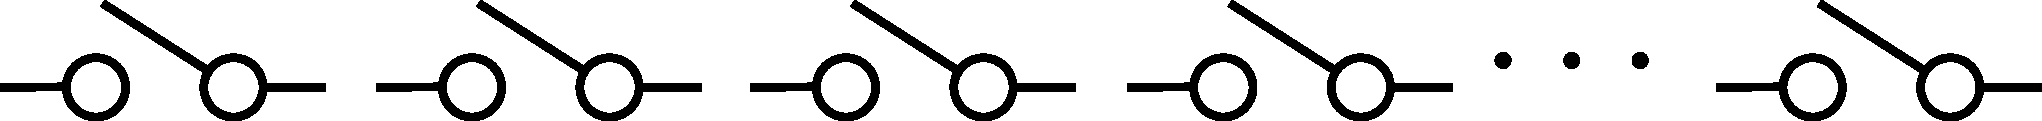
\includegraphics[width=0.75\linewidth]{switches}
	\caption[A configuration of $n$ binary switches where some configuration of the switches is denoted a winning configuration, as an example to illustrate of the search problem Grover's algorithm tries to solve.][-10pt]{A configuration of $n$ binary switches where some configuration of the switches is denoted a winning configuration, as an example to illustrate the search problem Grover's algorithm tries to solve.} 
	\labelFigure{switches}
\end{figure}

\noindent
If you don't have any prior knowledge of the configuration $s$, the best you can do is to simply employ a random guess and check strategy, \ie you might try the combination shown in~\refFigureOnly{switches_comb} and check if the lock opens.

\begin{figure}[h]
    \centering
	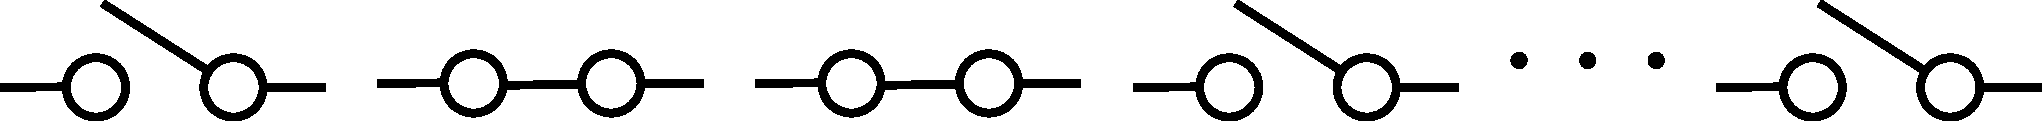
\includegraphics[width=0.75\linewidth]{switches_comb}
	\caption[An example configuration of the $n$ binary switches where two of the switches are in the on state and rest are in the off state.]{An example configuration of the $n$ binary switches where two of the switches are in the on state and rest are in the off state.}
	\labelFigure{switches_comb}
\end{figure}

\noindent
If this is the best you can do, in the worst-case scenario you should expect to try all possible combinations, of which there are $N=2^n$, until you find $s$, thus the worst-case behaviour scales linearly with $N$, $\bigO{N}$. 

\clearpage
\noindent
We can rephrase the above problem more concretely; assume we have the Boolean function $\chi: \{0, 1, \ldots, N-1\} \to \{0,1\}$ such that

\begin{align}
\labelEquation{check_function}
\chi(x) =
	\begin{dcases}
		1 & x=s \\
		0 & x\neq s
	\end{dcases},
\end{align}

\noindent 
for some unknown $s$. We refer to $s$ as a target element. The above problem can be phrased as finding the unknown $s$ by querying the above Boolean function, with some input $x$ and check if $\chi(x) = 1$.

\bigskip
\noindent
On a quantum computer, we can do slightly better than $\bigO{N}$ for the above. We assume here that the size of the search problem is a power of $2$, $N=2^n$ for $n \in \mathbb{N}$. We can thus realize the entire search space for a particular $N$ on $n=\log{(N)}$ qubits~\footnote{All logarithms $\log(\cdot)$ are taken base $2$ unless state otherwise. $\ln(\cdot)$ is reserved for $\log_{e}$}. One of the first clever tricks is to represent the effect of the Boolean function $\chi$ to indicate whether a particular input is a target element as a unitary transformation $U_{\chi}$, which acts on basis states $\ket{x}$ like so,

\begin{align}
U_{\chi}: \ket{x} \to (-1)^{\chi(x)} \ket{x}.
\end{align}

\noindent
Observe for all $x \neq s$, the above unitary transformation acts trivially on the corresponding basis state $\ket{x}$, and for $x = s$, the corresponding basis state acquires a negative phase; the unitary $U_{\chi}$ is often called a phase oracle. $U_{\chi}$ may be written explicitly as,

\begin{align}
	\labelEquation{phase_oracle}
	U_{\chi} = \mathds{1} - 2\op{s}.
\end{align}

\noindent
The algorithm starts with an $n$-qubit state $\ket{0}^{\otimes n}$ and prepares an equal superposition of all basis states, by applying a Hadamard transformation on each qubit,  $H^{\otimes n}$

\begin{align}
	\labelEquation{equal_superpos}
	\ket{\psi} = H^{\otimes n} \ket{0}^{\otimes n} = \frac{1}{\sqrt{N}}\displaystyle\sum_{x=0}^{N-1}\ket{x}.
\end{align}

\noindent
It is useful to write the above state in a different basis. If there are $t$ target elements (and $N-t$ non-target elements), then define $\ket{x_{\perp}}$ and $\ket{x_{//}}$ as such 

\begin{align}
	\ket{x_{\perp}} &= \frac{1}{\sqrt{N-t}}\displaystyle\sum_{x \neq s}\ket{x}, \nonumber \\ 
	\ket{x_{//}} &= \frac{1}{\sqrt{t}}\displaystyle\sum_{x = s}\ket{x},
\end{align}


\noindent
we can rewrite $\ket{\psi}$ as

\begin{align}
	\labelEquation{sol_basis}
	\ket{\psi} = \frac{\sqrt{N-t}}{\sqrt{N}}\ket{x_{\perp}} + \frac{\sqrt{t}}{\sqrt{N}} \ket{x_{//}},
\end{align}

\noindent
We can further adopt the parametrization

\begin{align}
	\theta &= \arcsine{\sqrt{\frac{t}{N}}}, \nonumber \\
	\cos{(\theta)} &= \sqrt{\frac{N-t}{N}}, \nonumber \\
	\sin{(\theta)} &= \sqrt{\frac{t}{N}},
\end{align}

\noindent
for which we can further rewrite~\refEquationOnly{sol_basis} as

\begin{align}
	\labelEquation{angle_basis}
	\ket{\psi} = \cos{(\theta)}\ket{x_{\perp}} + \sin{(\theta)}\ket{x_{//}}.
\end{align}

\noindent
Applying $U_f$ to the above state yields

\begin{align}
	\labelEquation{oracle_app}
	U_{\chi} \ket{\psi} = \cos(\theta)\ket{x_{\perp}} - \sin{(\theta)}\ket{x_{//}}.
\end{align}

\noindent
Another clever trick in Grover's algorithm is an application of another unitary transformation $D$; defined similarly to~\refEquationOnly{phase_oracle}

\begin{align}
	D &= H^{\otimes n} (2\op{0}^{\otimes n} - \mathds{1}) H^{\otimes n}, \nonumber \\
	D &= 2\op{\psi} - \mathds{1}.
\end{align}

\noindent
The above unitary transformation is often called a global diffuser operator. Expanding $D$ in terms of the basis $\{\ket{x_{\perp}}, \ket{x_{//}}\}$, we get to the expression

\begin{align}
	D &= 2\cos^2{(\theta)} \ket{x_{\perp}}\bra{x_{\perp}}  + 2\sin^2{(\theta)}\ket{x_{//}}\bra{x_{//}} \nonumber \\
	&\quad + \sin{(2\theta)}\ket{x_{\perp}}\bra{x_{//}} + \sin{(2\theta)}\ket{x_{//}}\bra{x_{\perp}} - \mathds{1}.
\end{align}

\noindent
We apply $D$ to~\refEquationOnly{oracle_app}, after trigonometric and algebraic gymnastics we arrive at

\begin{align}
	\labelEquation{so2_mat}
	D U_{\chi} \ket{\psi} &= (\cos{2\theta}\cos{\theta} - \sin{2\theta}\sin{\theta})\ket{x_{\perp}} \nonumber \\
					 &\quad + (\sin{2\theta}\cos{\theta} + \cos{2\theta}\sin{\theta})\ket{x_{//}}, \nonumber  \\
					 &= \cos{3\theta}\ket{x_{\perp}} + \sin{3\theta}\ket{x_{//}}.
\end{align}

\noindent
The full $D U_{\chi}$ has a geometric interpretation; the state $\ket{\psi}$ is a vector in a $2$-dimensional Euclidean space spanned by $\ket{x_{\perp}}$ and $\ket{x_{//}}$, initially angled at $\theta$ with respect to $\ket{x_{\perp}}$. $U_{\chi}$ reflects the vector $\ket{\psi}$ about the $\ket{x_{\perp}}$ axis, \ie $\theta \mapsto - \theta$; the angle between $\ket{\psi}$ and $U_{\chi}\ket{\psi}$ at this point is $2\theta$. $D$ finally reflects $U_{\chi}\ket{\psi}$ about the $\ket{\psi}$ axis; the angle between $\ket{x_{\perp}}$ and $D U_{\chi}\ket{\psi}$ is $3\theta$; see figure below.

\begin{figure}[h]
    \centering
	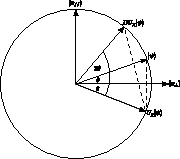
\includegraphics[width=0.60\linewidth]{grover}
	\caption[The geometric interpretation of a single Grover iterate.]{The geometric interpretation of  a single Grover iterate; the uniform superposition state $\ket{\psi}$ starts at an angle $\theta$ with respect to the axis $\ket{x_{\perp}}$, the action of the phase oracle $U_{\chi}$ reflects $\ket{\psi}$ about the axis $\ket{x_{\perp}}$. Likewise, the action of the diffuser operator is to reflect $U_{\chi}\ket{x_{\perp}}$ about the axis $\ket{\psi}$ to get $D U_{\chi}\ket{x_{\perp}}$.}
	\labelFigure{grover_iterate}
\end{figure}

\clearpage
\noindent
Looking at~\refEquationOnly{so2_mat}, we can conveniently write the action of $D U_{\chi}$ on the basis states $\{\ket{x_{\perp}}, \ket{x_{//}}\}$ as 

\begin{align}
	D U_{\chi} = \mqty(\cos{(2\theta)} & -\sin{(2\theta)} \\ \sin{(2\theta)} & \cos{(2\theta)}),
\end{align}

\noindent
that is, $D U_{\chi}$ is an element of the special orthogonal group $SO(2)$, the group of rotations in two dimensions. The unitary operator $G = D U_{\chi}$ is called the global Grover iterate. Rotating by an angle $\theta$ around a point $k$ times is equivalent to a single rotation by an angle $k\theta$. From this, it is easy to see that $k$ applications of $G$ give

\begin{align}
	G^{k} \ket{\psi} = \cos{((2k + 1)\theta)}\ket{x_{\perp}} + \sin{((2k+1)\theta)}\ket{x_{//}}.
\end{align}

\noindent
Another useful visualization aid for gaining intuition about the Grover iterate is look to at its effect at the level of the amplitudes of the state in~\refEquationOnly{equal_superpos}. Consider the case where there is one unique target element; as we have seen the amplitude of the target element $\ket{s}$ acquires a negative phase under the action of unitary operator $U_{\chi}$ while the other amplitudes are left unaltered, hence applying $U_{\chi}$ to~\refEquationOnly{equal_superpos} gives

\begin{align}
	\labelEquation{oracle_action}
	U_{\chi}\ket{\psi} = \frac{1}{\sqrt{N}}\left(-\ket{s} + \displaystyle\sum_{x\neq s} \ket{x}\right).
\end{align}

\noindent
It is not to hard to show that the action of the diffuser operator $D$ on a general $n$-qubit state ~$\ket{\varphi} =\sum_{x=0}^{N-1}\alpha_x\ket{x}$ is given by

\begin{align}
	\labelEquation{diffuser_action}
	D \ket{\varphi} = \displaystyle\sum_{x=0}^{N-1}(2\ev{\alpha} - \alpha_x)\ket{x},
\end{align}

\noindent
where $\ev{\alpha} = \sum_{x=0}^{N-1}\alpha_x / N$ is the average value of the amplitudes~\footnote{The action of the diffuser operator $D$ on the amplitudes of a general state is often called inversion about the average for this reason, since $\alpha_x \to 2\ev{\alpha} - \alpha_x$ for each amplitude $\alpha_x$ associated with a computational basis state $\ket{x}$.}. Hence, when we apply $D$ to $U_{\chi}\ket{\psi}$ in~\refEquationOnly{oracle_action} we obtain the following expression

\begin{align}
	D U_{\chi} \ket{\psi} &= \left(\frac{2(N-2)}{\sqrt{N}N} + \frac{1}{\sqrt{N}}\right)\ket{s} + \left(\frac{2(N-2)}{\sqrt{N}N} - \frac{1}{\sqrt{N}}\right)\displaystyle\sum_{x \neq s}\ket{x}, \nonumber \\
	&= \frac{3N - 4}{\sqrt{N}N}\ket{s} + \frac{N-4}{\sqrt{N}N}\displaystyle\sum_{x \neq s}\ket{x},
\end{align}

\noindent
since $\ev{\alpha} = (N-2)/\sqrt{N}N$; clearly, $3N - 4 > N- 4$. We see that the action of $D U_{\chi}$ is to increase the amplitude associated with the target element $\ket{s}$ while decreasing the amplitudes of the non-target elements (see~\refFigureOnly{amplitude_ampl}). For this reason, the process bears the name amplitude amplification.

\bigskip
\noindent
How many applications $k$ of the global Grover iterate should be applied to guarantee close to unity probability of observing the target element(s) $\ket{x_{//}}$ when we perform an appropriate measurement? Looking at~\refFigureOnly{grover_iterate}, we see that if we do not perform enough iterates we might undershoot and fall short of reaching $\ket{x_{//}}$. More worryingly, we might overshoot past $\ket{x_{//}}$, running the risk of having additional iterations for a clockwise round trip to cycle back close to $\ket{x_{//}}$. 

\clearpage
\begin{figure}[t]
	\subfloat[]
	{
		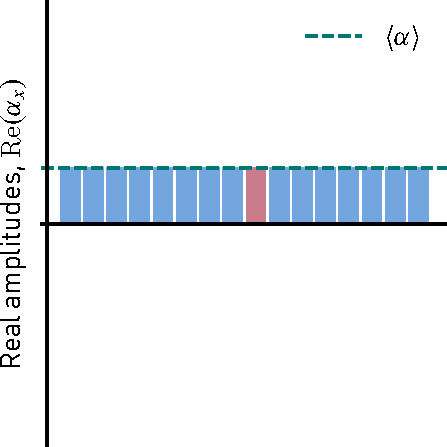
\includegraphics[width=0.33\textwidth]{grover_iter0}
	}
	\subfloat[]
	{
		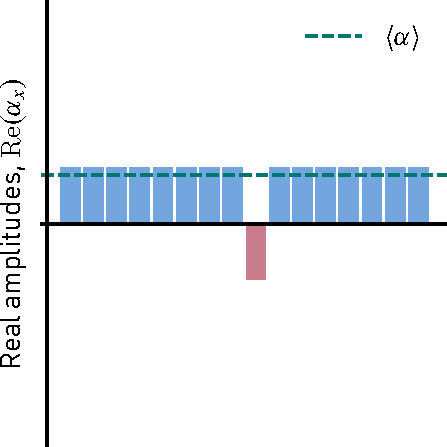
\includegraphics[width=0.33\textwidth]{grover_iter1}
	}
	\subfloat[]
	{
		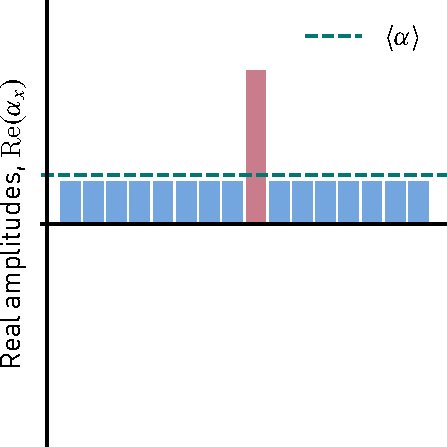
\includegraphics[width=0.33\textwidth]{grover_iter2}
	}
	\caption[The action of a single Grover iterate on the level of the amplitudes for a search space of size ${N=2^4=16}$, where we guaranteed that there is a unique target element.]{The action of a single Grover iterate on the level of the amplitudes for a search space of size ${N=2^4=16}$, when we guaranteed that there is a unique target element. \textbf{(a)} We begin with the uniform superposition state $\ket{\psi}$, the amplitude of the target state is indicated in red while the non-target elements are indicated in blue. \textbf{(b)} After applying the phase oracle, the amplitude of the target element (indicated in red) acquires a relative negative sign. \textbf{(c)} The action of the diffuser operator is to invert all amplitudes about the average amplitude $\ev{\alpha}$. Hence, non-negative amplitudes decrease while negative amplitudes increase; amplifying the amplitude of the target element.}
	\labelFigure{amplitude_ampl}
\end{figure}

\noindent
The probability of measuring $\ket{x_{//}}$ is given by

\begin{align}
	\labelEquation{prob}
	P_k = \abs{\bra{x_{//}}G^{k}\ket{\psi}}^2 = \sin{((2k+1)\theta)}^2.
\end{align}

\noindent
For a particular $\tilde{k}$, we want $P_{\tilde{k}}$ to be close to $1$, that is $\sin{((2\tilde{k}+1)\theta)}^2 \simeq 1$. From elementary trigonometry, we know that $\sin{(\phi)} = 1$ if $\phi = \pi/2$, then it must be that $(2\tilde{k}+1)\theta=\pi/2$, giving $\tilde{k} = \pi/4\theta - \frac{1}{2}$. In instances where $\tilde{k}$ is not integer, if we chose the number of iterations $k$ to be the closest integer to $\tilde{k}$, we will still measure $\ket{x_{//}}$ with high probability. If we pick $\tilde{k}$ as $k =  \left\lfloor\pi/4\theta\right\rfloor$, we have a probability of failure that is less than $t/N$~\cite{Boyer_1998}, as shown below 

\begin{align}
	1 - P_k &= 1 - \sin{((2k+1)\theta)}^2 = \cos{((2k + 1)\theta)}^2, \nonumber \\
			&= \cos{[(2k+1)\theta  + (2\tilde{k} +1)\theta - (2\tilde{k}+ 1)\theta]}^2,  \nonumber \\
			&= \cos{[(2\tilde{k} + 1) + (2(k - \tilde{k}))\theta]}^2, \nonumber \\
			&= \cos{(\pi/2 + 2(k - \tilde{k})\theta)}^2, \nonumber \\
			&= \sin{(2(k - \tilde{k})\theta)}^2, \nonumber \\
			&\leq \sin{(\theta)}^2 = \frac{t}{N},
\end{align}

\noindent
here we used $\abs{k - \tilde{k}} \leq 1/2$ and $(2\tilde{k} + 1)\theta = \pi/2$. The asymptotic behaviour of the number of global Grover iterates $k$ when $t \ll N$ is 

\begin{align}
	k \leq \frac{\pi}{4\theta} = \frac{\pi}{4\arcsine{\sqrt{\frac{t}{N}}}} \leq \frac{\pi}{4}\sqrt{\frac{N}{t}},
\end{align}

\noindent
since $\sqrt{t/N} = \arcsine{(\phi)} \geq \phi$. Hence, the algorithm asymptotically requires $\bigO{\sqrt{N/t}}$ iterations to achieve a probability of success close to one. It is clear that for a given $\theta$,~\refEquationOnly{prob} does not scale linearly with number of iterations $k$ in reaching its maximum value. Noticing this behaviour, Refs.~\cite{Boyer_1998,Gingrich_2000} suggest that if we seek to be frugal in the number of global Grover iterates (steps) --- which is often an overriding imperative in practical considerations particularly for \acs{NISQ} processors with short coherence times --- then we may stop short of $\left\lfloor \pi/4\theta \right\rfloor$ and still find the target element(s) with reasonably high probability. How do we decide when to stop in such a scenario? 

\clearpage
\noindent
The expected number of times we will have to repeat the algorithm until we find a target element, if we stop it every time after $m$ iterations and restart in case of failure is

\begin{align}
	\mathbb{E}[X] &= \displaystyle\sum_{j=1}^{\infty}(m j) P_m(1 - P_m)^{j-1},  \nonumber \\
					  &= \displaystyle\sum_{j=1}^{\infty} (m j) \sin{((2m + 1)\theta)}^2 \cos{((2m + 1)\theta)}^{(2j - 2)}, \nonumber \\
					  &= m\tan{((2m+1)\theta)}^2 \displaystyle\sum_{j=1}^{\infty}j\cos{((2m+1)\theta)}^{2j}, \\
					  &= \frac{m}{\sin{((2m+1)\theta)}^2} = \frac{m}{P_m}, \nonumber \\
					  &= \frac{2m}{1 - \cos{(2(2m + 1)\theta)}}.
\end{align}

\noindent
Here we used $\sum_{j}^{\infty} j\cos{(\phi)}^{2j} = \cot{(\phi)}^2 \cosecant{(\phi)}^2$, and $ \sin{(\phi)}^2 = 1/2(1 - \cos{(2\phi)})$. Taking the derivative of the above expression with respect to $m$ and setting it to zero, we get an expression for $m$ that minimizes the above expression. In the asymptotic limit $t \ll N$, the above expression is minimized when $4m\theta = \tan{(2 m\theta)}$, numerically giving $4 m\theta \approx  2.33112$. This gives the number of iterations as $m \approx 0.58278 \sqrt{N/t}$, and the probability of finding a target element as $P_m = \sin{((2m+1)\theta)}^2 \approx \sin{(2m\theta)}^2 \approx 0.84458$ and $\mathbb{E}[X] \approx 0.69003/\theta \approx 0.8785 \pi/4\theta < \pi/4\theta$.

\bigskip
\noindent
Grover's algorithm has been proved to be asymptotically optimal (no quantum algorithm can achieve the same success with a fewer number of steps) in the number of search queries (iterates)~\cite{Bennett_1997,Boyer_1998,Grover_1998}, with proofs of this kind finally culminating in Ref.~\cite{Zalka_1999}, which shows that the algorithm is not only asymptotically but exactly optimal in the number of search queries. For the sake of brevity, we omit the proofs here and refer the interested reader to the aforementioned references. 

\bigskip
\noindent
A seemingly problematic scenario may arise when we are interested in finding multiple target elements, and we are oblivious to how many are there. That is, we don't know the value of $t$, hence $\theta$. In such a scenario, there is seemingly no way to know how many global Grover iterates we should apply to maximize the probability of finding a target element, $P_k = \sin{((2k+1)\theta)}^2$. Fortunately, it turns out it is still possible to preserve the asymptotic optimality of the algorithm, $\bigO{\sqrt{N}{t}}$, if we adopt a method that continuously tries and updates informed guesses for $k$, and restarting the algorithm in case of failure, with the assumption that $t$ is bounded above by $\left\lceil  3N/4 \right\rceil$, the interested reader may refer to Ref.~\cite{Boyer_1998} for more details. We show the schematic circuit diagram of Grover's algorithm in~\refFigureOnly{grover_schematic}, and conclude this subsection by summarizing the steps of Grover's quantum search algorithm when the number of target elements $t$ is known.

\begin{enumerate}
\item \emph{Initialization}\newline
Prepare $\ket{0}^{\otimes n}$ and apply $H^{\otimes n}$ on all the qubits, creating a uniform superposition of $N=2^n$ basis states:

\begin{align*}
    \ket{0}^{\otimes n} \to \frac{1}{\sqrt{N}}\displaystyle\sum_{x=0}^{N-1} \ket{x}.
\end{align*}

\item \emph{Global Grover iterates}\newline
Apply the global Grover iterates $k$ times, where $k=\left\lfloor \sqrt{N/t}\pi/4  \right\rfloor$ for close to unity success and $k=0.58278\sqrt{N/t}$ for a success probability of $\simeq 0.8446$:
\begin{align*}
	\frac{1}{\sqrt{N}}\displaystyle\sum_{x=0}^{N-1} \ket{x} \to \frac{1}{\sqrt{N}}\displaystyle\sum_{x=0}^{N-1} G^{k}\ket{x}.
\end{align*}

\item \emph{Measurements}\newline
    Measure all qubits in the computational basis, yielding a target element in with high probability if $k=\left\lfloor\sqrt{N/t}\pi/4  \right\rfloor$. In case of failure for $k=0.58278\sqrt{N/t}$, go back to step 1; the average number of times we will have to repeat the algorithm is at least $\simeq 0.8785\sqrt{N/t}\pi/4$ times before success.

\end{enumerate}

\begin{figure}[h]
	\centering
	\resizebox{0.65\textwidth}{!}{%
	\begin{tikzpicture}
	\begin{yquant}[register/separation=4mm]
		qubit {$\ket{x_{\idx}} = \ket0$} j[2];
		nobit ellipsis;
		qubit {$\ket{x_{n}} = \ket{0}$} jn;
		h j;
		vdots ellipsis;
		h jn;

		[this subcircuit box style={draw, dashed, inner ysep=6pt, label=above:Repeat $\bigO{\sqrt{N/t}}$ times}]
		subcircuit {
			qubit {} j[2];
			nobit ellipsis;
			qubit {} jn;

			[x radius=0.3cm]
			box {$U_{\chi}$} (j-jn);
			h j;
			h jn;
			[x radius=1cm]
			box {$2\op{0}^{\otimes n} - \mathds{1}$} (j-jn);
			h j;
			h jn;
		} (j, jn, ellipsis);
		measure j;
		vdots ellipsis;
		measure jn;
	\end{yquant}
	\end{tikzpicture}
	}
	\caption[A schematic circuit diagram of Grover's algorithm.][-20pt]{A schematic circuit diagram of Grover's algorithm; which begins with all $n$ qubits in the state $\ket{0}$, after which a Hadamard gate $H$ is applied to all qubits to create a uniform superposition of $2^n$ basis states. Grover iterates, with each consisting of a phase oracle and diffuser operators are repeated $\bigO{\sqrt{N}}$. Measuring the qubits in the computational basis, with high probability we obtain the outcome corresponding to the target element.} 
	\labelFigure{grover_schematic}
\end{figure}



\subsection{Partial search quantum algorithm}
\labelSection{C2_partial_search_quantum_algorithm}
The partial search quantum algorithm due to Grover and Radhakrishnan~\cite{Grover_2005} offers another way we might trade accuracy for fewer elementary operations. Rather than searching for a target element\footnote{In the case where we are assured this is one unique target element,~\ie ${t=1}$.}, the partial search quantum algorithm instead partitions the search space into $K=2^{n-m}$ blocks of size $b=2^m$,~\ie $N=bK=2^n$, and searches on the level of blocks, that is, it seeks find the block to which a target element belongs rather than the target element itself. Intuitively, this can be understood as performing the canonical quantum search algorithm on the first $(n-m)$ bits of the target element $s$. The analysis proceeds in a similar way to the canonical quantum search of the previous section; we begin with $\ket{0}^{\otimes n}$ and prepare a uniform superposition, by applying Hadamard gates to every qubit, preparing the state in~\refEquationOnly{equal_superpos}. In the case of a single and unique target element\footnote{The algorithm has been generalized to accommodate multiple target elements across the blocks~\cite{Choi_2007,Zhang_2018}. In such a scenario optimality is achieved when the target elements are evenly distributed across the blocks~\cite{Zhang_2018}. We do not consider such cases here. The interested reader may refer to the aforementioned references.}, we introduce the basis

\begin{align}
	\ket{s} &= \ket{s_1} \otimes \ket{s_2}, \nonumber \\
	\ket{ns} &= \frac{1}{\sqrt{b-1}}\displaystyle\sum_{x \neq x_1} \ket{x_1} \otimes \ket{x}, \nonumber \\
	\ket{u} &= \frac{1}{\sqrt{N-b}}(\sqrt{N}\ket{\psi} - \ket{s} - \sqrt{b-1}\ket{ns}),
\end{align}

\noindent
here $\ket{s}$ is the target element, bipartitioned into a product state of $\ket{s_1} \text{ and } \ket{s_2}$, where we seek to find $\ket{s_1}$, $\ket{ns}$ is the normalized sum of all non-target elements in the block containing the target element$\ket{s}$, $\ket{u}$ is the normalized sum of all the elements belong to blocks not containing $\ket{s}$, and $\ket{\psi}$ is the uniform superposition in~\refEquationOnly{equal_superpos}.  

\clearpage
In this new basis, we can write~\refEquationOnly{equal_superpos} as

\begin{align}
	\ket{\psi} = \frac{1}{\sqrt{N}}\ket{s} + \frac{\sqrt{b-1}}{\sqrt{N}}\ket{ns} + \frac{\sqrt{N-b}}{\sqrt{N}}\ket{u}.
\end{align}

We adopt the following parametrization

\begin{align}
	\sin{(\theta)} &= \frac{1}{\sqrt{K}}, \nonumber \\
	\cos{(\theta)} &= \frac{\sqrt{K-1}}{\sqrt{K}}, \nonumber \\
	\sin{(\phi)}   &= \frac{1}{\sqrt{b}}, \nonumber \\
	\cos{(\phi)}   &= \frac{\sqrt{b-1}}{\sqrt{b}},
\end{align}

\noindent
and arrive at

\begin{align}
	\labelEquation{spherical_vec}
	\ket{\psi} = \sin{(\theta)}\sin{(\phi)}\ket{s} + \cos{(\phi)}\sin{(\theta)}\ket{ns} + \cos{(\theta)}\ket{u}.
\end{align}

\noindent
We see that $\ket{\psi}$ may be taken to be a vector in a spherical coordinate system with coordinates ($1$ (radius), $\theta$ (inclination), $\phi$ (azimuth)) where the $x$-axis is defined by $\ket{ns}$, $y$-axis by $\ket{s}$ and the $z$-axis by $\ket{u}$. We proceed in a similar fashion and apply the phase oracle $U_{\chi}$ to~\refEquationOnly{spherical_vec}, giving the amplitude of the target element $\ket{s}$ a negative sign. The crucial distinction between the canonical and partial search quantum algorithm is the introduction of a local diffuser operator $D_{n,m}$, which acts in the same way the global diffuser operator $D$ does but on a subspace of $m$ qubits rather than all the qubits, $m < n$. That is,

\begin{align}
	D_{n,m} = \mathds{1}_{2^{n-m}} \otimes (2\op{\phi} - \mathds{1}_{2^m}),
\end{align}

\noindent
where $\ket{\phi} = H^{\otimes m} \ket{0}^{\otimes m}$ is a uniform superposition of $m$ qubits in such a subspace. The unitary operator $D_{n,m}$ has a similar effect on the amplitudes as $D$ does, that is, it inverts about the average in each block simultaneously. The unitary operator $G_{n,m} = D_{n,m}U_{\chi}$ is called the local Grover iterate\footnote{From now on, we will denote to global Grover iterates with a with a single subscript $G_{n}$, instead of $G_{n,n}$. Similarly, we will indicated a global diffuser operator $D_{n}$ instead of $D_{n,n}$.}; we can similarly trace its effects on~\refEquationOnly{spherical_vec} as before by looking at the evolution of the amplitudes after each step, as shown in~\refFigureOnly{amplitude_localampl}.

\bigskip
\noindent
A feature worth noting is that for some choice of the block size $b$, the local Grover iterate can amplify the amplitude of the target element to a moderately high value relative to the rest of the amplitudes. Grover and Radhakrishnan noticed this too, and in Ref.~\cite{Grover_2005} suggested that we can use local Grover iterates in conjunction with global Grover iterates to guarantee a high probability of measuring the target element. 

\bigskip
\noindent
The order in which global and local Grover iterates are applied is important, since the two operators share non-trivial commutation relations,~\refFigureOnly{iterate_order} shows the amplitudes after applying two local Grover iterates $G_{n,m}$ and one global Grover iterate $G_{n}$ in different orders. Ref.~\cite{Grover_2005} proves that it is possible to guarantee a high probability of measuring the target if $l_1$ sequences of the global Grover iterates $G_n$ are applied first followed by $l_2$ sequences of local Grover iterates $G_{n,m}$, and lastly a single global Grover iterate $G_n$, that is, $G_n G_{n,m}^{l_2}G_{n}^{l_1}$.

\clearpage

\begin{figure}[t!]
	\subfloat[\labelFigure{grover_localiter0}]
	{
		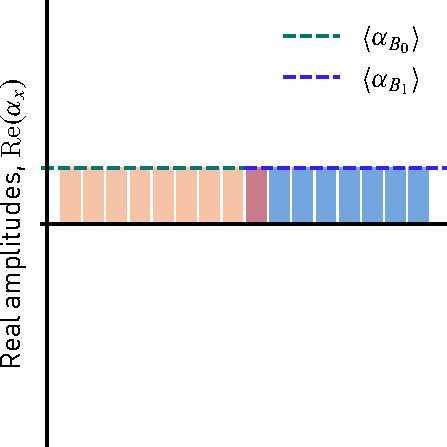
\includegraphics[width=0.33\textwidth]{grover_localiter0}
	}
	\subfloat[\labelFigure{grover_localiter1}]
	{
		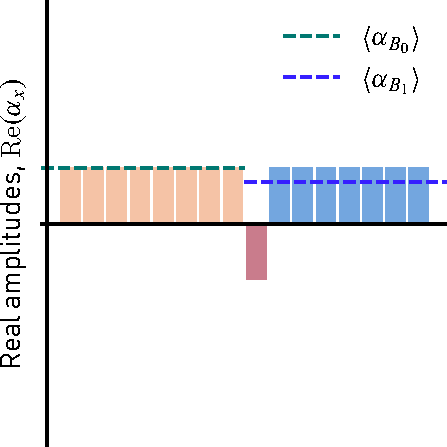
\includegraphics[width=0.33\textwidth]{grover_localiter1}
	}
	\subfloat[\labelFigure{grover_localiter2}]
	{
		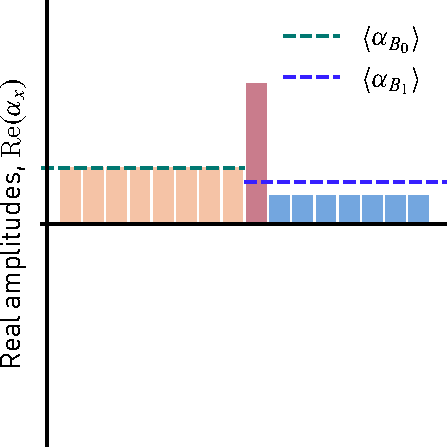
\includegraphics[width=0.33\textwidth]{grover_localiter2}
	}
	\caption[The action of a single local Grover iterate on the level of the amplitudes for a search space of size ${N=2^4}$ and a block size ${b=2^{3}}$, which divides the search into ${K=2}$ blocks.]{The action of a single local Grover iterate on the level of the amplitudes for a search space of size ${N=2^4}$ and a block size ${b=2^{3}}$, which divides the search into ${K=2}$ blocks. $\ev{\alpha_{B_0}}$ and $\ev{\alpha_{B_1}}$ represent the block average for each block. \textbf{(a)} We begin with the uniform superposition state $\ket{\psi}$, the amplitude of target element is indicated in red and the rest of amplitudes in the target block is indicated in blue, while all the amplitudes in the non-target block indicated in orange. \textbf{(b)} After applying the phase oracle the amplitude of the target state acquires a relative minus sign. \textbf{(c)} The action of local diffuser operator $D_{4,3}$ is to invert the amplitudes in each block about the block's average amplitude, thus non-negative amplitudes decrease while negative amplitudes increase in each block; amplifying the amplitude of the target element.}
	\labelFigure{amplitude_localampl}
\end{figure}

\noindent
They further show that the number of iterates (both local and global) for large values of $K$ scales like $~\pi/4\sqrt{N} - c\sqrt{b}$ for a positive constant $c$. Refs.~\cite{Korepin_2005,Korepin_2006,Choi_2006,Korepin_2006a,Korepin_2006b} study various sequence and application orders of $G_{n,m}$ and $G_{n}$ with the aim of reducing the constant $c$, culminating in Ref.~\cite{Korepin_2006} showing that sequences of the kind $G_{n}G_{n,m}^{l_1}G_{n}^{l_2}$ are optimal among different classes of sequences. The values of $l_1,l_2$ can be found by minimizing $S = l_1 + l_2 + 1 \simeq \pi / 4 \sqrt{N} - c \sqrt{b}$ for a certain probability threshold value and number of blocks $K$. Ref.~\cite{Korepin_2005} adopts the parametrization $l_1 = \pi / 4 \sqrt{N} - \eta_K\sqrt{b}$ and $l_2 = \alpha_K\sqrt{b}$ and numerically minimizes $c = (\alpha_K - \eta_K)$; ~\refTableOnly{numeric_vals} shows some values for $\alpha_K$ and $\eta_K$ from the aforementioned reference. The quantum partial search with this sequence of local and global is called the \gls{GRK} algorithm. ~\refEquationOnly{spherical_vec} is suggestive that the partial quantum search algorithm has a similar geometric interpretation as the canonical quantum search. Indeed, $G_{\text{GRK}} = G_{n}G_{n,m}^{l_1}G_{n}^{l_2}$ is an element of the orthogonal group $O(3)$~\cite{Korepin_2006b}.

\begin{figure}[h]
	\subfloat[\labelFigure{grover_order0}]
	{
		% DD DD D
		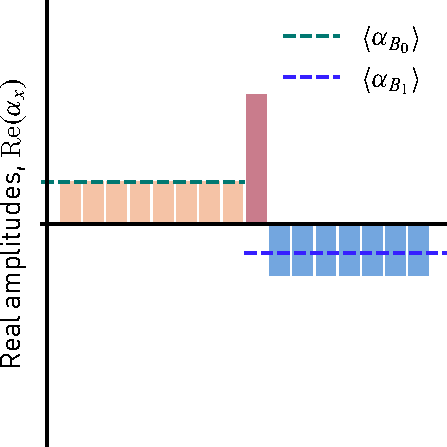
\includegraphics[width=0.33\textwidth]{grover_order0}
	}
	\subfloat[\labelFigure{grover_order1}]
	{
		% DD D DD
		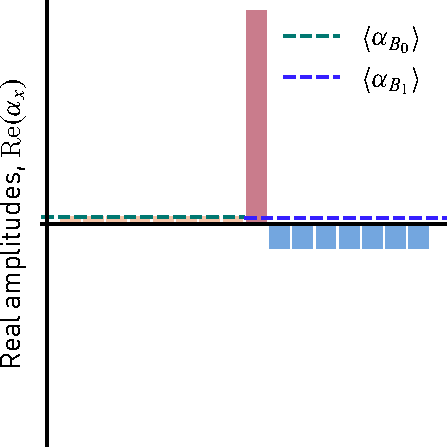
\includegraphics[width=0.33\textwidth]{grover_order1}
	}
	\subfloat[\labelFigure{grover_order2}]
	{
		%% D DD DD
		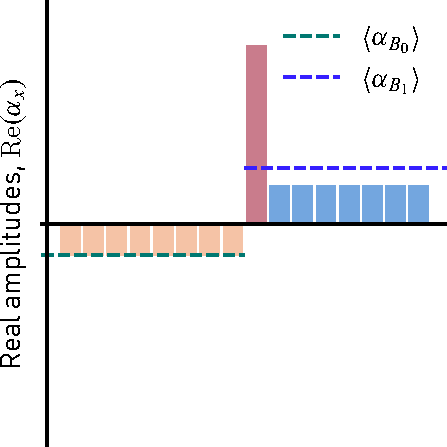
\includegraphics[width=0.33\textwidth]{grover_order2}
	}
	\caption[The actions of different ordering of a global and two local Grover iterates on the level of the amplitudes for ${N=2^4}$, ${b=2^3}$, and ${K=2}$. $\ev{\alpha_{B_0}}$ and $\ev{\alpha_{B_1}}$ represent the block average for each block.]{The actions of different application order of a global and two local Grover iterates on the level of the amplitudes for ${N=2^4}$, ${b=2^3}$, and ${K=2}$. $\ev{\alpha_{B_0}}$ and $\ev{\alpha_{B_1}}$ represent the block average for each block. Action of the application order \textbf{(a)} $G_{4,3}G_{4,3}G_{4}$, \textbf{(b)} $G_{4,3}G_{4}G_{4,3}$, and \textbf{(c)} $G_{4}G_{4,3}G_{4,3}$. The order of operators is important since the local and global Grover operators have non-trivial commutation relations, in all three scenarios we end up with different probabilities for the target element.}
	\labelFigure{iterate_order}
\end{figure}

\bigskip
\noindent
We summarize the \acs{GRK} algorithm to conclude the subsection and show its schematic in~\refFigureOnly{grk_schematic}.

\begin{table}[h]
		\centering
		\caption[Numeric values for $\alpha_K$ and $\eta_K$ for different values of the number of blocks $K$ for the \acs{GRK} algorithm adopted from Korepin et. al]{Numeric values for $\alpha_K$ and $\eta_K$ for different values of the number of blocks $K$ for the \acs{GRK} algorithm, adopted from Ref.~\protect\cite{Korepin_2005}.}
		\labelTable{numeric_vals}
		\begin{tabular}{lll}
			\toprule
			$K$ & $\alpha_K$ & $\eta_K$ \\
			\toprule
			$2$  & $0.7854$     & $1.1107$ \\
			$3$  & $0.65906$    & $0.9961$ \\ 
			$4$  & $0.6155$     & $0.9553$ \\
			$5$  & $0.6155$     & $0.9341$ \\
			$\infty$ & $0.5236$ & $0.866$  \\
			\toprule
		\end{tabular}
\end{table}

\clearpage

\begin{figure}[t!]
	\centering
	\resizebox{1.0\textwidth}{!}{%
	\begin{tikzpicture}
	\begin{yquant}[register/separation=4mm]
		qubit {$\ket{x_{\idx}} = \ket0$} j[2];
		nobit ellipsis;
		qubit {$\ket{x_{m}} = \ket{0}$} jnm;
		nobit ellipsis2;
		qubit {$\ket{x_{n}} = \ket{0}$} jn;
		h j;
		vdots ellipsis;
		h jnm;
		vdots ellipsis2;
		h jn;

		[this subcircuit box style={draw, dashed, inner ysep=6pt, label=above:Repeat $l_1 \simeq \pi / 4 \sqrt{N} - \eta_K\sqrt{b}$ times}]
		subcircuit {
			qubit {} j[2];
			nobit ellipsis;
			qubit {} jnm;
			nobit ellipsis2;
			qubit {} jn;

			[x radius=0.3cm]
			box {$U_{\chi}$} (j-jn);
			h j;
			h jnm;
			h jn;
			[x radius=0.5cm]
			box {$2\op{0}^{\otimes n} - \mathds{1}$} (j-jn);
			h j;
			h jnm;
			h jn;
		} (j, jnm, jn, ellipsis, ellipsis2);

		[this subcircuit box style={draw, dashed, inner ysep=6pt, label=above:Repeat $l_2 \simeq \alpha_K\sqrt{b}$ times}]
		subcircuit {
			qubit {} j[2];
			nobit ellipsis;
			qubit {} jnm;
			nobit ellipsis2;
			qubit {} jn;

			[x radius=0.3cm]
			box {$U_{\chi}$} (j-jn);
			h j;
			h jnm;
			[x radius=0.5cm]
			box {$2\op{0}^{\otimes m} - \mathds{1}_{2^m}$} (j-jnm);
			h j;
			h jnm;
		} (j, jnm, jn, ellipsis, ellipsis2);

		[x radius=0.3cm]
		box {$U_{\chi}$} (j-jn);
		h j;
		h jnm;
		h jn;
		[x radius=0.5cm]
		box {$2\op{0}^{\otimes n} - \mathds{1}$} (j-jn);
		h j;
		h jnm;
		h jn;


		measure j;
		vdots ellipsis;
		measure jnm,jn;
	\end{yquant}
	\end{tikzpicture}
	}
	\caption[A schematic circuit diagram of the \acs{GRK} algorithm.]{A schematic circuit diagram of the \acs{GRK} algorithm; which begins with all $n$ qubits in the state $\ket{0}$, after which a Hadamard gate $H$ is applied to all qubits to create a uniform superposition of $2^n$ basis states. A sequence of $l_1$ global Grover operators, followed by a sequence of $l_2$ local Grover iterates, and lastly a single global Grover operator is applied to the uniform superposition. Measuring in the computational basis, the target element will be found with high probability.}
	\labelFigure{grk_schematic}
\end{figure}


\bigskip
\begin{enumerate}
\item \emph{Initialization}\newline
Prepare $\ket{0}^{\otimes n}$ and apply $H^{\otimes n}$ on all the qubits, creating a uniform superposition of $N=2^n$ basis states:
\begin{align*}
    \ket{0}^{\otimes n} \to \frac{1}{\sqrt{N}}\displaystyle\sum_{x=0}^{N-1} \ket{x}
\end{align*}

\item \emph{Global Grover iterates}\newline
Apply the global Grover iterates $l_1 \simeq \pi / 4 \sqrt{N} - \eta_K\sqrt{b}$ times:
\begin{align*}
	\frac{1}{\sqrt{N}}\displaystyle\sum_{x=0}^{N-1} \ket{x} \to \frac{1}{\sqrt{N}}\displaystyle\sum_{x=0}^{N-1} G_{n}^{l_1}\ket{x}
\end{align*}

\item \emph{Local Grover iterates}\newline
Apply local Grover iterates $l_2 \simeq \alpha_K\sqrt{b}$ times: 

\begin{align*}
	\frac{1}{\sqrt{N}}\displaystyle\sum_{x=0}^{N-1} G_{n}^{l_1}\ket{x} \to \frac{1}{\sqrt{N}}\displaystyle\sum_{x=0}^{N-1} G_{n,m}^{l_2}G_{n}^{l_1}\ket{x}
\end{align*}

\item \emph{Single global Grover iterate}\newline
Apply a single global Grover iterate: 

\begin{align*}
	\frac{1}{\sqrt{N}}\displaystyle\sum_{x=0}^{N-1} G_{n,m}^{l_2}G_{n}^{l_1}\ket{x} \to \frac{1}{\sqrt{N}}\displaystyle\sum_{x=0}^{N-1} G_{n} G_{n,m}^{l_2}G_{n}^{l_1}\ket{x}
\end{align*}


\item \emph{Measurements}\newline
    Measure all qubits in the computational basis yielding a target element with high probability. In case of failure, go back to step 1.
\end{enumerate}

\section{Survey of recent results relating to NISQ processors}
\labelSection{C2_survey_of_recent_results_on_nisq_processors}
As we have seen in sections ~\refSectionOnly{C2_canonical_construction_of_grovers_algorithm} and ~\refSectionOnly{C2_partial_search_quantum_algorithm}, both the canonical and partial quantum search algorithms in various scenarios have been proven to be optimal in the number of steps they undertake to solve the search problem. However, as I briefly alluded to in the opening of this chapter, in physical implementations (emphasis on \acs{NISQ} processors) of any quantum algorithm, each of these steps are broken down into intermediary subroutines and further into physically realizable atomic operations in the universal gate set of a particular physical implementation. 

\bigskip
\noindent
For physical realizations of quantum search algorithms, the Grover iterates constitute the most resource intensive parts of the algorithm in terms of such atomic operations. The phase oracle $U_{\chi}$ in the Grover iterate is equivalent to an $n$-qubit controlled-$Z$ gate (modulo single qubit gates). Suppose our unique target element is the computational basis state $\ket{b_0b_1b_2\cdots b_{n-1}}$, then following circuit composed of Pauli $X$ gate and $n$-qubit controlled-$Z$, $C^{n-1}[Z]$ gates, implements a phase oracle $U_{\chi}$ that gives the state $\ket{b_0b_1b_2 \cdots b_{n-1}}$ a relative negative amplitude~\footnote[][-50pt]{For $n=2$, it is equivalent to a controlled-$Z$ and for $n=3$ it is equivalent to a controlled-controlled-$Z$ gate.}.

\begin{figure}[h]
    \centering
	\begin{tikzpicture}
		\begin{yquant}[register/separation=2mm]
			qubit {$b_{\idx}$} q[2];
			[name=wave, register/minimum height=8mm]
			nobit wave;
			qubit {$b_{n-2}$} qm;
			qubit {$b_{n-1}$} qn;
			box {$X^{\neg b_0}$} q[0];
			box {$X^{\neg b_1}$} q[1];
			vdots wave;
			box {$X^{\neg b_{n-2}}$} qm;
			box {$X^{\neg b_{n-1}}$} qn;
			box {$Z$} qn | q[0],q[1], qm;
			box {$X^{\neg b_0}$} q[0];
			box {$X^{\neg b_1}$} q[1];
			vdots wave;
			box {$X^{\neg b_{n-2}}$} qm;
			box {$X^{\neg b_{n-1}}$} qn;
		\end{yquant}
	\end{tikzpicture}
    \caption[A circuit diagram that realizes a general phase oracle in Grover's algorithm.]{A circuit diagram that realizes a general phase oracle in Grover's algorithm; the circuit maps ${\ket{b_0b_1b_2 \cdots b_{n-1}} \to -\ket{b_0b_1b_2 \cdots b_{n-1}}}$, where $(X_a)^{b_a}$ applies a Pauli $X$ gate to qubit a if $b_a=1$ and applies the identity if $b_0$. $Z$ denotes the Pauli $Z$ gate}
	\labelFigure{phase_oracle_circ}
\end{figure}

\noindent
where $\neg 0 = 1$ and $\neg 1 = 0$.  The diffuser operator $G_n$ is implemented similarly

\begin{figure}[h]
    \centering
	\begin{tikzpicture}
		\begin{yquant}[register/separation=2mm]
			qubit {$b_{\idx}$} q[2];
			[name=wave, register/minimum height=8mm]
			nobit wave;
			qubit {$b_{n-2}$} qm;
			qubit {$b_{n-1}$} qn;
			h q;
			box {$X$} q[0];
			box {$X$} q[1];
			vdots wave;
			h qm;
			h qn;
			box {$X$} qm;
			box {$X$} qn;
			box {$Z$} qn | q[0],q[1], qm;
			box {$X$} q[0];
			box {$X$} q[1];
			h q;
			vdots wave;
			box {$X$} qm;
			box {$X$} qn;
			h qm;
			h qn;
		\end{yquant}
	\end{tikzpicture}
    \caption[A circuit diagram that realizes a global diffuser operator in Grover's algorithm.]{A circuit diagram that realizes a global diffuser operator in Grover's algorithm, where $X, Z, H$ are the Pauli $X,Z$ and $H$ is the Hadamard gate respectively.}
	\labelFigure{diffuser_circ}
\end{figure}

\noindent
 As we have seen, these two operators (the Grover iterate $D_{n}U_{\chi}$) must be repeated several times to guarantee some threshold for the probability of success. For \acs{NISQ} processors, the $n$-qubit controlled-$Z$ gate for more than two qubits is not an atomic operation. The $n$-qubit controlled-$Z$ gate is equivalent to a generalized $n$-qubit Toffoli gate, $C^{n-1}[X]$, by applying a Hadamard gate $H$ to the target qubit just before and after the gate (\ie $HZH = X$). The generalized $n$-qubit Toffoli gate itself is also not an atomic operation on \acs{NISQ} processors, but instead decomposed into atomic operations (controlled-NOT and single qubits). The two-qubit gate such as the controlled-NOT gate are physically realized through two-qubit interactions that induce conditional dependence of the state of one qubit to the other, for instance a cross-resonance interaction for superconducting qubits~\cite{Kjaergaard_2020} and Mølmer-Sørensen interaction for trapped ions qubits~\cite{Bruzewicz_2019}. The commonality across \acs{NISQ} architectures is that such two-qubit interactions are non-trivial, making them experimentally expensive and much more prone to errors than single-qubit gates. Hence, for reasons motivated by practicality, the analysis of circuit complexity is done usually in terms of the two-qubit gate count in a circuit.

 \bigskip
 \noindent
 For $n=3$, the controlled-controlled-$Z$ (hence the controlled-controlled-NOT gate) gate cannot be implemented with less than five two-qubit gates~\cite{Yu_2013}; the traditional three-qubit decomposition shown in~\refFigureOnly{control_control_z}, uses six controlled-NOT and seven $T/T^{\dagger}$ gates, has shown to be optimal in terms of controlled-NOT count~\cite{Shende_2008}. However, for $n\geq4$ the exact controlled-NOT count of its decomposition without the use auxiliary of qubits is not known~\cite{Shende_2008}. He~\etal~\cite{He_2017} have shown that if a single auxiliary qubit is provided $24n − 72$ controlled-NOT gates suffice.

\clearpage
\begin{figure}[t!]
	\centering
	\begin{tikzpicture}
		\begin{yquantgroup}[register/separation=2mm]
			\registers{
				qubit {} q[3];
			}
			\circuit{
				box {$Z$} q[2] | q[0-1];
			}

			\equals 

			\circuit{
				cnot q[2] | q[1];
				box {$T^\dagger$} q[2];
				cnot q[2] | q[0];
				box {$T$} q[2];
				cnot q[2] | q[1];
				box {$T^\dagger$} q[2];
				cnot q[2] | q[0];
				box {$T$} q[2];
				box {$T$} q[1];
				cnot q[1] | q[0];
				box {$T^\dagger$} q[1];
				box {$T$} q[0];
				cnot q[1] | q[0];
			}


		\end{yquantgroup}
	\end{tikzpicture}
	\caption[A circuit diagram showing the decomposition of a controlled-controlled-$Z$ gate in terms of elementary gates.]{A circuit diagram showing the decomposition of a controlled-controlled-$Z$ gate in terms of elementary gates; six controlled-NOT and seven $T/T^{\dagger}$ gates.}
	\labelFigure{control_control_z}
\end{figure}

\noindent
Additionally, they show that if $n-1$ auxiliary qubits are provided, then $4n − 7$ controlled-NOT gates suffice. With such a decomposition it is possible to trade for a great reduction of controlled-NOT gates at the expensive of using more qubits. The unavoidable consequence for physical implementations is that, it becomes much harder to maintain quantum coherence as the relevant Hilbert space is much larger (from $2^n$ to $2^{2n -1}$ possible states). Furthermore, \acs{NISQ} processors have limited connectivity among the qubits on the physical device hence multi-qubit gates cannot be performed directly on qubits that are not directly connected, and instead must be done by way of appropriate SWAP gates; a single SWAP gate costs three controlled-NOT gates, as shown in~\refFigureOnly{swap_gate}

\begin{figure}[h]
    \centering
	\begin{tikzpicture}
		\begin{yquantgroup}[register/separation=8mm]
			\registers{
				qubit {} q[2];
			}

			\circuit{
				swap (q[0, 1]);
			}

			\equals

			\circuit{
				cnot q[1] | q[0];
				cnot q[0] | q[1];
				cnot q[1] | q[0];
			} 
		\end{yquantgroup}
	\end{tikzpicture}
    \caption[A circuit diagram showing the decomposition of a SWAP gate in terms of elementary gates.]{A circuit diagram showing the decomposition of a SWAP gate in terms of elementary gates; three controlled-NOT gates.} 
	\labelFigure{swap_gate}
\end{figure}

\noindent
The theoretical reduction of the controlled-NOT gate count gained by the use of auxiliary qubits in practice may be lost depending on the connectivity of the physical device. Besides, the two-qubit gate count, another way circuit complexity is examined is in terms of its circuit depth. Circuit depth is the number of consecutive parallel operations in a circuit from its input to output. Each such parallel operation can be counted as a single step, and thus circuit depth can be taken to be a good proxy for algorithmic time. Analysis in terms of circuit depth is also motivated by practicality, since \acs{NISQ} processors have short-lived coherence times, over which a computation can remain fully coherent, and thus limited to realizing shallow depth circuits~\cite{Preskill_2018}. The aforementioned decomposition of an $n$-qubit Toffoli due to He~\etal~\cite{He_2017} has a linear depth $\bigO{n}$ and logarithmic depth $\bigO{\log{n}}$ for a single auxiliary qubit and $n-1$ auxiliary qubits, respectively.

\subsection{Depth optimization of the quantum search}
\labelSection{C2_depth_optimization_of_the_quantum_search}
On the account of the limitations of \acs{NISQ} processors,~\ie the short-lived coherence time, limited number of qubits and limited connectivity among qubits, an analysis by Zhang and Korepin~\cite{Zhang_2020} emphasizes the imperative of designing algorithms in such a way that is aware of these limitations. Inspired by the \acs{GRK} algorithm, and these practical considerations, they proposed a modification of the quantum search algorithm that is optimal in circuit depth, not necessarily optimal in the number of steps with respect to achieving some probability threshold. To facilitate this optimization, they define a figure of merit $\alpha$, that is a ratio of the depth of the phase oracle depth and depth of the diffuser operator $D_n$

\begin{align}
	\labelEquation{depth_ratio}
	\alpha = \frac{d(U_{\chi})}{d(D_n)},
\end{align}

\noindent
for single-target oracle implementations of the kind in~\refFigureOnly{phase_oracle_circ} and global diffuser operator of the kind in~\refFigureOnly{diffuser_circ}, since the dominating circuit depth arises from the $n$-qubit controlled-$Z$ gate, it is expected that $\alpha=1$. 

\clearpage
\noindent
Recall that the local diffuser operators $D_{n,m}$ act on a small subspace  $m < n$, thus in theory require fewer elementary operators and have lower depth than the global diffuser operators, at the cost of reducing the success probability\footnote{This is clear from the perspective of~\refFigureOnly{diffuser_circ}, we expect an $m$-qubit controlled-$Z$ gate will decomposed into fewer elementary gates than $n$-qubit controlled-$Z$ gate if $m < n$.}; hence their optimization method is based on the replacement of global diffuser operators with local diffuser operators to minimize the depth of Grover's algorithm, while taking into account the trade-off in the probability of success. Similar to the \acs{GRK} algorithm, they consider a general sequence of local ($G_m$) and global Grover iterate operators ($G_n$) of the form

\begin{align}
	\labelEquation{local_optimal_seq}
	S_{n,m}(\bar{l}) =  G_n^{l_1} G_m^{l_2} \cdots G_n^{l_{q-1}}G_m^{l_q},
\end{align}

\noindent
here $\bar{l} = (l_1, l_2, \ldots, l_q)$ is a tuple of natural numbers, $l_\text{tot} = \sum_{p=1}^{q}l_p$ is the total number of Grover iterates (both local and global). For instance, $S_{n}(l,0)=G_n^l$ is the canonical Grover algorithm. The notational convention is that last number $l_q$ is always the number of local Grover iterate operators, thus in this notation the Grover iterate for the \acs{GRK} is denoted by $S_{n,m}(1,l_2,l_1,0) = G_n^{1}G_m^{l_2}G_n^{l_1}G_m^{0}$. Furthermore, the above notation only considers local Grover iterate operators acting on the same qubit subspace with the same block size $m$. For such a sequence of Grover iterates, the probability of measuring the target element $\ket{s}$ is given by

\begin{align}
	P_{n,m}(\bar{l}) = \abs{\mel{s}{S_{n,m}(\bar{l})H^{\otimes n}}{0}^{\otimes n}}^2.
\end{align}

\noindent
From this, they define the ratio of the expected depth for the Grover iterate sequence $S_{n,m}$ and its probability of success as 

\begin{align}
	\tilde{d}(\alpha) = \frac{d(S_{n,m}(\bar{l}))}{P_{n,m}(\bar{l})},
\end{align}

\noindent
and minimize the above quantity with respect both $m \geq 2$ and the tuple of natural numbers $\bar{l}$.

\begin{align}
	\tilde{d}(\alpha) = \underset{m, \bar{l}}{\text{minimize }}\frac{d(S_{n,m}(\bar{l}))}{P_{n,m}(\bar{l})}.
\end{align}

\noindent
The study in Ref.~\cite{Zhang_2020} report that below certain threshold values of $\alpha$ for $n\geq4$, their algorithm gives rise to sequences that have lower expected depth than the canonical algorithm, that is, the canonical algorithm is not optimal in depth\footnote[][-25pt]{${S_{n}(l,0) = G_n^l}$, for ${l = \left\lfloor 0.583 \sqrt{N} \right\rfloor}$. Recall from~\refSectionOnly{C2_depth_optimization_of_the_quantum_search} this value of $l$ gives the least expected number of iterations, and thus the minimal expected depth, for a ${P_{n}(l) \simeq 0.845}$ probability of success.}. Ref.~\cite{Zhang_2020} gives examples of depth-optimal sequences $S_{n,m}(\bar{l})$ for $\alpha=1$, $n \in {3,4,\ldots, 10}$, in comparison with the canonical sequence with only global Grover iterates $S_{n}$; shown in~\refTableOnly{global_optimal_seq} and~\refTableOnly{local_optimal_seq}, respectively.

\begin{table}[h!]
	\centering
	\caption[The minimum expected depth for the quantum search algorithm for the sequence of the kind ${S_{n}(l,0) = G_n^{l}}$.]{The minimum expected depth for the quantum search algorithm for the sequence of the kind ${S_{n}(l,0) = G_n^{l}}$, where ${l = \left\lfloor 0.583 \sqrt{N} \right\rfloor}$ from~\protect\refEquationOnly{local_optimal_seq}, where the ratio in~\protect\refEquationOnly{depth_ratio} is set to ${\alpha=1}$; adopted from Ref.~\cite{Zhang_2020}.}
	\labelTable{global_optimal_seq}
	\begin{tabular}{ccccc}
		\toprule
		$n$ & $S_n(\bar{l})$ & $P_{n}(\bar{l})$ & $d\left(S_n(\bar{l})\right)$ & $\tilde{d}(\alpha = 1)$\\
		\toprule
		$4$  & $S_4(1,0)$     & $0.473$ & $30$   & $64.47$    \\
		$5$  & $S_5(2,0)$     & $0.602$ & $124$  & $205.83$   \\ 
		$6$  & $S_6(4,0)$     & $0.816$ & $504$  & $617.36$   \\
		$7$  & $S_7(6,0)$     & $0.833$ & $1446$ & $1756.35$  \\
		$8$  & $S_8(9,0)$     & $0.861$ & $2916$ & $3388.03$  \\
		$9$  & $S_9(12,0)$    & $0.798$ & $4848$ & $6071.76$  \\
		$10$ & $S_{10}(18,0)$ & $0.838$ & $8712$ & $10397.28$ \\
		\toprule
	\end{tabular}
\end{table}

\bigskip
\bigskip

\begin{table}[h!]
	\centering
	\caption[The minimum expected depth for the quantum search algorithm for the sequence of the kind ${S_{n,m}(\bar{l}) = G_n^{l_1} G_m^{l_2} \cdots G_n^{l_{q-1}}G_m^{l_q}}$.]{The minimum expected depth for the quantum search algorithm for the sequence of the kind ${S_{n,m}(\bar{l}) = G_n^{l_1} G_m^{l_2} \cdots G_n^{l_{q-1}}G_m^{l_q}}$ from~\protect\refEquationOnly{local_optimal_seq}, where the ratio in~\protect\refEquationOnly{depth_ratio} is set to ${\alpha=1}$; adopted from Ref.~\cite{Zhang_2020}.}
	\labelTable{local_optimal_seq}
	\begin{tabular}{ccccc}
		\toprule
		$n$ & $S_{n,m}(\bar{l})$ & $P_{n,m}(\bar{l})$ & $d\left(S_{n,m}(\bar{l})\right)$ & $\tilde{d}(\alpha = 1)$\\
		\toprule
		$4$  & $S_{4,3}(1,1)$     				 & $0.821$ & $52$   & $63.32$    \\
		$5$  & $S_{5,4}(1,1,1)$     			 & $0.849$ & $154$  & $181.48$   \\ 
		$6$  & $S_{6,4}(1,1,2)$     			 & $0.755$ & $360$  & $475.97$   \\
		$7$  & $S_{7,4}(1,1,2,1,2)$     		 & $0.887$ & $1173$ & $1322.75$  \\
		$8$  & $S_{8,4}(1,1,2,1,2,1,2)$          & $0.875$ & $2211$ & $2527.43$  \\
		$9$  & $S_{9,5}(1,1,2,1,2,1,2,1,2)$      & $0.831$ & $3713$ & $4470.20$  \\
		$10$ & $S_{10,5}(1,1,2,1,2,1,2,1,2,1,2)$ & $0.847$ & $6453$ & $7614.56$ \\
		\toprule
	\end{tabular}
\end{table}

\bigskip
\bigskip

\subsection{Multi-stage strategy for quantum search}
\labelSection{C2_multi_stage_for_quantum_search}
Another significant contribution from Ref.~\cite{Zhang_2020} is a multi-stage quantum search algorithm that divides the quantum search algorithm into separate circuits (with reinitializations and measurements) that each find the $m$ bits of the target element $\ket{s}$ (similar to the partial search). Each subsequent stage is dependent on the results of the preceding stage to reinitialize the subsequent circuit such that the first $m_1$ bits of the target are those found from the preceding, then find another $m_2$ of the target element. This process is repeated until we have all the bits of the target element are recovered. In each subsequent stage, the diffuser operators no longer act on the reinitialized subspace from the preceding stage. This greatly reduces the number of elementary operations (hence circuit depth) in each subsequent stage. The great advantage of such a multi-stage algorithm is mostly due to the reinitializations, since coherence no longer has tp be maintained over one long circuit, and is renewed on each reinitialization, preventing the effects of noise from accumulating. The steps for a two-stage quantum search from Ref.~\cite{Zhang_2020} are given below and the circuit diagram schematic is shown in~\refFigureOnly{multi_stage_schematic}

\begin{enumerate}
\item \emph{Initialization}\newline
Prepare $\ket{0}^{\otimes n}$ and apply $H^{\otimes n}$ on all the qubits, creating a uniform superposition of $N=2^n$ basis states:
\begin{align*}
    \ket{0}^{\otimes n} \to \frac{1}{\sqrt{N}}\displaystyle\sum_{x=0}^{N-1} \ket{x}.
\end{align*}

\noindent
The target element is $\ket{s}$ is bipartitioned into $\ket{s} = \ket{s_1}\otimes\ket{s_2}$, where $s_1$ is $m_1$ bits long and $s_2$ is $m_2$ bits long such that $m_1 + m_2 = n$.

\item \emph{Finding }$\ket{s_1}$\newline
Apply the sequence of Grover iterates $S_{n,m_2}(\bar{l}) = G_n^{l_1} G_{m_2}^{l_2} \cdots G_n^{l_{q-1}}G_{m_2}^{l_q}$:

\begin{align*}
	\frac{1}{\sqrt{N}}\displaystyle\sum_{x=0}^{N-1} \ket{x} \to \frac{1}{\sqrt{N}}\displaystyle\sum_{x=0}^{N-1} S_{n,m_2}(\bar{l})\ket{x},
\end{align*}

\noindent
where the local Grover operator $G_{m_2}$ are acting on the  $m_2$ qubit subspace.

\item \emph{First round of measurements}\newline
    Measure the on the $m_1$ qubit subspace in the computational basis; Suppose we obtain the bit string outcome $b = b_0b_1\cdots b_{m_1-1}$; the probability for obtaining this outcome is denoted by $P_{n, m_2}^{(1)}(\bar{l})$.


\item \emph{Reinitialization}\newline
Restart the computation to $\ket{0}^{\otimes n}$ and prepare the state $\ket{b_0b_1\cdots b_{m_1}}$ on the first $m_1$ qubits by applying $X^{b_0}\otimes X^{b_1}\otimes\cdots\otimes X^{b_m}$ on $\ket{0}^{\otimes n}$.  Apply $H^{\otimes m_2}$ on the $m_2$ qubit subspace, creating a uniform superposition of $M=2^{m_2}$ basis states on this subspace:

\begin{align*}
    X^{b_0}\otimes X^{b_1}\otimes\cdots\otimes X^{b_m} H^{\otimes m_2} \ket{0}^{\otimes n} \to \frac{1}{\sqrt{M}}\displaystyle\sum_{x=0}^{M-1} \ket{b_0b_1\cdots b_{m_1-1}}\otimes\ket{x}.
\end{align*}

\item \emph{Finding $\ket{s_2}$}\newline
Apply the sequence of Grover iterates $S_{m_2,m'}(\bar{l'}) = G_{m_2}^{l'_1} G_{m_2,m'}^{l'_2} \cdots G_{m_2}^{l'_{q-1}}G_{m_2, m'}^{l'_q}$:

\begin{align*}
	\frac{1}{\sqrt{M}}\displaystyle\sum_{x=0}^{M-1} \ket{b_0b_1\cdots b_{m_1 -1}}\otimes\ket{x} \to \frac{1}{\sqrt{M}}\displaystyle\sum_{x=0}^{M-1} \ket{b_0b_1\cdots b_{m_1 - 1}}\otimes S_{m_2,m'}(\bar{l'})\ket{x}.
\end{align*}

\item \emph{Second round of measurements}\newline
    Measure the on the $m_2$ qubit subspace in the computational basis; Suppose we obtain the bit string outcome $b' = b'_0b'_1\cdots b'_{m_2-1}$, the probability for obtaining this outcome is denoted by $P_{m_2, m'}^{(2)}(\bar{l'})$.

\item \emph{Verify solution} \newline
	We verify the solution $s = b_1b_2\cdots b_{m_1-1} b'_{m_1}b'_{m_1+1}\cdots b'_{n}$ by simply checking the boolean function $\chi$ in~\refEquationOnly{check_function} if $\chi(s) = 1$. If it happens that $\chi(s) = 0$, then we go back to step 1.

\end{enumerate}

\begin{figure}[t!]
	\centering
	\subfloat[]{
	\resizebox{1.0\textwidth}{!}{%
	\begin{tikzpicture}
	\begin{yquant}[register/separation=4mm]
		qubit {$\ket{x_{\idx}} = \ket0$} j[2];
		nobit ellipsis;
		qubit {$\ket{x_{m_1-1}} = \ket{0}$} jnm;
		nobit ellipsis2;
		qubit {$\ket{x_{n}} = \ket{0}$} jn;
		h j;
		vdots ellipsis;
		h jnm;
		vdots ellipsis2;
		h jn;

		[x radius=0.5cm]
		box {$U_{\chi}$} (j-jn);

		[x radius=0.5cm]
		box {$D_{m_1}$} (j-jnm);

		[draw=none]
		box {$\dots$} j-jn;

		[x radius=0.5cm]
		box {$U_{\chi}$} (j-jn);

		[x radius=0.5cm]
		box {$D_{n}$} (j-jn);

		[draw=none]
		box {$\dots$} j-jn;

		[x radius=0.5cm]
		box {$U_{\chi}$} (j-jn);
		[x radius=0.5cm]
		box {$D_{m_1}$} (j-jnm);

		vdots ellipsis;
		measure j,jnm;

		output {$b_{\idx}$} j;
		output {$b_{m_1-1}$} jnm;
	\end{yquant}
	\end{tikzpicture}
	}
	} \\
	\subfloat[]
	{
	\resizebox{1\textwidth}{!}{%
	\begin{tikzpicture}
	\begin{yquant}[register/separation=4mm]
		qubit {$\ket{x_{\idx}} = \ket0$} j0;
		nobit ellipsis;
		qubit {$\ket{x_{m_1-1}} = \ket{0}$} jm1;
		qubit {$\ket{x_{m_2}} = \ket{0}$} jm2;
		nobit ellipsis2;
		qubit {$\ket{x_{m_2+m'}} = \ket{0}$} jm3;
		nobit ellipsis3;
		qubit {$\ket{x_{n}} = \ket{0}$} jn;

		box {$X^{b_0}$} j0;
		vdots ellipsis;
		box {$X^{b_{m_1 - 1}}$} jm1;

		h jm2;
		vdots ellipsis2;
		h jm3;
		vdots ellipsis3;
		h jn;

		[x radius=0.5cm]
		box {$U_{\chi}$} (j0-jn);
		[x radius=0.5cm]
		box {$D_{m'}$} (jm2-jm3);
	

		[draw=none]
		box {$\dots$} j0-jn;


		[x radius=0.5cm]
		box {$U_{\chi}$} (j0-jn);

		[x radius=0.5cm]
		box {$D_{m_2}$} (jm2-jn);

		[draw=none]
		box {$\dots$} j0-jn;

		[x radius=0.5cm]
		box {$U_{\chi}$} (j0-jn);

		[x radius=0.5cm]
		box {$D_{m'}$} (jm2-jm3);

		measure jm2;
		vdots ellipsis2;
		measure jm3;
		hspace {1.10cm} ellipsis3;
		vdots ellipsis3;
		hspace {1.10cm} jn;
		measure jn;

		output {$b_{m_2}$} jm2;
		output {$b_{m_2+m'}$} jm3;
		output {$b_{n}$} jn;

	\end{yquant}
	\end{tikzpicture}
	}
	}
	\caption[A schematic circuit diagrams for the two-stage quantum search algorithm.]{A schematic circuit diagrams for the two-stage quantum search algorithm; \textbf{(a)} In the first stage a sequence of local and global diffuser operators are used in conjunction to search for the first $m_1$ bits of the target element, where the local diffuser operators act on the first subspace of $m_1$ qubits, at the end of this stage, these qubits are measured in computational basis. \textbf{(b)} The second stage begins by first preparing the measured outcome from the first stage in the first $m_1$. Then a sequence of local diffuser operators are applied on the $m_2$ qubit space and on a smaller subspace of $m'$ qubits. At end of this stage we measure all $m_2$ in the computational basis to recover the last $m_2$ bits of the target element.} 
	\labelFigure{multi_stage_schematic}
\end{figure}


\noindent
Similarly, as they define the expected depth for the two-stage algorithm for the different sequences in the algorithm
\begin{align}
	\tilde{d}(\alpha) = \frac{d(S^{(1)}_{n,m_2}(\bar{l})) + S^{(2)}_{m_2,m'}(\bar{l'}))}{P_{n,m_2}^{(1)}(\bar{l})P_{m2, m'}^{(2)}(\bar{l'})},
\end{align}

\noindent
and minimize the above quantity with respect to $m_2, m'$ and $\bar{l},\bar{l'}$

\begin{align}
	\tilde{d}(\alpha) = \underset{m_2,m',\bar{l},\bar{l'}}{\text{minimize }}\frac{d(S^{(1)}_{n,m_2}(\bar{l})) + S^{(2)}_{m_2,m'}(\bar{l'}))}{P_{n,m_2}^{(1)}(\bar{l})P_{m2, m'}^{(2)}(\bar{l'})}.
\end{align}

\noindent
The optimal two-stage quantum search sequences for $\alpha=1$, $n \in \{3,4,\ldots, 10\}$ are shown in~\refTableOnly{two_stage_optimal_seq}. 


\begin{table}[h]
	\centering
	\caption[The minimum expected depth for the two-stage quantum search algorithm  where the ratio in~\protect\refEquationOnly{depth_ratio} is set to ${\alpha=1}$.]{The minimum expected depth for the two-stage quantum search algorithm where the ratio in~\protect\refEquationOnly{depth_ratio} is set to ${\alpha=1}$; adopted from Ref.~\cite{Zhang_2020}.}
	\labelTable{two_stage_optimal_seq}
	\resizebox{1.0\textwidth}{!}{%
	\begin{tabular}{cccccccc}
		\toprule
		& \multicolumn{2}{c}{$S_{n,m}(\bar{l})$} & \multicolumn{2}{c}{$P_{n,m}(\bar{l})$} & \multicolumn{2}{c}{$d(S_{n,m}(\bar{l}))$} & \\
		\cmidrule(lr){2-3}\cmidrule(lr){4-5}\cmidrule(lr){6-7}
		$n$ & Stage 1 & Stage 2 & Stage 1 & Stage 2 & Stage 1 & Stage 2 & $d(\alpha=1)$ \\
		\toprule
		$4$  &  $S_{4,2}(1,1)$         & $S_{2,0}(1,0)$   & $0.953$ & $1$     & $48$   & $18$   & $69.25$   \\
		$5$  &  $S_{5,2}(1,1)$         & $S_{2,0}(1,0)$   & $0.658$ & $1$     & $96$   & $34$   & $197.51$  \\
		$6$  &  $S_{6,2}(1,1,1,1)$     & $S_{2,0}(1,0)$   & $0.791$ & $1$     & $384$  & $66$   & $569.22$  \\
		$7$  &  $S_{7,4}(1,4)$         & $S_{2,0}(2,0)$   & $0.739$ & $0.908$ & $792$  & $274$  & $1587.09$ \\
		$8$  &  $S_{8,5}(1,4,1,2)$     & $S_{5,4}(1,1,2)$ & $0.882$ & $0.998$ & $1806$ & $724$  & $2876.40$ \\
		$9$  &  $S_{9,5}(1,4,1,3,1,3)$ & $S_{5,4}(1,1,2)$ & $0.096$ & $0.998$ & $3542$ & $884$  & $4898.88$ \\
		$10$ &  $S_{10,5}(1,4,1,3,1,3,1,3)$ & $S_{5,4}(1,1,2)$ & $0.810$ & $0.998$ & $5485$ & $1044$ & $8081.89$ \\
		\toprule
	\end{tabular}
	}
\end{table}


\bigskip
\noindent
The multi-stage quantum search algorithm also lends itself to a natural way to parallelization, that is, having each stage run on a different quantum processor~\cite{Zhang_2020}. However, unlike a parallelized classical unstructured search, it is not clear that such a parallelization would offer significant improvements in performance (in terms of number of steps) over the multi-stage quantum search algorithm on a single processor; for the canonical algorithm, the performance of such parallelization and multi-stage quantum search (not necessarily depth-optimal) are asymptotically equivalent~\cite{Zalka_1999}.

\bigskip
\subsection{Implementations on NISQ processors}%
\labelSection{C2_implementations_on_nisq_processors}
The first (of great value) of the results of implementations of quantum search algorithms on \acs{NISQ} processors is due to Wang and Kristic~\cite{Wang_2020}, who provided a thorough analysis of the performance of the quantum search algorithms presented here under different sources of errors and decoherence afflicting \acs{NISQ} processors. By way of simulation, they consider the effects of gate errors such as phase, bit flips and depolarizing noise, and dissipative decoherence mechanisms such as amplitude and phase damping, with an increasing number of qubits used. To facilitate their analysis, they define a metric $S$ they call selectivity 

\begin{align}
	S = 10 \log_{10}{(P_{s} / P_{hn})},
\end{align}

\noindent
that quantifies the signal-to-noise of the measured probability of the target element (signal) $P_{s}$, in comparison to the highest measured probability among the non-target states (noise) $P_{hn}$. A negative value for the selectivity is deemed to indicate the search was unsuccessful as the measured probability of the target state is indistinguishable from the noise, \ie $P_{hn} > P_{s}$. 

\clearpage
\noindent
In this way, the analysis is of how much of the various sources of noise can afflict a quantum search algorithm before the selectivity goes below a certain threshold, above which they consider the search to be successful, and defines the greatest strength of the afflicting noise source tolerated by the algorithm~\cite{Wang_2020}.

\bigskip
\noindent
The results in the aforementioned reference show that the depth-optimized quantum search algorithm of Ref.~\cite{Zhang_2020}, particularly the two-stage variant has better tolerance than the canonical algorithm under the various noise sources. Additionally, if one incorporates the use of $n$-qubit controlled-NOT gates that use one auxiliary qubit of the form in Ref.~\cite{Barenco_1995}, the noise resilience of both the canonical and depth-optimized quantum search algorithms can be improved. This improvement is cited as due to the reduction in the number of elementary gates in comparison to using $n$-qubit controlled-NOT gates without auxiliary qubits\footnote{The $n$-qubit controlled-NOT gate synthesis due to Barenco~\etal~\cite{Barenco_1995} uses $48n-208$ controlled-NOT gates with a linear depth; a much more economical synthesis is due to He~\etal~\cite{He_2017}, which uses $24n - 72$.}.


\bigskip
\noindent
The first experimental demonstration to this topic of research of a four-qubit quantum search algorithm on a real \acs{NISQ} processor is due to Gwinner~\etal~\cite{Gwinner_2020}. Distinct from the schemes presented here thus far, both constructions of the phase oracle and diffuser operators in Ref.~\cite{Gwinner_2020} are tailored towards the connectivity of the \acs{NISQ} processors. Their circuit for the four-qubit case of Grover's algorithm uses local diffuser operators with controlled-controlled-$Z$ gates aided by a single auxiliary qubit. They are able to construct the diffuser operators in a way that mitigates the limits of qubit connectivity on a physical device. For instance, the standard decomposition of a three-qubit controlled-$Z$ gate shown in ~\refFigureOnly{control_control_z} is modified to the form shown in~\refFigureOnly{ccz_line_topology}. The great advantage of the latter circuit is that the controlled-NOT gates in the circuit are only acting between successive qubits, \ie qubits connected in a line. Thus, the circuit can be transpiled to a physical \acs{NISQ} processor with such a topology without incurring additional SWAP gates.

\begin{figure}[h]
	\centering
	\begin{tikzpicture}
		\begin{yquantgroup}[register/separation=2mm]
			\registers{
				qubit {} q[3];
			}

			\circuit{
				box {$Z$} q[2] | q[0-1];
			}

			\equals

			\circuit{
				box {$T^{\dagger}$} q;
				cnot q[1] | q[0];
				cnot q[2] | q[1];
				cnot q[1] | q[0];
				box {$T^{\dagger}$} q[2];
				cnot q[2] | q[1];
				cnot q[1] | q[0];
				box {$T$} q[1-2];
				cnot q[2] | q[1];
				box {$T$} q[2];
				cnot q[1] | q[0];
				cnot q[2] | q[1];
			} 
		\end{yquantgroup}
	\end{tikzpicture}
    \caption[A circuit diagram showing the decomposition of a controlled-controlled-$Z$ gate in terms of elementary gates such that it can realized on a set of qubits that are connected in a line.]{A circuit diagram showing the decomposition of a controlled-controlled-$Z$ gate in terms of elementary gates such that it can realized on a set of qubits that are connected in a line; six controlled-NOT and seven $T/T^{\dagger}$ gates.}
	\labelFigure{ccz_line_topology}
\end{figure}

\noindent
The modified gate is used to construct the four-qubit controlled-$Z$ used in the phase oracle in a way that is suitable for \acs{NISQ} devices with low connectivity, with the aid of one auxiliary qubit. To aid with the construction, they make use of a three-qubit controlled-$Y$ gate ($ZX = Y$) shown in~\refFigureOnly{control_control_y}.


\begin{figure}[h]
    \centering
	\begin{tikzpicture}
		\begin{yquantgroup}[register/separation=2mm]
			\registers{
				qubit {} q[3];
			}

			\circuit{
				box {$Y$} q[1] | q[0],q[2];
			}

			\equals

			\circuit{
				box {$G$} q[1];
				cnot q[1] | q[2];
				box {$G$} q[1];
				cnot q[1] | q[0];
				box {$G^{\dagger}$} q[1];
				cnot q[1] | q[2];
				box {$G^{\dagger}$} q[1];
				box {$Z$} q[1] | q[0];
			} 
		\end{yquantgroup}
	\end{tikzpicture}
    \caption[A circuit diagram showing the decomposition of a controlled-controlled-$Y$ gate in terms of elementary gates such that it can realized on a set of qubits that are connected in a line.][-16pt]{A circuit diagram showing the decomposition of a controlled-controlled-$Y$ gate in terms of elementary gates such that it can realized on a set of qubits that are connected in a line; three controlled-NOT, one controlled-$Z$ and seven $G/G^{\dagger}$ gates, where ${G=R_y(\pi/4)}$.}
	\labelFigure{control_control_y}
\end{figure}

\noindent
The above gate, due to Margolus~\cite{Marg_1994}, is also suitable for a line topology, since the controlled-NOT gates are between successive qubits. Hence, in Ref.~\cite{Gwinner_2020} a four-qubit controlled-$Z$ shown in~\refFigureOnly{control_4_z}. With above multi-qubit gates adapted for \acs{NISQ} devices with low connectivity among their physical qubits, Gwinner~\etal~\cite{Gwinner_2020} were able to successfully conduct a four-qubit quantum search algorithm on IBM Q processors. 

\clearpage
\begin{figure}[t!]
    \centering
	\begin{tikzpicture}
		\begin{yquantgroup}[register/separation=2mm]
			\registers{
				qubit {} q[5];
			}

			\circuit{
				box {$Z$} q[4] | q[0],q[1],q[3];
			}

			\equals

			\circuit{
				init {$\ket{0}$} q[2];


				box {$Y$} q[1] | q[0],q[2];
				box {$Z$} q[4] | q[2-3];
				box {$Y^{\dagger}$} q[1] | q[0],q[2];
			} 
		\end{yquantgroup}
	\end{tikzpicture}
    \caption[A circuit diagram showing the decomposition of a four-qubit controlled-$Z$ gate with the help of one auxiliary qubit in terms of the controlled-$Z$ and a controlled-controlled-$Y$ gate.]{A circuit diagram showing the decomposition of a four-qubit controlled-$Z$ gate with the help of one auxiliary qubit in terms of the controlled-$Z$ construction in ~\protect\refFigureOnly{ccz_line_topology} and the controlled-controlled-$Y$ construction in~\protect\refFigureOnly{control_control_y}.}
	\labelFigure{control_4_z}
\end{figure}

\noindent
The four-qubit quantum search algorithm in Ref.~\cite{Gwinner_2020} finds the target element with probability $>21\%$ with a global diffuser operator (\ie $D_{4}$) only and with a probability of $~25\%$ for a three qubit local diffuser operator (\ie $D_{4,3}$). An additional significant contribution from Ref.~\cite{Gwinner_2020} is another metric, similar to the selectivity from Ref.~\cite{Wang_2020}, that benchmarks the success of a quantum search algorithm on \acs{NISQ} hardware. The so-called degraded ratio is defined as

\begin{align}
	R = \frac{P_\text{exp}}{P_\text{theo}},
\end{align}

\noindent
where $P_\text{theo}$ is the theoretical probability of finding the target element and $P_\text{exp}$ is the measured probability of finding the target element. A value close to one for the degraded ratio $R$ indicates a good agreement between the theoretical and measured probabilities for finding the target element, and value close to zero is indicative of the reverse. The study in Ref.~\cite{Gwinner_2020} reports that the degraded ratio $R$ decays exponentially with the number of two-qubit gates in a circuit for a quantum search algorithm. For the 5-qubit \textbf{ibmq\_vigo} processor, the degraded ratio decays drastically when a circuit for a quantum search algorithm is transpiled down to aforesaid physical device and the two-qubit gate count exceeds $30$ gates~\cite{Gwinner_2020}.

\bigskip
\noindent
Recently, Zhang~\etal~\cite{Zhang_2021} improved over above the demonstration in Ref.~\cite{Gwinner_2020} by using the connectivity-aware multi-qubit gates in the latter reference, and incorporating them into the depth-optimized and two-stage quantum search algorithms in their earlier work~\cite{Zhang_2020}. Their two-stage algorithm with these connectivity-aware multi-qubit gates incorporated, achieves a probability of success above $30\%$. Similar to Ref.~\cite{Gwinner_2020} they report that above a $30$ two-qubit gate count, the degraded ratio decays sharply. Lastly, they attempted to run a five-qubit quantum search algorithm; due to the increased number of gates, the success of their endeavor is inconclusive as their results are comparable to a classical search, roughly $6.25\%$ probability of finding the target element~\cite{Zhang_2021}.

\section{Results}
\labelSection{C2_results}

\subsection{Application of the Grover's algorithm: Maximum cut graph problem}
As already alluded to in the introduction of this chapter, Grover's algorithm can applied to a range of combinatorial search and optimization problems such as graph problems. However, as we have seen, their realization on \acs{NISQ} processors may be unattainable due to the limitations of these devices. As a result, there is growing emphasis on designing and benchmarking the performance of algorithms in a manner that is aware of such limitations. Ref.\cite{Satoh_2020} is another recent result that emphasizes the above point; Satoh~\etal~\cite{Satoh_2020} propose an adaption of Grover's algorithm suitable for \acs{NISQ} processors (reduction of two-qubit gate count and a connectivity-aware design), and apply it to solve the five vertex \gls{max-cut} problem for a sparse graph.


\bigskip
\noindent
The \acs{max-cut} problem is formally stated as follows: For an undirected graph $G=(V,E)$, with $|V|$ vertices and $|E|$ edges, each cut in $G=(V,E)$ is a subset of vertices $S \subset V$. The complement set of the cut $S$ is given denoted by $\bar{S} = V \setminus S$, and $E(S, \bar{S})$ denotes the set of edges with a vertex in $S$ and another in $\bar{S}$. Edges of $G$ that one vertex in $S$, and other in $\bar{S}$ are referred to as cut edges, and the $E(S, \bar{S})$ is the set of cut edges. Hence, the \acs{max-cut} problem aims to find a cut $S$ that maximizes the number of cut edges $|E(S, \bar{S})|$. Visually, one can think of the \acs{max-cut} problem as using two colors palette to color the vertices of $G$, one color is labeled as $S$ and the other as $\bar{S}$. We begin by assigning each vertex in $G$ a color, either from either $S$ or $\bar{S}$ (repeating colors is allowed). Then we tally up the number of edges that exist between different colored vertices. Once we have exhausted all possible ways to color graph with the two colors, the color combination $x$ with the greatest number of edges between the two colors $S$ and $\bar{S}$ solves the \acs{max-cut} problem.~\refFigureOnly{max-cut} shows an example of a \acs{max-cut} for a planar graph with five vertices, and the \acs{max-cut} color combination for this cut is given by $s=00101$; Here vertices belonging to $S$ are labeled with $0$ and the vertices belong to $\bar{S}$ are labeled with $1$.

\begin{marginfigure}[-100pt]
	\centering
	\tikzfig{graphics/max-cut}
    \caption[\acs{max-cut} on an example graph with five vertices. The vertices are colored with two different colors, red and purple. The dashed line shows the maximum cut.]{\acs{max-cut} on an example graph with five vertices. The vertices are colored with two different colors, red and purple. The dashed line shows the maximum cut.}
	\labelFigure{max-cut}
\end{marginfigure}

\bigskip
\noindent
The above visual interpretation is suggestive of an unsophisticated way to find such a \acs{max-cut} of a general graph $G=(V,E)$ by trying all possible $2^{|V|} - 1$ color combinations, that is, for each step we color in the vertices of $G$ with the two colors and count the number of cut edges and continue until we have exhausted all combinations, then the color combination with the maximum number of cut edges is the \acs{max-cut} solution. Ref.~\cite{Satoh_2020} applied Grover's algorithm to solve the \acs{max-cut} by assigning the colors as $\ket{0}$ and $\ket{1}$, and designed a subdivided phase oracle that assigns a negative sign to the amplitude of the basis corresponding to color combination $x$ with more edge connections than some threshold $t \leq |E|$. 


\bigskip
\noindent
The procedure for \acs{max-cut} of the graph $G = (V,E)$ is no different from the canonical algorithm; the aforesaid oracle and an appropriate diffuser operator are applied $\bigO{\sqrt{N}}$ times to a uniform superposition $\ket{+}^{|V|}$ of $2^{|V|}$ basis states, with each representing a possible color combination. If the found measurement outcome $x$ is a valid color combination for the current threshold, that is, a color combination with more than $t$ cut edges, then we increase the threshold $t$ and repeat. Otherwise, we decrease the value of $t$ and if the value of $t$ returns to a prior value, then the current measurement outcome is the \acs{max-cut} solution. The authors in Ref.~\cite{Satoh_2020} reason that we expect to repeat such a procedure $\bigO{\log(E)}$ times to get \acs{max-cut} solution with high probability. This is because we can zone in on the value of $t$ by repeatedly dividing the search interval for $t$ in half and checking whether we get an legal or illegal output at the end of each iteration (binary search). 

\bigskip
\noindent
The proposed design for the oracle for a general graph $G=(V,E)$ in Ref.~\cite{Satoh_2020} is by way of subdividing the full oracle operator $O$ into sub-oracles $O_{v,w}$, which checks if an edge $(v,w) \in E$ is a cut edge, that is, if the vertices $v$ and $w$ are colored differently. Thus, such a sub-oracle $O_{v,w}$ performs the following unitary transformation on two qubits $\ket{q_v}$ and $\ket{q_w}$, with each representing the vertices $v$ and $w$, respectively

\begin{align}
	O_{v,w}\ket{q_v}\ket{q_w}\ket{q_{\text{accum}}} \to  \ket{q_v}\ket{q_w}\ket{q_{\text{accum}} + (q_v \oplus q_w)},
\end{align}

\noindent
where $q_{\text{accum}}$ is a register of an appropriate size that accumulates the number of cut edges. 

\clearpage
\noindent
Whenever the vertices $v$ and $w$ are colored differently, then the corresponding qubit states $\ket{q_w}$ and $\ket{q_v}$ will differ, \ie $\ket{q_w} = \ket{0}$ and $\ket{q_v} = \ket{1}$ or $\ket{q_w} = 1$ and $\ket{q_v}=0$; for such a scenario represents a cut edge and accordingly $q_w\oplus q_v = 1$ is accumulated to the accumulator register (it is a binary half adder from classical digital logic circuits).

\begin{marginfigure}
	\centering
	\subfloat[\labelFigure{K13}]{
		\tikzfig{graphics/K13}
	} \\
	\subfloat[\labelFigure{K14}]{
		\tikzfig{graphics/K14}
	}
    \caption[Tree graphs where the number of vertices $|V|$ is equal to the number of edges plus $1$, $|V| = |E| + 1$]{Tree graphs where the number of vertices $|V|$ is equal to the number of edges plus $1$, $|V| = |E| + 1$. \textbf{(a)} $K_{1,3}$ and \textbf{(b)} $K_{1,4}$ star graphs, where in each case the vertex with the highest degree is the vertex $0$.}
	\labelFigure{K_graphs}
\end{marginfigure}

\bigskip
\noindent
The full oracle $O$ for a general graph $G=(V,E)$ is realized by applying above sub-oracle $O_{v,w}$ between all pairs of vertices $(v,w) \in E$. An additional flag register that initially contains the state $\ket{-}$ is required. For a particular data input $\ket{x}$, if value in the accumulator register for the input $\ket{x}$ is equal to or exceeds $t$ after the application of the full oracle $O$ , multi-qubit controlled operations between the flag register and accumulator register are applied such that the flags register acquires a negative amplitude \ie $-\ket{-}$. Effectively the joint state of all three registers acquires a phase, \ie $-\ket{x}\ket{q_\text{accum}}\ket{-}$; see Ref.~\cite{Satoh_2020} for details. Their proposed scheme for the \acs{max-cut} problem was applied to both the four node graph $K_{1,3}$ and five node graph $K_{1,4}$ shown in~\refSubfigureOnly{K13} and~\refSubfigureOnly{K14} of~\refFigureOnly{K_graphs} as proof-of-concept demonstrations. For both $K_{1,3}, K_{1,4}$ graph, Ref.~\cite{Satoh_2020} reports that the realization of the full circuit on IBM Q processors was not possible as the circuits requires at least $36$ controlled-NOT gates per iteration for even a smaller $K_{1,3}$ graph shown in~\refFigureOnly{K_graphs}~\refSubfigureOnly{K13}, with the bulk of the controlled-NOT gates coming from the half adder that accumulates the number of cut edges, and which additionally adds to the number of qubits used by circuit, since it requires at least $\log{(|E| +1)}$ qubits to store the number of possible cut edges~\cite{Satoh_2020}


\bigskip
\noindent
To circumvent the above issue, Ref.~\cite{Satoh_2020} proposed a design for the above oracle that avoids the need for storing the number of cut edges in binary data, which removes the need for both the accumulator and flag register, and the circuitry between the two registers. The proposed oracle significantly reduces the number of qubits and two-qubit gates in comparison to the original circuit at cost of accuracy. For a two-qubit state $\ket{q_v}\ket{q_w}$ with each representing a vertex $v$ and $w$ in a general graph $G=(V,E)$, respectively; the action of the new subdivided phase sub-oracle $O_{v,w}(\theta)$ is given by

\begin{align}
	\labelEquation{subdivided_oracle}
	O_{v,w}(\theta)\ket{q_v}\ket{q_w} = e^{i\theta} \ket{q_v}\ket{q_w},
\end{align}

\noindent
where $\theta \in (0, \pi]$. Similarly, the full oracle $O(\theta)$ is realized by applying the above sub-oracle $O_{v,w}(\theta)$ to all pairs of vertices $(v,w) \in E$ in $G=(V,E)$. If the basis state $\ket{s}$ represents the color combination $s$ for a vertex in $G=(V,E)$ that gives the \acs{max-cut} solution, applying the $O_{v,w}(\theta)$ between all pairs of vertices $(v,w) \in E$ on $\ket{s}$ gives

\begin{align}
	O(\theta) \equiv \displaystyle\prod_{(u,w) \in E}O_{u,w}(\theta)\ket{s} = e^{i k\theta} \ket{s},
\end{align}

\noindent
for some value of $k \leq |E|$, such that $k \theta \leq \pi$. The value of $k$ is the number of cut edges for the \acs{max-cut} color combination $s$. Hence the above oracle stores the number of cut edges for a particular color combination $x$ in the phase information of the corresponding basis state $\ket{x}$ after the application of the full oracle $O(\theta)$. Clearly, for any other color combination $x$ of the vertices that is not the \acs{max-cut} solution whose corresponding basis state $\ket{x}$ acquires the phase $e^{i \tilde{k} \theta}$, it must be that $\tilde{k} < k$.


\clearpage
\noindent
The proposed algorithm then proceeds as usual by applying the above oracle and a global diffuser operator to the uniform superposition $\ket{+}^{|V|}$ of $2^{|V|}$ basis states, with each representing a possible color combination of the vertices in $G=(V,E)$. Recall the action of the diffuser operator on the amplitudes shown in~\refEquationOnly{diffuser_action}; the amplitude of the basis state $\ket{x}$ corresponding to the color combination $x$ after the application of the full oracle $O(\theta)$ and global diffuser operator $D_n$ will be

\begin{align}
	\alpha_{x}(\theta) = \frac{1}{2^{|V|}}\left(2\ev{\alpha(\theta)} - e^{i k \theta}\right),
\end{align}

\noindent
where $\ev{\alpha(\theta)}$ is the mean amplitude after the application of full oracle $O(\theta)$ on all vertex pairs $(v,w) \in E$ for a graph $G=(V,E)$. The oracle is designed in such a way that the angle $\theta$ for the full oracle $O(\theta)$ is by maximizing the probability 

\begin{align}
	p(\theta) = \frac{1}{2^{|V|}}\left(\abs{2\ev{\alpha(\theta)} - e^{ik\theta}}\right)^2,
	\labelEquation{p_theta}
\end{align}

\noindent
probability of measuring the color combination $x$ after one Grover iterate. Hence, for each iteration of the algorithm, we choose a $k \leq |E|$ and find a $\theta$ that maximizes the above probability, and appropriately increase or decrease $k$ as described previously and repeat this process until we cycle back to a prior value of $k$.

\bigskip
\noindent
It is worthy to note that each color combination (hence the \acs{max-cut} color combination) has a redundancy of two, \ie if $x=01010$ is a color combination then the binary complement (corresponding to swapping the colors) of $s=10101$ is also a valid color combination. This redundancy can removed by fixing the color of one vertex; a natural choice is one with the most number of edges incident to it~\cite{Satoh_2020}. For the graph $K_{1,4}$ shown in~\refFigureOnly{K_graphs}~\refSubfigureOnly{K14} with $|V| = 5$ and $|E| = 4$ from Ref.~\cite{Satoh_2020}. The mean amplitude for such a graph after the full oracle $O(\theta)$ application on the uniform superposition has the form

\begin{align}
	\ev{\alpha(\theta)} = \frac{1}{2^{|E|}}\displaystyle\sum_{k=0}^{|E|} \mqty( N \\ k) e^{i k \theta}.
	\labelEquation{K_graph_mean_average}
\end{align}

\noindent
Alas, due to the many trials it takes to find a value for $k$ that yields the \acs{max-cut} outcome with high probability for a general graph $G=(V,E)$, it is not clear whether proposed algorithm in~\cite{Satoh_2020} offers any significant improvement over a classical algorithm for the \acs{max-cut} problem. We suspect that this is the reasons the graphs $K_{1,3}$ and $K_{1,4}$ are chosen, as from their simple structure one can deduce that $k=3$ and $k=4$ respectively for $K_{1,3}$ and $K_{1,4}$, which corresponds to the number of edges in the \acs{max-cut} of each graph (see~\refFigureOnly{K_graphs}). Hence, as a proof-of-concept demonstration for the $K_{1,4}$, the value of $k$ is taken as $k=4$ \emph{a priori} rather than through iteration as described earlier. For $k=4$, using~\refEquationOnly{K_graph_mean_average} to maximize $p(\theta)$ in~\refEquationOnly{p_theta}, one obtains $p(\theta_\text{opt}) \simeq 0.212$ with $\theta \simeq 0.323\pi$. The aforementioned probability of success is about half the probability of success given by the complete circuit with the accumulator oracle for $t=4$ and a single grover iteration, $p \simeq 0.473$. \emph{Caveat emptor}, for the input basis state $\ket{s}$ corresponding to the \acs{max-cut} color combination $s$ where $k=4$ and the input basis state $\ket{x}$ corresponding to a color combination $x$ with no cut edges where $k=0$, the corresponding probabilities for measuring both outcomes after amplitude amplification are equal for the graphs $K_{1,3}$ and $K_{1,4}$ for any $\theta$. 

\clearpage
\noindent
This is because for $k=0$ and $k=4$, the absolute value (complex modolus) factors in ~\refEquationOnly{p_theta} are equal

\begin{align}
	\abs{2\ev{\alpha(\theta)} - 1}^2 = \abs{2\ev{\alpha(\theta)} - e^{i4\theta}}^2
\end{align}

\noindent
for any $\theta$, where $\ev{\alpha}$ is of the form shown in~\refEquationOnly{K_graph_mean_average}. Hence, we correctly detect the \acs{max-cut} and no-cut outcomes with equal probability; this is the trade-off in accuracy the algorithm suffers by encoding the number of cut edges in this way. The sub-oracle operation in~\refEquationOnly{subdivided_oracle} for an edge $(v,w) \in E$ with the vertices $v$ and $w$, represented by qubits $\ket{q_v}$ and $\ket{q_w}$, respectively, can be realized by the following circuit~\cite{Satoh_2020}

\begin{figure}[h]
	\centering
	\begin{tikzpicture}
		\begin{yquant}[register/separation=4mm]
			qubit {$q_v$} q0;
			qubit {$q_w$} q1;

			x q0;
			box {$R_z(\theta)$} q1 | q0;
			x q0;
			x q1;
			box {$R_z(\theta)$} q0 | q1;
			x q1;
		\end{yquant}
	\end{tikzpicture}
	\caption[A circuit diagram that implements the sub-oracle $O_{v,w}(\theta)$ circuit for a vertex pair $(v,w) \in E$ in $G=(V,E)$.][-40pt]{A circuit diagram that implements the sub-oracle $O_{v,w}(\theta)$ circuit for a pair of vertices ${(v,w)\in E}$ for a graph ${G=(V,E)}$, with each vertex represented by the qubits $\ket{q_w}, \ket{q_v}$ respectively. If ${(v,w) \in E}$ is a cut edge, then the vertices ${v,w}$ are colored differently, hence the states $\ket{q_v},\ket{q_w}$ differ then this circuit applies a $e^{i\theta}$ phase to joint state ${\ket{q_v}\ket{q_w}}$.}  
	\labelFigure{subdivided_oracle}
\end{figure}

\noindent
where $R_z(\theta) = \diag{(1, e^{i \theta})}$ where $R_z(\theta)\ket{0} = \ket{0}, R_z(\theta)\ket{1}= e^{i\theta}\ket{1}$. In Ref.~\cite{Satoh_2020} for the graph $K_{1,4}$, to remove the redundancy of the \acs{max-cut} problem as described earlier in the passage, the color of vertex $0$ in $K_{1,4}$ is fixed as $0$ and corresponding qubit is set to $\ket{0}$. The vertex $0$ is chosen because it has the highest degree and every other vertex in $K_{1,4}$ is connected to it. After this modification, the full oracle $O(\theta)$ is given by

\begin{align}
	O(\theta)=\displaystyle\prod_{(u,w) \in E}O_{u,w} = R_z^{(1)}(\theta) \otimes R_z^{(2)}(\theta) \otimes R_z^{(3)}(\theta) \otimes R_z^{(4)}(\theta).
\end{align}

\noindent
Setting the qubit corresponding to vertex $0$ as $\ket{0}$ removes the need of the controlled-$R_z(\theta)$ gates in since it is fixed at $\ket{0}$ and the sub-oracle $O_{0,w}(\theta)$ of the form in~\refFigureOnly{subdivided_oracle} will always apply a $R_z(\theta)$ for any other vertex $w$ connected to the vertex $0$, and $O_{w,0}(\theta)$ will have no effect since $R_z(\theta)\ket{0}=\ket{0}$. Hence, for this reason the full oracle can be implemented with only single qubit gates on four qubits\footnote[][-30pt]{The qubit corresponding to the vertex $0$ can thus be removed from the circuit, and taken to be a virtual vertex~\cite{Satoh_2020}. Thus, whenever we obtain the measurement outcome four-bit $x_1x_2x_3x_4$ on four qubits, it corresponds to the five-bit outcome $0x_1x_2x_3x_4$ for the original \acs{max-cut} for the graph $K_{1,4}$.}. In Ref.~\cite{Satoh_2020}, the global diffuser is implemented with a $4$-qubit Toffoli gate with one auxiliary qubit. Thus, their proposed algorithm is implemented on five qubits with a total of $13$ controlled-NOT gates (before transpiling it down to the physical device), and the $K_{1,4}$ graph is mapped onto the physical qubits of an IBM Q processor with the topology as shown in~\refFigureOnly{K14_mappings}~\refSubfigureOnly{K14_mapping} (see Ref.~\cite{Satoh_2020} for more details). 

\bigskip
\noindent
The first of our marginal contributions to this topic of research is an improvement in the success probabilities of the \acs{max-cut} implementation for the $K_{1,4}$ graph in~\cite{Satoh_2020} by way of a further iteration using an additional local diffuser operator. Before we present our results, for comparison we implemented their scheme on the four-qubits without the use of an auxiliary qubit for the four-qubit Toffoli gate. The circuit is shown in~\refFigureOnly{grover_k14}  and mapping of vertices (qubits) onto the physical device is shown in~\refFigureOnly{K14_mappings}~\refSubfigureOnly{K14_mod_mapping}. The angle $\theta$ is taken to be $\theta \simeq 0.323\pi$, which maximizes the probability of measuring the \acs{max-cut} solution. With the mapping shown in~\refFigureOnly{K14_mappings}~\refSubfigureOnly{K14_mod_mapping}, the circuit is transpiled to a physical device that contains $19$ controlled-NOT gates in total, and has a circuit depth of $15$.~\refFigureOnly{K14_outcomes} shows the measurement outcomes from two processors \textbf{ibmq\_montreal} and \textbf{ibm\_hanoi}, where measurement error mitigation has been applied to results, which mitigates the effect of readout errors on the raw results (see section~\refSectionOnly{ibm_q_experience} of technical~\refAppendixOnly{appendix_A} for details). 

\clearpage

\begin{figure}[t!]
	\centering
	\begin{tikzpicture}
		\begin{yquant}[register/separation=4mm]
		qubit {$q_{\idx}$} q[4];

		[this subcircuit box style={draw, dashed, inner ysep=6pt, label=above:$O(\theta)$}]
		subcircuit {
			qubit {} q[4];
			box {$R_z(\theta)$} q;
		} (q);

		[this subcircuit box style={draw, dashed, inner ysep=6pt, label=above:$D_{4}$}]
		subcircuit {
			qubit {} q[4];

			x q;
			h q;
			box {$Z$} q[3] | q[0-2];
			h q;
			x q;
		} (q);

		measure q;
		\end{yquant}
	\end{tikzpicture}
	\caption[A circuit diagram for the \acs{max-cut} problem in the study~\cite{Satoh_2020} realized on four-qubits.]{A circuit diagram for the \acs{max-cut} problem for the star graph $K_{1,4}$ in the study~\cite{Satoh_2020} realized on four-qubits. Here, one Grover iterate is used where ${\theta\simeq 0.323\pi}$ yields an ideal probability of observing the \acs{max-cut} outcome close to $0.212$ upon measuring all the qubits in the computational basis.}
	\labelFigure{grover_k14}
\end{figure}

\begin{marginfigure}[-10pt]
	\centering
	\subfloat[\labelFigure{K14_mapping}]{
		\tikzfig{graphics/K14_mapping}
	}
	\subfloat[\labelFigure{K14_mod_mapping}] {
		\tikzfig{graphics/K14_mod_mapping}
	}
    \caption[A T-shaped physical device mappings for the \acs{max-cut} algorithm for the $K_{1,4}$ star graph.]{A T-shaped physical device mapping for the \acs{max-cut} algorithm for the $K_{1,4}$ star graph shown in~\protect\refFigureOnly{K_graphs}~\protect\refSubfigureOnly{K14} from the study~\cite{Satoh_2020}; The physical device mapping \textbf{(a)} uses an auxiliary qubit for the three-qubit Toffoli, indicated by the node $a$ and the rest of the vertex of $K_{1,4}$ corresponds to a qubit with the same label on the device. While the mapping \textbf{(b)} uses no auxiliary qubits and each vertex of $K_{1,4}$ corresponds to a qubit with the same label on the device.}
	\labelFigure{K14_mappings}
\end{marginfigure}

\noindent
The outcomes $x=1111$, corresponding to the \acs{max-cut} solution and $x=0000$, where no edge is cut. Recall since the qubit corresponding to vertex $0$ of $K_{1,4}$ is set to $0$, hence the outcome $x=1111$ corresponds to the $x=01111$, likewise the outcome $x=0000$ corresponds to $x=00000$ for original \acs{max-cut} problem for the graph $K_{1,4}$. The aforesaid outcomes occur with probability close to $0.14$ and $0.17$, respectively on the \textbf{ibmq\_montreal} processor. And occur with probability close to $0.16$ and $0.18$, respectively on the \textbf{ibm\_hanoi} processor. The ideal probability is close to $0.21$. 

\bigskip
\noindent
We compare the experimental and ideal probability distributions via the Kolmogorov distance~\cite{Mike&Ike}, which measures the closeness of two discrete probability distributions $P$ and $Q$ and is defined by the equation $D(P,Q) \equiv \sum_{x \in \mathcal{X}}|P(x) - Q(x)|/2$, where ${\cal X}$ represents all possible outcomes. The Kolmogorov distance between the measured distribution and the ideal distribution is close to $0.1289$ and $0.1730$ for \textbf{ibmq\_montreal} and \textbf{ibm\_hanoi}, respectively. This is indicative that there is good agreement between measured and ideal probability distributions. 

\begin{figure}[b!]
    \centering
    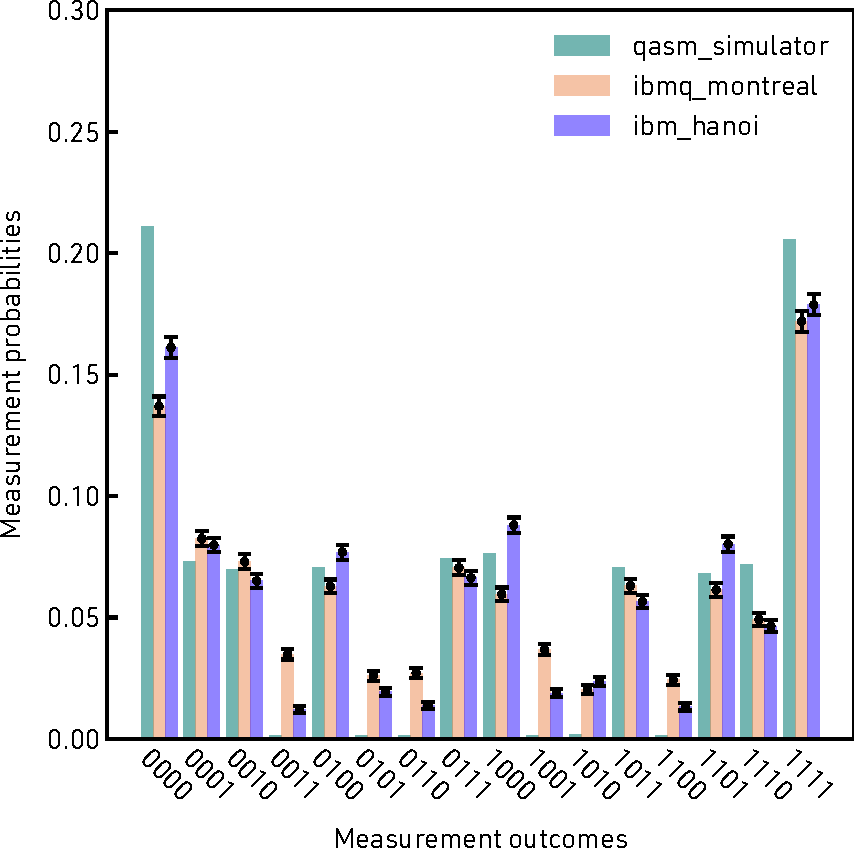
\includegraphics[width=0.86\textwidth]{K14_outcomes}
    \caption[Results of the \acs{max-cut} problem for the star graph $K_{1,4}$ on IBM Q processors.][50pt]{Results of the \acs{max-cut} problem for the star graph $K_{1,4}$ on IBM Q processors. The four-qubit circuit in~\protect\refFigureOnly{grover_k14} is used where the qubit for vertex $0$ is not included as described in the main text. On each processor, the circuit was executed ${8192 \times 900}$ times with measurement error mitigation. The error bars represent ${95\%}$ confidence intervals around the mean value of each histogram bin (See~\protect\refSectionOnly{error_bars} of technical~\protect\refAppendixOnly{appendix_A} for details). The simulator probabilities show the ideal case.}
    \labelFigure{K14_outcomes}
\end{figure}

\clearpage
\noindent
Compared to the results in the study~\cite{Satoh_2020}, they represent an improvement as they exceed $0.11$ for the \acs{max-cut} solution. However, the comparison is a bit unfair, as the improvement of the results is probably indicative of the improvement of the capabilities of the IBM Q processors more than anything else, as the study~\cite{Satoh_2020} used earlier processors that could only tolerate lower two-qubit gates in a circuit than the currently reported $30$ two-qubit gate limit for current IBM Q processors~\cite{Gwinner_2020,Zhang_2021}. More importantly, our transpiled circuit uses $6$ more controlled-NOT gates. 

\bigskip
\noindent
We now improve the maximum ideal probability for measuring the \acs{max-cut} by using a further Grover iterate that uses a local diffuser operator as shown in~\refFigureOnly{grover_k14_mod}. The circuit is mapped to a physical device using the same mapping as in~\refFigureOnly{K14_mappings}~\refSubfigureOnly{K14_mod_mapping} as before, with the controlled-NOT gates in the transpiled circuit tallying to $33$. 

\begin{figure}[h]
	\centering
	\resizebox{1.0\textwidth}{!}{%
	\begin{tikzpicture}
		\begin{yquant}[register/separation=4mm]
			qubit {$q_{\idx}$} q[4];


			[this subcircuit box style={draw, dashed, inner ysep=6pt, label=above:$O(\theta_0)$}]
			subcircuit {
				qubit {} q[4];
				box {$R_z(\theta_0)$} q;
			} (q);


			[this subcircuit box style={draw, dashed, inner ysep=6pt, label=above:$D_{4,3}$}]
			subcircuit {
				qubit {} q[3];
				x q[0-2];
				h q[0-2];
				box {$Z$} q[2] | q[0-1];
				h q[0-2];
				x q[0-2];

			} (q[0-2]);

			[this subcircuit box style={draw, dashed, inner ysep=6pt, label=above:$O(\theta_1)$}]
			subcircuit {
				qubit {} q[4];
				box {$R_z(\theta_1)$} q;
			} (q);


			[this subcircuit box style={draw, dashed, inner ysep=6pt, label=above:$D_4$}]
			subcircuit {
				qubit {} q[4];
				x q;
				h q;
				box {$Z$} q[3] | q[0-2];
				h q;
				x q;
			} (q);
			measure q;
		\end{yquant}
	\end{tikzpicture}
	}
	\caption[A circuit diagram for the \acs{max-cut} problem for the star graph $K_{1,4}$ realized on four qubits that uses two Grover iterates improves over the ideal probability of \acs{max-cut} in the study~\cite{Satoh_2020}.]{A circuit diagram for the \acs{max-cut} problem for the star graph $K_{1,4}$ realized on four qubits that uses two Grover iterates improves over the ideal probability of \acs{max-cut} in the study~\cite{Satoh_2020}. Here, one local Grover iterate $G_{4,3}(\theta_0)$ where ${\theta_0\simeq 0.323\pi}$ and a global Grover iterate $G_{4}(\theta_1)$ where ${\theta_1\simeq 0.322\pi}$ yield an ideal probability of observing the \acs{max-cut} outcome close to $0.25$ upon measuring all the qubits in the computational basis.}
	\labelFigure{grover_k14_mod}
\end{figure}

\noindent
We choose the values $\theta_0=\theta_1 \simeq 0.323 \pi$ (more on this choice later ), for this choice the ideal probability of measuring the \acs{max-cut} is close to $0.25$. ~\refFigureOnly{K14_mod_outcomes} shows the readout error mitigated results of measurement outcomes from the two processors. 

\begin{figure}[h]
    \centering
    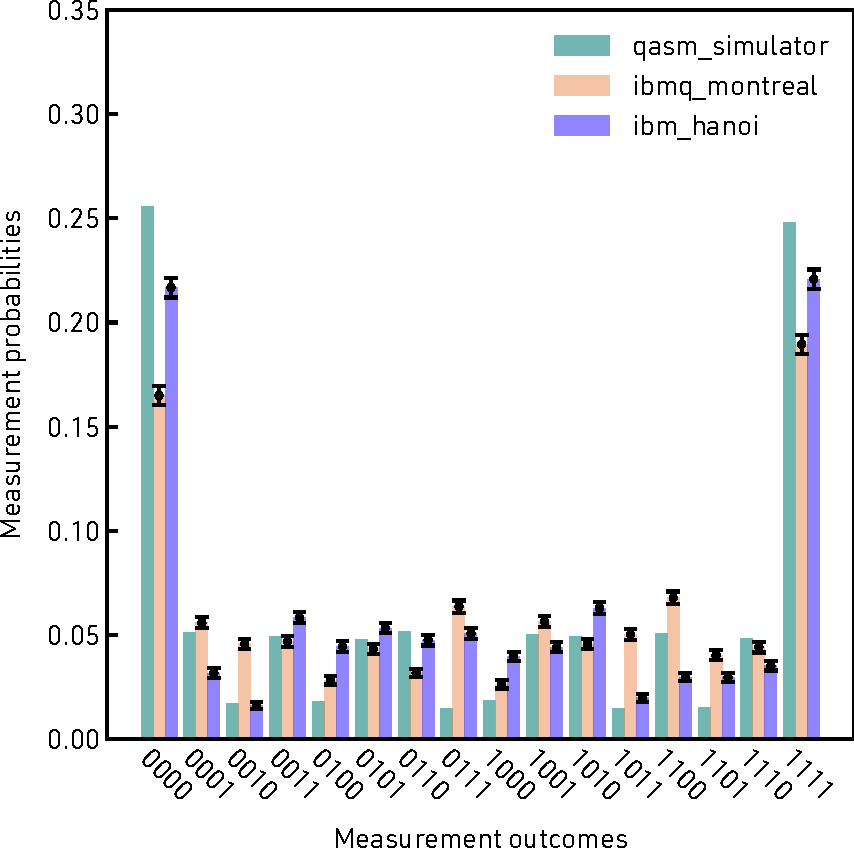
\includegraphics[width=.86\textwidth]{K14_mod_outcomes}
    \caption[Results of the \acs{max-cut} problem with two Grover iterates for the star graph $K_{1,4}$ on IBM Q processors.]{Results of the \acs{max-cut} problem with two Grover iterates for the star graph $K_{1,4}$ on IBM Q processors. The four-qubit circuit in~\protect\refFigureOnly{grover_k14_mod} is used where the qubit for vertex $0$ is not included as described in the main text. On each processor, the circuit was executed ${8192 \times 900}$ times with measurement error mitigation. The error bars represent ${95\%}$ confidence intervals around the mean value of each histogram bin (See~\protect\refSectionOnly{error_bars} of technical~\protect\refAppendixOnly{appendix_A} for details). The simulator probabilities show the ideal case.}
    \labelFigure{K14_mod_outcomes}
\end{figure}

\clearpage
\noindent
The \acs{max-cut} outcome $1111$, and the no-cut outcome $0000$ ($00000$ and $01111$ respectively since virtual vertex $0$ is set to $0$), occur with probability close to $0.16$ and $0.19$, respectively on the \textbf{ibmq\_montreal} processor. And occur with probability close to $0.22$ and $0.22$, respectively on the \textbf{ibm\_hanoi} processor. The Kolmogorov distance between the measured distribution and the ideal distribution is $0.1308$ and $0.1844$ for \textbf{ibmq\_montreal} and \textbf{ibm\_hanoi}, respectively. With an additional local diffuser operator, we have slightly improved over the results in~\refFigureOnly{K14_outcomes}. At the time of writing this thesis, it dawned on the author that the choice of angles $\theta_0$ and $\theta_1$ as $0.323\pi$ for the circuit~\refFigureOnly{grover_k14_mod} do not necessarily achieve the maximum possible ideal probability of measuring the \acs{max-cut} any more. The choice $\theta_0 \simeq 0.301 \pi$ and $\theta_1 \simeq 0.541 \pi$ for the circuit shown in~\refFigureOnly{grover_k14_mod} yields a maximum ideal probability for measuring the \acs{max-cut} close to $0.311$. Interestingly, another revelation that occurred to the author is that the local diffuser operator $D_{4,3}$ in~\refFigureOnly{grover_k14_mod} can be replaced with a smaller local diffuser operator $D_{4,2}$ as shown in~\refFigureOnly{grover_k14_modd}. Choosing the angles $\theta_0$ and $\theta_1$ as $0.359\pi$ and $0.814\pi$, respectively yields a probability of measuring the \acs{max-cut} close to $0.2482$.

\begin{figure}[h]
	\centering
	\resizebox{1.0\textwidth}{!}{%
	\begin{tikzpicture}
		\begin{yquant}[register/separation=4mm]
			qubit {$q_{\idx}$} q[4];


			[this subcircuit box style={draw, dashed, inner ysep=6pt, label=above:$O(\theta_0)$}]
			subcircuit {
				qubit {} q[4];
				box {$R_z(\theta_0)$} q;
			} (q);


			[this subcircuit box style={draw, dashed, inner ysep=6pt, label=above:$D_{4,2}$}]
			subcircuit {
				qubit {} q[2];
				x q[0-1];
				h q[0-1];
				box {$Z$} q[1] | q[0];
				h q[0-1];
				x q[0-1];

			} (q[0-1]);

			[this subcircuit box style={draw, dashed, inner ysep=6pt, label=above:$O(\theta_0)$}]
			subcircuit {
				qubit {} q[4];
				box {$R_z(\theta_1)$} q;
			} (q);


			[this subcircuit box style={draw, dashed, inner ysep=6pt, label=above:$D_4$}]
			subcircuit {
				qubit {} q[4];
				x q;
				h q;
				box {$Z$} q[3] | q[0-2];
				h q;
				x q;
			} (q);
			measure q;
		\end{yquant}
	\end{tikzpicture}
	}
	\caption[A circuit diagram for the \acs{max-cut} problem for the star graph $K_{1,4}$ realized on four qubits that uses two Grover iterates improves over the ideal probability of \acs{max-cut} in the study~\cite{Satoh_2020} even with a smaller local diffuser operator compared to ~\protect\refFigureOnly{grover_k14}.]{A circuit diagram for the \acs{max-cut} problem for the star graph $K_{1,4}$ realized on four qubits that uses two Grover iterates improves over the ideal probability of \acs{max-cut} in the study~\cite{Satoh_2020} even with a smaller local diffuser operator compared to ~\protect\refFigureOnly{grover_k14}. Here one local Grover iterate $G_{4,2}(\theta_0)$ where ${\theta_0 \simeq 0.359\pi}$ and global Grover iterate $G_{4}(\theta_1)$ where ${\theta_1 \simeq 0.814\pi}$ yields an ideal probability of observing the \acs{max-cut} outcome close to $0.2482$ upon measuring all the qubits in the computational basis.}
	\labelFigure{grover_k14_modd}
\end{figure}

\noindent
Unfortunately, the author realized the aforementioned possibilities quite late in their thesis writing when they returned to the \acs{max-cut} problem and could not test the two circuits in shown~\refFigureOnly{grover_k14_mod} and~\refFigureOnly{grover_k14_modd} on the IBM Q processors in time. However, it is not too far-fetched to think that the results would slightly improve over the ones presented here, even more so, for the circuit in~\refFigureOnly{grover_k14_mod}, since it would be transpiled to a circuit with fewer two-qubit gates. This combination of local and global diffuser operators together with a subdivided oracle $O(\theta)$, where the $\theta$ are optimized at each stage to maximize the probability of observing the \acs{max-cut} solution, is an interesting direction for future work in realizing the \acs{max-cut} problem on \acs{NISQ} processors. 


\bigskip
\noindent
However, it is unlikely that such an algorithm can be still considered as Grover's algorithm because we modify the angles of the oracle at each step by classically finding the optimal angles $\theta_i$ for the oracle $O(\theta_i)$ that achieve maximum probability of observing the desired outcome at that step. Such an algorithm is comparable to hybrid quantum/classical algorithms such as the \gls{VQE}~\cite{Peruzzo_2014} and \gls{QAOA}~\cite{Farhi_2014}. In a similar fashion, the aforesaid algorithms seek to prepare some desired $n$-qubit state $\ket{\psi}$ that maximizes/minimizes some objective cost function. In the case of \acs{VQE}, the desired state $\ket{\psi}$ is one that minimizes the expectation value $\expval{H}{\psi}/\ip{\psi}$ with respect to some Hamiltonian $H$. For \acs{QAOA},  $\ket{\psi}$ maximizes some cost function for an optimization problem such as the \acs{max-cut} (see Ref.~\cite{Farhi_2014} details). 

\bigskip
\noindent
For both algorithms at each step, a sequence of gates $U_1(\theta_1)U_2(\theta_2)\cdots U(\theta_n)$ parameterized with tunable parameter(s) $\vec{\theta}$ is applied to the current best approximation of $\ket{\psi}$ after which, a quantum computer evaluates the objective function and the classical computer aids by optimizing the parameters $\vec{\theta}$ for the next evaluation step. For the previously described scheme, the oracle $O(\theta)$ can be viewed as the $U_1(\theta)U_2(\theta)\cdots U(\theta)$ and the objective cost function is $p(\theta)$ from~\refEquationOnly{p_theta}. Recently, such a hybrid quantum/classical approach to Grover's canonical search algorithm has been considered in the study~\cite{Morales_2018}. For a parametrized phase oracle and non-parametrized diffuser (and other), such a hybrid approach achieves a better success probability than Grover's algorithm canonical quantum search for small search space size $N$, asymptotically both algorithms have the same performance~\cite{Morales_2018}.

\subsection{Quantum search in measurement-based quantum computing}
\labelSection{C2_quantum_search_in_measurement_based_quantum_computing}

The experimental demonstrations of Grover's algorithm have also been realized in the context of \gls{MBQC} on graph states. The canonical quantum search algorithm on two qubits has been experimentally realized by different studies thus far~\cite{Walther_2005,Prevedel_2007,Chen_2007,Barz_2012} on a four-qubit graph state. Common among the aforementioned references, is the realization that the canonical quantum search algorithm on two qubits naturally arises as a measurement procedure on a four-qubit box graph state shown in~\refFigureOnly{box_graph}.

\begin{marginfigure}
	\centering
	\tikzfig{graphics/box_graph}
    \caption[Four qubit box graph state realized by first preparing all qubits in the $\ket{+}$, and then applying controlled-$Z$ gates between qubits with edges connecting them.]{Four qubit box graph state realized by first preparing all qubits in the $\ket{+}$, and then applying controlled-$Z$ gates between qubits with edges connecting them.}
	\labelFigure{box_graph}
\end{marginfigure}

\bigskip
\noindent
Recall that in~\acs{MBQC}, gates are simulated by performing measurements on an initially prepared graph state in the equatorial measurement basis $B(\alpha) = \{ \ket{+\alpha},\ket{-\alpha}\}$, where $\ket{\pm \alpha}_j = (\ket{0}_j \pm e^{i\alpha}\ket{1})$. Thus if we measure qubits $0$ and $3$ in the basis $B_0(\alpha)$ and $B_3(\beta)$, respectively. This set of measurements effectively applies the $(X^{m_0} H R_z(\alpha))^{(q_0)} \otimes(X^{m_3} H R_z(\beta))^{(q_3)}CZ_{q_{0}q_{3}}$ on qubits $\ket{q_0}$ and qubit $\ket{q_3}$ of graph state shown in~\refFigureOnly{box_graph}~\footnote{See Ref.\cite{Jozsa_2005,Nielsen_2006,Browne_2016} for detailed descriptions of \acs{MBQC}.}. The values $m_0, m_3 \in \{0,1\}$ denote measurement outcomes of the preceding measurements outcomes where a value of $m_i=0$ or $m_i=1$ indicates that we measured the $\ket{+\alpha}$ or $\ket{-\alpha}$ state, respectively, on qubit $i$. Lastly, we perform the measurement $B(\pi)$ on both qubits $1$ and $2$. 

%p \begin{figure}[h]
% 	\centering
% 	\resizebox{1.0\textwidth}{!}{%
% 	\begin{tikzpicture}
% 		\begin{yquant}[register/separation=4mm]
% 			qubit {$\ket{q_0}=\ket{+}$} q0;
% 			qubit {$\ket{q_1}=\ket{+}$} q1;
% 			qubit {$\ket{q_2}=\ket{+}$} q2;
% 			qubit {$\ket{q_3}=\ket{+}$} q3;

% 			box {$Z$} q1 | q0;
% 			box {$Z$} q2 | q1;
% 			box {$Z$} q3 | q2;
% 			box {$Z$} q3 | q0;


% 			[this subcircuit box style={draw, dashed, inner ysep=6pt, label=above:$B_0(\alpha)$}]
% 			subcircuit {
% 				qubit {} q0;
% 				box {$R_z(\alpha)$} q0;
% 				h q0;
% 				measure q0;
% 			} (q0);

% 			[this subcircuit box style={draw, dashed, inner ysep=6pt, label=below:$B_3(\beta)$}]
% 			subcircuit {
% 				qubit {} q3;
% 				box {$R_z(\beta$)} q3;
% 				h q3;
% 				measure q3;
% 			} (q3);

% 			box {$R_z(\alpha) H X^{m_0}$} q1 | q0;
% 			box {$R_z(\beta) H X^{m_2}$}  q2 | q3;

% 			discard q1;
% 			discard q2;

% 			init {$X^{m_0} H R_z(\alpha) \ket{q_0}$} q1;
% 			init {$X^{m_3}  H R_z(\beta) \ket{q_3}$} q2;

% 			box {$R_z(\pi)$} q1;
% 			h q1;

% 			box {$R_z(\pi)$} q2;
% 			h q2;

% 			measure q1;
% 			measure q2;
% 		\end{yquant}
% 	\end{tikzpicture}
% 	}
% 	\caption[A circuit diagram equivalent of the measurement procedure on a four qubit graph state realizes Grover's two-qubit quantum search algorithm.]{A circuit diagram equivalent of the measurement procedure on a four qubit graph state realizes Grover's two-qubit quantum search algorithm; the circuit begins by measuring qubits $0$ and $3$ in the basis $B(\alpha)$ and $B(\beta)$ respectively, which effectively applies $X^{m_a} H R_z(\theta)$ to each qubit, where $m_a$ is the measurement outcome on qubit $a$. After which, the resultant joint state on qubit $0$ and $3$ is teleported to qubit $1$ and $2$, respectively. The final round of measurements is on qubits $1$ and $2$, which we both measure in the basis $B(\pi)$.}
% 	\labelFigure{4q_graph_state_circ}
% \end{figure}

\bigskip
\noindent
It is useful to write $X^{m_a} H R_z(\theta)$ as $H Z^{m_a} R_z(\theta)$ where we use the identity $X H = H Z$. From this, the effective two-qubit state after the above measurement procedure that resides on qubits $2$ and $3$ is equivalent to the circuit diagram shown in~\refFigureOnly{2q_grover} in the quantum circuit model. The aforementioned circuit realizes Grover quantum search algorithm on two qubits for an appropriate choice of the angles $\alpha$ and $\beta$, in the case where $m_0=m_3=0$. For the choice of angles $(\alpha, \beta) = (-\pi,-\pi), (-\pi, 0), (0,-\pi)$ and $(0,0)$, the phase oracle puts a negative sign on the amplitude of the state $\ket{00}, \ket{01}, \ket{10}$ and $\ket{11}$, respectively. For any combination of $m_0,m_3$, the above circuit still realizes Grover's algorithm with an appropriate reinterpretation of the measurement outcomes. The interested reader may refer to section~\refSectionOnly{grover_equivalence_mbqc} of the technical~\refAppendixOnly{appendix_B} for more details.

\begin{figure}[h]
	\centering
	\begin{tikzpicture}
		\begin{yquant}[register/separation=4mm]
			qubit {$\ket{q_0}=\ket{+}$} q0;
			qubit {$\ket{q_1}=\ket{+}$} q1;

			[this subcircuit box style={draw, dashed, inner ysep=6pt, label=above:Phase oracle}]
			subcircuit {
 				qubit {} q0;
 				qubit {} q1;

 				box {$Z$} q1 | q0;
 				box {$R_z(\alpha)$} q0;
 				box {$R_z(\beta)$} q1;
				box {$Z^{m_0}$} q0;
				box {$Z^{m_3}$} q1;
			} (q0, q1);

			[this subcircuit box style={draw, dashed, inner ysep=6pt, label=above:Diffuser}]
			subcircuit {
				qubit {} q0;
				qubit {} q1;

				h q0, q1;
				box {$Z$} q1 | q0;
				z q0;
				z q1;
				h q0, q1;
			} (q0, q1);

			measure q0, q1;
		\end{yquant}
	\end{tikzpicture}
	\caption[A circuit diagram equivalent of the remaining two qubit after the four-qubit measurement procedure descibed in the main text.]{A circuit diagram equivalent of the remaining two qubit after the four-qubit measurement procedure described in the main text; the resultant circuit realizes Grover's algorithm for two qubits with the appropriate choice of angles $\alpha$ and $\beta$. For ${(\alpha, \beta) = (-\pi,-\pi), (-\pi, 0), (0,-\pi)}$ and $(0,0)$ the circuit finds the target $\ket{00}, \ket{01}, \ket{10}$ and $\ket{11}$ respectively.}
	\labelFigure{2q_grover}
\end{figure}

\clearpage
\noindent
In my honours studies, we realized the above measurement-based Grover's algorithm for two qubits successfully on IBM Q processors. Additionally, we were able to realize a measurement-based Grover's algorithm for two qubits on a graph state with one fewer edge, thus one less two-qubit gate in its state preparation. The original four-qubit graph state and the latter graph state belong to the same \acs{LU}-equivalence class~\cite{Hein_2004, Nest_2004}. The local unitaries relating the two states can be derived by successive applications of the edge local complementation rule~\cite{Hein_2004,Nest_2004}. For the interested reader, the missing details are filled in sections~\refSectionOnly{grover_equivalence_mbqc} and ~\refSectionOnly{4q_lu_equiv_meas_proc} of the technical~\refAppendixOnly{appendix_B}.

\bigskip
\noindent
Hence, we considered the next natural step; whether it would be possible to realize a measurement-based Grover's algorithm for three qubits. The initial hurdle was that the quantum circuit model equivalent of Grover's algorithm on three qubits does not naturally arise as a measurement procedure on any well known graph state unlike the case for two qubits, as far as we are aware. An unsophisticated way to circumvent this hurdle is to look for measurement-based implementations of the various gates in the quantum circuit model of Grover's algorithm for three qubits, and thus by constructing the measurement-based equivalent of each gate in the circuit and linking them together, one can realize the entire circuit as a measurement-based procedure.

\begin{marginfigure}
	\centering
    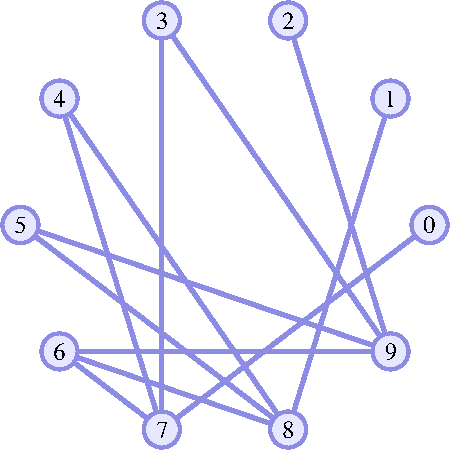
\includegraphics[width=0.65\textwidth]{10q_graph_state}
    \caption[Ten-qubit graph state used as a resource for realizing a measurement-based controlled-controlled-$Z$ gate.]{Ten-qubit graph state used as a resource for realizing a measurement-based three-qubit Toffoli gate. Qubits $0,1,2,6$ are measured in the $H B(\pi/4)$ basis and qubits $3,4,5$ in the $H B(\pi/4)$ basis, which realizes a controlled-controlled-$Z$ gate up to measurement outcome byproducts acting on the inputs in qubits $7,8$ and $9$ as two control and target qubits, respectively.}
	\labelFigure{10q_graph_state}
\end{marginfigure}

\noindent
As we have seen earlier, the $n$-qubit $C^{n-1}[Z]$, in this case, a controlled-controlled-$Z$ gate constitutes the most resourceful part in Grover's algorithm, appearing in both the phase oracle and diffuser operators. The canonical measurement-based controlled-controlled-$Z$ due to Browne and Briegel~\cite{Browne_2016} can be realized on a graph state of ten qubits. The measurement-based controlled-controlled-$Z$ gate is a special case of a general result from the aforementioned reference, any $n$-qubit unitary operator diagonal in the computational basis of the form~\cite{Browne_2016}


\begin{align}
	U_n &= \displaystyle\prod_{\vec{m}} \exp(i \frac{\theta_{\vec{m}}}{2} (Z_1)^{m_1} \otimes (Z_2)^{m_2} \otimes \cdots \otimes (Z_n)^{m_n} ), \nonumber \\
	&= \exp(\frac{i}{2}\displaystyle\sum_{\vec{m}} \theta_{\vec{m}} (Z_1)^{m_1} \otimes (Z_2)^{m_2} \otimes \cdots \otimes (Z_n)^{m_n}),
\end{align}

\noindent
where $m_j \in \{0, 1\}$ and $Z_j$ is the Pauli $Z$ operator acting on qubit $j$. The sum is performed over all possible bit strings of length $n$. From the above form, the controlled-controlled-$Z$ gate is realized by the following choice of angles

\begin{align}
	\theta_{000} = 0, \theta_{001} = -\frac{\pi}{4}, \theta_{010} = -\frac{\pi}{4}, \theta_{011} = \frac{\pi}{4}, \nonumber \\
	\theta_{100} = -\frac{\pi}{4}, \theta_{101} = \frac{\pi}{4}, \theta_{110} = \frac{\pi}{4}, \theta_{111} = -\frac{\pi}{4}.
\end{align}

\noindent
The ten-qubit graph state that realizes the three-qubit Toffoli gate is shown in~\refFigureOnly{10q_graph_state}. The input qubits $7,8$ and $9$ can be prepared in any single-qubit state rather than strictly $\ket{+}$ since qubits $7,8$ and $9$ are designated as input controls and target qubits, respectively, for the \acs{MBQC} controlled-controlled-$Z$ gate. Thus, the procedure to realize a controlled-controlled-$Z$ gate with input qubits $\ket{c_1}, \ket{c_2}, \ket{t}$ as follows: (i) Prepare inputs $\ket{c_1}, \ket{c_2}, \ket{t}$ to any state of our choosing, the rest of the qubits are prepared in the $\ket{+}$, and we perform controlled-$Z$ gates on qubits connected by an edge in~\refFigureOnly{10q_graph_state}. (ii) perform the projective measurements of the $H B(\theta) = \cos{\theta/2}\ket{0}\pm \sin{\theta/2}\ket{1}$, with $\theta=\pi/4$ for qubits $0, 1, 2, 6$ and $\theta=-\pi/4$ for qubits $3,4,5$, respectively~\cite{Browne_2016}. 

\noindent
The above measurement procedure realizes a three qubit controlled-controlled-$Z$ gates acting on the inputs $c_1, c_2, t$ and output of the gate residing on qubits $7,8$ and $9$, up to the byproduct Pauli operators that arise from the measurement outcomes.

\begin{align}
	(Z^{m_0+ m_3 + m_4+m_6})^{(7)} \otimes (Z^{m_1+ m_4+m_5+m_6})^{(8)} \otimes (Z^{m_2}Z^{m_3}Z^{m_5}Z^{m_6})^{(8)},
\end{align}

\noindent
where $m_i \in \{0, 1\}$ is an outcome from the aforementioned measurement procedure on qubit $i$, and the byproducts act on qubits $7,8$ and $9$, respectively.

\begin{marginfigure}
	\centering
	\tikzfig{graphics/10q_mapping}
    \caption[Physical device ten-qubit mapping for the ten-qubit graph state in~\protect\refFigureOnly{10q_graph_state}.]{Physical device ten-qubit mapping for the ten-qubit graph state in~\protect\refFigureOnly{10q_graph_state}; each labeled node in the aforesaid is mapped to the corresponding labeled qubit in this figure.}
	\labelFigure{10q_mapping}
\end{marginfigure}

\bigskip
\noindent
In implementing the described measurement-based controlled-controlled-$Z$ gate on IBM Q, we begin by mapping the graph state to the qubits of a physical device. The graph state in~\refFigureOnly{10q_graph_state} is highly connected, and no physical device exists with such a topology. Thus, we choose to map qubits that have the most connections to the physical qubits that have most connections on the physical device; in~\refFigureOnly{10q_graph_state} the qubits $7,8$ and $9$ have the most edges. We show a physical device mapping in~\refFigureOnly{10q_mapping}, which results in $60$ controlled-NOT gates for the transpiled circuit. Such a number of two-qubits gates in circuit is well-beyond the $30$ two-qubit gate count limit~\cite{Gwinner_2020}, nonetheless we tested the measurement-based controlled-controlled-$Z$ gate by preparing the qubits $7,8$ and $9$ in various input states, and subsequently performed quantum state tomography to recover the corresponding output states, and then measured the state fidelity of each of the recovered output states against a set of expected output states. From these measurements, we are able to construct a truth table for the controlled-controlled-$Z$ gate for various input and output states, this is shown in~\refFigureOnly{MBQC_toff}. As seen can be seen by the naked eye, the discrepancies between the ideal truth tables and measured truth tables on the \textbf{ibmq\_montreal} and \textbf{ibmq\_mumbai} are quite conspicuous.  We show the greatest element difference between the ideal and the measured truth tables for both processors in~\refTableOnly{element_diff}. The fourth truth table shows the smallest value among the truth tables, which corroborates with the visual representation of the fourth truth table in~\refFigureOnly{MBQC_toff}, as it bears somewhat of an resemblance to the corresponding ideal truth table. 

\begin{table}[h!]
	\centering
	\labelTable{element_diff}
	\caption[The maximum element difference between a measure truth table and corresponding ideal truth table for the truth tables of measurement-based controlled-controlled-$Z$ in~\protect\refFigureOnly{MBQC_toff}.]{The maximum element difference between a measured truth table and corresponding ideal truth table for the truth tables of measurement-based controlled-controlled-$Z$ in~\protect\refFigureOnly{MBQC_toff}. }
	\begin{tabular}{ccc}
		\toprule
		 Figures & $\mathcal{E}_\text{mumbai} - \mathcal{E}_\text{ideal}$ & $\mathcal{E}_\text{montreal} - \mathcal{E}_\text{ideal}$ \\
		\toprule
		(b) and (c)  & $0.427$      &  $0.395$ \\
		(e) and (f)  & $0.401$      &  $0.336$ \\ 
		(h) and (i)  & $0.435$      &  $0.353$ \\
		(k) and (l)  & $0.308$      &  $0.268$ \\
		\toprule
	\end{tabular}
\end{table}

\bigskip
\noindent
Similar to the case for the four-qubit graph realizing Grover's algorithm for two qubits, we can hope to reduce the number of controlled-$Z$ operations we have to apply to create the ten-qubit graph state shown in~\refFigureOnly{10q_graph_state} by finding an \acs{LU}-equivalent graph state with fewer edges. However, it turns out that the graph state in~\refFigureOnly{10q_graph_state} corresponds to the one with the least number of edges in its \acs{LU}-equivalence class.  See the technical appendix~\refAppendixOnly{appendix_B} for details. Thus at the present moment a measurement-based implementation of a controlled-controlled-$Z$ is beyond the reach of current \acs{NISQ} processors. Which subsequently also puts realization of a measurement-based Grover's algorithm for three qubits beyond reach, since at least two controlled-controlled-$Z$ and a few single qubit gates are required to realize Grover's quantum search algorithm for three qubits.

\clearpage

\begin{figure*}[t!]
    \centering
	\subfloat[]
	{
		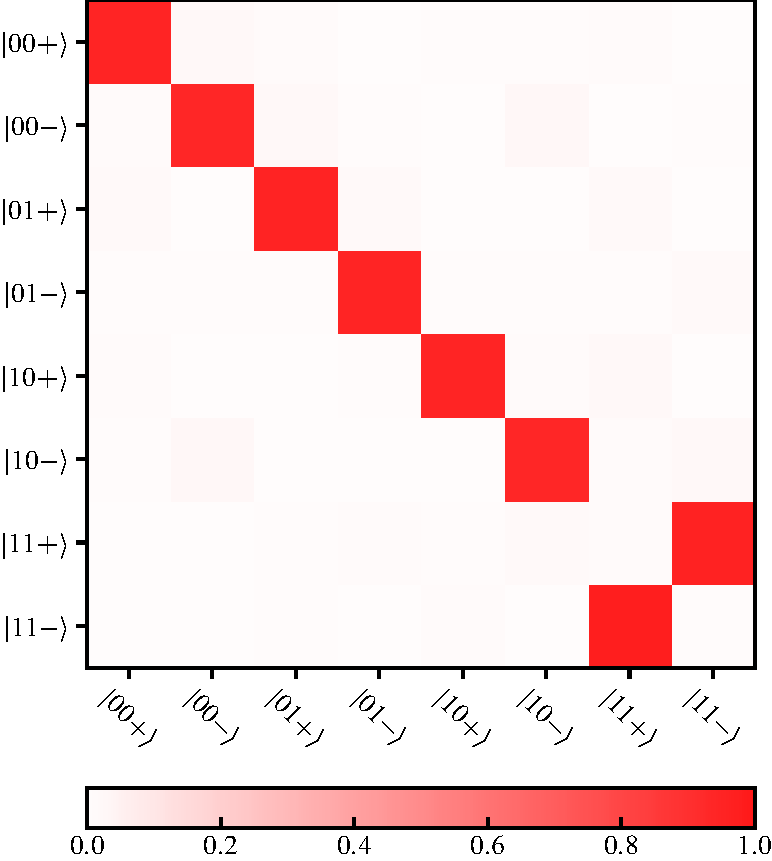
\includegraphics[width=0.33\linewidth]{MBQC_toff_ideal_k0}
	} 
	\subfloat[]
	{
		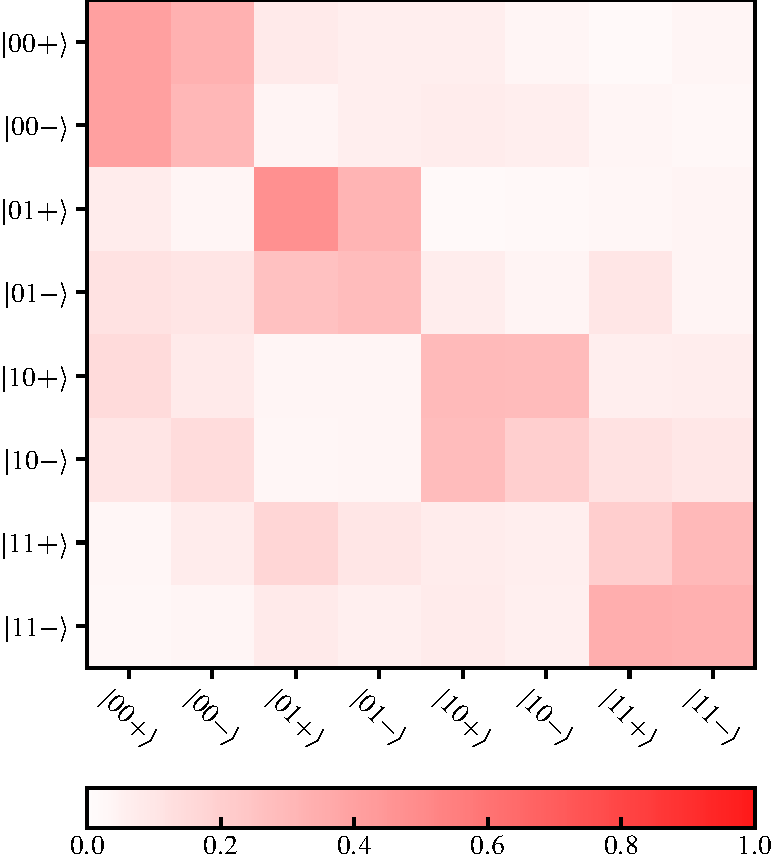
\includegraphics[width=0.33\linewidth]{MBQC_toff_montreal_k0}
	}
	\subfloat[]
	{
		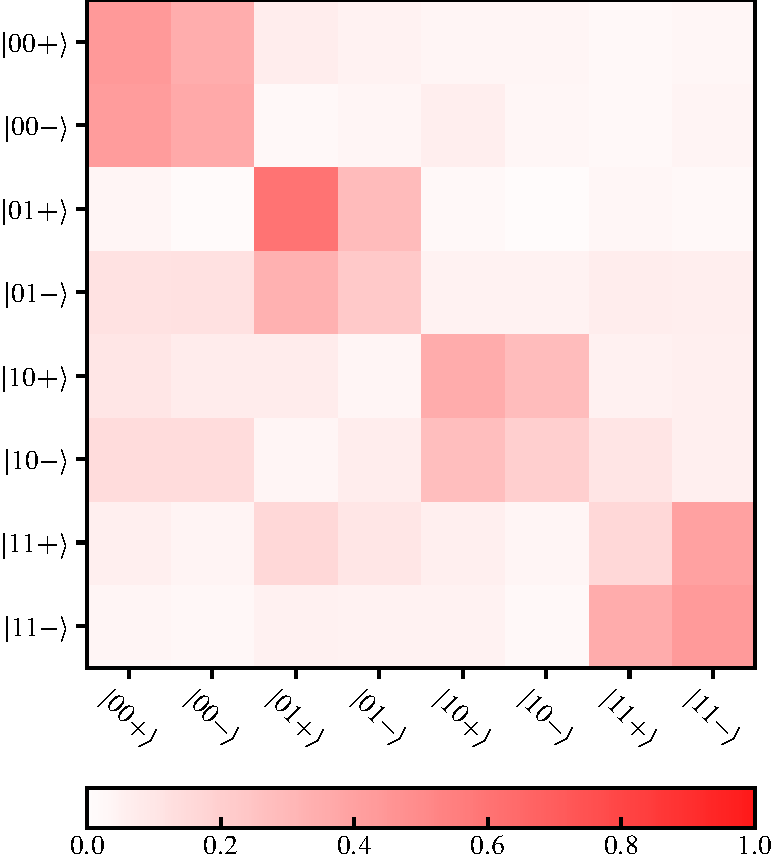
\includegraphics[width=0.33\linewidth]{MBQC_toff_mumbai_k0}
	} \\
	\subfloat[]
	{
		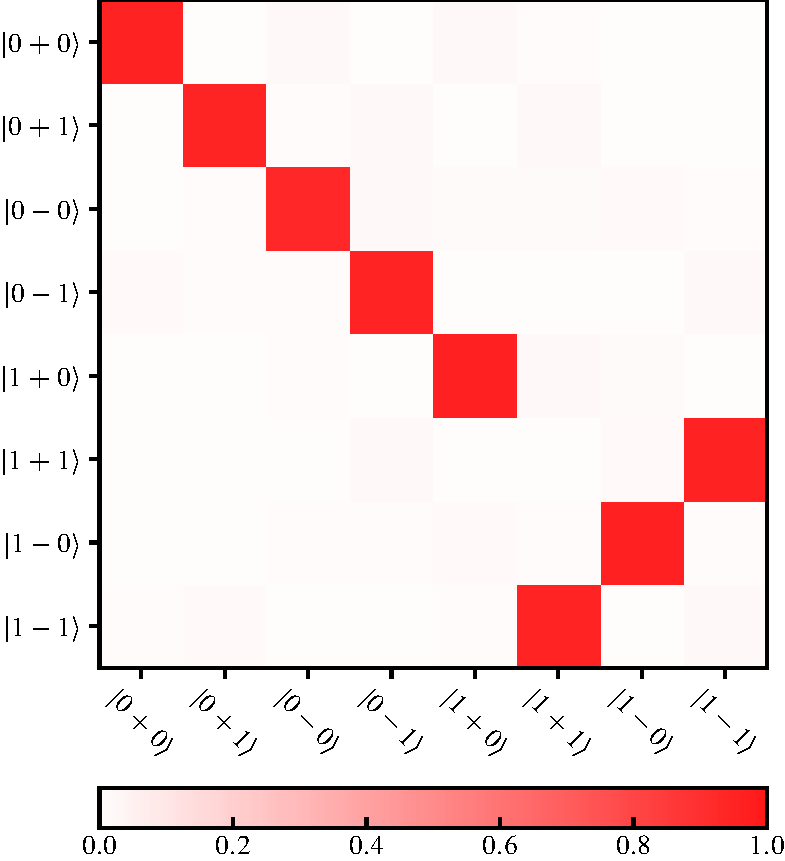
\includegraphics[width=0.33\linewidth]{MBQC_toff_ideal_k1}
	} 
	\subfloat[]
	{
		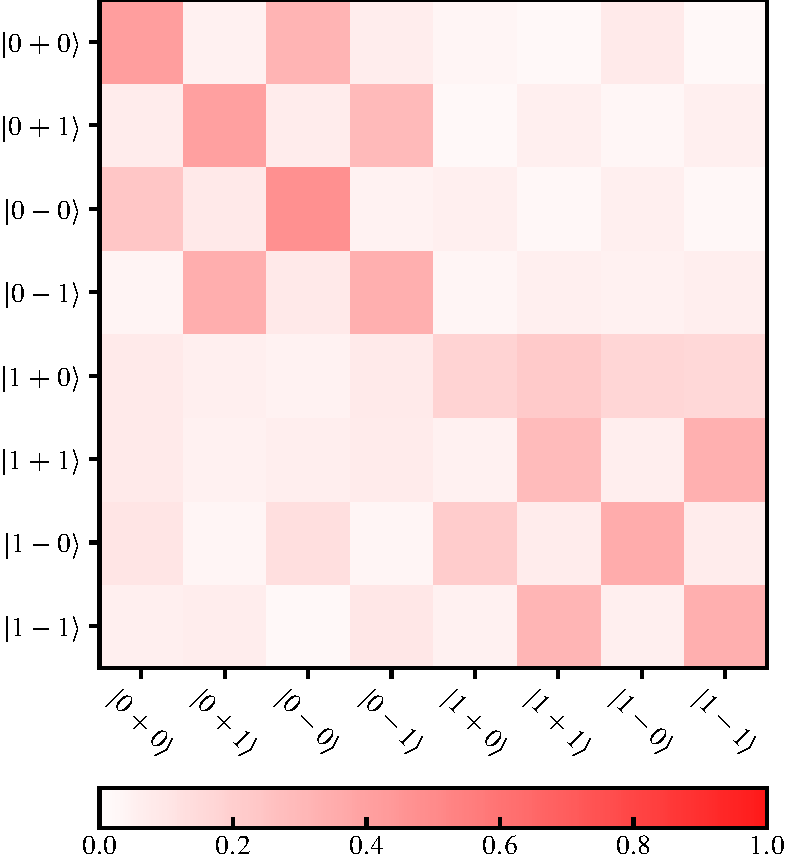
\includegraphics[width=0.33\linewidth]{MBQC_toff_montreal_k1}
	}
	\subfloat[]
	{
		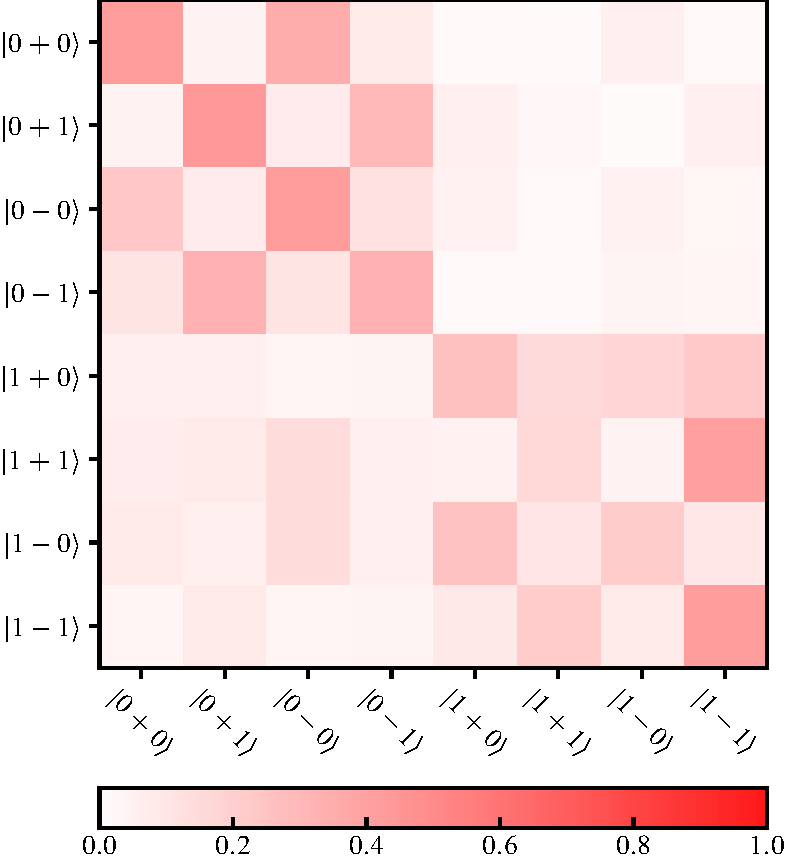
\includegraphics[width=0.33\linewidth]{MBQC_toff_mumbai_k1}
	}  \\
	\subfloat[]
	{
		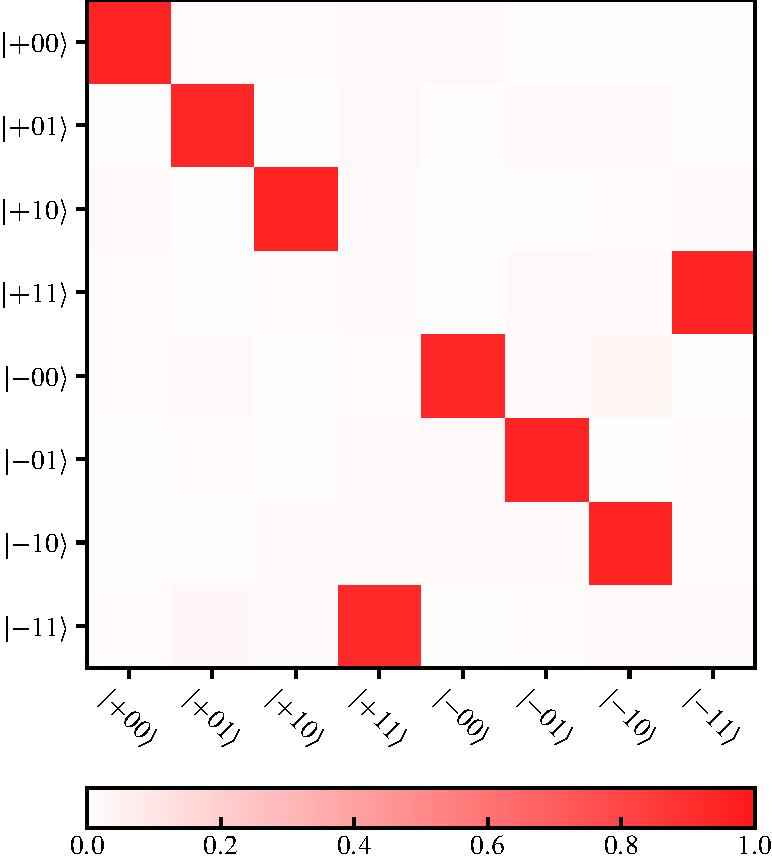
\includegraphics[width=0.33\linewidth]{MBQC_toff_ideal_k2}
	} 
	\subfloat[]
	{
		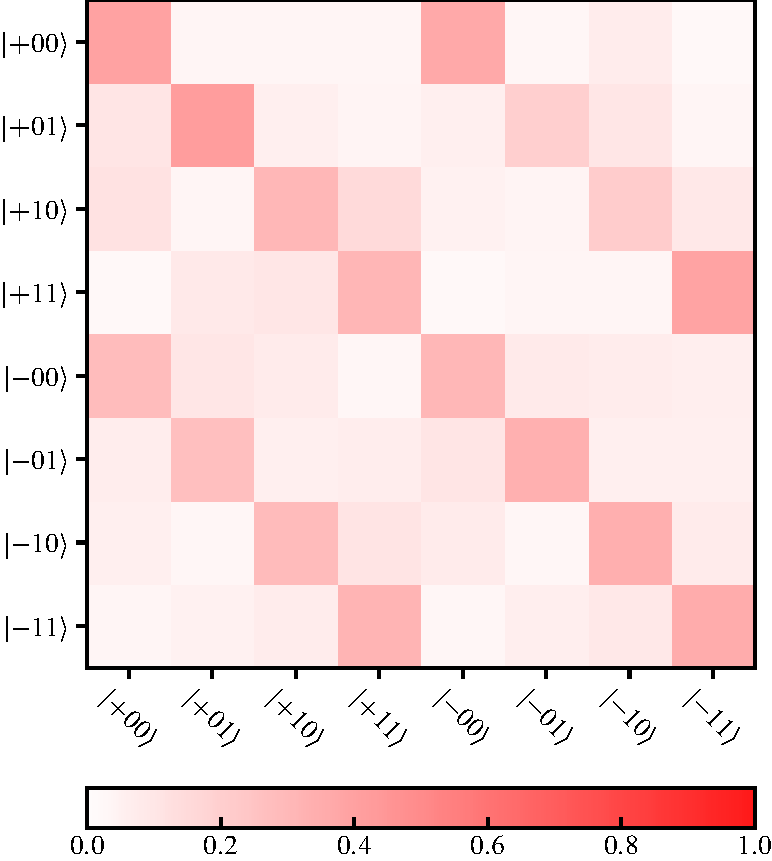
\includegraphics[width=0.33\linewidth]{MBQC_toff_montreal_k2}
	}
	\subfloat[]
	{
		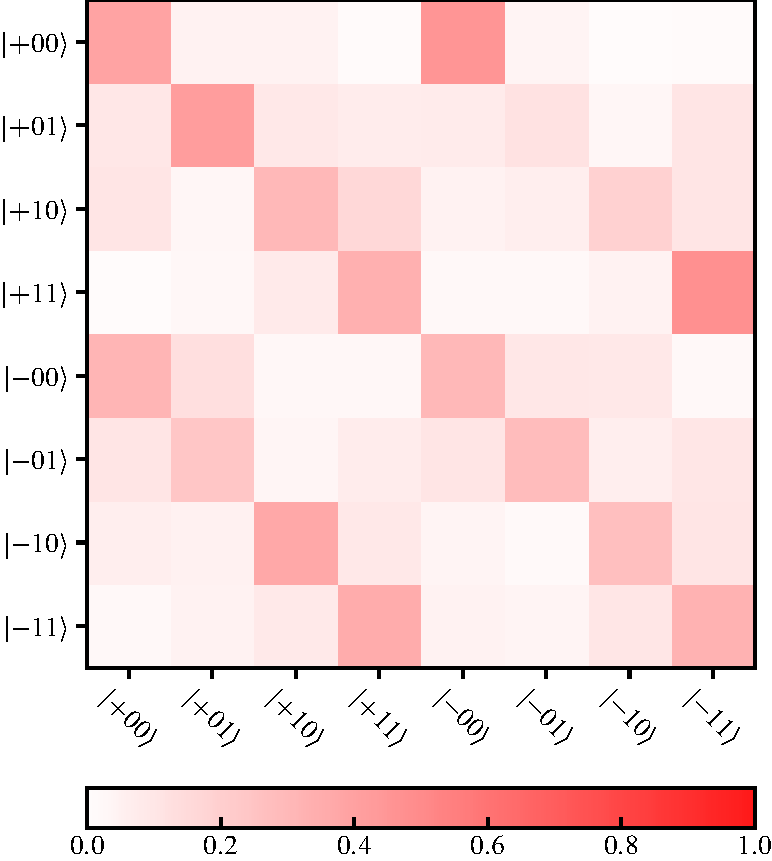
\includegraphics[width=0.33\linewidth]{MBQC_toff_mumbai_k2}
	}
\end{figure*}
\mbox{}
\vfill
\begin{figure*}[t!]
	\setcounter{subfigure}{9}
	\subfloat[]
	{
		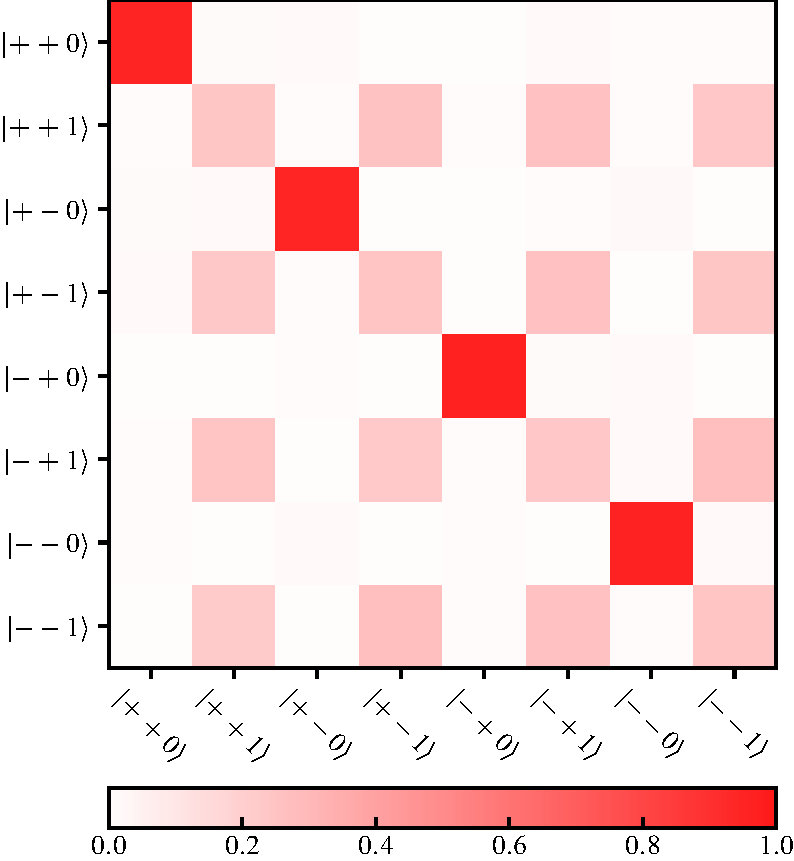
\includegraphics[width=0.33\linewidth]{MBQC_toff_ideal_k3}
	} 
	\subfloat[]
	{
		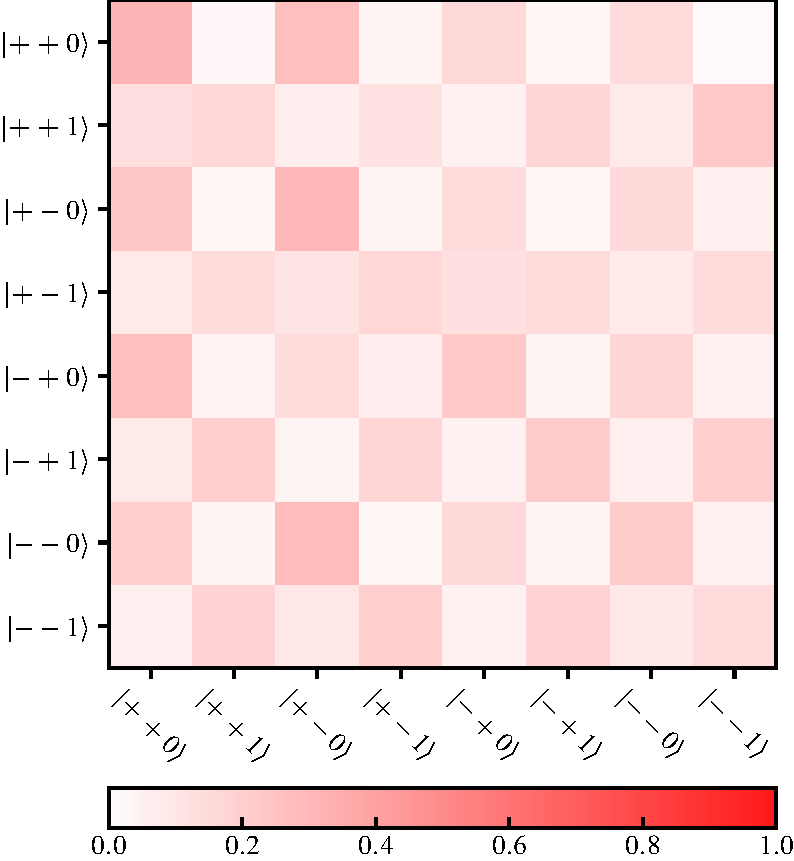
\includegraphics[width=0.33\linewidth]{MBQC_toff_montreal_k3}
	}
	\subfloat[]
	{
		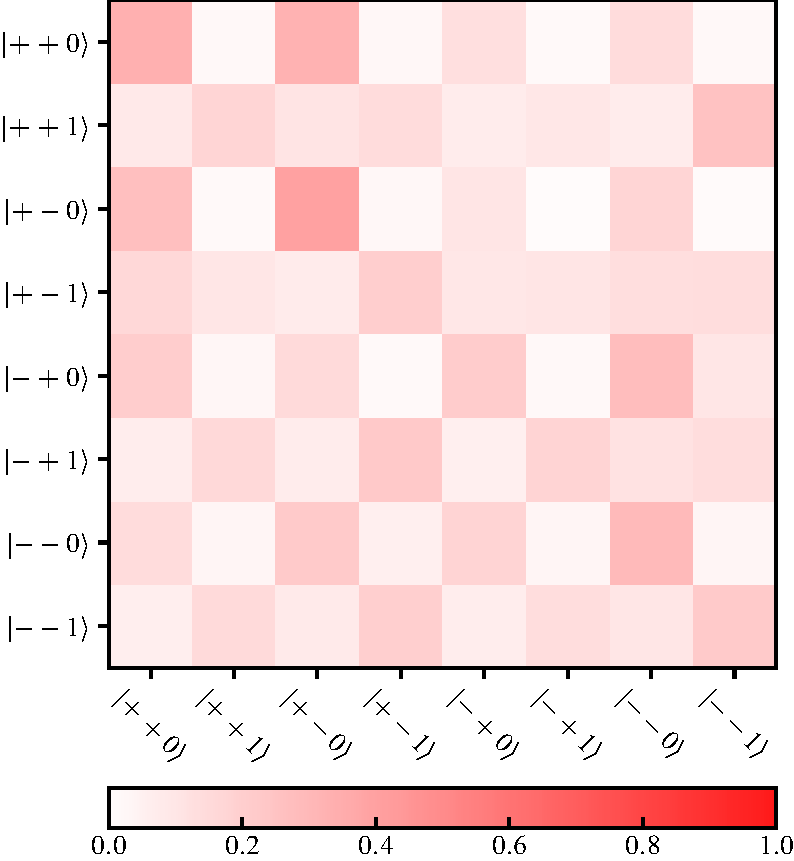
\includegraphics[width=0.33\linewidth]{MBQC_toff_mumbai_k3}
	}
	\caption[Various truth tables for the measurement-based three-qubit controlled-controlled-$Z$ gate.]{Various truth tables for the measurement-based three-qubit controlled-controlled-$Z$ gate. Three figures in each row show a single truth table showing the ideal truth table and measured truth tables from the \textbf{ibmq\_montreal} processor and the measured truth tables from \textbf{ibmq\_mumbai} processor, respectively. When performing the state tomography on the outputs of the gate, we only consider where all the outcomes on the measured qubits are $0$, resulting in no byproducts. \textbf{(a, d, g, j)} Ideal truth tables. \textbf{(b,e,h,k)} Measured truth tables from the processor \textbf{ibmq\_montreal}. \textbf{(c, f, i, l)} Measured truth tables from the processor \textbf{ibmq\_mumbai}.}
	\labelFigure{MBQC_toff}
\end{figure*}


\section{Concluding remarks}
\labelSection{C2_concluding_remarks}

\noindent
 In this chapter, we first began by describing the canonical quantum search algorithm, which assumes no \emph{a priori} knowledge about the structure of the search problem. Such a quantum search algorithm achieves a quadratic speedup over an exhaustive classical search~\cite{Grover_1997}. We also described a variant of the quantum search algorithm called the partial search quantum algorithm, which trades accuracy for speed by finding a partial bit string or target block to which the target element belongs rather than the target element itself~\cite{Grover_2005}. With regards to practicality, especially on \acs{NISQ} processors, the appealing feature of the quantum partial search algorithms in comparison to the canonical quantum search is that they are economical in the number of elementary gates and algorithmic steps they use, albeit the above advantage comes at the expense of accuracy. This realization prompted a large corpus of work interested in realizing small-scale demonstrations of the quantum search algorithm for four qubits and beyond, by reducing the number of elementary operations, particularly two-qubit gates, in quantum search algorithms.

 \bigskip
 \noindent
 Two important theoretical results along these lines were the depth-optimization of the quantum search algorithm, and multi-stage quantum search~\cite{Zhang_2020}, which both place an emphasis on and try to circumvent one of the foremost pressing limitations of \acs{NISQ} processors; short periods of time over which \acs{NISQ} can maintain quantum coherence. The depth-optimized quantum search algorithm optimizes circuit depth of the quantum search algorithm, and hence the algorithmic (proxy) time spent on the processor. The multi-stage quantum search takes this a further step, by breaking up the quantum search algorithm into smaller stages. Each stage performs a smaller quantum search for a substring of the target element at a time, and is executed by a reinitialized circuit. The great advantage of the multi-stage quantum search is that it splits circuits (which would require long coherence times for reliable execution) into smaller circuits that perform the quantum search stage by stage, recovering the target element substring by string, which then reduces the time over which the qubits in each circuit must remain coherent for a reliable execution of the quantum search algorithm, since these qubits are reinitialized at each stage.

\clearpage
\noindent
Studies in such a direction, eventually led to the first realization of a four-qubit quantum search algorithm on IBM Q processors~\cite{Gwinner_2020}. The aforesaid study follows suite in finding ways to circumvent the limitations of \acs{NISQ} processors; by designing multi-qubit gates such as the controlled-$Z$ and controlled-controlled-$Z$ in a manner that is suitable for physical quantum processors with limited connectivity between their physical qubits. Similarly, Ref.~\cite{Zhang_2021} experimentally realized an improved a four-qubit quantum search algorithm through incorporating the methods in~\cite{Zhang_2020} on IBM Q processors. The study in Ref.~\cite{Zhang_2021} also reported an inconclusive five-qubit quantum search algorithm with a success probability comparable to a classical search. Lastly, an application of Grover's algorithm to the \acs{max-cut} problem was studied by Ref.~\cite{Satoh_2020} successfully implementing a proof-of-concept demonstration on IBM Q processors for sparse graphs by proposing a design for a low-depth subdivided phase oracle that assigns a large phase shift to target outcomes and compared to non-target elements. Alas, the advantage for such a demonstration over a classical algorithm was not proved. Nonetheless, our marginal contribution is an adaptation that improves over the theoretical and measured success probability for the \acs{max-cut} by way of an additional shallow depth iteration of the proposed algorithm. Furthermore, we found that if we vary and optimize the phases imparted by the oracle to between iterations to maximize the probability of obtaining the \acs{max-cut} outcome, we can further increase the theoretical success probability for our contributed adaptation. However, it is not clear whether such an adaptation can be still considered as Grover's algorithm; it is comparable to hybrid quantum classical algorithms~\cite{Farhi_2014,Peruzzo_2014,Morales_2018}.

\bigskip
\noindent
Prompted by the success during my Honours studies of a measurement-based Grover's quantum algorithm for two-qubits, we attempted to realize a measurement-based Grover's algorithm for three qubits. We found that, due to the large number of qubits ($10$) and controlled-NOT gates (>$60$) required for simulating a measurement-based controlled-controlled-$Z$ gate on IBM Q processors, the output of the controlled-controlled-$Z$ gate for various truth tables is comparable to uniform noise. Hence, the realization of a three-qubit measurement-based Grover's algorithm is somewhat out of reach for these processors; the situation is even more bleak when we consider that Grover's algorithm for three-qubits requires at least two such gates (one for the phase oracle and another for a diffuser operator) and a few single qubits, which must linked together somehow to realize the full measurement-based quantum search algorithm for three qubits.


\bigskip
\noindent
Another measurement-based implementation of a controlled-controlled-$Z$ (or controlled-controlled-NOT) gate is due to Tame~\etal~\cite{Tame_2009}, which realizes a controlled-controlled-$Z$ gate on a graph state of $8$ qubits. For the eight-qubit graph state in Ref.~\cite{Tame_2009}, some edges between the qubits are created in the usual way by applying a controlled-$Z$ gate between qubits connected by an edge. While other edges are created with a controlled-$R_z(\theta)$ gate for a particular choice of $\theta$,  the standard controlled-$Z$ gate corresponds to $\theta=\pi$. Edges created in this way are called weighted edges, and the angle $\theta$ for such an edge is said to be the weight of that edge. A graph state with edges is said to be a weighted graph~\cite{Tame_2009}. The eight-qubit weighted graph state that realizes a measurement-based controlled-controlled-$Z$ in Ref.~\cite{Tame_2009} has one weighted edge, with a weight $\theta=\pi/2$ and the rest of edges have weight $\theta=\pi$ (corresponds to controlled-$Z$ gate). However, such a measurement-based gate is not yet suitable for IBM Q processors as it requires real-time adaptive measurements for the realized controlled-controlled-$Z$ gate to be deterministic. 

\clearpage
\noindent
As of Nov 2020, IBM's quantum processors do not yet support real-time classical conditionals necessary for the implementation of the adaptive measurements. Alas, in the future once the capability of performing real-time classical conditionals is added, it is not fully clear whether such a measurement-based controlled-controlled-$Z$ gate would offer a significant improvement on \acs{NISQ} processors over the one in Ref.~\cite{Browne_2016}, since the number of qubits and two-qubit gates for the two gates are comparable ($8$ \emph{versus} $10$ qubits , $1$1 \emph{versus} $12$ two-qubits gates, respectively).

\chapter{Quantum prime factorization}
\labelChapter{quantum_prime_factorization}

\section{Preface}
\labelSection{C3_preface}

This chapter is based on the work reported in Ref.~\cite{Skosana_2021}, originally appearing in Nature Scientific Reports. It was co-authored by Professor Mark Tame and the author of this thesis. Both Professor Mark Tame and the author of this thesis conceived the idea and designed the experiments, with the author of this thesis performing the experiments. Both authors analyzed the results, contributed to the discussions and interpretations. 


\section{Introduction}
\labelSection{C3_introduction}

\lettrine[lines=3]{S}{hor's} algorithm~\cite{Shor_1997} is a quantum algorithm that provides a way of finding the nontrivial factors of an $L$-bit odd composite integer $N=pq$ in polynomial time with high probability. There is no known classical algorithm that can solve the same problem in polynomial time~\cite{Mike&Ike, Dewolf_2019}. The crux of Shor's algorithm rests upon \gls{QPE}~\cite{Mike&Ike}, which is a quantum routine that estimates the phase $\varphi_u$ of an eigenvalue $e^{2\pi i \varphi_u}$ corresponding to an eigenvector $\ket{u}$ for some unitary matrix $\hat{U}$. \acs{QPE} efficiently solves a problem related to factoring, known as the order-finding problem, in polynomial time in the number of bits needed to specify the problem, which in this case is $L=\ceil{\log_{2}{N}}$. By solving the order-finding problem using \acs{QPE} and carrying out a few extra steps, one can factor the integer $N$. 

\bigskip
\noindent
A large corpus of work has been done with regards to the experimental realization of Shor's algorithm over the years. Similar to the experimental realization of Grover's algorithm discussed in the previous chapter, the pioneering work was performed with liquid-state nuclear magnetic resonance, factoring $15$ on a $7$-qubit computer~\cite{Vandersypen_2001}. The considerable resource demands of Shor's original algorithm were circumvented by using various approaches, including adiabatic quantum computing~\cite{Peng_2008} and in the standard network model using techniques of compilation~\cite{Vidal_2003a} that reduced the demands to within the reach of single-photon architectures~\cite{Lu_2007, Lanyon_2007, Politi_2009} and a super-conducting phase qubit system~\cite{Lucero_2012}. 

\clearpage
\noindent
In 2012, a proof-of-concept demonstration of the order-finding algorithm for the integer $21$ was carried out with photonic qubits using, in addition to the aforementioned compilation technique, an iterative scheme~\cite{Lopez_2012}, where the control register is reduced to one qubit and this qubit is reset and reused~\cite{Griffiths_1996}. However, factoring was not possible in this demonstration due to the low number of iterations. Later, the iterative scheme was demonstrated for factoring 15, 21 and 35 on an IBM quantum processor by splitting up the iterations and combining the outcomes~\cite{Amico_2019}. Recently, building on previous schemes of hybrid factorization~\cite{Pal_2019, Xu_2012}, a quantum-classical hybrid scheme has been implemented on IBM's quantum processors for the prime factorization of $35$. This hybrid scheme of factorization alleviates the resource requirements of the algorithm at the expense of performing part of the factoring classically~\cite{Saxena_2021}.

\bigskip
\noindent
The main result of this chapter builds on the order-finding routine of Ref.~\cite{Lopez_2012} and implements a version of Shor's algorithm for factoring 21 using only $5$ qubits -- the work register contains 2 qubits and the control register contains $3$ qubits, each providing 1-bit of accuracy in the resolution of the peaks in the output probability distribution used to find the order. This approach is in contrast to the iterative version~\cite{Parker_2000} used in Refs.~\cite{Lopez_2012} and~\cite{Amico_2019}, which employs a single qubit that is recycled through measurement and feed-forward, giving 1-bit of accuracy each time it is recycled. The advantage of the iterative approach lies in this very reason; through mid-circuit measurement and real-time conditional feed-forward operations, the total number of qubits required by the algorithm is significantly reduced. At the time of writing, IBM's quantum processors do not yet support real-time conditionals necessary for the implementation of the iterative approach, so we use 3 qubits for the control register, one for each effective iteration. Thus, our compact approach is completely equivalent to the iterative approach. In future, once the capability of performing real-time conditionals is added, a further reduction in resources will be possible for our implementation, potentially improving the quality of the results even more and opening up the possibility of factoring larger integers.

\bigskip
\noindent
As it stands, the controlled-NOT gate count of the standard algorithm for $N=21$~\cite{Beauregard_2003} exceeds $40$. In our preliminary tests we found that the output probability distribution is indistinguishable from a uniform probability distribution (noise) on the IBM quantum processors. Our improved version reduces the controlled-NOT gate count through the use of relative phase Toffoli gates, reducing the controlled-NOT gate count by half while leaving the overall operation of the circuit unchanged and we suspect this technique may extend beyond the case considered here. We have gone further than the work in Ref.~\cite{Lopez_2012}, where full factorization of 21 was not achieved as with only two bits of accuracy for the peaks of the output probability distribution, the final step of continued fractions would fail to extract the correct order. On the other hand, in the work in Ref.~\cite{Amico_2019}, where 21 was factored on an IBM processor, a larger number of 6 qubits was required and the iterations were split into three separate circuits, with the need to re-initialise the work register into specific quantum states for each iteration. Our approach is thus more efficient and compact, enabling algorithm outcomes with reduced noise. To support our claims, we successfully carry out continued fractions and evaluate the performance of the algorithm by (i) quantitatively comparing the measured probability distribution with the ideal distribution and noise \via the Kolmogorov distance, (ii) performing state tomography experiments on the control register, and (iii) verifying the presence of entanglement across both registers.

\clearpage
\section{Background}
\labelSection{C3_background}

\subsection{Order-finding}
\labelSection{C3_order_finding}

The order-finding problem is intimately related to that of finding prime factors\footnote{A prime number is any integer greater than $1$, which only is divisible by $1$ and itself.} of a composite integer. The two problems are tied together with a few number and group theoretic results, we will follow~\cite{Mike&Ike, Dewolf_2019} and mention these in passing here.

\bigskip
\noindent
Two positive integers $N$ and $x \leq N-1$ are relatively prime to each other if they share no common factor, that is, the largest positive integer $c$ that divides both $N$ and $x$ is $1$. The integer $c$ is called the greatest common divisor of the integers $N$ and $x$, and denoted by $\gcd(x, N) =  c$; for relatively prime integers $N$ and $x$, $\gcd(x, N) = 1$. The set of positive integers $x$ that are relatively prime to $N$, form a finite Abelian group~\footnote{Multiplication of elements in the group are also in the group (closure), multiplication under the group operation is associative and commutative, the group contains a multiplicative identity with respect to the group operation and every element in the group has a unique multiplicative inverse with respect to the group operation.} with the group operation being multiplication mod $N$, this group is denoted by $\mathbb{Z}_N^{*}$. Consider an arbitrary element $x$ of $\mathbb{Z}_N^{*}$, the sequence 

\begin{align}
	\labelEquation{subgroup}
	x^{0} \text{ mod } N = 1, x^{1} \text{ mod } N,  x^{2} \text{ mod } N, x^{3} \text{ mod } N, \ldots,
\end{align}

\noindent
this sequence of elements forms a subgroup (finite) of $\mathbb{Z}_{N}^{*}$. For the subgroup to be finite implies that the above sequence will not carry on indefinitely but repeat after several iterations, that is, there exists a positive integer $r$ for which

\begin{align}
	\labelEquation{order_finding}
	x^{r} \text{ mod }N = 1,
\end{align}

\noindent
for positive integers greater than $r$, the sequence in~\refEquationOnly{subgroup} will cycle again, restarting at integer multiples of $r$. Thus the size of the subgroup is given by the smallest integer $r$ satisfying~\refEquationOnly{order_finding}, evidently $r \leq N$. Such an integer is called the order of element $x$ in $\mathbb{Z}_{N}^{*}$. The order-finding problem may be stated as follows. Given two relatively prime positive integers $N$ and $x \in \{0, 1, \ldots, N - 1\}$ , we seek to find the smallest positive integer $r \in \{0, 1, \ldots N\}$ such that $x^{r}\text{ mod } N = 1$. 

\bigskip
\noindent
It is not immediately clear how the solution to the above problem has anything at all to do with prime factorization of composite integers. To see this, suppose we were able to find an even order $r$ for two integers $N$ and $x$,

\begin{align}
	x^{r} \text{ mod } N = 1, \nonumber \\
	x^{r} - 1 \text{ mod } N = 0, \nonumber \\
	(x^{r/2})^2 - 1 \text{ mod } N = 0, \nonumber \\
	(x^{r/2} - 1)(x^{r/2} + 1) \text{ mod } N  = 0.
\end{align}

\noindent
The case where the solution to the last expression excludes both $x^{r/2} = 1$ and $x^{r/2} = N - 1$ (collectively, $x^{r/2} \text{ mod } N \neq \pm 1$) is of particular interest, since this would mean that at least one of the factors $(x^{r/2} - 1)$ and $(x^{r/2} + 1)$, which are both greater than $0$ and less than $N$, divides $N$. Computing the greatest common divisor $\gcd(x^{r/2} \pm 1, N)$, we can possibly learn at least one non-trivial prime factor of $N$, that is a factor of $N$ is only divisible by $1$ and itself only. The reasons why $\gcd(x^{r/2} \pm 1, N)$ is not always guaranteed to be a non-trivial prime factor of $N$ are the crucial assumptions leading to the result; that the found order $r$ is even so that for the chosen $x$ relatively prime to $N$, $x^{r/2} \text{ mod } N \neq \pm 1$, these two assumptions are not always true. However, they are true half of the time, it can be shown that the probability that the order $r$ is even and a randomly chosen element $x$ in $\mathbb{Z}_N^{*}$, satisfies $x^{r/2} \text{ mod } N \neq \pm  1$ is greater than one half\footnote{The interested reader may refer for a proof of this statement in Theorem A4.13 of Ref.~\cite{Mike&Ike}}. 


\clearpage
\noindent
Thus we may find a prime factorization of a composite integer $N$ with high probability, by finding the order of the group $\mathbb{Z}_{N}^{*}$. If we can efficiently compute the order of $\mathbb{Z}_{N}^{*}$, we can find an efficient algorithm to successfully compute the factors of $N$ with high probability since the preliminary steps can be also be computed efficiently\footnote{An efficient algorithm is one that computes a solution to a problem in steps/elementary operations that scale polynomially with the intrinsic size of the problem. For prime factorization, the size of problem is the  number of bits needed to specify $N$, $L \equiv \ceil{\log_{N}}$.}. For a chosen $N$, (i) we can check easily check if it is even and return $2$. (ii) We also can always check if $N=p^{m}$ is a prime power, and find $p$ efficiently. (iii) To check if a chosen $x$ is relatively prime to $N$, we compute $\gcd{(x, N)} = 1$ if not, then $\gcd{(x, N)}$ is a factor of $N$ and the $\gcd(x, N)$ may be computed efficiently as well. (iv) Lastly, we compute the order of $x\text{ mod }N$ and check if $\gcd{(x^{r/2}\pm 1, N)}$ yields a non-trivial factor of $N$, succeeding most of the time.

\bigskip
\noindent
Classically, such an algorithm that solves the order-finding problem with steps that scale polynomially in the number of bits $L \equiv \ceil{\log{N}}$ needed to specify $N$ is yet to be found~\cite{Mike&Ike, Dewolf_2019}. Here enters Shor's algorithm which efficiently solves the order-finding problem with a number of elementary operations that scale polynomially with $\ceil{\log{N}}$.

\subsection{Shor's quantum algorithm for order-finding}
\labelSection{C3_shors_quantum_algorithm_for_order_finding}

Peter Shor's insight was the realization that the order-finding problem can reduced into another related problem, for which quantum computers were known to solve efficiently, that is, with a number of elementary operations (quantum gates) that scales polynomially. The latter problem is the finding an eigenvalue $\lambda$ corresponding to an eigenvector $\ket{u}$ of a unitary matrix $U$, that is $U\ket{u} = \lambda \ket{u}$. Since $U$ is unitary ($U^{-1} = U^{\dagger}$), its eigenvalues are complex numbers with unit modulus, since

\begin{align}
	1 = \braket{u}{u} = \expval{U^{\dagger}U}{u} = \lambda^*\lambda \expval{\mathds{1}}{u} = \abs{\lambda}^2,
\end{align}

\noindent
therefore  $\lambda$ may be parametrized by $\lambda = e^{2\pi i \varphi}$ with $\varphi \in [0, 1)$. The canonical \acs{QPE} is due to Kitaev~\cite{Kitaev_1995} (and later by Cleve~\etal~\cite{Cleve_1998} in its current form) and provides an efficient way to estimate the value of $\varphi$.  The quantum algorithm for order-finding is an instance of the \acs{QPE} for the following unitary $U_x$. For two relatively prime positive integers $x$ and $N$, and for $y \in \{0, 1, 2,\ldots, N - 1\}$, the action of $U_x$ on a computational basis element $\ket{y}$ is defined by:

\begin{align}
	U_x\ket{y} = \ket{x y \text{ mod } N}.
\end{align}

\noindent
The matrix $U_x$ is unitary since $\ip{y}{y'} = \delta_{y, y'}$ and 

\begin{align}
	\matrixel{y}{U_x^{\dagger}U_x}{y'} &= \ip{xy \text{ mod } N}{xy' \text{ mod } N}, \nonumber \\
								   &= \ip{xy}{xy'}, \nonumber \\
								   &= \delta_{xy, xy'}, \nonumber \\
								   &= \delta_{y, y'}.
\end{align}

\noindent
This because if $xy = xy' \implies x^{-1}xy  = x^{-1}xy' \implies y = y'$, similarly $xy \neq xy' \implies y \neq y'$.

\clearpage
\noindent
Since $x$ is relatively prime to $N$, the multiplicative inverse $\text{ mod } N$ of $x$ exists. Recall from ~\refEquationOnly{order_finding} that if $r$ is the order of $x \text{ mod } N$, then $x^{r}\text{ mod } N = 1$, for our unitary matrix $U_x$ this means that for any computational basis state $\ket{y}$

\begin{align}
	(U_x)^r\ket{y} = \ket{x^ry \text{ mod } N} = \ket{y} \implies (U_x)^{r} = \mathds{1}
\end{align}

\noindent
From the above fact, if $\ket{u_k}$ is an eigenstate of $U_x$, then the corresponding eigenvalues are $r$-th roots of unity,

\begin{align}
	\expval{I}{u_k} = \expval{(U_x)^{r}}{u_k} = \lambda_k^r =  1, \nonumber \\
	\lambda_k = e^{2\pi i k / r},\quad k \in \{0, 1, 2, \ldots, r - 1\}.
\end{align}

\noindent
With a little of bit algebraic deadlifting one can show that the corresponding mutually orthonormal eigenvectors are given by~\cite{Mike&Ike}:


\begin{align}
	\labelEquation{eigenstate}
	\ket{u_k} = \frac{1}{\sqrt{r}} \displaystyle\sum_{q=0}^{r-1} e^{2\pi i q k / r} \ket{x^{k} y \text{ mod }N},
\end{align}

\noindent
for any $y$ in $\{0, 1, 2, \ldots, N-1\}$ (for convenience, typically $y=1$). Thus, in this instance for a given eigenstate $\ket{u_k}$ of $U_x$, the \acs{QPE} algorithm provides an estimate of $k/r$, which if we are clever enough we may extract the order $r$.

\bigskip
\noindent
Next, we summarize the \acs{QPE} algorithm; given the unitary matrix $U$ and an efficient way to apply the controlled-$U^{2^j}$ operations in terms of other elementary gates, estimate $\varphi$ for the eigenstate $\ket{u_s}$ of $U$ with eigenvalue $e^{2\pi i \varphi}$. In the case of order-finding, each of the unitaries $U^{2^j}$ carry out \emph{modular exponentiation} on a basis state:

\begin{align}
	U_x^{2^{j}}\ket{y} = \ket{x^{2^j} y \text{ mod } N}.
\end{align}

\noindent
The \acs{QPE} algorithm initially proceeds by preparing a set of $n$ qubits in the state $\ket{0}$ and a Hadamard $H$ gate is applied on each of the $n$ qubits; preparing an equal superposition state of all the possible $2^n$ computational basis states

\begin{align}
	H^{\otimes n} \ket{0}^{\otimes n} = \ket{+}^{\otimes n} = \frac{1}{\sqrt{2^n}}\displaystyle\sum_{j=0}^{2^n - 1} \ket{j}.
\end{align}

\noindent
An eigenstate $\ket{u_s}$ of the unitary matrix $U$ is prepared by another set of $m$ qubits, resulting in the joint state at beginning of the algorithm.

\begin{align}
	\labelEquation{superpos}
	\frac{1}{\sqrt{2^n}}\displaystyle\sum_{j=0}^{2^n - 1} \ket{j}\otimes\ket{u_s}.
\end{align}

\noindent
This is then followed by repeated applications of the controlled-$U$ operations, raised to successive powers of two as shown in~\refFigureOnly{qpe}. 

\clearpage

\begin{figure}[h]
	\centering
	\begin{tikzpicture}
		\begin{yquant}[register/separation=6mm]
			qubit {$b_0$} j0;
			[name=wave, register/minimum height=6mm]
			nobit wave;
			qubit {$b_1$} j1;
			qubit {$b_{2^n -1}$} j2;
			qubit {} s[3];
			init {$\ket{u_s}$} (s[-2]);
			h j0;
			vdots wave;
			h j1;
			h j2;
			box {$U^{2^{0}}$} (s) | j2;
			box {$U^{2^{1}}$} (s) | j1;
			[draw=none]
			box {$\dots$} j0,j1,j2,s;
			box {$U^{2^{n-1}}$} (s) | j0;

			output {$\ket{u_s}$} (s[0-2]);
			output {$(\ket{0} + e^{2\pi i 2^{n-1}\varphi}\ket{1})/\sqrt{2} $} j0;
			output {$(\ket{0} + e^{2\pi i 2^{1}\varphi}\ket{1})/\sqrt{2}$} j1;
			output {$(\ket{0} + e^{2\pi i 2^0\varphi}\ket{1})/\sqrt{2}$} j2;
			vdots wave;
		\end{yquant}
	\end{tikzpicture}
	\caption[Part of the \acs{QPE} routine.]{Part of the \acs{QPE} routine.}
	\labelFigure{qpe}
\end{figure}

\noindent
To see the action of this step, we consider a particular computational basis state $\ket{j}$ in the above superposition, which we can write as a bitstring $\ket{j} = \ket{b_0b_1b_2\cdots b_{n-1}}$, \ie $j = b_{0}2^{n-1} + b_1 2^{n-2} + \cdots + b_{n-2}2^{1} + b_{n-1}2^0$ (in little endian). The application of a $U^{2^i}$ is conditioned on the $i$-th ($i$-th qubit from the right most qubit) qubit being in the state $\ket{1}$, or equivalently the corresponding bit $b_{n-i}$ being $1$, otherwise it acts trivially. Thus, the action of the above step on a state $\ket{j}\otimes\ket{u_s} = \ket{b_0b_1b_2\cdots b_{n-1}}\otimes\ket{u_s}$ is

\begin{align}
	\ket{j} \otimes \ket{u_s} &\mapsto \ket{j} \otimes U^{b_{0}2^{n-1} + b_1 2^{n-2} + \cdots + b_{n-2}2^{1} + b_{n-1}2^0}\ket{u_s}, \nonumber \\
							  &= \ket{j} \otimes U^j \ket{u_s}, \nonumber \\
							  &= \ket{j} \otimes e^{2\pi i s j / r}\ket{u_s}.
\end{align} 

\noindent
By the linearity of the controlled unitaries, ~\refEquationOnly{superpos} becomes,

\begin{align}
	\labelEquation{before_iqft}
	\frac{1}{\sqrt{2^n}}\displaystyle\sum_{j=0}^{2^n - 1}e^{2\pi i s j / r}\ket{j}\otimes\ket{u_s}.
\end{align}

\noindent
In general, modular exponentiation implemented by the controlled-$U^{2^j}$ for order-finding may be realized with a number of elementary operations that scale polynomially in $L$, $\bigO{L^3}$~\cite{Mike&Ike, Cleve_1998}. The next crucial step in the \acs{QPE} algorithm is the \acs{QFT}, which is defined by its action on a computational basis state~\cite{Mike&Ike, Dewolf_2019},

\begin{align}
	\ket{j} \mapsto \frac{1}{\sqrt{2^n}} \displaystyle\sum_{k=0}^{2^n-1}e^{2\pi i j k / 2^n}\ket{k}
\end{align}

\noindent
The inverse \acs{QFT} inverts the above operation. Applying the inverse \acs{QFT} on the first set of $n$-qubits on the state in~\refEquationOnly{before_iqft}, we arrive at the following state,

\begin{align}
	\frac{1}{\sqrt{2^n}}\displaystyle\sum_{j=0}^{2^n - 1}e^{2\pi i s j / r}\ket{j}\otimes\ket{u_s} &\mapsto \ket{2^n s/r}\otimes\ket{u_s}.
\end{align}

\noindent
The \acs{QFT} (and its inverse) can be realized with two-qubit gates that asymptotically scale like $\bigO{L^2}$ \cite{Mike&Ike, Dewolf_2019}.

\clearpage
\noindent
If $s/r$ can be written exactly with $n$ bits and we proceed to measure the state above in the appropriate measurement basis, we recover the bitstring of $s/r$ with a probability of $1$, and we can subsequently extract the value of $r$ \via a continued fractions expansion. Whenever this isn't the case (\ie when $s/r$ is not a fraction of a power of two), the algorithm still yields an $n$-bit approximation of $s/r$ with high probability\footnote{The interested reader may refer to Ref.~\cite{Mike&Ike} and Ref.~\cite{Cleve_1998} for a thorough treatment of this case.}. 

\bigskip
\noindent
An assumption of the algorithm described above is that we can prepare one of the eigenstates of $U$ in~\refEquationOnly{eigenstate}, however this would require knowledge of $r$. Despite this, the algorithm still guarantees a high probability for obtaining an approximation of $s/r$. Recall that the eigenstates of $U$ form an orthonormal basis, thus any general state $\ket{\psi}$ may be expressed as

\begin{align}
	\ket{\psi} = \displaystyle\sum_{q=0}^{r-1} \alpha_q \ket{u_q}.
\end{align}

\noindent
Thus for a general $\ket{\psi}$, the probability to recover an approximation of $s/r$ for a particular $\ket{u_s}$ is simply scaled with the probability to measure that particular $\ket{u_s}$, which is $|\alpha_s|^2$. For the case of order-finding it turns out that 

\begin{align}
	\ket{1} = \frac{1}{\sqrt{r}} \displaystyle\sum_{q=0}^{r-1}\ket{u_q},
\end{align}

\noindent
and $\ket{1}$ is easy to prepare! Thus we use $\ket{1}$ in place of the $\ket{u_s}$, and when we perform a measurement at the end of the algorithm, the values of $s$ are now randomly sampled from a uniform distribution of values in $\{0, 1, 2, \ldots r-1\}$. \emph{Caveat emptor}, in such a scenario it might happen a particular $s$ shares a common factor with $r$ such that $s/r = p/q$, in which case continued fractions would incorrectly yield $q$, which we always check in constant time ($a^q \text{ mod }N = 1$). Fortunately, with enough trials, we can successfully extract $r$ in a constant number of steps. This is because for two independent trials of the algorithm yield that $s_1/r_1$ and $s_2/r_1$, respectively; if $\gcd(s_1, s_2)=1$ then the candidate value of $r$ is the least common multiple of $r_1$ and $r_2$, and the probability that $\gcd(s_1, s_2) = 1$ for two independent trials is greater than $0.25$~\cite{Mike&Ike}.


\bigskip
\noindent
The total cost of the order-finding quantum algorithm scales polynomially with $L$, with most of the cost being due to the modular exponentiation operation which requires $\bigO{L^3}$ quantum gates~\cite{Mike&Ike}. The continued fractions is classically realized with atomic steps that scale similarly. We conclude this section by summarizing Shor's quantum algorithm for order-finding:

\bigskip
\noindent
Shor's algorithm for order-finding uses two quantum registers; a control register and a work register. The control register contains $n$ qubits, each for one bit of precision in the algorithmic output. The work register contains $m = \ceil{\log{N}}$ qubits where $m$ is the number of qubits to encode $N$. The measurement of the control register outputs a probability distribution peaked at approximately the values of $2^n s/r$, where $s$ is associated with the outcome of the measurement and thus randomly assigned. The details of how the peaked probability distribution comes about are given in the order-finding routine outlined below. One can determine the order $r$ from the peak values of the distribution using continued fractions, with a number of steps that scales polynomially in $\ceil{\log{N}}$, $\bigO{L^3}$. 


\clearpage
\noindent
The procedure, or routine, for order finding is summarized below.

\begin{figure}[t]
	\centering
	\begin{tikzpicture}
		\begin{yquant}[register/separation=8mm]
			qubit {$\ket{0}^{\otimes n}$} q0;
			qubit {$\ket{1}^{\otimes m}$} q1;
			hspace {0.10cm} -;
			slash q0;
			slash q1;

			hspace {0.5cm} -;
			box {$H^{\otimes n}$} q0;

			[y radius=0.5cm]
			[x radius=0.5cm]
			box {$U_x^{2^j}$} q1 | q0;

			[y radius=0.25cm]
			[x radius=0.25cm]
			box {$QFT^{\dagger}$} q0;

			hspace {0.25cm} -;
			measure q0;
		\end{yquant}
	\end{tikzpicture}
    \caption[Circuit diagram schematic of the routine used for the period finding part of Shor's algorithm.]{Circuit diagram schematic of the routine used for the period finding part of Shor's algorithm. The first (control) register has $n$ qubits. The number of qubits in the control register determines the bit-accuracy of the value of $2^ns/r$. The bottom (work) register has the $m$ qubits required to encode $N$. First, the control and work registers are initialized, then conditional modular exponentiation is performed, indicated by the controlled unitary and an inverse quantum Fourier transform is applied to the control register followed by a standard computational basis measurement. The circuit is essentially the \acs{QPE} algorithm applied to the unitary matrix $\hat{U}_x$ -- see text for details.}
    \labelFigure{schematic}
\end{figure}

\begin{enumerate}
\item \emph{Initialization}\newline
Prepare $\ket{0}^{\otimes n}\ket{0}^{\otimes m}$ and apply $H^{\otimes n}$ on the control register and $X^{\otimes m}$ on the $m^\text{th}$ qubit in the work register to create a superposition of $2^n$ states in the control register and $\ket{1}^{\otimes m}$ in the work register:
\begin{align*}
    \ket{0}^{\otimes n}\ket{0}^{\otimes m}\to \frac{1}{2^{n/2}}\displaystyle\sum_{j=0}^{2^n-1} \ket{j}\ket{1}^{\otimes m}.
\end{align*}

\item \emph{Modular exponentiation}\newline
Conditionally apply the unitary operation $\hat{U}$ that implements the modular exponentiation function $x^j\>\text{mod}\>N$ on the work register whenever the control register is in state $\ket{j}$:
\begin{align*}
    \frac{1}{2^{n/2}} \displaystyle\sum_{j=0}^{2^n -1} \ket{j}\ket{1} & \to \frac{1}{2^{n/2}}\displaystyle\sum_{j=0}^{2^n-1}
    \ket{j}\ket{x^j\>\text{mod}\>N} \\
    & =
    \frac{1}{\sqrt{r2^n}}\displaystyle\sum_{s=0}^{r-1}\displaystyle\sum_{j=0}^{2^n-1}
    e^{2\pi i s j / r}\ket{j}\ket{u_s}. \\
\end{align*}
In the second line, $\ket{u_s}$ is the eigenstate of $\hat{U}: \hat{U}\ket{u_s} = e^{2\pi i s/r}\ket{u_s}$ and $\frac{1}{\sqrt{r}}\displaystyle\sum_{s=0}^{r-1}\ket{u_s} = \ket{1}$ has been used for the work register. This provides an alternative way to write the output state and allows a connection between the modular exponentiation operation and the \acs{QPE} algorithm for the unitary operation $\hat{U}$. \label{itm:second}

\item \emph{Inverse Quantum Fourier Transform} (\acs{QFT})\newline
Apply the inverse quantum Fourier transform on the control register:
\begin{align*}
    \frac{1}{\sqrt{r2^n}}\displaystyle\sum_{s=0}^{r-1}\displaystyle\sum_{j=0}^{2^n-1}
    e^{2\pi i s j / r}\ket{j}\ket{u_s} \to \frac{1}{\sqrt{r}}\displaystyle\sum_{s=0}^{r - 1}\ket{\varphi_s}\ket{u_s}.
\end{align*}

\item \emph{Measurements}\newline
    Measure the control register in the computational basis, yielding peaks in the probability for states where $\varphi_s \simeq 2^n s / r$ due to the inverse \acs{QFT}. Thus, the outcome of the algorithm is probabilistic, however, there is a high probability of obtaining the location of the $\varphi_s$ peaks after only a few runs. The accuracy of $\varphi_s$ to $2^{n} s / r$ is determined by the number of qubits in the control register.

\item \emph{Continued fractions}\newline
    Apply continued fractions to $\varphi=\varphi_s/2^n$ (the approximation of $s / r$) to extract out $r$ from the convergents (see~\refSectionOnly{continued_fractions} of technical~\refAppendixOnly{appendix_B} for details).

\end{enumerate}


\section{Compiled Shor's quantum algorithm for order-finding}
\labelSection{C3_compiled_shors_quantum_algorithm_for_order_finding}
As mentioned in the previous section the most resource intensive part of Shor's quantum algorithm for order-finding is modular exponentiation, which is implemented by the controlled unitaries, thus an analysis of the resource demands for the algorithm are mostly to analyze the resource demands of the modular exponentiation function. We have seen that the controlled unitaries can be implemented with $\bigO{L^3}$ elementary quantum gates. However, the preceding analysis may take for granted the physical implementations of elementary gates. In Ref.~\cite{Vedral_1996}, a full-scale implementation of Shor's algorithm to factor an $L$-bit number would require a quantum circuit with $\bigO{L^3}$ elementary quantum gates acting on $7L + 1$ qubits for the modular exponentiation. Here, the elementary gates are taken to be a single-qubit Pauli-$X$ operation, a two-qubit controlled-X operation, and a Toffoli gate. Beckman~\etal~\cite{Beckman_1996} devised a circuit for modular exponentiation that uses $5L + 1$ qubits and $72L^3$ similarly defined elementary gates, \ie factoring $N=21$ would require $9000$ elementary quantum gates acting on $26$ qubits. An improvement of both of these schemes is due to Zalka~\cite{Zalka_1998}, which uses $3L$ qubits and $\bigO{L^3}$ Toffoli gates. the modular exponentiation circuit due to Beauregard~\cite{Beauregard_2003} uses $2L + 3$ qubits and $\bigO{L^3\log(L)}$ elementary gates with a circuit depth of $\bigO{L^3}$, which represents a slight improvement over the previous schemes\footnote{The circuit depth is the number of consecutive parallel operations from input to output (measurement). Each such parallel operation can be counted as a single step, and thus depth is a proxy for algorithmic time.}.


\bigskip
\noindent
The overriding assumptions in the analysis of these schemes are (i) the underlying physical implementation of a QC has a high connectivity between its qubits and (ii) that the physical implementations natively implement a Toffoli gate, and thus may be taken to be an elementary gate. However, for modern-day \acs{NISQ} physical implementations, these two assumptions do not necessarily hold. For instance, superconducting-qubit based architectures implement a set of single-qubit gates along with a high-fidelity single two-qubit entangling gate~\cite{Kjaergaard_2020}, for which a $n$-qubit Toffoli gate is then decomposed into single and two-qubits from such a native set~\cite{Barenco_1995}. The canonical decomposition of a three-qubit Toffoli gate uses six controlled-NOT (recall~\refFigureOnly{control_control_z} in the previous chapter) and for a general $n$-qubit Toffoli gate without the use auxiliary of qubits\footnote{Recall from the previous chapter that if auxiliary qubits are permitted, a $n$-qubit Toffoli gate can be realized with $\bigO{n}$ elementary gates.}, its exact controlled-NOT count is not known~\cite{Shende_2008,Yu_2013}. Taking this into consideration, and while even ignoring the difficulties that arise from compiling such circuits on physical devices with limited connectivity, the cost of implementing these circuits on a near-term devices is significantly increased if the cost analysis of the previous schemes is done in terms of two-qubit gates.


\bigskip
\noindent
The overhead in quantum gates comes from the modular exponentiation function part of the algorithm, while the overhead in qubits comes from the level of accuracy needed to successfully carry out the continued fractions part of the algorithm. Such an overhead obviously puts a full-scale implementation beyond the reach of current devices. However, compilation techniques such as the one described in Ref.~\cite{Beckman_1996}, bridge this gap and allow for small-scale proof-of-concept demonstrations, where the quantum circuit is tailored around properties of the number to be factored. This significantly simplifies the controlled-operations that realize the modular exponentiation operation (see ~\refSectionOnly{C3_shors_quantum_algorithm_for_order_finding}), which is the most resource-intensive part of the order-finding routine. The resource demands (mostly two-qubit gates) of the compiled quantum circuit are significantly reduced, making it suitable for NISQ quantum devices with low connectivity and moderate two-qubit gate errors.

\clearpage
\noindent
From Ref.~\cite{Lopez_2012}, we extend the compiled quantum order-finding routine for the particular case of factoring $N = 21$ with $x=4$ to accommodate another iteration for better precision in the resolution of the peaks for the value of $2^ns /r$. For the case of $N=21$, other choices of $x$ give $2$, $4$ or $6$ for $r$. The cases for $r=2$ or $r=4$ have been demonstrated for $N=15$~\cite{Vandersypen_2001, Lu_2007, Lanyon_2007, Politi_2009, Lucero_2012} and would bear a similar circuit structure in the present case. With only three iterations, $r=6$ would be out of reach as continued fractions would fail. For $x=4$ we have $r=3$, which is a choice that does not suffer from the aforementioned reasons. Despite $r$ being an odd integer, the algorithm is successful in finding it from $x=4$. This is the case for certain choices of perfect square $x$ and odd $r$, and $x=4$ and $r=3$ is such a case\footnote{See Ref.~\cite{Lawson_2015} and supplementary information of Ref.~\cite{Lopez_2012} for more details.}. 

\bigskip
\noindent
In contrast to Ref.~\cite{Lopez_2012}, our implementation is not iterative and uses three qubits for the control register rather than one qubit recycled on every iteration. The iterative version is based on the recursive phase estimation, made possible by the use of the semi-classical inverse \acs{QFT}~\cite{Griffiths_1996}, which replaces two-qubit gates in the circuit with single-qubit rotations classically conditioned on the measurement outcomes, reducing the cost of circuit to $\bigO{L\log(L)}$ single-qubit gates. However, we have used the traditional inverse \acs{QFT} because mid-circuit measurements with real-time conditionals are not possible yet on IBM's quantum processors. The traditional inverse \acs{QFT} for $3$ qubits is realized by the circuit below~\cite{Mike&Ike}

\begin{figure}[h]
	\centering
	\begin{tikzpicture}
		\begin{yquant}[register/separation=6mm]
			qubit {} a;
			qubit {} b;
			qubit {} c;

			h c;
			box {$S^{\dagger}$} c | b;
			box {$T^{\dagger}$} c | a;
			h b;
			box {$S^{\dagger}$} b | a;
			h a;
		\end{yquant}
	\end{tikzpicture}
	\caption[Circuit diagram for the three-qubit inverse \acs{QFT}]{Circuit diagram for the three-qubit inverse \acs{QFT}. Here, up to a global phase, ${S^{\dagger}= R_z(-\frac{\pi}{2})}$ and ${T^{\dagger} = R_z(-\frac{\pi}{4})}$ are phase and ${\pi/8}$ gates, respectively.}
\end{figure}

\noindent
In the case where the inverse \acs{QFT} is performed before a set of measurement, we can replace the controlled gates in the above circuit to ones that are classically controlled by a preceding measurement outcome~\cite{Griffiths_1996}, and we are able to reset qubits back to $\ket{0}$ during a computation, then the above circuit can be made to use a single qubit~\cite{Parker_2000}

\begin{figure}[h]
	\centering
	\begin{tikzpicture}
		\begin{yquant}
		qubit {$\ket{0}$} s;
		cbit {$c_{\idx} = 0$} c[3];
		h s;
		measure s;
		cnot c[0] | s;
		discard s; % to suppress wires extending until re-initialization

		init {$\ket{0}$} s;
		h s;
		box {$S^{\dagger}$} s | c[0];
		measure s;
		cnot c[1] | s;
		discard s; % to suppress wires extending until re-initialization

		init {$\ket{0}$} s;
		h s;
		box {$T^{\dagger}$} s | c[0];
		box {$S^{\dagger}$} s | c[1];
		measure s;
		cnot c[2] | s;

		\end{yquant}
	\end{tikzpicture}
	\caption[Circuit diagram for the three-qubit semi-classical inverse \acs{QFT}.]{Circuit diagram for the three-qubit semi-classical inverse \acs{QFT} that recycles a single qubit and replaces the two-qubit gates in the fully coherent \acs{QFT} with classically controlled gates by the preceding measurement outcomes. Here, up to a global phase, ${S^{\dagger}= R_z(-\frac{\pi}{2})}$ and ${T^{\dagger} = R_z(-\frac{\pi}{4})}$ are phase and ${\pi/8}$ gates, respectively.}
\end{figure}


\noindent
The latter is the semi-classical \acs{QFT} that makes possible the implementation of the iterative version of Shor. If mid-circuit measurements with real-time conditionals were possible, the $3$-qubit semi-classical \acs{QFT} would be possible and may improve the quality of the results we present here through the use of only $1$ qubit for the control register, as in Ref.~\cite{Lopez_2012}. IBM has suggested that the behaviour of real-time conditionals can be reproduced through post selection of the mid-circuit measurements. However, in the present case the speed up gained would be lost using this post selection method (see ~\refSectionOnly{postselection_scaling} of technical~\refAppendixOnly{appendix_B} for details).

\bigskip
\noindent
A step that is unique to the demonstration in Ref.~\cite{Lopez_2012}, among the compilation steps of previous demonstrations, and central to their demonstration is mapping the three levels $\ket{1}$, $\ket{4}$ and $\ket{16}$ accessed by the possible $2^L=2^5$ levels of the work-register to only a single qutrit system. 

\clearpage
\noindent
In our demonstration we also use this step, however IBM processors consist of qubits and so we represent the work register by 3 basis states from a two-qubit system and discard the fourth basis state as a null state. The states encoding the three possible levels of the work register; $\ket{1}$, $\ket{4}$ and $\ket{16}$ are mapped to $\ket{q_0q_1}$ according to

\begin{align}
    \ket{1}  & \mapsto \ket{\log_{4}1}  =\ket{00}, \nonumber \\
    \ket{4}  & \mapsto \ket{\log_{4}4}  =\ket{01}, \nonumber \\
    \ket{16} & \mapsto \ket{\log_{4}16} =\ket{10}.
\end{align}

\noindent
Therefore instead of evaluating $4^j\>\text{mod}\>21$ in the work register as described in step~\ref{itm:second} of the order-finding routine, the compiled version of Shor's algorithm effectively evaluates $\log_{4}[4^j\>\text{mod}\>21]$ in its place for $j = 0,1\dots2^3-1$~\cite{Beckman_1996}, which reduces the size of the work register to $2$ qubits in comparison to the $5$ qubits required in the standard construction. Note the ordering of quantum bits in the work register is $\ket{q} = \ket{q_0}\ket{q_1}$, where the rightmost qubit is associated with the least significant bit. Similarly, with the control register we have $\ket{c} = \ket{c_0}\ket{c_1}\ket{c_2}$. In total the algorithm requires 5 qubits: 3 for the control register and 2 for the work register. Implementing the controlled unitaries $\hat{U}^x$ that perform the modular exponentiation $\ket{j}\ket{y} \to \ket{j}\hat{U}^j_x\ket{y}=\ket{j}\ket{x^j y\>\text{mod}\>N}$ reduces to effectively swapping around the states $\ket{1}$, $\ket{4}$ and $\ket{16}$ in the work register controlled by the corresponding bit of the integer $j$ in the control register, which is given by $x=c_22^0 + c_12^1 + c_02^2$. In other words, $\hat{U}^j=\hat{U}^{c_02^2}\hat{U}^{c_12^1}\hat{U}^{c_22^0}$. Thus, depending on the control qubit $c_i$, one of the following maps is applied:

\begin{align}
    \hat{U}^{1}: \{ \ket{1} \mapsto \ket{4},  \ket{4} \mapsto \ket{16}, \ket{16} \mapsto \ket{1} \}, \nonumber \\
    \hat{U}^{2}: \{ \ket{1} \mapsto \ket{16}, \ket{4} \mapsto \ket{1},  \ket{16} \mapsto \ket{4} \}, \nonumber \\
    \hat{U}^{4}: \{ \ket{1} \mapsto \ket{4},  \ket{4} \mapsto \ket{16}, \ket{16} \mapsto \ket{1} \}.
\end{align}

\noindent
The next simplification step comes from the fact that these operations on the work register need not be controlled SWAP (Fredkin) gates, they can be as simple as controlled-NOT gates, as we show next.

%%%%%%%%%%%%%%%%%%%%%%%%%%%
%%%%%%%%%%%%%%%%%%%%%%%%%%%

\subsection{Modular exponentiation}
\labelSection{C3_modular_exponentiation}

Implementing $\hat{U}^{1}$ on the two-qubit work register is simplified considerably by noting that the states $\ket{4}$ and $\ket{16}$ initially have zero amplitude, and thus the operation $\ket{1} \mapsto \ket{4}$ alone is sufficient. This operation can realized with a controlled-NOT gate controlled by $\ket{c_2}$ targeting the second work qubit $\ket{q_1}$, as shown~\refFigureOnly{U1}

\begin{figure}[h]
	\centering
	\begin{tikzpicture}
		\begin{yquantgroup}[register/separation=6mm]
			\registers{
				qubit {} c;
				qubit {} q[2];
			}
			\circuit{
				init {$\ket{c_2}$} c;
				init {$\ket{q_0}$} q[0];
				init {$\ket{q_1}$} q[1];
				box {$U^{2^0}$} (q) | c;
			}
			\equals
			\circuit{
				cnot q[1] | c;
			}
		\end{yquantgroup}
	\end{tikzpicture}
	\caption[Decomposition of the controlled-$U^{2^0}$ unitary]{Decomposition of the controlled-$U^{2^0}$ unitary as only a single controlled-NOT gate.}
	\labelFigure{U1}
\end{figure}

\noindent
Similarly, the implementation of $\hat{U}^{2}$ can be simplified by noting that the states $\ket{1}$ and $\ket{4}$ are the only non-zero amplitude states in the work register after $\hat{U}^1$ may have been applied, thus prompting us to only consider $\ket{1} \mapsto \ket{16}$ and $\ket{4} \mapsto \ket{1}$. A controlled-NOT gate controlled by $\ket{c_1}$ targeting $\ket{q_1}$ followed by a Fredkin gate, swapping $\ket{q_0}$ and $\ket{q_1}$ realizes this simplified $\hat{U}^{2}$, as shown in~\refFigureOnly{U2}

\clearpage

\begin{figure}[h]
	\centering
	\begin{tikzpicture}
		\begin{yquantgroup}[register/separation=6mm]
			\registers{
				qubit {} c;
				qubit {} q[2];
			}
			\circuit{
				init {$\ket{c_1}$} c;
				init {$\ket{q_0}$} q[0];
				init {$\ket{q_1}$} q[1];
				box {$U^{2^1}$} (q) | c;
			}
			\equals
			\circuit{
				cnot q[1]  | c;
				cnot q[0]  | q[1];
				cnot q[1]  | c,q[0];
				cnot q[0]  | q[1];
			}
		\end{yquantgroup}
	\end{tikzpicture}
	\caption[Circuit diagram showing the decomposition of the controlled-$U^{2^1}$ unitary]{Circuit diagram showing the decomposition of the controlled-$U^{2}$ unitary in terms of a Toffoli gate and two controlled-NOT gates.}
	\labelFigure{U2}
\end{figure}

\noindent
In~\refFigureOnly{U2}, the Fredkin gate has been decomposed into a Toffoli gate and two controlled-NOT gates. The subsequent implementation of $\hat{U}^{4}$ admits no simplifications as all the possible states in the work register may have non-zero amplitude at this point. This operation is implemented with a Toffoli gate and a Fredkin gate with single-qubit Pauli-$X$ gates, shown in~\refFigureOnly{U4}

\begin{figure}[h]
	\centering
	\begin{tikzpicture}
		\begin{yquantgroup}[register/separation=6mm]
			\registers{
				qubit {} c;
				qubit {} q[2];
			}
			\circuit{
				init {$\ket{c_0}$} c;
				init {$\ket{q_0}$} q[0];
				init {$\ket{q_1}$} q[1];
				box {$U^{2^2}$} (q) | c;
			}
			\equals
			\circuit{
				x q[1];
				cnot q[0] | c, q[1];
				x q[1];
				cnot q[1]  | c;
				cnot q[0]  | q[1];
				cnot q[1]  | c,q[0];
				cnot q[0]  | q[1];
			}
		\end{yquantgroup}
	\end{tikzpicture}
	\caption[Circuit diagram showing the decomposition of the controlled-$U^{2^2}$ unitary ]{Circuit diagram showing the decomposition of the controlled-$U^{2^2}$ unitary in terms of two Toffoli gates, three controlled-NOT gates and two single-qubit gates.}
	\labelFigure{U4}
\end{figure}

\noindent
The full circuit diagram is shown in~\refFigureOnly{compiled_circ} -- note that before simplification the order of application of the controlled unitaries is interchangeable, $\hat{U}^{2^{(n-1)}}$ or $\hat{U}^{2^{1}}$ could be applied first. Interchanging the order only has the effect of interchanging the order of the outcome bits at the end of the computation. This is the reason the order of application of the controlled unitaries here is in reverse order to that in Ref.~\cite{Lopez_2012}.

\begin{figure}[h]
	\centering
	\resizebox{1.0\textwidth}{!}{%
	\begin{tikzpicture}
		\begin{yquant}[register/separation=2mm]
			qubit {$\ket{\reg_{\idx}}$} c[3];
			qubit {$\ket{\reg_{\idx}}$} q[2];

			h c;
			[this subcircuit box style={draw, dashed, inner ysep=6pt, label=below:$U^{2^0}$}]
			subcircuit {
				qubit {} a;
				qubit {} b;
				qubit {} c;
				cnot c | a;
			} (c[2], q[0], q[1]);
			[this subcircuit box style={draw, dashed, inner ysep=6pt, label=below:$U^{2^1}$}]
			subcircuit {
				qubit {} a;
				qubit {} b;
				qubit {} c;
				qubit {} d;

				cnot d | a;
				cnot c | d;
				cnot d | a, b;
				cnot c | d;
			} (c[1], c[2], q[0], q[1]);
			[this subcircuit box style={draw, dashed, inner ysep=6pt, label=below:$U^{2^2}$}]
			subcircuit {
				qubit {} a;
				qubit {} b;
				qubit {} c;
				qubit {} d;
				qubit {} e;

				x d;
				cnot d | a, e;
				x d;
				cnot e | d;
				cnot d | a, e;
				cnot e | d;
			} (-);
			[this subcircuit box style={draw, dashed, inner ysep=6pt, label=above:$QFT^{\dagger}$}]
			subcircuit {
				qubit {} a;
				qubit {} b;
				qubit {} c;

				h c;
				box {$S^{\dagger}$} c | b;
				box {$T^{\dagger}$} c | a;
				h b;
				box {$S^{\dagger}$} b | a;
				h a;
			} (c);

			measure c;
		\end{yquant}
	\end{tikzpicture}
	}
	\caption[Compiled quantum order-finding routine for ${N = 21 \text{ and } x = 4}$.  This circuit uses five qubits in total; $3$ for the control register and $2$ for the work register.]{Compiled quantum order-finding routine for ${N = 21 \text{ and } x = 4}$.  This circuit uses five qubits in total; $3$ for the control register and $2$ for the work register. The above circuit determines ${2^ns/r}$ to three bits of accuracy, from which the order can be extracted. Here, up to a global phase, ${S= R_z(\frac{\pi}{2})}$ and ${T = R_z(\frac{\pi}{4})}$ are phase and ${\pi/8}$ gates, respectively.
	     }
    \labelFigure{compiled_circ}
\end{figure}

%%%%%%%%%%%%%%%%%%%%%%%%%%%
%%%%%%%%%%%%%%%%%%%%%%%%%%%

\subsection{Modular exponentiation with relative phase Toffolis}
\labelSection{C3_modular_exponentiation_with_relative_phase_Toffolis}

In total, the modular exponentiation routine requires three Toffoli gates; traditionally a single Toffoli gate can be decomposed into six controlled-NOT gates and several single-qubit gates, the decomposition is equivalent to the one shown in~\refFigureOnly{control_control_z} modulo two single qubit gates ($HZH = X$)

\begin{figure}[h!]
	\centering
	\begin{tikzpicture}
		\begin{yquantgroup}[register/separation=4mm]
			\registers{
				qubit {} c;
				qubit {} q[2];
			}
			\circuit{
				cnot q[1] | c, q[0];
			}
			\equals
			\circuit{
				h q[1];
				cnot q[1] | q[0];
				box {$T^\dagger$} q[1];
				cnot q[1] | c;
				box {$T$} q[1];
				cnot q[1] | q[0];
				box {$T^\dagger$} q[1];
				cnot q[1] | c;
				box {$T$} q[1];
				h q[1];
				box {$T$} q[0];
				cnot q[0] | c;
				box {$T^\dagger$} q[0];
				box {$T$} c;
				cnot q[0] | c;
			}
		\end{yquantgroup}
	\end{tikzpicture}
	\caption[Circuit diagram showing the decomposition of a Toffoli gate]{Circuit diagram showing the decomposition of a Toffoli gate in terms of elementary gates; six controlled-NOT gate and seven $T/T^{\dagger}$ gates.}
	\labelFigure{toffoli}
\end{figure}

\noindent
Taking into account a given processor's topology and the constraints it poses, as well as other parts of the circuit (the inverse \acs{QFT}), further increases the tally of controlled-NOT gates. 

\clearpage
\noindent
This becomes undesirable as it is understood that there is an upper limit on the number of controlled-NOT gates that can be in a circuit with the guarantee of a successful computation on \acs{NISQ} processors, with current limit is understood to be around $30$ controlled-NOT gates for IBM Q processors~\cite{Gwinner_2020,Zhang_2021}. The number of controlled-NOT gates from the decomposition of the Toffoli gate can be cut in half if we permit the operation to be correct up to relative phase shifts. Margolus constructed a gate that implements the Toffoli gate up to a relative phase shift of $\ket{101} \mapsto -\ket{101}$ that only uses three controlled-NOT gates and four single qubit gates~\cite{Marg_1994}. This construction has been shown to be optimal~\cite{Song_2003}. 

\begin{figure}[h]
	\centering
	\begin{tikzpicture}
		\begin{yquantgroup}[register/separation=6mm]
			\registers{
				qubit {} c;
				qubit {} q[2];
			}
			\circuit{
				box {$M$} q[1] | c, q[0];
			}
			\equals
			\circuit{
				box {$G$} q[1];
				 cnot q[1] | q[0];
				box {$G$} q[1];
				 cnot q[1] | c;
				box {$G^{\dagger}$} q[1];
				 cnot q[1] | q[0];
				box {$G^{\dagger}$} q[1];
			}
		\end{yquantgroup}
	\end{tikzpicture}
	\caption[Circuit diagram showing the decomposition of a Margolus gate]{Circuit diagram showing the decomposition of a Margolus gate in terms of elementary gates; three controlled-NOT and four ${G = R_y(\pi/4)}$ single qubit gates, where ${R_y(\pi/4) = e^{-i \pi / 8} S H T H S Z}$,\\ ${S=\mathrm{diag}(1, i)}$ and ${Z=\mathrm{diag}(1,-1)}$.}
	\labelFigure{margolus}
\end{figure}

\bigskip
\noindent
Maslov showed the advantages of using a relative phase Toffoli gate when the gate is applied last or when relative phases do not matter for certain configurations of Toffolis, resulting in no overall change to the functionality in any significant way~\cite{Maslov_2016}. The configuration in the circuit shown in~\refFigureOnly{compiled_circ} is one such configuration that permits a replacement of Toffoli gates with Margolus gates without changing the overall functionality. All the Margolus gates in the circuit in~\refFigureOnly{improved_circ} (which is the circuit in~\refFigureOnly{compiled_circ} with the Toffoli gates replaced by Margolus gates) never encounter the basis state $\ket{101}$, thus leaving the operation of the circuit unchanged. See~\refSectionOnly{effect_of_relative_toffolis} of technical~\refAppendixOnly{appendix_B} for details. This further compacting reduces the number of controlled-NOT gates considerably and puts the algorithm within reach of current IBM processors with a limited number of noisy qubits.

\begin{figure}[h!]
	\centering
	\resizebox{1.0\textwidth}{!}{%
	\begin{tikzpicture}
		\begin{yquant}[register/separation=2mm]
			qubit {$\ket{\reg_{\idx}}$} c[3];
			qubit {$\ket{\reg_{\idx}}$} q[2];

			h c;
			[this subcircuit box style={draw, dashed, inner ysep=6pt, label=below:$U^{2^0}$}]
			subcircuit {
				qubit {} a;
				qubit {} b;
				qubit {} c;
				cnot c | a;
			} (c[2], q[0], q[1]);
			[this subcircuit box style={draw, dashed, inner ysep=6pt, label=below:$U^{2^1}$}]
			subcircuit {
				qubit {} a;
				qubit {} b;
				qubit {} c;
				qubit {} d;

				cnot d | a;
				cnot c | d;
				box {$M$} d | a, b;
				cnot c | d;
			} (c[1], c[2], q[0], q[1]);
			[this subcircuit box style={draw, dashed, inner ysep=6pt, label=below:$U^{2^2}$}]
			subcircuit {
				qubit {} a;
				qubit {} b;
				qubit {} c;
				qubit {} d;
				qubit {} e;

				x d;
				box {$M$} d | a, e;
				x d;
				cnot e | d;
				box {$M$} d | a, e;
				cnot e | d;
			} (-);
			[this subcircuit box style={draw, dashed, inner ysep=6pt, label=above:$QFT^{\dagger}$}]
			subcircuit {
				qubit {} a;
				qubit {} b;
				qubit {} c;

				h c;
				box {$S^{\dagger}$} c | b;
				box {$T^{\dagger}$} c | a;
				h b;
				box {$S^{\dagger}$} b | a;
				h a;
			} (c);

			measure c;
		\end{yquant}
	\end{tikzpicture}
	}
    \caption[Approximate compiled quantum order-finding routine implemented with Margolus gates in place of Toffoli gates.]{Approximate compiled quantum order-finding routine implemented with Margolus gates in place of Toffoli gates in the construction in~\protect\refFigureOnly{compiled_circ}.}
    \labelFigure{improved_circ}
\end{figure}

%%%%%%%%%%%%%%%%%%%%%%%%%%%
%%%%%%%%%%%%%%%%%%%%%%%%%%%
%%%%%%%%%%%%%%%%%%%%%%%%%%%

\section{Experiments}
\labelSection{C3_experiments}

The proposed compiled circuit in~\refFigureOnly{improved_circ} was mapped onto $5$ physical qubits ($3$ control qubits and $2$ work qubits) and executed on a sub-processor of IBM's 7-qubit quantum processor \textbf{ibmq\_casablanca} and $27$-qubit quantum processor \textbf{ibmq\_toronto}, which we will refer to as 7Q and 27Q, and whose topologies are shown in ~\refFigureOnly{devices} \refSubfigureOnly{device_7Q} and ~\refSubfigureOnly{device_27Q}, respectively. When mapping the compiled circuit a few considerations can be taken into account. First, as can be seen from ~\refFigureOnly{margolus}, the Margolus gate can be implemented on a collinear set of qubits, as the first control qubit need not be connected to the second control qubit. 

\clearpage
\begin{figure}[t!]
	\resizebox{1.0\textwidth}{!}{%
	\subfloat[\labelFigure{device_7Q}]
	{
		\tikzfig{graphics/7Q}
	}
	\subfloat[\labelFigure{device_27Q}]
	{
		\tikzfig{graphics/27Q}
	}
	}
    \caption[Qubit topology of IBM Q experience processors.]{Qubit topology of IBM Q experience processors, \textbf{(a)} $7$-qubit device \textbf{ibmq\_casablanca}, and \textbf{(b)} $27$-qubit device \textbf{ibmq\_toronto}}
    \labelFigure{devices}
\end{figure}


\begin{marginfigure}
    \centering
	\resizebox{.9\textwidth}{!} {
		\tikzfig{graphics/mapping}
	}
    \caption[Qubit connections required by the compiled circuit.]{Qubit connections required by the compiled circuit~\protect\refFigureOnly{improved_circ}.}
    \labelFigure{mapping}
\end{marginfigure}

\noindent
On the other hand, mapping the three-qubit inverse \acs{QFT} onto physical qubits without incurring additional SWAP gates is not possible, as the three controlled-phase gates require all three qubits to be interconnected in a triangle and the aforementioned quantum processors do not have such a topology. Additionally, more SWAP gates are introduced to the transpiled circuit, as the processor topologies do not permit the topology required by the compiled circuit, as shown in~\refFigureOnly{mapping}.


\bigskip
\noindent
The only possible five-qubit mappings on the quantum processors are all isomorphic to either a collinear set of qubits or a T-shaped set of qubits, as shown in~\refFigureOnly{shapes}\refSubfigureOnly{line_shape} and \refSubfigureOnly{t_shape}. Choosing the mapping in~\refSubfigureOnly{t_shape} over the one in~\refFigureOnly{shapes}\refSubfigureOnly{line_shape} is motivated by the fact that the former is slightly more connected than latter and thus in effect would reduce the number of SWAP gates in the mapped and transpiled circuit.



\begin{figure}[hbt]
	\centering
	\begin{minipage}[hbt]{.47\textwidth}
		\subfloat[\labelFigure{line_shape}]
		{
			\tikzfig{graphics/line}
		}
	\end{minipage}
	\begin{minipage}[hbt]{.47\textwidth}
		\subfloat[\labelFigure{t_shape}]
		{
			\tikzfig{graphics/tshape}
		}
	\end{minipage}
    \caption[The two possible 5-qubit processor mappings on the architectures shown in~\protect\refFigureOnly{devices}.]{The two possible 5-qubit processor mappings on the architectures shown in~\protect\refFigureOnly{devices}, \textbf{(a)} A collinear 5-qubit processor mapping, and \textbf{(b)} A T-shape 5-qubit processor mapping}
    \labelFigure{shapes}
\end{figure}



%%%%%%%%%%%%%%%%%%%%%%%%%%%
%%%%%%%%%%%%%%%%%%%%%%%%%%%

\subsection{Performance}
\labelSection{C3_performance}

To evaluate the performance of the algorithm, we first transpiled the circuit in~\refFigureOnly{improved_circ} down to the chosen quantum processor with the mapping below

\begin{align}
    0 \mapsto c_0, \nonumber \\
    1 \mapsto c_2, \nonumber \\
    4 \mapsto c_1, \nonumber \\
    2 \mapsto q_1, \nonumber \\
    3 \mapsto q_0.
\end{align}

\noindent
Through the transpiler's optimization, with the mapping above it is possible to have a circuit that has $25$ controlled-NOT gates and a circuit depth of $35$.~\refFigureOnly{shor_outcomes} shows the results of measurements on the control register qubits from the two processors, where measurement error mitigation has been applied to results and mitigates the effect of measurement errors on the raw results (see~\refSectionOnly{ibm_q_experience} of technical~\refAppendixOnly{appendix_B} details). The outcomes $\ket{101}$ and $\ket{110}$ occur with probability close to $0.17$ and $0.18$, respectively on the \textbf{ibmq\_casablanca} processor. And occur with probability close to $0.19$ and $0.16$, respectively on the \textbf{ibmq\_toronto} processor.

\clearpage

\begin{figure}[t!]
    \centering
    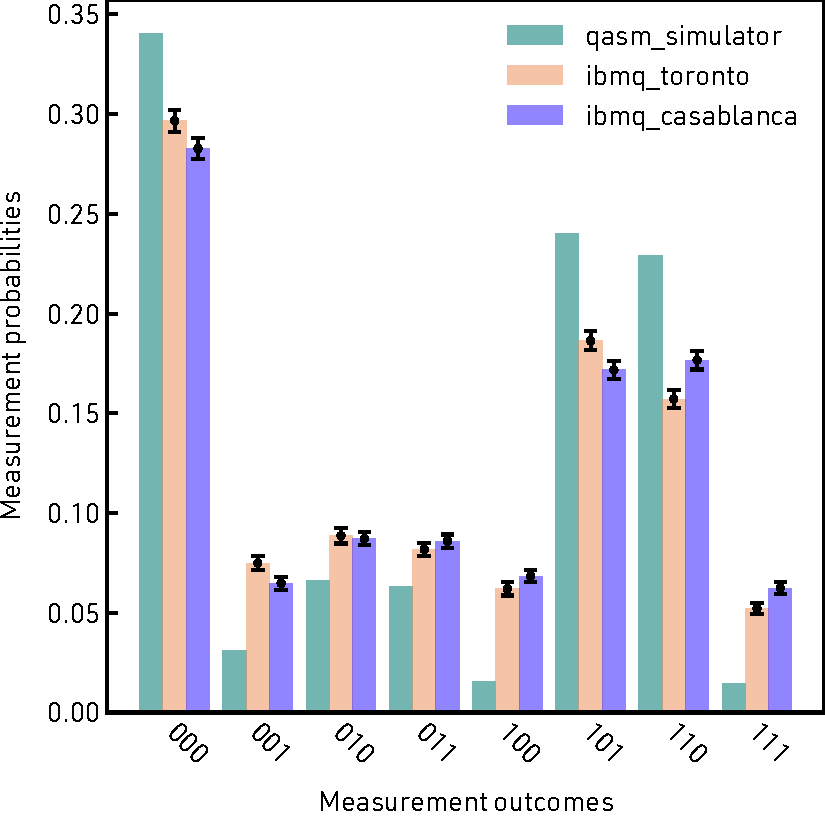
\includegraphics[width=0.86\textwidth]{shor_outcomes}
    \caption[Results of the complete quantum order-finding routine for ${N = 21}$ and ${x=4}$.]{Results of the complete quantum order-finding routine for ${N = 21}$ and ${x=4}$. On each processor, the circuit was executed ${8192 \times 100}$ times with measurement error mitigation. The error bars represent ${95\%}$ confidence intervals around the mean value of each histogram bin (see~\protect\refSectionOnly{error_bars} of technical~\protect\refAppendixOnly{appendix_B} details). The simulator probabilities show the ideal case.
    }
    \labelFigure{shor_outcomes}
\end{figure}

%p \begin{figure}[t!]
%     \centering
%     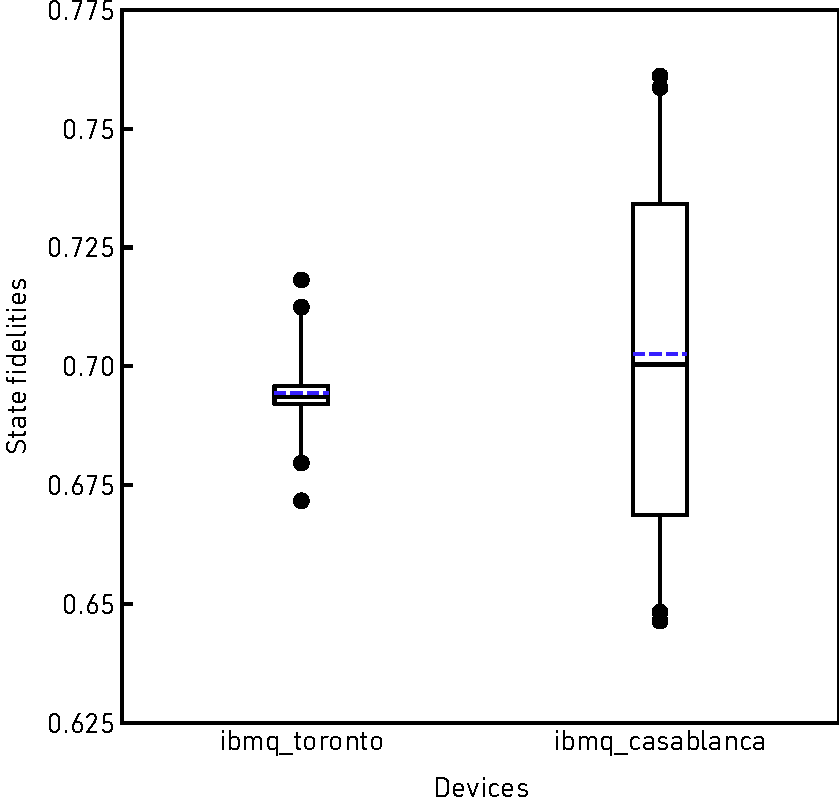
\includegraphics[width=0.90\textwidth]{shor_fidelities}
%     \caption[Boxplot of a sample ($\nu = 50$) of state fidelities from the respective two devices.]{Boxplot of a sample ($\nu = 50$) of state fidelities from the respective two devices showing the spread of the values around the sample mean and $95\%$ confidence intervals.}
%     \labelFigure{shor_box_plot}
% \end{figure}

\noindent
The theoretical ideal probability is close to $0.25$, as can be seen from the simulator results in~\refFigureOnly{shor_outcomes}. However, the amplification of the peaks $\ket{000}$, $\ket{101}$ and $\ket{110}$ is clearly visible from the processor outcomes. 

\bigskip
\noindent
We quantify the successful performance of the algorithm by comparing the experimental and ideal probability distributions \via the trace distance or Kolmogorov distance~\cite{Mike&Ike}, which measures the closeness of two discrete probability distributions $P$ and $Q$ and is defined by the equation $D(P,Q) \equiv \sum_{x \in \mathcal{X}}|P(x) - Q(x)|/2$, where ${\cal X}$ represents all possible outcomes. This measure shows an agreement between measured and ideal results -- the trace distance between the measured distribution and the ideal distribution is close to $0.1694$ and $0.1784$ for \textbf{ibmq\_toronto} and \textbf{ibmq\_casablanca}, respectively. On the other hand, the trace distance between the ideal distribution and a candidate random uniform distribution is $0.4347$. Furthermore, we evaluate the performance of the algorithm by characterizing the measured output state in the control register, this is achieved \via state tomography yielding the density matrix of the measured state. The measured state and ideal state on the output register are quantitatively compared using the fidelity for two quantum states $\varrho$ and $\var$, and is defined to be $F(\varrho, \varsigma) \equiv \Tr(\sqrt{\sqrt{\varrho}\varsigma\sqrt{\varrho}}^2)$~\cite{Mike&Ike}. We measured a fidelity of $F(\varrho_\text{id}, \varrho_{27Q})=0.6948 \pm 00650$ and $F(\varrho_\text{id}, \varrho_{7Q}) = 0.70 \pm 0.0275$ on the $27$ qubit and $7$ qubit quantum processors respectively. In~\refFigureOnly{shor_density_mats} we show the estimated density matrices in the computational basis for each respective device.

\clearpage

\begin{figure*}[t!]
    \centering
	\subfloat[\labelFigure{shor_mat2d_ideal_real}]
	{
		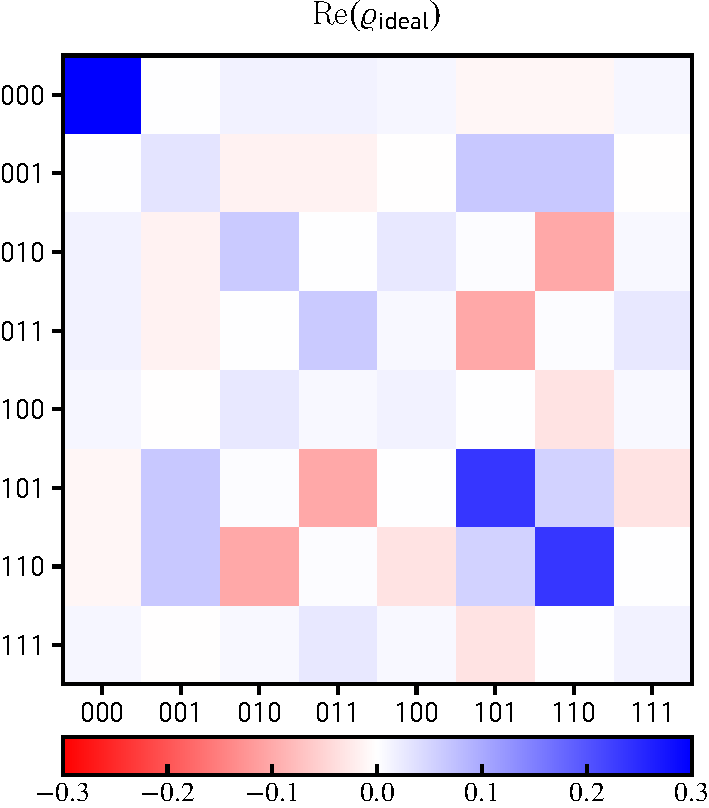
\includegraphics[width=0.5\textwidth]{shor_mat2d_ideal_real}
	}
	\subfloat[\labelFigure{shor_mat2d_ideal_imaginary}]
	{
		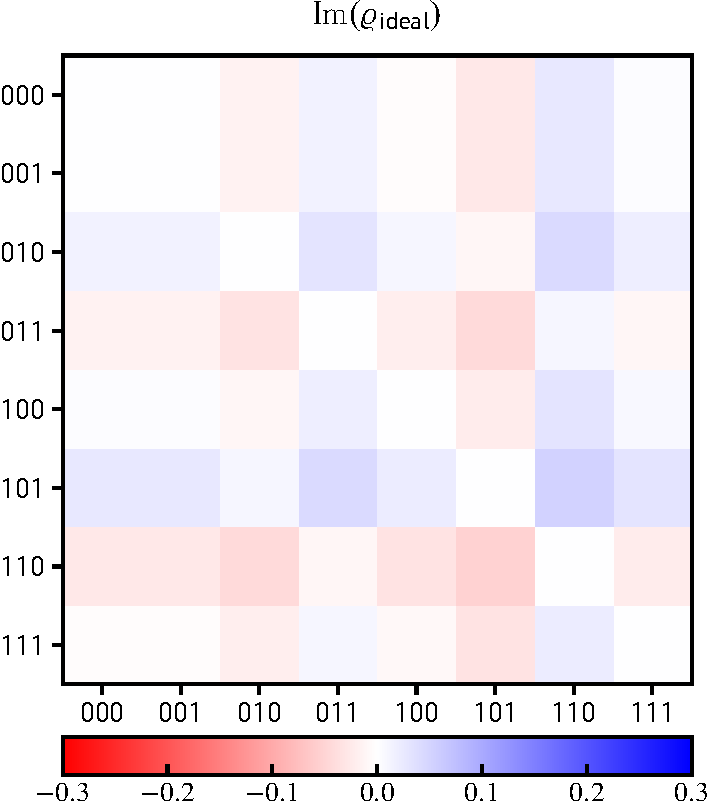
\includegraphics[width=0.5\textwidth]{shor_mat2d_ideal_imaginary}
	} \\
	\subfloat[\labelFigure{shor_mat2d_toronto_real}]
	{
		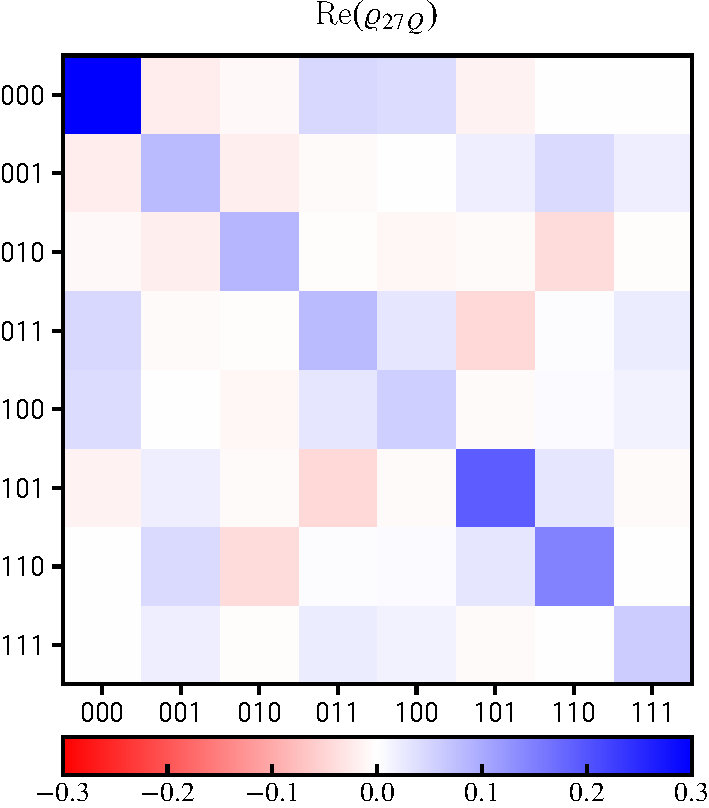
\includegraphics[width=0.5\textwidth]{shor_mat2d_toronto_real}
	}
	\subfloat[\labelFigure{shor_mat2d_toronto_imaginary}]
	{
		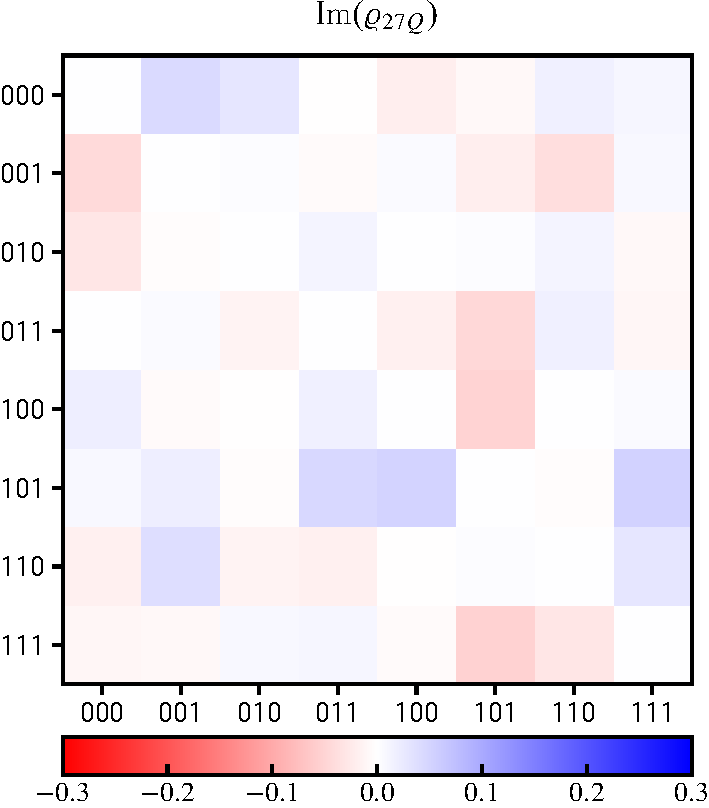
\includegraphics[width=0.5\textwidth]{shor_mat2d_toronto_imaginary}
	}
\end{figure*}

\clearpage

\begin{figure*}[t!]
	\addtocounter{subfigure}{4}
	\subfloat[\labelFigure{shor_mat2d_casablanca_real}]
	{
		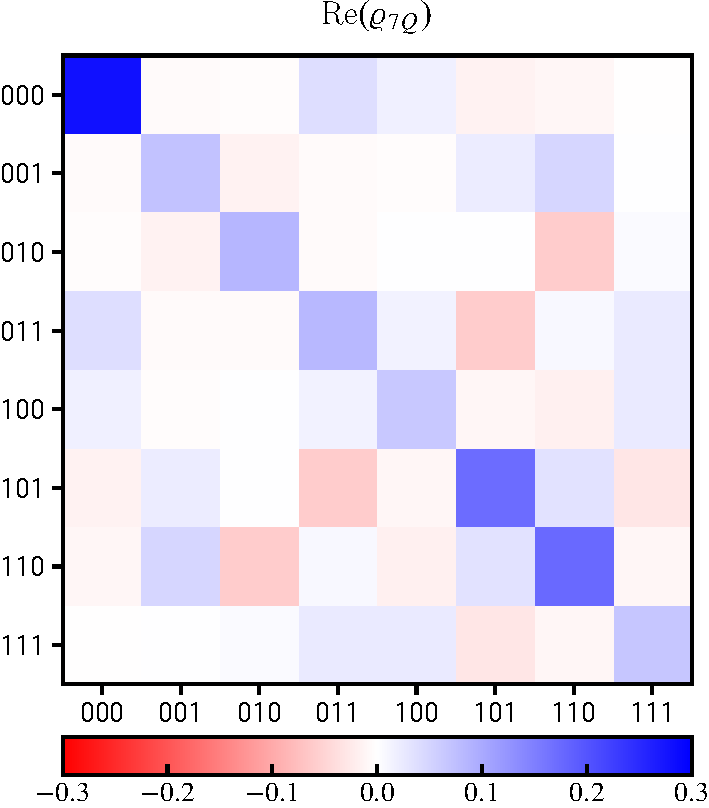
\includegraphics[width=0.5\textwidth]{shor_mat2d_casablanca_real}
	}
	\subfloat[\labelFigure{shor_mat2d_casablanca_imaginary}]
	{
		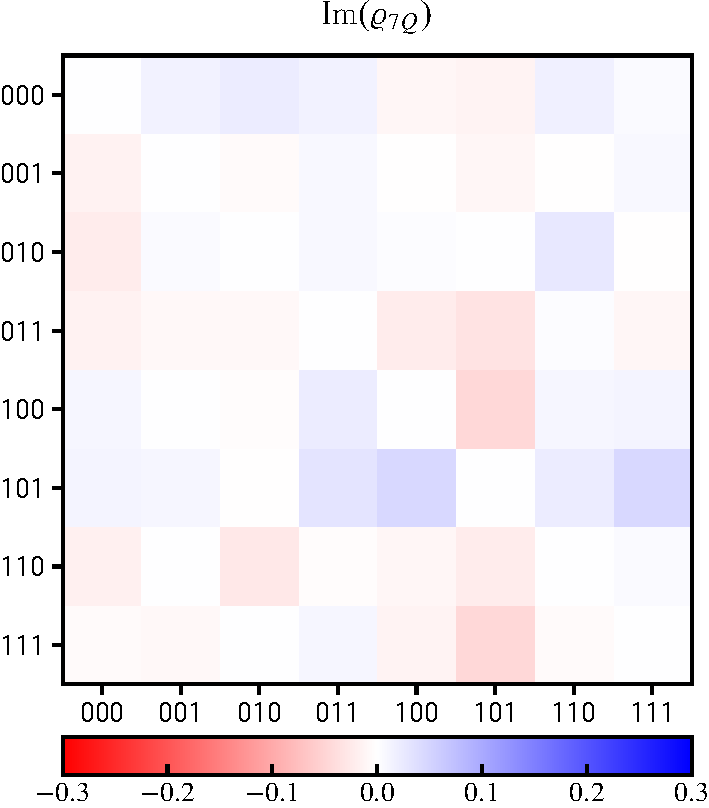
\includegraphics[width=0.5\textwidth]{shor_mat2d_casablanca_imaginary}
	}
    \caption[Ideal and measured density matrices after the inverse \acs{QFT}, estimated \via a maximum-likelihood reconstruction from measurement results in the Pauli-basis.]{Ideal and measured density matrices after the inverse \acs{QFT}, estimated \via a maximum-likelihood reconstruction from measurement results in the Pauli-basis. A matrix plot of the \textbf{(a)} real and \textbf{(b)} imaginary part of the ideal state $\op{\Psi}$. These plots are compared with the measured states $\rho_{27Q}$ and $\rho_{7Q}$ with the corresponding matrix plots of their real parts in panels \textbf{(c)} and \textbf{(e)}, and imaginary parts in panels \textbf{(d)} and \textbf{(f)}, respectively. We observe there is a resemblance between the ideal state and the measured states, but noise in both real and imaginary parts is notable. Note that in all figures the color bar has been rescaled to a range between $-0.3$ and $0.3$ for visual clarity.}
    \labelFigure{shor_density_mats}
\end{figure*}

\subsection{Factoring $N=21$}
\labelSection{C3_factoring_n_21}

The measured probability distributions in~\refFigureOnly{shor_outcomes} are peaked in probability for the outcomes $000~(\varphi_s=0)$, $101~(\varphi_s=5)$ and $110~(\varphi_s=6)$, with ideal probabilities of $0.35$, $0.25$ and $0.25$, respectively. Here we are using the integer representation of the binary outcomes. The outcome $000$ corresponds to a failure of the algorithm~\cite{Lopez_2012}. For the outcome $101$, computing the continued fraction expansion of $\varphi=\varphi_s/2^n=5/2^3=5/8$ gives the convergents $\{0, 1, 1/2, 2/3, 5/8\}$ (see~\refSectionOnly{continued_fractions} of  technical~\refAppendixOnly{appendix_B} for details), so that the third convergent $2/3$ in the expansion can be identified as $s/r$ and correctly gives $r=3$ as the order when tested with the relation $x^r \text{ mod } N=1$, while the other convergents do not give an $r$ that passes the test. On the other hand, the continued fraction expansion of $\varphi=6/8$ gives $\{0, 1, 3/4\}$ and incorrectly gives $r=4$ as the order (see~\refSectionOnly{continued_fractions} of technical~\refAppendixOnly{appendix_B} for details). This failure can be avoided in principle by adding further qubits to the control register so that the peak in the probability distribution becomes narrower and more well defined~\cite{Lopez_2012}. Another option is to simply apply continued fractions to all peaked outcomes and test if the value of $r$ found satisfies the order relation for $x$ and $N$. It is interesting to note that from the results of Ref.~\cite{Lopez_2012}, successfully finding the order $r=3$ was not possible to achieve, as with only two bits of accuracy in the experiment the continued fractions would always fail due to the peaked outcomes of $10~(2)$ and $11~(3)$ giving the convergents of $\{0,1/2\}$ and $\{0,1,3/4\}$, respectively. In our case, we successfully find $r=3$, from which we obtain $\gcd(x^{r/2}\pm1,N)=\gcd(8\pm1,21)=3$ and 7. Thus, with our demonstration, extending the number of outcome bits to three has allowed us to fully perform the quantum factoring of $N=21$.


%%%%%%%%%%%%%%%%%%%%%%%%%%%
%%%%%%%%%%%%%%%%%%%%%%%%%%%

\clearpage
\subsection{Verification of entanglement}
\labelSection{C3_verification_of_entanglement}

The presence of entanglement between the control and work registers is known to be a requirement for the algorithm to gain any advantageous speedup over its classical counterpart in general~\cite{Vidal_2003a, Braunstein_1999, Jozsa_2003}. For detecting genuine multipartite entanglement around the vicinity of an ideal state $\ket{\psi}$, one can construct a projector-based witness such as the one below:

\begin{align}
    \hat{\mathcal{W}}_{\psi} = \alpha \mathds{1} - \op{\psi}{\psi},
\end{align}

\noindent
where $\alpha$ is the square of the maximum overlap between $\ket{\psi}$ and all biseparable states. In other words, $\Tr(\hat{\mathcal{W}}_{\psi}\varrho) \geq 0$ for biseparable states and $\Tr(\hat{\mathcal{W}}_{\psi}\varrho) < 0$ for states with genuine multipartite entanglement in the vicinity of $\ket{\psi}$~\cite{Bourennane_2004}. For the ideal state after modular exponentiation (but before the inverse \acs{QFT}) in both the control and work registers, $\alpha=0.75$ was found using the method described in the appendix of Ref.~\cite{Bourennane_2004}. This was implemented using the software package QUBIT4MATLAB~\cite{Toth_2008}. Therefore ideally the state in both registers after modular exponentiation has genuine multipartite entanglement.

\bigskip
\noindent
In order to check whether the output state from the IBM processors is close to the ideal state and has genuine multipartite entanglement, full state tomography would normally be needed to characterize the state $\varrho_\text{exp}$ in both the control and work registers. This would require $3^5$ measurements, making it impractical to gather a sufficiently large data set within a meaningful time frame. However, we need not measure the full density matrix, the quantity $\Tr(\op{\Psi}{\Psi}\varrho_\text{exp})$ suffices. To measure this, we can decompose $\varrho=\op{\Psi}{\Psi}$ into $293$ Pauli terms as

\begin{align}
    \op{\Psi}{\Psi} = \displaystyle\sum_{ijklm} p_{ijklm} \sigma_i^{(1)}\sigma_j^{(2)}\sigma_k^{(3)}\sigma_l^{(4)}\sigma_m^{(5)},
\end{align}

\noindent
where $\sigma_{i} = \{I, X, Y, Z\}$ are the usual Pauli matrices plus the identity. 

\bigskip

\noindent
However, the number of measurements needed to obtain all 293 expectation values can be reduced. This is because the measured probabilities from a measurement of a single Pauli expectation value, \ie $\expval{ZZZZZ}$, can be summed in various combinations to derive other Pauli expectations values, \ie $\expval{ZIZZZ}, \expval{IZZZZ}$, etc. The values derived are nothing but the marginalization of the measured probabilities over the outcome space of some set of qubits (see~\refSectionOnly{pauli_measurements} of technical~\refAppendixOnly{appendix_B} for details). We can do the same for each term in the set of terms from the Pauli decomposition of $\varrho$, calling it $\mathcal{S}_d$, forming a set of other Pauli terms that can be derived from the same counts. Taking the union of these sets to be $\mathcal{S}_u$, the complement $\mathcal{S}_d\setminus\mathcal{S}_u$ gives the $79$ terms we only need to measure (see~\refSectionOnly{pauli_measurements} of technical~\refAppendixOnly{appendix_B} for details). We measure the 79 Pauli expectation values of the terms above with respect to the state in both registers after modular exponentiation and from this we compute/derive the $293$ terms in $\mathcal{S}_d$ and therefore $\Tr(\op{\Psi}{\Psi}\varrho_\text{exp})$; the measurement outcomes for evaluating some of the Pauli operator expectation values are shown in~\refFigureOnly{klocals}. 

\clearpage
\noindent
The measured probabilities for each term result in an expectation value of $\Tr(\op{\Psi}{\Psi}\varrho_{7Q}) = 0.677 \pm 0.00365$ and $\Tr(\op{\Psi}{\Psi}\varrho_{27Q}) = 0.626 \pm 0.00304$, which leads to

\begin{align}
  \Tr(\hat{\mathcal{W}}_{\Psi}\varrho_{7Q})  &= 0.0729 \pm 0.00365,\nonumber \\
  \Tr(\hat{\mathcal{W}}_{\Psi}\varrho_{27Q}) &= 0.124 \pm 0.00304.
\end{align}

\noindent
The results obviously fail to detect genuine multipartite entanglement, however, this does not mean entanglement is entirely absent. Consider the square of the maximum overlap between the ideal state $\ket{\Psi}$ and all pure states $\ket{\theta}$ that are unentangled product states with respect to some bipartite partition (bipartition) $\mathcal{B}$ of the qubits,

\begin{align}\labelEquation{maximal_overlap}
    \underset{\theta \in \mathcal{B}}{\max}{\abs{\ip{\theta}{\Psi}}^2} = \beta_{\Psi}.
\end{align}

\noindent
Thus, any other state $\ket{\xi}$ for which 

\begin{align}
    \abs{\ip{\xi}{\Psi}}^2 > \beta_{\Psi},
\end{align}

\noindent
cannot be a product state with respect to the bipartition $\mathcal{B}$, implying that there is non-separability, or entanglement, across this bipartition. The above result extends to mixed states $\varrho_\xi$ due to the convex sum nature of mixed quantum states~\cite{Toth_2008}. We compute \refEquationOnly{maximal_overlap} for all possible bipartitions of our ideal state $\ket{\Psi}$ (see~\refSectionOnly{maximum_overlap_wrt_bipartitions} of technical~\refAppendixOnly{appendix_B} for details). 

\bigskip
\noindent
For the experimental state $\varrho_{7Q}$ we find, with the exception of the bipartition $\mathcal{B}=(c_0c_1c_2q_1)(q_0)$, that it is non-separable with respect to all other bipartitions, \ie the square of the overlap between $\varrho_{7Q}$ and $\ket{\Psi}$ ($\sim 0.677$) is greater than the maximal square overlap between $\ket{\Psi}$ and all product states in each of these bipartitions. Similarly for $\varrho_{27Q}$, with the exception of bipartitions $\mathcal{B}=(c_0c_1c_2q_1)(q_0)$ and $\mathcal{B}=(c_0c_1c_2q_0)(q_1)$, the state is non-separable with respect to all other bipartitions. Most notably, both $\varrho_{7Q}$ and $\varrho_{27Q}$ are non-separable with respect to the bipartition ${\cal B}=(c_0c_1c_2)(q_0q_1)$, which is a bipartition between the control and work registers. 


% Another signature of non-separability between bipartitions of a pure state $\ket{\psi}$ is given by the entropy of entanglement~\cite{Bennett_1996},

% \begin{align}
% 	\mathcal{S}(\varrho_A) = -\tr(\varrho_a \log \varrho_A),
% \end{align}

% \noindent
% where $\varrho_A = \tr_B(\op{\psi})$ is the reduced density matrix of subsystem A of $\ket{\psi}$. If $\ket{\psi}$ is separable with respect to this bipartition, \ie $\ket{\psi} = \ket{\phi_A}\ket{\phi_B}$, then $\varrho_A = \op{\phi_A}$ is pure state for which the entropy of entanglement is $\mathcal{S}(\op{\phi_A}) = 0$; thus a non-zero entropy of entanglement indicative of non-separability between the two consideration bipartitions of $\ket{\psi}$.  We measure entropy of entanglement for our density matrix estimates (after the inverse \acs{QFT}) of the control register subsystem on each device, and find $\mathcal{S}(\varrho_{27Q}) = 1.659\pm0.0154$ $\mathcal{S}(\varrho_{7Q}) = 1.765\pm0.0387$,  respectively for the two devices.

% \bigskip
% \noindent
% This implies that non-separability or entanglement is present between the registers before (and after) the \acs{QFT}, as required for the algorithm's speedup in general~\cite{Vidal_2003a, Braunstein_1999, Jozsa_2003}. Furthermore, the maximum (not necessarily global but a good proxy of it) expectation value of the operator $\op{\Psi}{\Psi}$ for product states, is found \via a greedy search algorithm~\cite{Toth_2008} to be around $0.30$, further asserting that indeed the qubits are entangled with each other in some way.

\begin{figure*}[h!]
	\subfloat[\labelFigure{casablanca_klocals}]
	{
        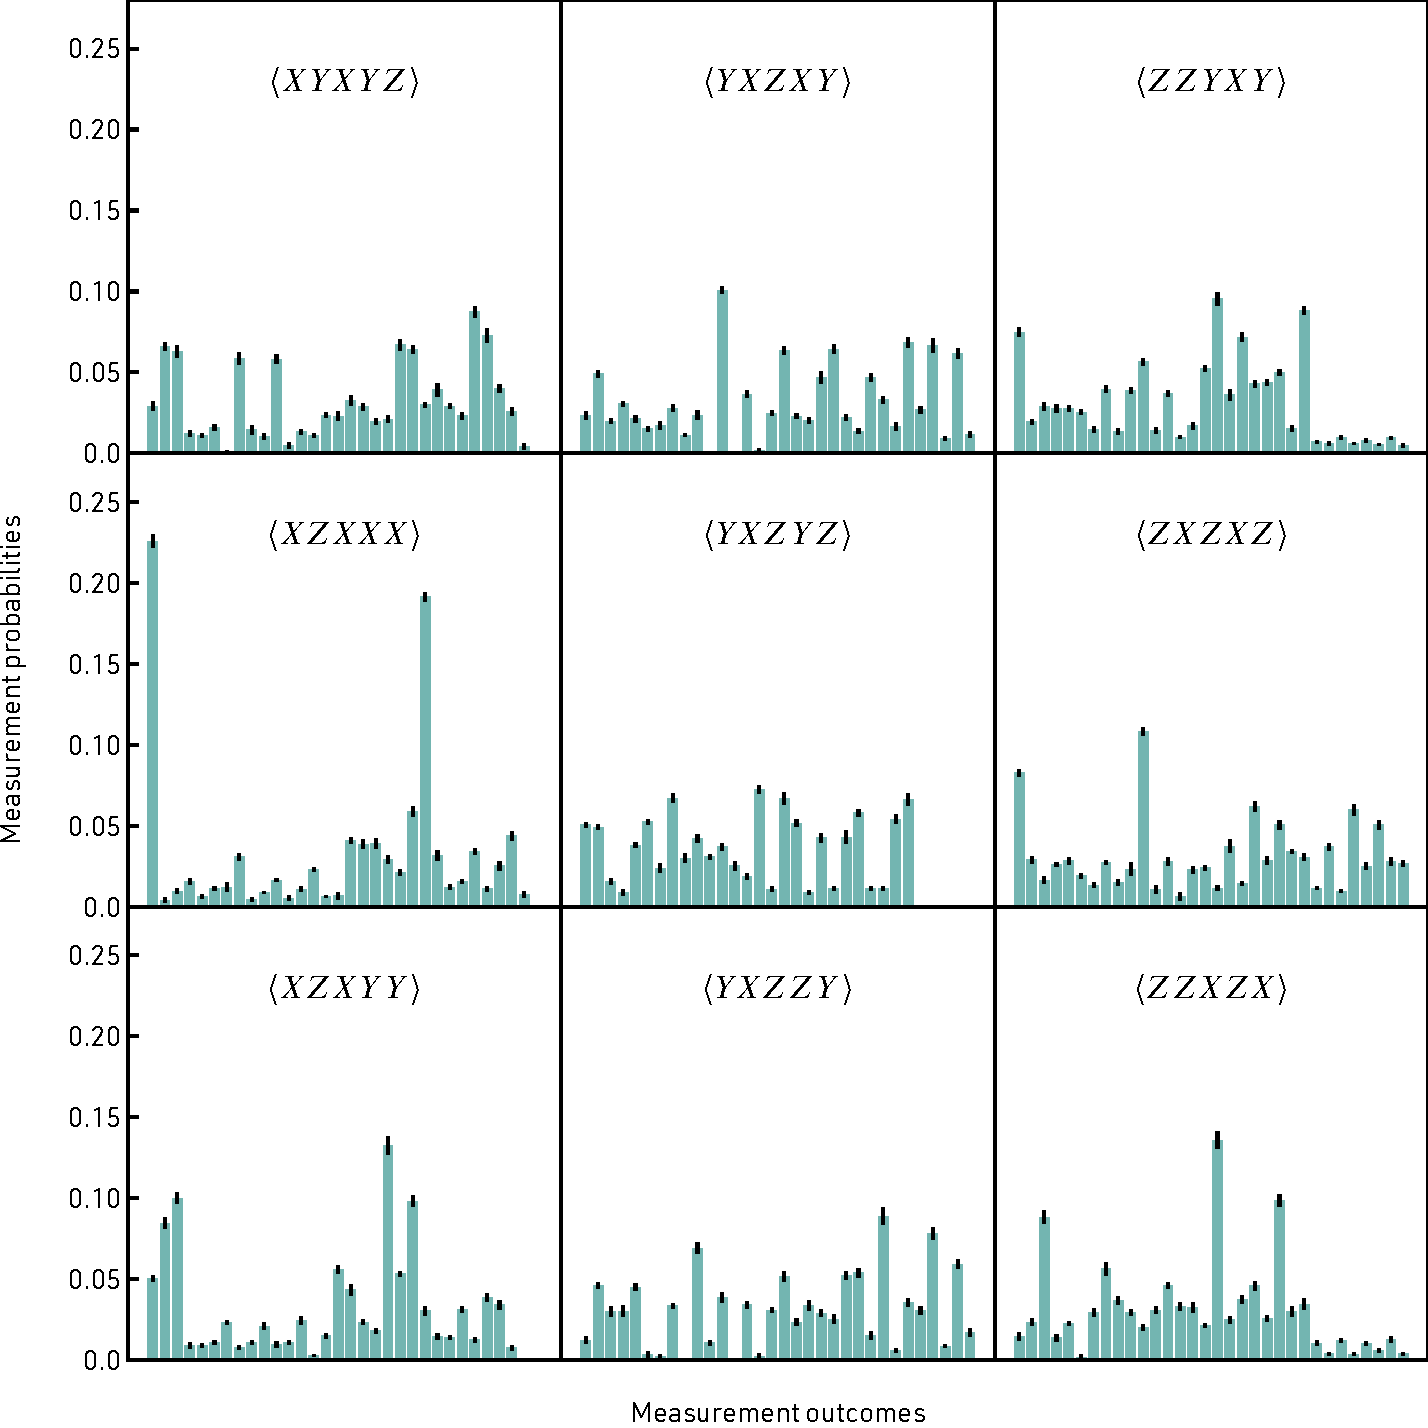
\includegraphics[width=\textwidth]{klocals_casablanca}
	}
\end{figure*}

\clearpage

\begin{figure*}[t!]
	\addtocounter{subfigure}{1}
	\subfloat[\labelFigure{toronto_klocals}]
	{
        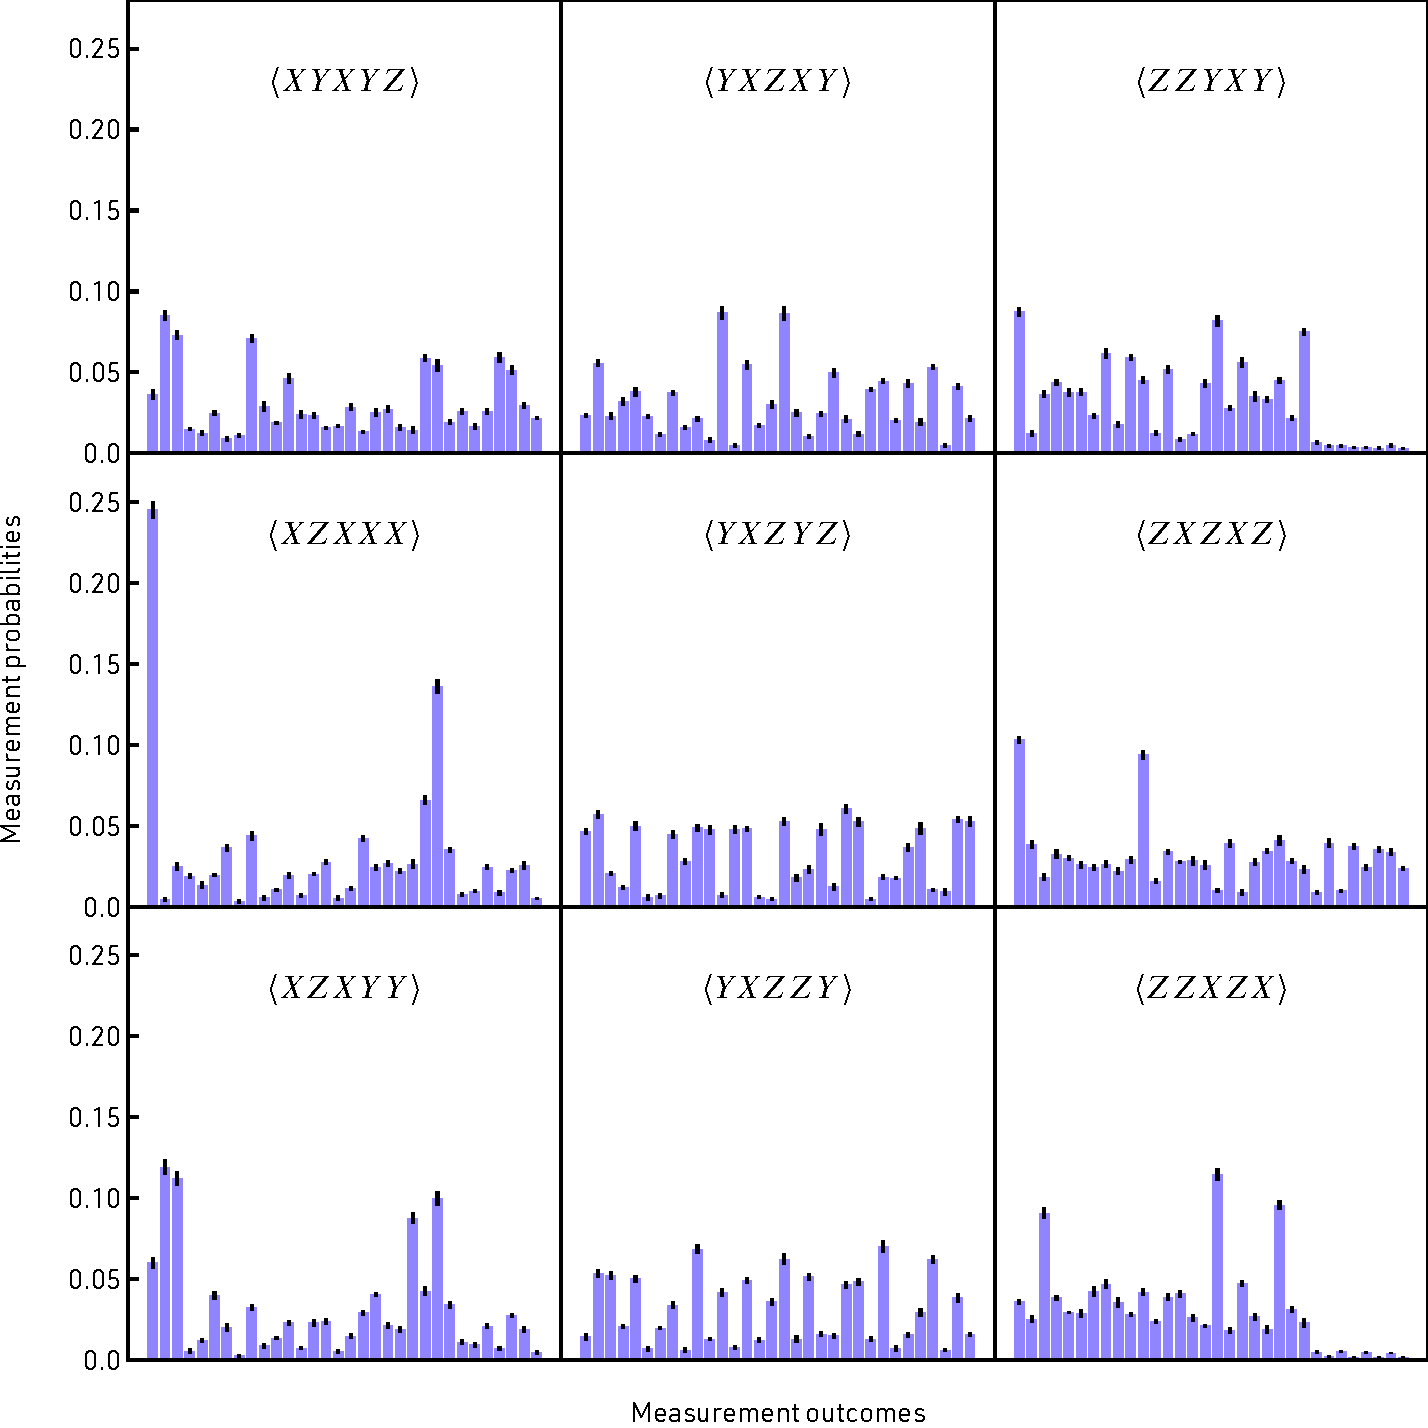
\includegraphics[width=\textwidth]{klocals_toronto}
	}
    \caption[A subset of 9 of the 79 measurement settings.]{A subset of 9 of the 79 measurement settings required for each term in: \textbf{(a)} $\Tr(\op{\Psi}{\Psi}\varrho_{7Q})$ and \textbf{(b)} $\Tr(\op{\Psi}{\Psi}\varrho_{27Q})$. The $x$-axis from left to right shows the labels from $p_{00000}$ to $p_{11111}$.}
    \labelFigure{klocals}
\end{figure*}

\clearpage

\section{Concluding remarks}
\labelSection{C3_concluding_remarks}
In summary, we have implemented a compiled version of Shor's algorithm on IBM's quantum processors for the prime factorization of $21$. By using relative phase shift Toffoli gates, we were able to reduce the resource demands that would have been required in the standard compiled and non-iterative construction of Shor's algorithm (with regular Toffoli gates), and still preserve its functional correctness. The use of relative phase shift Toffoli gates has also allowed us to extend the implementation in Ref.~\cite{Lopez_2012} to an increased resolution. Moreover, while the latter implementation used only 1 recycled qubit for the control register, in contrast to our 3 qubits, it falls one iteration short of achieving full factoring for the reasons already mentioned. It is not clear what additional resource overheads (single and two-qubit gates) would be needed in implementing another iteration in their scheme and it is likely that these overheads are what prevented the full factoring of 21 in the photonic setup used. Furthermore, we note that in principle there is no real advantage in using 3 qubits for the control register as we have done here instead of 1 qubit recycled, as in Ref.~\cite{Lopez_2012}. However, in practice it is not possible at present to recycle qubits on the IBM processors and so we used 3 qubits instead. In future, once this capability is added, a further reduction in resources will be possible for our implementation, potentially improving the quality of the results even more. 

\bigskip
\noindent
We have verified, \via state tomography, the output state in the control register for the algorithm, achieving a fidelity of around $0.70$. For the verification of entanglement generated during the algorithm's operation, the resource demands of state tomography were circumvented by measuring a much reduced number of Pauli measurements to directly estimate the fidelity of the state. However, this method is quite specialized and cannot be easily generalized to larger systems. In scaling up Shor's algorithm to higher integers beyond 21 using larger quantum systems, other methods of quantum tomography / direct fidelity estimation can be used to characterize the performance. These include compressed sensing~\cite{Gross_2010} and classical shadows~\cite{Huang_2020}, which give theoretical guarantees, and improved scaling in the number of Pauli measurements and classical post-processing than standard methods. In the case where one is only interested in a direct estimate of fidelity, the method due to Flammia and Liu~\cite{Flammia_2011} provides a fidelity estimate using a constant number of Pauli expectation values. 


\bigskip
\noindent
For states that belong to a class of states with certain symmetries, such as stabilizer states, only a few measurements are required for measuring the fidelity and detecting multipartite entanglement~\cite{Toth_2005}. However, not all entangled states are neatly housed within these well-studied classes. Ref.~\cite{Baccari_2017} introduces a device-independent method for multipartite entanglement detection which scales polynomially with the system size by relaxing some constraints. Another scheme constructs witnesses that require a constant number of measurements of the system size at the cost of robustness against white noise. This provides a fast and simple procedure for entanglement detection~\cite{Knips_2016}. Many fundamental questions on the subjects of quantum tomography and multipartite entanglement still remain to be answered~\cite{Banaszek_2013} and advances will help in efficiently quantifying the performance of algorithms in larger quantum processors.


\bigskip
\noindent
Our demonstration involves a two-fold reduction of the resource count from the full circuit in~\refFigureOnly{compiled_circ} \via the replacement of regular Toffoli gates with relative phase variants, which is an approach that is in the spirit of the NISQ era; tailoring quantum circuits to circumvent the shortcomings of noisy quantum processors. 

\clearpage
\noindent
 In addition, the resource count of the full \acs{QFT} in our circuit may be reduced through the use of the approximate \acs{QFT}~\cite{Barenco_1996}, while possibly still maintaining a clear resolution of the peaks in the output probability distribution~\cite{Coppersmith_2002}. A possible avenue of future research derived from what we have reported here is the investigation and identification of scenarios where one can replace Toffoli gates with relative phase Toffoli gates while preserving the functional correctness, in a wide range of algorithms including Shor's algorithm, as seen here. In the present case, whether such an approach is special to the case of $N=21$ or extendable to other $N$ is not known. Ref.~\cite{Maslov_2016} has performed some work in this regard, however a proper analysis and systematic composition of relative phase Toffoli gates for such purposes is still an open problem. In future, a similar approach may make possible the factorization of larger numbers with adequate accuracy in resolution of the algorithm's outcomes and their characterization.

%%%%%%%%%%%%%%%%%%%%%%%%%%%
%%%%%%%%%%%%%%%%%%%%%%%%%%%
%%%%%%%%%%%%%%%%%%%%%%%%%%%


\part{Building a three-qubit one-way quantum computer}
\labelPart{building_a_three_qubit_one_way_quantum_computer}

\chapter{Polarization-entangled photons}
\labelChapter{polarization_entangled_photons}

\begin{epigram}{\textit{Asher Peres, Quantum Theory: Concepts and Methods}}
    \enquote{Quantum phenomena do not occur in a Hilbert space. They occur in a laboratory.} 
\end{epigram}

\section{Introduction: Non-separability in the laboratory}
\labelChapter{C4_introduction}

\lettrine[lines=3]{I}{n} the introductory chapter we have described various linear optical elements and how information can be encoded and subsequently measured in the polarization \acs{DOF} of a single photon. As the avid reader (or by the title of this thesis) might have suspected, much of the appeal of such optical systems comes about from their potential applications to quantum information processing tasks. In this particular chapter, we steer towards this direction and consider this use of polarization-entangled pairs of photons generated \via a nonlinear process called \acs{SPDC}, with the polarization of a single-photon as a substrate for a quantum bit. Multi-qubit states that possess non-classical correlations have been realized in a variety of, and often exotic optical systems, but in this regard perhaps, the most readily available and controllable source of entanglement arises from polarization-entangled photons. This is in part attested by their ubiquitous use; for demonstrations of Shor's algorithm from the first half of thesis (see ~\refChapterOnly{quantum_prime_factorization}); after the pioneering work on a spin-$\nicefrac{1}{2}$ nuclei system~\cite{Vandersypen_2001}, have been realized on single-photonic architectures making use of polarized-entangled photons~\cite{Lu_2007,Lanyon_2007,Lopez_2012} and other sundry tasks; including state-preparation in measurement-based/one-way quantum computing~\cite{Lu_2006, Kiesel_2005, Park_2007, Vallone_2008, Tokunaga_2008}, algorithms~\cite{Walther_2005, Prevedel_2007, Chen_2007} and quantum communication protocols~\cite{Kiesel_2007, Gaertner_2008, Schmid_2010, Bell_2014}. 

\bigskip
\noindent
Needless to say, the commonality among all these demonstrations is the central role of entanglement, which necessitates the need for a complete characterization of such entangled states in such applications. In earlier pioneering work of this kind, qualitative arguments for the presence of entanglement were made in the way of violation of Bell-type inequalities from fringe visibility measurements being above a certain threshold~\cite{Kwiat_1995, Kwiat_1999}. Such measurements gave qualitative evidence for the existence of non-classical correlations in a given experiment, not consistent with any local hidden-variable theory~\cite{Bell_1964,CHSH_1969,GHZ_2007}. 

\bigskip
\noindent
A violation of Bell-type inequalities is often considered an excellence indicator of the presence of entanglement in a pure two-qubit system; alas, despite its experimental convenience, it is not a true measure of entanglement\footnote{Ref.~\cite{Munro_2001} shows that in general, it is not possible to discern the degree of entanglement (a quantifiable measure) in a state \via an inference from a violation of Bell-type inequality}. 

\clearpage
\noindent
A more thorough characterization of polarization-entangled photons is through \gls{QST}~\cite{Hradil_1997, James_2001}. From a set of measurements performed on an ensemble of identically prepared quantum states, a maximum likelihood estimate of the density matrix of the polarization-entangled photon state is obtained, and from which physical quantities of interest such as fidelity, purity and concurrence can be derived.

\section{Experimental design}
\labelSection{C4_experimental_design}

In the experiment that we will describe in this chapter, we endeavour to generate and characterize a photonic three-qubit maximally entangled state\footnote{Maximally entangled state has a maximum entropy of entanglement for each of its bipartitions. For a two qubits, the Bell states are examples of maximally-entangled states.} first studied by \gls{GHZ} and thus bears their name. The experimental procedure is conceptually simple to describe: A two-photon, two-qubit polarized-entangled state is generated from a \acs{SPDC} and appropriately characterized with quantum state tomography. Once characterized and optimized, this state is enlarged by using the path (momentum) \acs{DOF} of one of the photons to a three-qubit polarization and path entangled \acs{GHZ} state, locally equivalent to a graph state~\cite{Raussendorf_2003}. Encoding a quantum bit on a separate \acs{DOF} on one of the polarization-entangled photons is motivated by two main reasons.

\begin{itemize}
	\item[\emph{Primo}] Experimental convenience: Having additional photons (generated by another \acs{SPDC} process) in an experimental setup of this kind would necessitate additional tabletop linear optical components \ie mirrors, wave plates, beam splitters, filters, polarizers, etc. The end goal of the experiment is to eventually carry out remotely controllable measurements on the generated state, thus it is preferable to have fewer moving parts. 

	\item[\emph{Secondo}] Practicality: \acs{SPDC} is a probabilistic process, that is, for every photon incident on the crystal, with some probability $p$, it will down convert to a polarization-entangled photon-pair, and the probability $p$ is typically low, on the order of $\lesssim 1\%$~\cite{Kok_2007}. Thus having an additional two photons produced in our experimental setup would occur with even lower probability $p^2$ (assumption of independence of the two events), and would also alter the coincidence counting electronics; typically one has to allow a long coincidence window to observe multiple low probability events of this kind\footnote{In Ref.\cite{Lu_2006}, a six-photon, six-qubit polarized-entangled state was produced with three \acs{SPDC} processes occurring in succession,and six-fold coincidence events (${\sim p^3}$) were accumulated over a three hour coincidence window.}.
\end{itemize}

\noindent
Similarly, once this state is generated, we appropriately characterize it. Reconstructing the density matrix of a three-qubit state would necessitate a full tomographic analysis, which for a three-qubit state would require $64$ measurement settings~\cite{Resch_2005}. However, a \acs{GHZ} state is locally equivalent to another three-qubit state that is a member of a special class of states, called graph states~\cite{Hein_2004,Raussendorf_2003}. What is peculiar to graph states is that they are completely described by their so-called stabilizer operators, which provide an experimentally economical way to discern the presence of entanglement and a lower bound for the fidelity of the generated state by way of evaluating their expectation values~\cite{Toth_2005}.

\bigskip
\noindent
Once characterized, we proceed to automate the experimental calibration and measurement procedures. This is achieved by having the relevant linear optical components in our experimental setup, all connected to a centralized and remotely accessible server that mediates the control of the optical components. 

\clearpage

\begin{figure*}[t!]
  \centering
  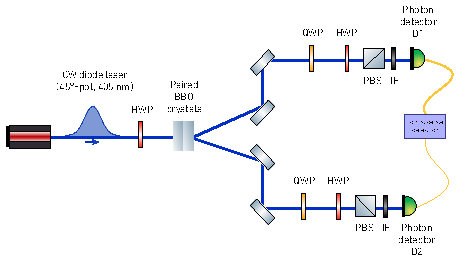
\includegraphics[width=1.0\textwidth]{experiment_1.pdf}%
  \caption[Experimental setup for generation and measurement of a two-photon two-qubit polarization-entangled Bell state.]{Experimental setup for generation and measurement of a two photon two-qubit Bell state. \gls{HWP}, \gls{QWP}, \gls{BBO}, \gls{PBS}, \gls{NPBS} and \gls{IF}. A photon pair is created whenever a laser pump photon with \SI{405}{nm} wavelength is incident on the paired \acs{BBO} crystals cut for type-I \acs{SPDC}, generating photons at \SI{810}{nm}. Each photon is guided by a set of mirrors to a \acs{QWP}, \acs{HWP}, and \acs{PBS} which are used to perform polarization measurements of the quantum state. Finally, each photon is sent to an \acs{IF} at \SI{800}{nm} with a bandwidth of \SI{40}{nm} and collected by a \gls{SMF} and sent to a photon detector. Each photon detector produces an electronic signal and sends it to the coincidence counting electronics, which count the signals that arrive simultaneously.}
  \labelFigure{experiment_1}
\end{figure*}

\noindent
With accessibility in mind, we designed a proof-of-concept mobile app that provides a graphical user interface to communicate with the server, which permits the user to specify an experiment with arbitrary (allowed) measurement settings and retrieve their experimental results. The rest of this chapter is dedicated to the filling in the details and describing the experimental design and subsequently, results from the experiments.

\bigskip
\noindent
The main goal of the initial stage of the experiment was to characterize the polarization-entangled two-photon two-qubit state from a \acs{SPDC} source using full quantum state tomography. To perform full quantum state tomography, we used the techniques and tools described in Ref.~\cite{James_2001}. We begin by describing the various components of the experimental apparatus shown in ~\refFigureOnly{experiment_1} --- A laser and \acs{SPDC} source, measurement apparatus, photon collection optics, and coincidence detection electronics. The \acs{SPDC} source used was two concatenated \SI{5}{\milli\meter} $\times$ \SI{5}{\milli\meter} $\times$ \SI{0.5}{\milli\meter} \gls{BBO} crystals cut for type-I phase matching, with their two optical axes aligned in perpendicular planes. 

\bigskip
\noindent
When this source is pumped with a vertically polarized pump beam, due to type-I phase-matching, down-conversion will occur in the first crystal producing  horizontally polarized energy-degenerate, non-collinear photon pairs. Similarly, a horizontally polarized pump beam will stimulate type-I down-conversion in the second crystal, generating energy-degenerate photon pairs. A diagonally polarized laser is likely to equally stimulate down-conversion in both crystals~\cite{Kwiat_1999}. Photons in the spatially overlapping regions, diametrically opposed (due to momentum conservation) on the two light cones, will be in the state $(\ket{H_1,H_2} + e^{i\phi}\ket{V_1,V_2})/\sqrt{2}$ as illustrated in~\refFigureOnly{two_type_I}. A main condition here is that the spatial modes of a given pair must have a significant overlap~\cite{Kwiat_1999}. Our \acs{SPDC} source is pumped with a \gls{CW} blue laser\footnote[][-55pt]{We keep our power relatively low, as high power pumps are known to stimulate double pair emissions~\cite{Weinfurter_2001,Fulconis_2007}, which degrade the single-photon quality. Our laser pump operates at a power of $\sim$\SI{50}{\milli\watt}) for every experiment we conducted unless stated otherwise.}, to produce frequency-degenerate photon pairs at a wavelength of \SI{810}{\nano\meter}, emitted onto a light cone with an (full) opening angle of $6^{\circ}$. 

\clearpage
\begin{figure}[h]
	\centering
	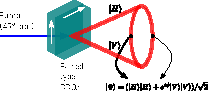
\includegraphics[width=\textwidth]{type-I-SPDC.pdf}
	\caption[Two paired \acs{BBO} ($\beta$-barium borate) crystals cut for type-I phase matching.][-15pt]{Two paired \acs{BBO} ($\beta$-barium borate) crystals cut for type-I phase matching as a source of entangled photons. For every pump photon, the photon pairs emerge from the crystal at a fixed from the pump photon thus creating a cone around the direction of the pump photon. Photon pairs at diametrically-opposed points where the cones intersect represent points of indistinguishability (spatial, temporal and polarizations), and their two-qubit state is an entangled state of the form shown in this figure. The $x$, $y$, $z$ axes are formed by the second crystal's optic axis, the pump beam and first crystal's optic axis respectively.}
	\labelFigure{two_type_I}
\end{figure}
\noindent
The value of $\phi$ is determined by the phase-matching, and details and geometry of the two crystals. The laser in our experiment produces vertically polarized light, we use a rotatable \acs{HWP}\footnote[][80pt]{Thorlabs Ø1/2" Mounted Zero-Order \acs{HWP} at \SI{405}{nm}} to adjust the beam to a desirable linear polarization.

\bigskip
\noindent
The next stage of the apparatus is dedicated for tomographic analysis of the experimentally generated state and detection. An arrangement of a rotatable \acs{QWP} and \acs{HWP}, and \acs{PBS}\footnote[][20pt]{Thorlabs Ø1/2" Mounted Zero-Order \acs{QWP}/\acs{HWP} at \SI{808}{nm} and PBS202 20 mm cube with wavelength range of \SI{620}-\SI{1000}{nm}, respectively.}, allows one to project any arbitrary polarization state. The \acs{IF}s are centred at \SI{800}{nm} with a \gls{FWHM} $\approx$ \SI{40}{nm} are used for spectral filtering, the photons in each output mode are then sent to a fibre coupler (FC)\footnote[][20pt]{With a Thorlabs RMS20X objective with an effective local length of \SI{9}{mm} and numerical aperture of $0.4$.} mounted on a Thorlabs MBT613D/M fibre launch with a FC-connectorized fibre holder with a \acs{SMF}\footnote[][20pt]{Thorlabs P1-830A-FC-5 \SI{5}{m} long fibre with cut-off wavelength range of \SI{830}-\SI{980}{nm}} directly coupled into a single photon detector - built-in silicon avalanche photo-diode (APD)\footnote[][20pt]{Excelitas single photon counting modules (SPCM), SPCM-AQRH-15 with efficiencies of 65\% and dark count rates of order $50s^{-1}$.}. These last two steps improve the spatial indistinguishability of the collected photons. The detector outputs go to a coincidence counting module described in detail in Ref.~\cite{Branning_2009}. An \gls{FPGA} board which takes inputs from the detectors, and outputs the signals and coincidences between the inputs into a computer serial port, accessed by a \textsf{LABVIEW} program, gives the experimenter data processing and storage capabilities. An \acs{FPGA} also permits a variable time window for $n$ input signals to be detected as an $n$-fold coincidence. In all the experiments presented, the coincidence window was set to $\sim$\SI{7}{ns}.

\section{A few practical notes on alignment}
\labelSection{C4_alignment}


The initial alignment stage was done with a lower-power class-1 red laser beam sent from the collection optics (fibre couplers) back towards the crystals. Using the 3-axis dials on the fibre launch and the two target irises\footnote[][20pt]{A more convenient, but less precise alignment technique uses two target rulers. Vertical alignment is achieved by directing the beam spot onto a target mark on both rulers. Horizontal alignment is achieved by having the beam spot clipped by the two rulers (which would be aligned by the screw holes on the optical table) equally.}, we could align the beam path precisely along the plane of the optical table. The beam path in either arm is directed towards a so-called Z-fold laser pattern, two-mirror arrangement. This two-mirror arrangement allows us to precisely get the two beams to be at the correct opening angles of the light cone from the \acs{BBO} crystals. By having a target with ruler markings at a distance $d$ from the \acs{BBO} crystals, we could get the two beams to have the correct distance from the \acs{CW} blue laser beam spot (measured on the target ruler) such that they are incident on the \acs{BBO} crystals close to the correct half-opening angle of $\theta/2 = 3^{\circ}$. A simplified schematic of this geometric arrangement is shown in~\refFigureOnly{crystal_geometry}. The furthest mirror from the \acs{BBO} crystals in the Z-fold arrangement aligns the red laser beam spot at the ruler target, and the other mirror aligns the red laser beam spot such that it is superimposed with the \acs{CW} blue laser beam spot on the \acs{BBO} crystals, the procedure is identical for the two arms.


\clearpage
\noindent
The above alignment procedure is precise enough such that when the two crystals are pumped with the \acs{CW} blue laser operating at $\sim$\SI{50}{\milli\watt} with the \acs{HWP} after it set to $22.5^{\circ}$ to stimulate both crystals, we can see a few coincidence counts when polarization tomographic analysis optics are set to project out the state $\ket{H_1,H_2}$. The angle is counterclockwise with respect to the fast axis inscribed on the mounted optic, which is aligned perpendicular to the plane of the optical table for the all wave-plates in our experiments. It is also worthy to mention that, all the mounted wave-plates should be oriented to be either front-facing or back-facing, such that a propagating beam is always incident on the optic on the same side. A mismatch of kind between two wave-plates would gives rise to $180^{\circ}$ relative difference between their optic axis, and as a consequence the reference frames for the polarization in the optic would be different.  A counterclockwise (from the front) tilt on a wave-plate for a beam propagating towards the front-face of the optic, appears as a clockwise tilt for a beam propagating in the opposite direction. Fine adjustments are done with the dials on the fibre couplers to maximize the coincidence counts for both the two-photon state $\ket{H_1, H_2}$ and $\ket{V_1,V_2}$ measurements, first independently then concurrently.



\begin{marginfigure}
	\centering
	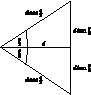
\includegraphics[width=.84\textwidth]{crystal_geometry.pdf}
	\caption[Schematic of the geometry due to the opening angle of the light cone from a \acs{SPDC} source.]{Schematic of the geometry due to the opening angle of the light cone from a \acs{SPDC} source; For a horizontal distance of $d$ from a \acs{SPDC} source, the two frequency-degenerate photons generated from the source will both be at a distance of $d\tan{\frac{\theta}{2}}$ from the horizontal axis, defined by the direction of original beam incident on the crystals.}
	\labelFigure{crystal_geometry}
\end{marginfigure}


\section{Results}
\labelSection{C4_results}
After we performed the coarse alignment procedure described above to a preliminary and satisfactory level, we performed full quantum state tomography for the two-photon, two-qubit polarization-entangled state with the theoretical machinery described by James \etal~\cite{James_2001}. We performed the full set of $16$ polarization measurement settings shown in~\refTableOnly{preliminary}. The coincidence rates were collected over a time interval of \SI{10}{s} for each measurement setting, with a coincidence window of \SI{7}{ns}. For the experimentally generated state $\varrho$,  for each measurement setting and corresponding projector in~\refTableOnly{preliminary}, experimentally we expect to observe the average number of coincidences given by $\nu_v = \expval{\psi_v}{\varrho}$. The set of projectors in the aforesaid table are complete set of measurements, that is, $\varrho$ can be completely and uniquely determined by the said set of measurements. From all $16$ projective measurements, it is possible to recover an estimate of $\varrho$.  Recover a valid density matrix estimate of $\varrho$ (Hermitian, positive etc) the estimate of $\varrho$ is recovered \via maximum likelihood (see~\cite{James_2001} for details). ~\refEquationOnly{preliminary_den} shows the reconstructed density matrix of the polarization entangled-state and~\refFigureOnly{preliminary} shows a graphical representation of this state. 

{
\begin{align}
	\varrho = \mqty(\
		0.43&-0.044-0.042i&0.021-0.061i&-0.14 + 0.32i \\
		-0.044+0.042i&0.013&0.016+0.0089i&-0.0071-0.024i \\
		0.021+0.061i&0.016-0.0892i&0.045&0.020+0.053i \\
		-0.14-0.32i&0.0071+0.024i&0.020-0.053i&0.51
	).
	\labelEquation{preliminary_den}
\end{align}
}

\noindent
The reconstructed state shows a commendable degree of entanglement; It has a fidelity of $F_{\varrho}=0.787\pm 0.0113$ with the maximally entangled state $(\ket{H_1,H_2} - i\ket{V_1,V_2})/\sqrt{2}$. Our measured state also achieves a value of $\ev{S} = 2.344+0.0228$ for the Bell-\acs{CHSH} operator, which represents a violation of the inequality, thus confirming that the state possess non-local correlations. Furthermore, from the density matrix, we can derive physical quantities that give an inkling of the statistical properties of the measured state. One such quantity is the linear entropy, which quantifies the statistical \enquote{mixedness} of the measured state. We measure it to have a value of $S_L= 4/3(1 - \Tr(\varrho^2)) = 0.387+0.0183$. 

\clearpage

\begin{table}[h]
	\centering
	\caption[Measurement settings and coincidence counts for a preliminary tomography analysis of a two-photon polarization state prior to optimization.][6pt]{Measurement settings and coincidence counts for a preliminary tomography analysis of a two-photon polarization state prior to optimization. Coincidence counts, collected over a ten second intervals, for each of the $16$ settings, are sufficient to recover an estimate of the density matrix of the two-qubit polarization state of the two photons. Here, ${\ket{D}\defeq(\ket{H}+\ket{V})/\sqrt{2}}$, ${\ket{L}\defeq(\ket{H}+i\ket{V})/\sqrt{2}}$ and ${\ket{R}\defeq(\ket{H}-i\ket{V})/\sqrt{2}}$}
	\labelTable{preliminary}
	\begin{tabular}{llllllll}
		\toprule
		$m$ & Projector & $h_1$ & $q_1$ & $h_2$ & $q_2$ & $N$ ($10s^{-1}$) \\
		\toprule
		$1$  & $\op{V}\otimes\op{V}$ & $45^{\circ}$   & $0^{\circ}$  & $45^{\circ}$    & $0^{\circ}$   & 2348 \\
		$2$  & $\op{V}\otimes\op{H}$ & $45^{\circ}$   & $0^{\circ}$  & $0^{\circ}$     & $0^{\circ}$   & 24 \\
		$3$  & $\op{H}\otimes\op{H}$ & $0^{\circ}$    & $0^{\circ}$  & $0^{\circ}$     & $0^{\circ}$   & 2410 \\
		$4$  & $\op{H}\otimes\op{V}$ & $0^{\circ}$    & $0^{\circ}$  & $45^{\circ}$    & $0^{\circ}$   & 206 \\
		$5$  & $\op{L}\otimes\op{V}$ & $22.5^{\circ}$ & $0^{\circ}$  & $45^{\circ}$    & $0^{\circ}$   & 720 \\
		$6$  & $\op{L}\otimes\op{H}$ & $22.5^{\circ}$ & $0^{\circ}$  & $0^{\circ}$     & $0^{\circ}$   & 1295 \\
		$7$  & $\op{D}\otimes\op{H}$ & $22.5^{\circ}$ & $45^{\circ}$ & $0^{\circ}$     & $0^{\circ}$   & 1525 \\
		$8$  & $\op{D}\otimes\op{V}$ & $22.5^{\circ}$ & $45^{\circ}$ & $45^{\circ}$    & $0^{\circ}$   & 1346 \\
		$9$  & $\op{D}\otimes\op{L}$ & $22.5^{\circ}$ & $45^{\circ}$ & $22.5^{\circ}$  & $0^{\circ}$   & 2350 \\
		$10$ & $\op{D}\otimes\op{D}$ & $22.5^{\circ}$ & $45^{\circ}$ & $22.5^{\circ}$  & $45^{\circ}$  & 1005 \\
		$11$ & $\op{L}\otimes\op{D}$ & $22.5^{\circ}$ & $0^{\circ}$  & $22.5^{\circ}$  & $45^{\circ}$  & 2132 \\
		$12$ & $\op{V}\otimes\op{D}$ & $45^{\circ}$   & $0^{\circ}$  & $45^{\circ}$    & $45^{\circ}$  & 826 \\
		$13$ & $\op{H}\otimes\op{D}$ & $0^{\circ}$    & $0^{\circ}$  & $0^{\circ}$     & $45^{\circ}$  & 1705 \\
		$14$ & $\op{H}\otimes\op{R}$ & $0^{\circ}$    & $0^{\circ}$  & $0^{\circ}$     & $90^{\circ}$  & 1129 \\
		$15$ & $\op{V}\otimes\op{R}$ & $45^{\circ}$   & $0^{\circ}$  & $45^{\circ}$    & $90^{\circ}$  & 1662 \\
		$16$ & $\op{L}\otimes\op{R}$ & $22.5^{\circ}$ & $0^{\circ}$  & $22.5^{\circ}$  & $90^{\circ}$  & 626 \\
		\toprule
	\end{tabular}
\end{table}

\begin{figure}[h]
    \centering
	\subfloat[\labelFigure{preliminary_re}]
	{
        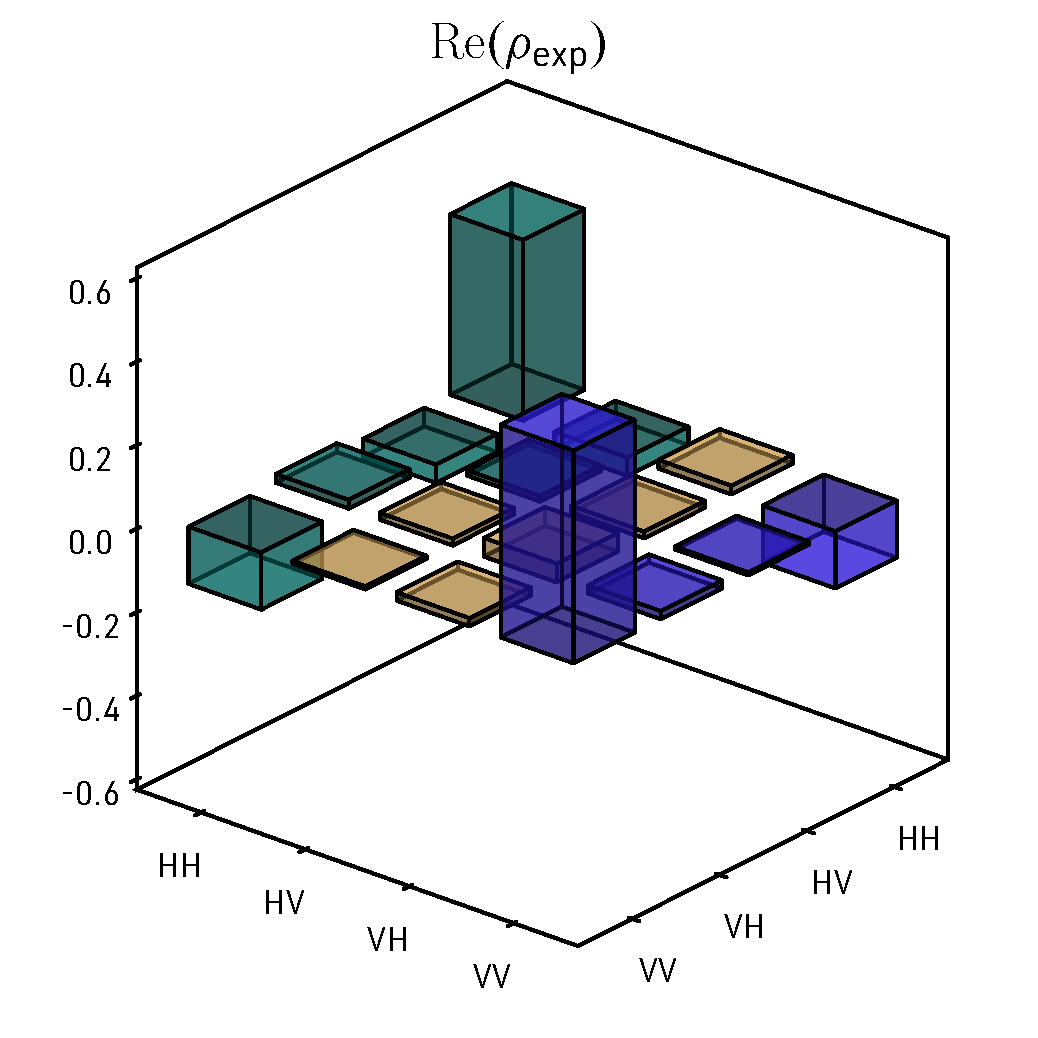
\includegraphics[width=0.5\textwidth]{preliminary_EPR_den_mat_Re.pdf}
	}
	\subfloat[\labelFigure{preliminary_im}]
	{
        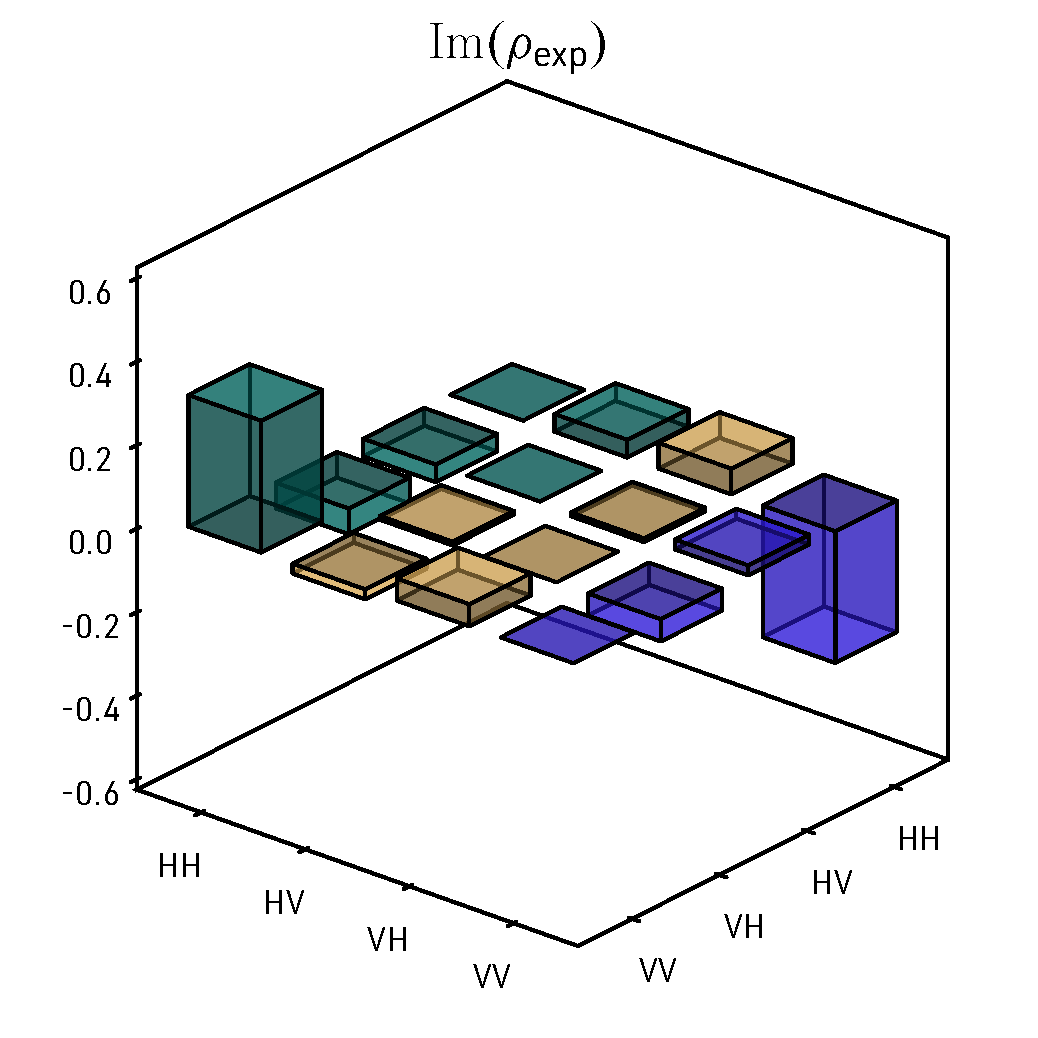
\includegraphics[width=0.5\textwidth]{preliminary_EPR_den_mat_Im.pdf}
	}
	\caption[Density matrix of a state estimated by maximum likelihood tomography from experimental data prior to optimization.]{Density matrix of a state estimated by maximum likelihood tomography prior to optimization, from the experimental data given in~\protect\refTableOnly{preliminary} \textbf{(a)} Real part of the estimate of $\varrho$. \textbf{(b)} Imaginary part of the estimate of $\varrho$.}
	\labelFigure{preliminary}
\end{figure}

\noindent
As also reflected by the graphical representation of the density matrix of this state, this value indicates a considerable amount of mixture present in measured state. The errors of the quantities here were also estimated from a Monte Carlo simulation of $100$ samples with Poisson noise. The values for quantities reported above are not necessarily of low quality; the generated state shows a fidelity of commendable quality, and significant degree of entanglement. However, we had to a reason to suspect that the state generated could be improved. An experiment of a similar kind~\cite{Kwiat_1999}, reports over $140$ coincidence counts per second per milliwatt of pump power over a \SI{5}{\nano\meter} bandwidth and a value of $\ev{S} = 2.700$, thus there is much room for improvement.

\bigskip
\noindent
Next we will describe the optimization procedure followed to improve the quality of the state generated in the experiment, and the subsequent result. Optimization is with respect to some utility function, and what will be described here is not necessarily a procedure suitable in all circumstances, and definitively imperfect. An imperative of uttermost practical importance to our experiment, was the tuning of the value of $\phi$ in the state $\ket{H_1,H_2} + e^{i\phi}\ket{V_2,V_2}$ generated by the \acs{SPDC} source. 

\clearpage
\noindent
As it can be inferred from the preliminary results, for that particular state, which has a significant fidelity with the state $\ket{H_1,H_2} - i\ket{V_1,V_2}$, the value of $\phi$ can be crudely inferred to take on a value $\phi=\pi$. We seek to generate one of the four Bell states:

\begin{align}
	\labelEquation{bell_states}
	\ket{\Phi^+}   &= \frac{1}{\sqrt{2}} \left(\ket{H_1,H_2} + \ket{V_1,V_2}\right), \nonumber \\
	\ket{\Phi^-}   &= \frac{1}{\sqrt{2}} \left(\ket{H_1,H_2} - \ket{V_1,V_2}\right),\nonumber \\
	\ket{\Psi^{+}} &= \frac{1}{\sqrt{2}} \left(\ket{H_1,V_2} + \ket{V_1,H_2}\right), \nonumber \\
	\ket{\Psi^{-}} &= \frac{1}{\sqrt{2}} \left(\ket{H_1,V_2} - \ket{V_1,H_2}\right).
\end{align}

\noindent
This imperative is once again motivated by the end goal of ultimately generating a three qubit \acs{GHZ} state. Thus, with this end in view, it is more experimentally convenient if we were to generate either one of the first two Bell states in~\refEquationOnly{bell_states}. In any case, our \acs{SPDC} source alone is limited to the generation of these two particular Bell states\footnote[][-10pt]{All four Bell states are equivalent up to some local unitary operation, for instance, if our \acs{SPDC} source generates the states $\ket{H_1,H_2}\pm\ket{V_1,V_2}$, an extra \acs{HWP} in the second arm that interchanges $H$ and $V$ (rotated $45^{\circ}$ counterclockwise to its fast-axis), prepares $\ket{H_1,V_2}\pm\ket{V_1,H_2}$. Similarly, the unitary operator $U = \mathds{1} \otimes S$, where $S=\diag(1, i)$, acting on $\ket{H,H}\pm i\ket{V_1,V_1}$, prepares $\ket{H_1,H_2}\pm\ket{V_1,V_1}$.}. We chose to optimize for the second Bell state, the optimization procedure for this particular state is guarded by the following observations.

\bigskip
\noindent
Consider one of the projectors from tomography analysis, $P_{DD} = \op{D_1}\otimes\op{D_2}$ where $\ket{D} = (\ket{H} + \ket{V})/\sqrt{2}$. Calculating the expectation value of the projector\footnote[][40pt]{This expectation value is related to the probability of a getting an outcome associated with the projector upon performing the projective measurement on $\ket{\Phi^{-}}$.} with respect to the state $\ket{\Phi^{-}}$ in ~\refEquationOnly{bell_states}, we observe that (omitting normalization constants):

\begin{align}
	\labelEquation{obs_1}
	&\ev{P_{DD}}{\Phi^{-}} = \ev{(\ketbra{D_1}{D_1} \otimes \
	\ketbra{D_2}{D_2})}{\Phi^{-}} \nonumber, \\
	&=\abs{\bra{H}\ket{D}}^4 - \
	\abs{\braket{D}{H}\braket{V}{D}}^2 - \
	\abs{\braket{D}{H}\braket{V}{D}}^2 + \
	\abs{\bra{V}\ket{D}}^4 \nonumber ,\\
	&= \left(\frac{1}{\sqrt{2}}\right)^4 - \left(\frac{1}{\sqrt{2}}\right)^4 - \left(\frac{1}{\sqrt{2}}\right)^4 + \left(\frac{1}{\sqrt{2}}\right)^4 \nonumber ,\\
	&= 0.
\end{align}

\noindent
Similarly, the projector $P_{LR} = \op{L_1}\otimes\op{R_2}$, where $\ket{L/R} = (\ket{H} \pm i \ket{V})/\sqrt{2}$ gives:

\begin{align}
	\labelEquation{obs_2}
	&\ev{P_{LR}}{\Phi^{-}} = \ev{(\ketbra{L_1}{L_1} \otimes \
	\ketbra{R_2}{R_2})}{\Phi^{-}} \nonumber, \\
	&=\abs{\braket{H}{L} \braket{R}{H}}^2 - \
	\braket{H}{L}\braket{L}{H}\braket{H}{R}\braket{R}{V} \nonumber, \\
	&\quad-\braket{V}{L}\braket{L}{H}\braket{V}{R}\braket{R}{H} + \
	\abs{\braket{V}{L} \braket{R}{V}}^2 \nonumber, \\
	&= \left(\frac{1}{\sqrt{2}}\right)^4 - \left(\frac{1}{\sqrt{2}}\right)^4 - \left(\frac{1}{\sqrt{2}}\right)^4 + \left(\frac{1}{\sqrt{2}}\right)^4 \nonumber, \\
	&= 0. 
\end{align}

\noindent
Aided by the above observations, we conjure up a procedure to optimize for the state $\ket{\Phi^-}$:

\begin{itemize}
	\item[\emph{Primo}] Set the polarization analysis optics to project out $\ket{H_1,H_2}$ and maximize the corresponding coincidence counts, typically achieved by fine adjustments to using the $z$-dial on the kinematic mount that holds the \acs{BBO} crystals, which tilts the crystals with respect to the $z$-$x$ plane (left-handed Cartesian coordinate system). Similarly, maximize the coincidence counts for the projection of $\ket{V_1,V_2}$, achieved by fine adjustments to the dials on the rotation stage at the bottom of the kinematic mount, which rotate the crystals about to the $z$-axis. \item[\emph{Secondo}] Set the polarization analysis optics to project out $\ket{D_1,D_2}$ and minimize the corresponding coincidence counts, which we achieved by rotating the crystals with respect to $y$-axis with the radial dial on the kinematic mount. Similarly, set the polarization analysis optics to project out $\ket{L_1,R_2}$ and minimize the corresponding coincidence counts, by using the $x$-$y$ axis dials on either side of the kinematic mount.
	\item[\emph{Terzo}] We go through several iterations of this process, and roughly equalize the two coincidence counts observed for $\ket{H_1,H_2}$ and $\ket{V_1,V_2}$, while minimizing the ones observed for $\ket{D_1,D_2}$ and $\ket{L_1,R_2}$.
\end{itemize}

\noindent
While iterating the steps of the above procedure, one eventually reaches a point where additional iterations have non-desirable results; The coincidence counts for $\ket{D_1,D_2}$ and $\ket{L_1,R_2}$ reach some local minimum (typically around $30s^{-1}$) and start increasing again, or the counts for $\ket{H_1,H_2}$ and $\ket{V_1,V_2}$ are no longer equal. At this point we halt and take the previous iteration to be optimal. Physically, the optimization procedure is changing the opening directions of the two light cones emerging from the \acs{BBO} crystals such that the collection optics in our experiment can access as much of the light cones as possible, and as close as possible to diametrically-opposed regions of indistinguishability. The measurement results after several iterations of this process are shown in ~\refTableOnly{tomo_analysis} and the corresponding graphical representation of the reconstructed density matrix shown in~\refFigureOnly{2q_tomo}, where the corresponding density matrix for the two-photon state is given by

\begin{align}
	\labelEquation{epr_density}
	\varrho = \mqty(
		0.49&0.028+0.033i&0.017-0.025i&-0.41+0.054i \\
		0.028-0.033i&0.0074&-0.0019+0.0017i&0.0011+0.023i \\
		0.017+0.025i&-0.0019-0.0017i&0.0074&-0.034-0.042i \\
		-0.41-0.054i&0.0011-0.023i&-0.034+0.042i&0.49 \\
	).
\end{align}

\noindent
From the above density matrix and its graphical representation, in comparison to the earlier reconstruction in ~\refFigureOnly{preliminary}, we note a few conspicuous differences. The populations of horizontally-and vertically-polarized photons are equalized in the optimized measured state\footnote[][-10pt]{Represented by the diagonal element on the top-left and diagonal element bottom-right respectively.}.  Likewise, the coherences\footnote[][20pt]{Represented by the off-diagonal elements. For this particular instance, the entries on the bottom left and top right.} between these two populations are equalized, and have a close resemblance to the coherences of the Bell state $\ket{\Phi^{-}}$; the fidelity between the measured state and the aforementioned state is $F_\varrho=0.902 \pm 0.00588$. Furthermore, there is an improvement of the other previously reported physical quantities; The measured state a violates a Bell-\acs{CHSH} inequality, attaining a value of $\ev{S} = 2.594\pm0.0153$. 

\bigskip
\noindent
Lastly, the linear entropy of the above state has a value of $S_L=0.211\pm0.0134$, which reflects a decrease in the \enquote{mixedness} of the state, in comparison to the earlier reconstruction. The errors in these quantities were estimated from a Monte Carlo simulation of $100$ samples with Poissonian noise on the count statistics\footnote[][-40pt]{This is because due to the probabilistic nature of \acs{SPDC}, the number of $n$ discrete photon pairs that arrive at the detectors for given a collection time interval $\Delta t$ follows a Poissonian probability distribution $\text{Pois}(\lambda = n \Delta t)$.}.

\clearpage

\begin{table}[t!]
	\centering
	\caption[Measurement settings and doublce coincidence counts for a tomography analysis of a two-photon polarization state after optimization.][6pt]{Measurement settings and coincidence counts for a tomography analysis of a two-photon polarization state after optimization. Coincidence counts, collected over a ten second intervals, for each of the $16$ settings, are sufficient to recover an estimate of (reduced) density matrix of the two-qubit polarization state of the two photons. Here, ${\ket{D}\defeq(\ket{H}+\ket{V})/\sqrt{2}}$, ${\ket{L}\defeq(\ket{H}+i\ket{V})/\sqrt{2}}$ and ${\ket{R}\defeq(\ket{H}-i\ket{V})/\sqrt{2}}$.}
	\labelTable{tomo_analysis}
	\begin{tabular}{llllllll}
		\toprule
		$m$ & Projector & $h_1$ & $q_1$ & $h_2$ & $q_2$ & $N$ ($10s^{-1}$) \\
		\toprule
		$1$  & $\op{V}\otimes\op{V}$ & $45^{\circ}$   & $0^{\circ}$  & $45^{\circ}$    & $0^{\circ}$   & 2738(83) \\
		$2$  & $\op{V}\otimes\op{H}$ & $45^{\circ}$   & $0^{\circ}$  & $0^{\circ}$     & $0^{\circ}$   & 33(5) \\
		$3$  & $\op{H}\otimes\op{H}$ & $0^{\circ}$    & $0^{\circ}$  & $0^{\circ}$     & $0^{\circ}$   & 2718(69) \\
		$4$  & $\op{H}\otimes\op{V}$ & $0^{\circ}$    & $0^{\circ}$  & $45^{\circ}$    & $0^{\circ}$   & 35(2) \\
		$5$  & $\op{L}\otimes\op{V}$ & $22.5^{\circ}$ & $0^{\circ}$  & $45^{\circ}$    & $0^{\circ}$   & 1256(14) \\
		$6$  & $\op{L}\otimes\op{H}$ & $22.5^{\circ}$ & $0^{\circ}$  & $0^{\circ}$     & $0^{\circ}$   & 1492(40) \\
		$7$  & $\op{D}\otimes\op{H}$ & $22.5^{\circ}$ & $45^{\circ}$ & $0^{\circ}$     & $0^{\circ}$   & 1470(23) \\
		$8$  & $\op{D}\otimes\op{V}$ & $22.5^{\circ}$ & $45^{\circ}$ & $45^{\circ}$    & $0^{\circ}$   & 1479(26) \\
		$9$  & $\op{D}\otimes\op{L}$ & $22.5^{\circ}$ & $45^{\circ}$ & $22.5^{\circ}$  & $0^{\circ}$   & 1434(46) \\
		$10$ & $\op{D}\otimes\op{D}$ & $22.5^{\circ}$ & $45^{\circ}$ & $22.5^{\circ}$  & $45^{\circ}$  & 284(15) \\
		$11$ & $\op{L}\otimes\op{D}$ & $22.5^{\circ}$ & $0^{\circ}$  & $22.5^{\circ}$  & $45^{\circ}$  & 1614(31) \\
		$12$ & $\op{V}\otimes\op{D}$ & $45^{\circ}$   & $0^{\circ}$  & $45^{\circ}$    & $45^{\circ}$  & 1549(31)\\
		$13$ & $\op{H}\otimes\op{D}$ & $0^{\circ}$    & $0^{\circ}$  & $0^{\circ}$     & $45^{\circ}$  & 1079(11) \\
		$14$ & $\op{H}\otimes\op{R}$ & $0^{\circ}$    & $0^{\circ}$  & $0^{\circ}$     & $90^{\circ}$  & 1661(46) \\
		$15$ & $\op{V}\otimes\op{R}$ & $45^{\circ}$   & $0^{\circ}$  & $45^{\circ}$    & $90^{\circ}$  & 1159(24) \\
		$16$ & $\op{L}\otimes\op{R}$ & $22.5^{\circ}$ & $0^{\circ}$  & $22.5^{\circ}$  & $90^{\circ}$  & 254(12) \\
		\toprule
	\end{tabular}
\end{table}

\begin{figure}[t!]
    \centering
	\subfloat[\labelFigure{epr_den_mat_real}]
	{ %
        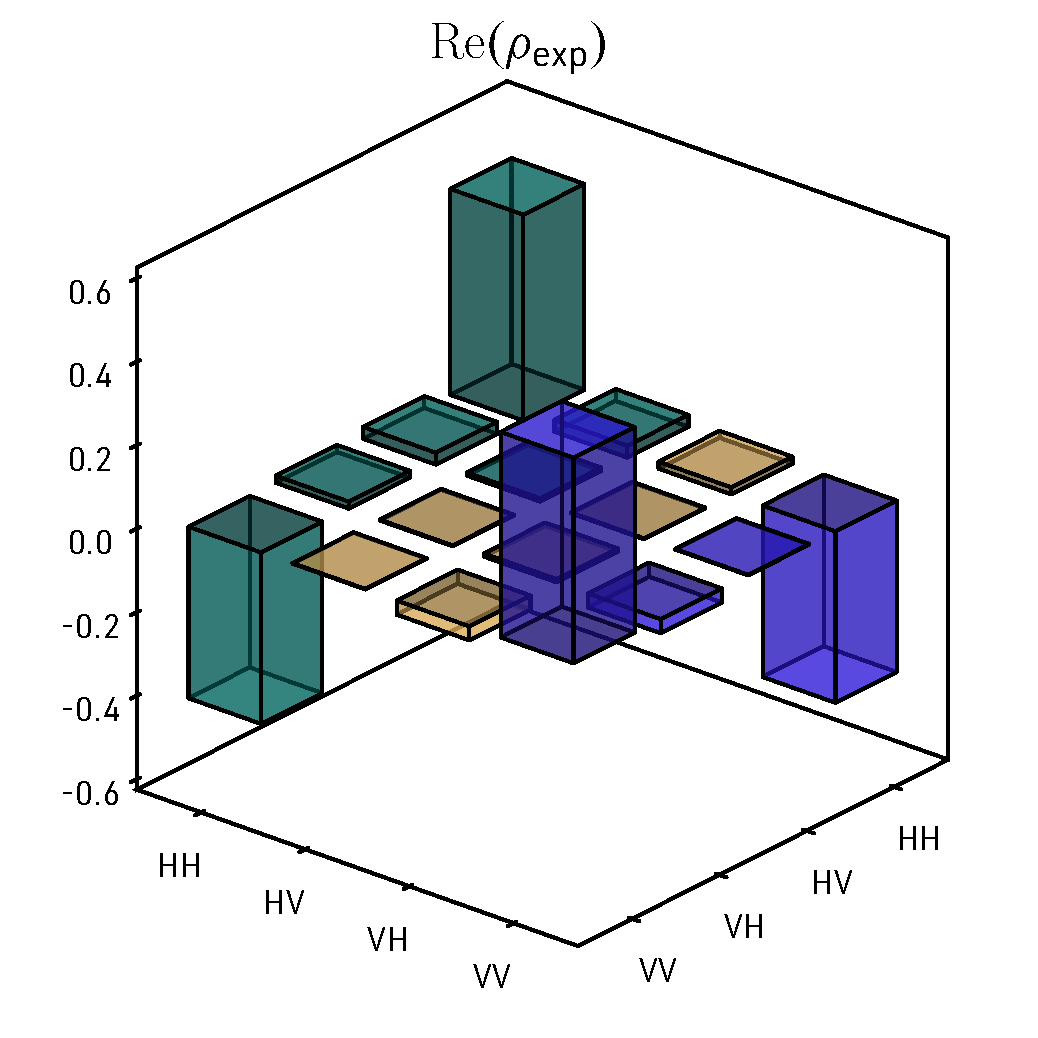
\includegraphics[width=0.5\textwidth]{EPR_den_mat_Re.pdf}
	}
	\subfloat[\labelFigure{epr_den_mat_img}]
	{ %
        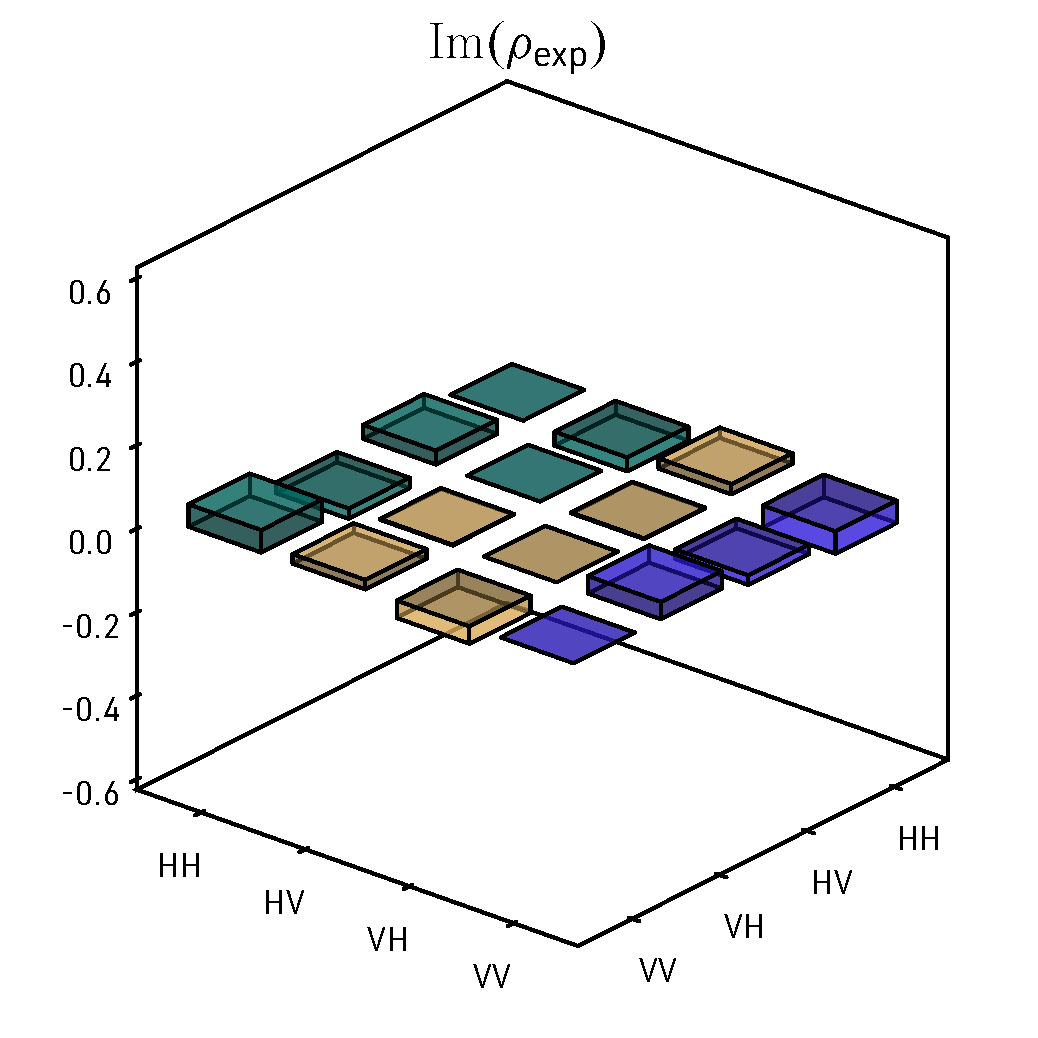
\includegraphics[width=0.5\textwidth]{EPR_den_mat_Im.pdf}
	}
\caption[Density matrix of a state estimated by maximum likelihood tomography from experimental data after optimization.]{Density matrix of a state estimated by maximum likelihood tomography from the experimental data given in~\protect\refTableOnly{tomo_analysis} after optimization. \textbf{(a)} Real part of the estimate of $\varrho$. \textbf{(b)} Imaginary part of the estimate of $\varrho$.}
	\labelFigure{2q_tomo}
\end{figure}

\noindent
Alas, while the above results improve over the preliminary results and are in good agreement with expected state $\ket{H_1,H_2} - \ket{V_1,V_2}$, unwanted artefacts such as the apparent loss in the coherences of the two orthogonal polarizations and a small, non-negligible mixedness of the state, in the reconstructed state still persist. The origins of some of these unwanted artefacts can be attributed to systematic errors, such as those stemming from efficiencies of the various optical components in the experiment\footnote[][-30pt]{PBS transmission and reflection efficiencies, photon detector efficiency and their coupling efficiency to optical fibres, collection efficiencies etc.}. 

\bigskip
\noindent
While the origins of the loss of coherences are often attributable to the many decoherence mechanisms of polarization-entangled sources, which vary from source to source and dependent on nature and application of the experiment at hand. We will briefly outline the two decoherence mechanisms that are relevant to our application, following references~\cite{Akselrod_2007, Akselrod_err_2007, Baek_2008, Rangarajan_2009}.

\clearpage
\noindent
An ideal process of type-I \acs{SPDC} has stringent phase matching conditions; for a pump photon incident on a crystal down converts to two photons, a signal and an idler photon, with the same polarization. The entire process must both conserve momentum and energy, which give rise to the aforementioned conditions:

\begin{align}
	\labelEquation{phase_match}
	\vec{k}_i + \vec{k}_s = \vec{k}_p, \nonumber \\
	\omega_i + \omega_s = \omega_p,
\end{align}

\noindent
where $\vec{k}$ and $\omega$ are the wave vector and frequency of the photon respectively. The subscripts $i$, $s$ and $p$ refer to the idler, signal and pump photon respectively. For a frequency degenerate type-I \acs{SPDC} process, the idler and signal photons have half the frequency of the pump photon individually. In an ideal experiment, one expects the phase-matching conditions to be perfectly satisfied, in an actual experiment this is not the case. In reality, there is often a phase mismatch, which enters into~\refEquationOnly{phase_match} \via an additional effective wave vector $\vec{\Delta}$, which has a non-trivial effect on the spectral properties of the process. 

\begin{align}
	\labelEquation{phase_mismatch}
	\vec{k}_i + \vec{k}_s + \vec{\Delta} = \vec{k}_p.
\end{align}

\noindent
Ideally, for a type-I non-collinear degenerate \acs{SPDC} process, only frequency-degenerate photon pairs are emitted at the emission angle of the light cones. However, due to the phase mismatch, it is possible for the process to also produce non-degenerate frequency photons pairs. The emission angles of the non-degenerate pairs will not always be asymmetric around pump beam; the findings in Ref.~\cite{Baek_2008} report the production of non-degenerate pairs at \SI{662.2}{\nano\meter} (signal photon) and \SI{747.3}{\nano\meter} (idler photon) respectively, with the signal photon within the collection angle of their system (around $3^{\circ}$), while the idler photon falls outside this collection angle, hence does not contributing to the single photon rates. 

\bigskip
\noindent
The said effect produces spectral profiles for both signal and idler photons that are asymmetric around the degenerate frequency. The result of this spectral profile asymmetry along with the geometry of a experiment, have a bearing on the two-photon joint spectra which determines the coincidence counts. Baek and Kim ~\cite{Baek_2008} show that the joint spectra is significantly reduced in comparison to the spectral profile of the signal/idler photon pairs, and limited by the collection angles in their experiment, $2.95^{\circ} - 3.17^{\circ}$; this collection range does not collect one of the photons from a non-degenerate pair.  As a result, the two-photon spectra can also have asymmetric spectral profile around the degenerate frequency, which can be significantly altered by small alignment errors. 


\bigskip
\noindent
A way to compensate for this spectral asymmetry is by way of spectral filtering over the bandwidth of a narrow bandwidth filter around the degenerate frequency, the spectral profiles of the idler and signal photons, and consequently two-photon joint spectra are made more similar to one another, by effectively filtering out the unwanted non-degenerate photon pairs. This method of compensation comes at the expense of collection efficiency of the experiment. The spectral filters in our experiment have quite a broad bandwidth, centred at \SI{800}{\nano\meter} with a \acs{FWHM} of \SI{40}{\nano\meter}, thus it is not far-fetched to suspect the presence of non-degenerate photon pairs, which is by evidenced by the significantly high single count rate in comparison to coincidence rate (by roughly a scale $\sim 0.3$). 

\clearpage
\noindent
We attempted to use narrow bandwidth filters, centred at $\SI{810}{\nano\meter}$ with a \acs{FWHM} of \SI{10}{\nano\meter}, which did not improve the results by much, upon inspection, we found that when filtering a white light source\footnote{Fianium WhiteLase micro with spectrum $<$\SI{450}{nm} to $>$\SI{2000}{nm} with a pulse width of $\approx$\SI{6}{ps} and a repetition rate of \SI{20}{MHz}.} the two filters had non-overlapping regions of considerable size in their spectral profiles. One of the interference filters was not centred at \SI{810}{\nano\meter} (as indicated by the manufacturer) but slightly higher, which for the interim explains why the results did not improve by much.

\bigskip
\noindent
Another dominant decoherence mechanism, particularly for a paired-\acs{BBO} type-I \acs{SPDC} source, is one that degrades the temporal indistinguishability of the down converted photons. Crudely represented, the two crystals having finite thickness, means the two down-conversion processes in the two crystals will occur at slightly different times (order of femtoseconds). Over the thickness of the crystals, both birefringent and dispersive effects influence the group velocities of both signal and idler photons, and subsequently their emission times from the two crystals. If the assumption is that two down-conversion processes take place at halfway the length of each crystal, then time taken by the signal and idler photons to traverse the length $L$ of the two crystals, can be calculated as follows~\cite{Rangarajan_2009}.  For photons down converted in the first crystal:

\begin{itemize}
	\item[\emph{Primo}] A pump photon will traverse half of the length of the first crystal where it is extraordinary polarized, after which it down converts resulting in a polarization perpendicular to the original and hence ordinary polarized. 
	\item[\emph{Secondo}] The resulting signal/idler photon will traverse the second half of the first crystal ordinary polarized.
	\item[\emph{Terzo}] After exiting the first crystal, the signal/idler photon will traverse the full length of the second crystal extraordinary polarized.
\end{itemize}

\noindent
The time spent by a signal photon in each of the three stages above depends on the refractive-index-dependent group velocities of ordinary and extraordinary photons in the two crystals and the length $L$:

\begin{align}
	t_s &= \frac{L}{2V^{e}_g(\omega_p)} + \frac{L}{2V^{o}_g(\omega_s)} +
	\frac{L}{V^{e}(\omega_s)},
\end{align}

\noindent
the reasoning is similar for photons down converted in the second crystal, and gives: 

\begin{align}
	t'_s &= \frac{L}{V^{o}_g(\omega_p)} + \frac{L}{2V^{e}_g(\omega_p)} + \frac{L}{2V^{o}_g(\omega_s)},
\end{align}

and the net delay $\Delta t_s$ between the two down conversion processes is given by

\begin{align}
	\Delta t_s  = t'_s - t_s = L \left(\frac{1}{V^{o}_g(\omega_p)} - \frac{1}{V^{e}_g(\omega_s)} \right).
\end{align}

\noindent
The above time difference leads to the degradation of the temporal indistinguishability between the two light cones; photons belonging to one light cone will be delayed by $\Delta t_{s/i}$ relative to the photons from the other light cone. 

\clearpage
\noindent
Rangarajan~\etal~\cite{Rangarajan_2009} derive an expression for the density matrix of the two-photon down converted state with such a delay:

\begin{align}
	\varrho'  = \frac{1}{2} \mqty(
		1 & 0 & 0 & \nu(\Delta t_s, \Delta t_i) \\
		0 & 0 & 0 & 0 \\
		0 & 0 & 0 & 0 \\
		\nu^*(\Delta t_s, \Delta t_i) & 0 & 0 & 1
	),
\end{align}

\noindent
where $\nu(\Delta_s, \Delta_i)$ is dependent on the two-photon joint spectra. As expected, we note that this decoherence mechanism has no effect on the two populations but only affects the coherence between the two polarizations. Refs.~\cite{Akselrod_2007, Akselrod_err_2007, Rangarajan_2009} recommended the use of birefringent crystals, with the same but opposite time delay between extraordinary and ordinary components of the pump photons, to pre(post)compensate for the delay between the emission-times of the two down conversion processes. With use of such techniques, they were able to state fidelities in excess of $0.977$.

\section{Concluding remarks}
\labelSection{C4_concluding_remarks}
In this chapter, we described and conducted an experiment based on \acs{SPDC}, generating a two-photon two-qubit polarization-entangled state. The generated state is fully characterized through \acs{QST}, recovering its density matrix, from which other physical quantities of interest, such as those quantifying the degree of entanglement possessed by the state can be derived from. The \acs{SPDC} source is optimized, with a rule of thumb procedure described in the text, to generate one of the Bell states ($\ket{\Phi^{-}}$). We repeat this process until we achieve a fidelity of $0.90$. In comparison to similar demonstrations in the current literature, which can achieve fidelities in access of $0.97$, this is a relatively is low fidelity, nevertheless the obtained result is satisfactory to our experimental needs. Lastly, we briefly outlined a description of the two decoherence mechanisms for paired \acs{BBO} type-I non-collinear \acs{SPDC} and how these maybe counteracted to improve the fidelity of the generated polarization-entangled state. In the chapter that follows, we will describe how the polarization-entangled state generated by this Bell-state photon pair source may be extended to accommodate an additional qubit through a different \acs{DOF}.

\chapter{Path-polarization-entangled photons}
\labelChapter{path_polarization_entangled_photons}

\begin{epigram}{\textit{Peter Shor, Quantum Poetry Tweet Collection}}
	\enquote{
		Am I a wave? Am I a particle? Am I analog or digital?\newline
		The answer surely must be both or none.\newline
		My laws say quarks and clocks alike show interference,\newline
		That if you watch a state, it never changes,\newline
		That two entangled systems act as one.} 
\end{epigram}

\section{Introduction: Multi-degree of freedom entanglement}
\lettrine[lines=3]{T}{he} preceding chapter describes the generation of a two-photon two-qubit polarization-entangled state \via the process of \acs{SPDC} with type-I phase matching. In this chapter, we endeavor to describe and experimentally realize one possible way to enlarge this two-qubit state to a state of more qubits. From the previous chapter, one can at least get an inkling that the generation of entangled photons by way of \acs{SPDC} is appealing due to its accessibility, in the case of type-I \acs{SPDC}, ease of alignment and relatively high photon counts in comparison to type-II phase matched \acs{SPDC}~\cite{Kwiat_1999}. Thus one could possibly conceive of a way to enlarge the aforesaid two-qubit state \via the same \acs{SPDC} process; a string of successive \acs{SPDC} processes producing a pair of entangled photons at each step, as done in the experiments of Ref.~\cite{Lu_2006,Huang_2011,Wang_2016}. One potential and sizeable obstacle to such methods is decoherence. As briefly alluded to in the previous chapter, unless one incorporates methods to counteract some of the effects of decoherence on \acs{SPDC} sources such as phase-compensation ~\cite{Akselrod_2007,Rangarajan_2009} to improve the brightness of the source, experiments making use of cascaded \acs{SPDC} processes typically suffer from low efficiencies~\footnote{Due to the decoherence mechanisms of \acs{SPDC} source, but also due to inefficiencies of the optics in the experiment, \eg the collection and detection inefficiencies.}

\bigskip
\noindent
Hitherto, we have only considered the polarization \acs{DOF}, however photon pairs generated in this way also possess various forms of entanglement. The phase-matching conditions for \acs{SPDC} give rise to conservation laws for both energy and momenta of the photon pairs, as a result the pairs are entangled in these continuous \acs{DOFS} as well. The experiments of Rarity \etal~\cite{Rarity_1990} and Kwiat \etal~\cite{Kwiat_1993} were few of the first to demonstrate a violation of a Bell-inequality for a continuous \acs{DOFS}, energy (and time) and momentum, respectively. 


\clearpage
\noindent
Relatively recent experiments have given evidence that, the process of \acs{SPDC} conserves the orbital angular momentum~\cite{Mair_2001,Vaziri_2002}; demonstrating the generation and analysis of coherent superposition of \gls{LG} transverse spatial modes, and a violation of a Bell-inequality for qutrits. A theoretical justification for this conservation law was later derived by Franke-Arnold \etal~\cite{Franke-Arnold_2002} from the phase-matching conditions of \acs{SPDC}. For a \acs{LG} mode pump beam carrying the quantum number $l_\text{pump}$~\footnote{Every photon in the beam carries an orbital angular momentum of $\hbar l_\text{pump}$~\cite{Allen_1992}.}, the sum of the corresponding quantum number for signal and idler photons must be the same, \ie $l_\text{signal} + l_\text{idler} = l_\text{pump}$. For a pump beam with $l_\text{pump}=0$, the resultant two-photon \gls{OAM} state will be

\begin{align}
	\ket{\psi}_\text{OAM} &= \alpha_{0,0}\ket{0_1,0_2} + \alpha_{1,-1}\ket{1_1,-1_2} + \alpha_{-1, 1}\ket{-1_1, 1_2} + \ldots\ldots,
\end{align}

\noindent
with the \acs{LG} modes spanning a countably-infinite dimensional Hilbert space, where the kets denote \acs{OAM} states labelled with the indices $l$ and $\alpha$'s denoting their corresponding probability amplitudes; the subscripts $1$ and $2$ represent the signal and idler photons, respectively. 

\bigskip
\noindent
Photons produced \via \acs{SPDC} could result in photons possessing non-classical correlations in degrees of freedom simultaneously, with each \acs{DOF} independently addressable for such measurements. Such multiply-entangled states are called \enquote{hyper-entangled} states, coined by Kwiat~\cite{Kwiat_1997}. For instance, photon pairs produced by a paired \acs{BBO} type-I \acs{SPDC} process, generate a state represented by the product state:

\begin{align}
	\labelEquation{hyper_ent}
			\ket{\Psi}	&\sim (\ket{H_1,H_2} - \ket{V_1,V_2}) \otimes (\ket{-1_1,-1_2} + \ket{1_1,1_2}).
\end{align}

\noindent
For this particular state, each \acs{DOF} is independently addressable and in a well defined state, that is, measurements of observables on either subsystem, whether of polarization or orbital angular momentum, have no bearing on the other subsystem. Formally, a partial trace over the subsystem in either \acs{DOF} leaves the other subsystem unaffected.

\begin{align}
 	\Tr_A(\varrho_{AB}) &= \Tr_A(\varrho_A \otimes \varrho_B), \nonumber \\
 						&= \displaystyle\sum_{i=0}^{3}\ev{\varrho_A}{i}\otimes\varrho_B,\nonumber \\
 						&= \mathds{1}_A \otimes \varrho_B, \nonumber \\
 						&= \varrho_B,
 \end{align}

\noindent
where $\varrho_A = 1/2(\ket{H_1,H_2} - \ket{V_1,V_2})(\bra{H_1,H_2} - \bra{V_1,V_2})$ and $\varrho_B = 1/2(\ket{-1_1,-1_2} + \ket{1_1,1_2})(\bra{-1_1,-1_2} + \bra{1_1,1_2})$, and where $\ket{i}$'s are from the orthonormal basis set $\{\ket{H_1,H_2}, \ket{H_1,V_2}, \ket{V_1,H_2}, \ket{V_1,V_2}\}$ for the polarization subsystem. It is also possible for a \acs{SPDC} source to generate a state of the kind:

\begin{align}
	\labelEquation{hypo_ent}
	\ket{\Psi} \sim (\ket{H_1,H_2,-1_1,-1_2} + \ket{V_1,V_2,1_1,1_2}).
\end{align}

\clearpage
\noindent
Such a state is a little different from the state of~\refEquationOnly
{hyper_ent}. The first obvious difference is this state isn't a product state; the state in either \acs{DOF} can no longer be described separately, we can only collectively describe it by referencing to the state of the other \acs{DOF} \ie the full joint state is non-separable. For such a state (as we've seen elsewhere), a measurement in one \acs{DOF} has a bearing on the other \acs{DOF}. For instance, taking the partial trace over the \acs{OAM}\acs{DOF} yields:

\begin{align}
	\Tr_{CD}(\varrho_{ABCD}) &= \Tr_{AB}(\ket{H_1,H_2,-1_1,-1_2}\bra{H_1,H_2,-1_1,-1_2} \nonumber \\
						&+ \ket{H_1,H_2,-1_1,-1_2}\bra{V_1,V_2,1_1,1_2} \nonumber \\
						&+ \ket{V_1,V_2,1_1,1_2}\bra{V_1,V_2,1_1,1_2}  \nonumber \\
						&+ \ket{V_1,V_2,1_1,1_2}\bra{H_1,H_2,-1_1,-1_2}) \nonumber \\
						&= \ket{H_1,H_2}\bra{H_1,H_2} + \ket{V_1,V_2}\bra{V_1,V_2}.
\end{align}

\noindent
where the partial trace is performed over the basis set $\{\ket{-1_1,-1_2}, \ket{-1_1,1_2}$ $, \ket{1_1,-1_2}, \ket{-1_1,-1_2}\}$. Note that the resultant state is one in which coherences between $\ket{HH}$ and $\ket{VV}$ are completely destroyed; the density matrix of the state has no off-diagonal elements. The said states are called \enquote{hypoentangled states}~\cite{Nathan_PhD}, their defining feature is that they exhibit simultaneous entanglement, but when one of \acs{DOFS} is considered independently, the entanglement in that \acs{DOF} isn't preserved. 

\begin{marginfigure}
	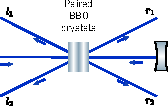
\includegraphics[width=\textwidth]{BF_SPDC.pdf}
	\caption[A \acs{SPDC} source with two concatenated \acs{BBO} crystals stimulated by a pump beam in both directions.]{A \acs{SPDC} source with two concatenated \acs{BBO} crystals stimulated by a pump beam in both directions. The two pairs are emitted in different directions, $l_1, l_2$ and $r_1, r_2$ denoting the four spatial modes.}
	\labelFigure{bf_spdc}
\end{marginfigure}

\bigskip
\noindent
The first demonstration and complete characterization of a hyper entangled photonic quantum system was done by Langford~\cite{Nathan_PhD}, generating and completely characterizing a $144$-dimensional state, simultaneously and independently entangled in polarization, transverse (\acs{OAM}) spatial modes and photon emission times (time-bin encoding). The rarity and novelty of such a demonstration would seem to suggest the experimental difficulity/novelity of realizing photonic states of this kind. Indeed, exerting control over different \acs{DOFS} is not trivial. They often necessitated sophisticated and tricky mode (spatial and/or temporal) matching requirements to implement in practice.

\bigskip
\noindent
The same partly holds true in practice, for similar experiments that generate hyper(hypo) entangled photonics states through polarization and momentum (directions of the emitted photons) \acs{DOFS}. Here, a pump beam stimulates a \acs{SPDC} crystal in both directions resulting in polarization-entangled photon pairs in both directions, which are then appropriately isolated to four optical path modes ($l_1, l_2\text{ and }r_1, r_2$ in~\refFigureOnly{bf_spdc}). If the paired path modes, one mode from the backward photon pair and another from the forward photon pair ($l_1\text{ and }r_1$ and $l_2\text{ and }r_2$) are overlapped temporally (and spatially) on the input ports of a 50:50 beam splitter (see~\refFigureOnly{temporal_delay}), can they can realize a hyperentangled state of the form~\cite{Yang_2005}:

\begin{align}
	\ket{\Psi} \sim (\ket{H_1,V_2} \pm \ket{H_1,V_2})\otimes(\ket{r_2,l_2} \pm \ket{l_1,r_1}),
\end{align}

\begin{marginfigure}
	\raggedright
	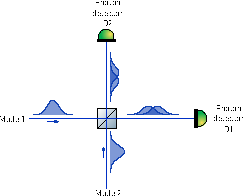
\includegraphics[width=\textwidth]{temporal_delay.pdf}
	\caption[Temporal delay between two spatial modes incident on the input ports of a 50:50 beam splitter.]{Temporal delay between two spatial modes incident on the input ports of a 50:50 beam splitter. The temporal delay leads to temporal indistinguishability, which in an interferometric experiment has a debilitating effect on the observed interference.}
	\labelFigure{temporal_delay}
\end{marginfigure}


\noindent
alternatively if paired path modes belong to the same photon pair ($l_1\text{ and }l_2$ and $r_1\text{ and }r_2$) are similarly overlapped temporally (and spatially) generate the hypoentangled state~\cite{Chen_2007}:

\begin{align}
	\ket{\Psi} \sim (\ket{H_1, H_1} + \ket{V_1,V_2})\ket{l_1,l_2} + (\ket{H_1, H_2} - \ket{V_1,V_2})\ket{r_1,r_2}).
\end{align}


\noindent
In this kind of experimental setup, in addition to the spatial and/or temporal mode matching requirements, the generated state depends on the rate of photon pair emissions in both directions.


\clearpage
\noindent
For the states described above, the aforesaid rates should be equalized. It is known for a \acs{SPDC} source, particularly non-collinear non-degenerate \acs{SPDC}, the resultant (single and joint) spectral profiles, hence the two-photon emission rates and output spatial modes, are dependent on the focus of the pump beam~\cite{Carrasco_2006}. Hence, the experiments in Refs.\cite{Yang_2005, Chen_2007} equalize the emission rates of the two \acs{SPDC} processes (backwards and forwards) using an appropriate arrangement of focusing optics (\ie lens). These added complications compel us to consider an experimental scheme for enlarging our two-photon state from the previous chapter that explicitly avoids them. We consider adopt the experimental scheme of Park \etal~\cite{Park_2007}, which uses a single-photon pair source to realize a polarization-path-entangled state. Hence we describe the experimental design next.

\section{Experimental design}
In this experiment, we extend the experimental setup from the previous chapter to accommodate an additional path qubit. The experimental setup is shown in~\refFigureOnly{experiment_2}; conceptually, this experiment is again simple to describe. The experimental design is similar to the design in the previous chapter (see~\refFigureOnly{experiment_1}) with only one minor addition; in one of the arms, arm $1$ in the figure, the photon beam is incident on a \acs{PBS}, transmitting horizontally-polarized photons and reflecting vertically-polarized photons, which effectively defines our path modes ($l_1\text{ and }r_1$). Our \acs{SPDC} source produces a state close to $(\ket{H_1,H_2} - \ket{V_1,V_2})/\sqrt{2}$, at the dashed line after the action of the \acs{PBS} as shown in~\refFigureOnly{experiment_2} this state becomes:

\begin{align}
	\labelEquation{after_pbs}
	\ket{\Psi_1} = \frac{\ket{H_1, r_1, H_2} - \ket{V_1, l_1, V_2}}{\sqrt{2}}.
\end{align}

\noindent
We designate the polarization and path states of the photon in arm $1$ as qubit $1$ and qubit $2$, respectively and the polarization of the photon in arm $2$ as qubit $3$. Furthermore, relabelling $\ket{H}(\ket{V})$ as $\ket{0}(\ket{1})$, and similarly $\ket{r}(\ket{l})$. The state in~\refEquationOnly{after_pbs} becomes

\begin{align}
	\labelEquation{standard_ghz}
	\ket{\Psi'_1} = \frac{\ket{0, 0, 0} - \ket{1, 1, 1}}{\sqrt{2}} = \frac{\ket{0}^{\otimes 3} - \ket{1}^{\otimes 3}}{\sqrt{2}}.
\end{align}

\noindent
The state in~\refEquationOnly{standard_ghz} is locally equivalent to \acs{GHZ} state~\footnote[][100pt]{Applying the unitary operator ($\mathds{1}_1Z_2\mathds{1}_3$) to $\ket{\Psi}$, we recover the \acs{GHZ} state in its standard form $(\ket{0}^{\otimes 3} + \ket{1}^{\otimes 3})/\sqrt{2}$.}. Similarly, if we apply the unitary operator $U=\mathds{1}Z_2\mathds{1}_3$ to state in~\refEquationOnly{standard_ghz} and proceed to rotate the coordinate system for all our polarization measurements by $\theta=-22.5^{\circ}$ ($\ket{H} \mapsto (\ket{H}+\ket{V})/2, \ket{V} \mapsto (\ket{H} - \ket{V})/\sqrt{2}$), $\ket{\Psi_1}$ becomes:

\begin{align}
	\ket{\Psi_1} = \frac{\ket{+, 0, +} - \ket{-, 1, -}}{\sqrt{2}},
\end{align}

\noindent
where $(\ket{\pm} = \ket{0}\pm\ket{1})/\sqrt{2}$. The above state is a three-qubit linear graph state, which may be generated by applying controlled-$Z$ operations on neighboring qubits ($1-2$ and $2-3$) of the initial resource state $\ket{+}_1\ket{+}_2\ket{+}_3$.

\bigskip
\noindent
The rest of the optics in arm $1$ of the experimental setup are designated for measurement and analysis, consisting of a \acs{MZI}, which combines the two path modes on the output ports of a 50:50 beam splitter. 

\clearpage
\begin{figure*}[t!]
  \centering
  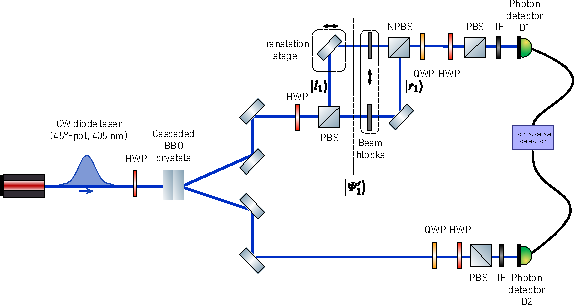
\includegraphics[width=1.0\textwidth]{experiment_2.pdf}%
	\caption[Experimental setup for generation and measurement of a two-photon three-qubit path-polarization-entangled state locally equivalent to a \acs{GHZ} state.]{Experimental setup for generation and measurement of a two-photon three-qubit path-polarization-entangled state locally equivalent to a \acs{GHZ} state.  \gls{HWP}, \gls{QWP}, \gls{BBO}, \gls{PBS}, \gls{NPBS}, translatable mirror,  translatable beam blocks, and \gls{IF}. A photon pair is created whenever a laser pump photon with \SI{405}{nm} wavelength is incident on the paired \acs{BBO} crystals cut for type-I \acs{SPDC}, generating photons at \SI{810}{nm}. One of the photons enters a \acs{MZI} where path modes are made to interfer when combined on , at the dashed line the joint state $\ket{\Psi'_1}$ is locally equivalent to a \acs{GHZ} state. Each photon is guided by a set of mirrors to a \acs{QWP}, \acs{HWP}, and \acs{PBS} which are used to perform polarization measurements of the quantum state. Finally, each photon is sent to an \acs{IF} at \SI{800}{nm} with a bandwidth of \SI{40}{nm} and collected by a \gls{SMF} and sent to a photon detector. Each photon detector produces an electronic signal and sends it to the coincidence counting electronics, which count the signals that arrive simultaneously.}
  \labelFigure{experiment_2}
\end{figure*}


\noindent
One of the path modes is reflected off a mirror on an motorized translation stage (MTS25/M-Z8 - 25 mm (0.98") Motorized Translation Stage with a KDC101 K-Cube Motor Controller), which can used to change the relative phase difference between the two path modes, projecting the path qubit to states on the$x$-$y$ plane of the Bloch sphere (on the equator) with the form:

\begin{align}
	\ket{\varphi} = \frac{\ket{0} + e^{i\varphi}\ket{1}}{\sqrt{2}}.
	\labelEquation{equator_eq}
\end{align}

\noindent
In both paths, there are beam blocks mounted on an electronically-controlled translation stage, which can either block one of the paths or let them both pass. Whenever we block one of the paths, we project out one of the states $(\ket{0}, \ket{1})$ depending on which path is blocked. The combined beam on one of the output ports of the beam splitter is sent to polarization analysis optics and eventually to the photo detector, consisting of a rotatable \acs{QWP} and \acs{HWP}, a \acs{PBS} and an \acs{IF} at \SI{800}{nm} with a \SI{40}{nm} bandwidth. After this stage, the beam goes to a photon detector \via a fibre launch coupled to the detector with a \acs{SMF}. The optical path of arm $1$ is slightly longer than that of arm $2$, for this reason we modify our coincidence counting electronics to add a variable delay to arm $2$ to roughly compensate for the delay on arm $1$ introduced by the \acs{MZI}. Through a bit of tinkering, we find that a delay between \SI{0.5}{ns} to \SI{1.5}{ns} works well enough; our delay electronics operate in increments of \SI{0.5}{ns}, the true delay is probably somewhere in between this range.

\bigskip
\noindent
To match the optical path difference of the two paths to be on the order of the coherence length of the down-conversion photons ($\simeq$ \SI{60}{\micro\meter}) we used a broad spectrum white laser source. The beam from this laser source is guided into the experiment through fibre coupler we previously used to hold the \acs{SMF} taking the beams to the detectors. It is then sent through the \acs{MZI} and collected by another fibre coupler near the crystals coupled with a \acs{SMF} into a spectrometer (Thorlabs CCS200/M with a wavelength range of \SI{200}{nm}-\SI{1000}{nm}). 


\clearpage
\noindent
We can thus resolve the interference fringes in spectra near our collection bandwidth (\SI{800}{nm}$\pm$\SI{40}{nm}) by translating the mirror inside the \acs{MZI} to obtain optimal matching of the path lengths of two arms of the \acs{MZI}. Once the \acs{MZI} is optimized for the coherence length of the down-converted photons, when the two path modes from one of the down-conversion photons combine on the output ports of the 50:50 beam splitter, the state $\ket{\Psi_1}$ of~\refEquationOnly{after_pbs} then becomes:

\begin{align}
	\ket{\Psi_2} = \frac{1}{2}(e^{\varphi_{1}}(\ket{H_1, p_1, H_2} + \ket{H_1, q_1, H_2}) \nonumber \\
	-e^{\varphi_{2}}(\ket{V_1, p_1, V_2} - \ket{V_1, q_1, V_2})),
\end{align}

\noindent
where $p_1, q_2$ are the path modes of the output ports of the beam splitter and $\varphi_{1}, \varphi_{2}$ are the phases acquired by path modes ($l_1$ and $r_1$) by the time they are incident on the beam splitter. Here we adopt the convention $\ket{r_1} \mapsto (\ket{p_1}-\ket{q_1})/\sqrt{2} \text{ and } \ket{l_1} \mapsto (\ket{p_1}+\ket{q_1})/\sqrt{2}$ for the 50:50 beam splitter. After a bit of algebraic deadlifting, the preceding equation becomes:

\begin{align}
	\ket{\Psi_2} = \frac{1}{2}(\ket{p_1}(\ket{H_1, H_2} - e^{i(\varphi_2 - \varphi_1)}\ket{V_1, V_2})) + \nonumber \\
	\ket{q_1}(\ket{H_1, H_2} + e^{i(\varphi_2 - \varphi_1)}\ket{V_1, V_2}))).
\end{align}

\noindent
The mode $q_1$ goes through the polarization analysis optics and eventually to the photon detector yielding:

\begin{align}
	\labelEquation{psi_meas}
	\ket{\Psi_2} = \frac{1}{\sqrt{2}}(\ket{H_1, H_2} + e^{i\varphi}\ket{V_1, V_2}),
\end{align}

\noindent
where $\varphi = \varphi_2 - \varphi_1$. Note that the phase difference between the two path modes influences the state measured by the polarization analysis optics. We can thus infer this phase difference with a similar procedure from our observations in~\refEquationOnly{obs_1} and~\refEquationOnly{obs_2} to optimize the \acs{SPDC} source for a particular Bell state. By inserting a \acs{HWP} in the path mode $r_1$, and setting it at $\theta=45^{\circ}$ ($\ket{H} \leftrightarrow \ket{V}$), ~\refEquationOnly{psi_meas} becomes:

\begin{align}
	\labelEquation{psi_cal}
	\ket{\Psi_2'} &= \frac{1}{\sqrt{2}}(\ket{H_1, H_2} + e^{i\varphi}\ket{H_1, V_2}), \nonumber \\
				  &= \frac{1}{\sqrt{2}}\ket{H_1}(\ket{H_2} + e^{i\varphi}\ket{V_2}).
\end{align}

\noindent
We infer the value $\varphi$ by choosing the appropriate projectors, for instance projecting $P_{HR} = \op{H_1}\otimes\op{L_2}$ on the above state and a bit algebraic deadlifting one obtains the expression for detection probability:

\begin{align}
	&\ev{P_{HR}}{\Psi_2'} = \frac{1}{2} - \frac{1}{2}\sin{\varphi}.
\end{align}

\noindent
Thus moving the translation stage mounted with the mirror, we can minimize the observed coincidence counts which would then correspond to $\varphi = \pi/2$, and maximized coincidence counts correspond to the setting $\varphi = - \pi/2$. The aforementioned values of $\varphi$ project the path qubit in~\refEquationOnly{equator_eq} to $(\ket{0}+i\ket{1})/\sqrt{2}$ and $(\ket{0}-i\ket{1})/\sqrt{2}$, which are the positive and negative eigenvectors of the Pauli matrix $Y$. Any value of $\varphi$ maybe inferred similarly. 


\clearpage
\noindent
Therefore, any equatorial basis measurement of the form:

\begin{align}
	\mathcal{B}(\varphi) = \left\{\frac{\ket{0} + e^{i\varphi}\ket{1}}{\sqrt{2}}, \frac{\ket{0} - e^{i\varphi}\ket{1}}{\sqrt{2}} \right\},
\end{align}

\noindent
can be performed on the path qubit. Together with the $Z$ basis measurements ($\{\ket{0}, \ket{1}\}$), it is possible to perform measurements, measuring each of the eigenvectors of Pauli matrices; which allows us to independently address each of the three qubits for control and measurements of quantum-mechanical correlations of the generated state.

\section{Results}

To get an inkling of how well the \acs{MZI} can contrast between constructive and destructive interference of the two path modes, we measure the fringe visibility for down-conversion photons in following configurations: (i) When only one of the \acs{BBO} crystals, producing the $H$-polarized light cone is stimulated. (ii) When only one of the \acs{BBO} crystals, producing the $V$-polarized light cone. (iii) When both \acs{BBO} crystals are stimulated. For all three configurations, there is a \acs{HWP} at the gate of the interferometer (before the PBS) set to $22.5^{\circ}$ ($\ket{H} \leftrightarrow \ket{D}$), and the half wave-plate in the path mode $r_1$ is set to $\theta=45^{\circ}$, giving the state in~\refEquationOnly{psi_cal} and project out $P_{HD} = \op{H_1}\otimes\op{D_2}$, giving the expression for the detection probability 

\begin{align}
	&\ev{P_{HD}}{\Psi_2'} = \frac{1}{2} + \frac{1}{2}\cos{\varphi},
\end{align}

\noindent
by translating the mirror in the \acs{MZI} in increments of \SI{40}{nm}, we can vary $\varphi$. Typical (normalized) coincidence counts when $\varphi$ is varied for the three aforesaid settings are shown in~\refSubfigureOnly{hh_fringes}, ~\refSubfigureOnly{vv_fringes} and~\refSubfigureOnly{epr_fringes} of ~\refFigureOnly{fringes}, respectively\footnote{The fitting function used for the plots is of the form $a \cos{(b x + c) + d}$. The parameters $a,b,c,d$ were found using Mathematica's \texttt{NonlinearModelFit} function.}. It was worth mentioning that the motor translating the stage can resolve translations down to $\sim$\SI{30}{nm}, however this may come at the price of accuracy. In a sporadic fashion, the motor sometimes translates the mirror slightly less or slightly more than the set step size, hence the plots in the figure above show a few slightly sparse regions. We observe close-to-unity fringe visibilities (calculated from the minima and maxima of the fit) of $0.940$, $0.901$ and $0.921$, respectively. The non-ideal spatial overlap between the two path modes and less-than-unity fidelity of the Bell state prior to the \acs{MZI} may explain the less-than-unity fringe visibility. However, we deem these values sufficient and as indicative that the two path modes are indeed interfering with one another and their optical path difference is within the coherence length of the down-conversion photons. 

\bigskip
\noindent
As we have seen elsewhere, to fully characterize an experimentally generated state, one often needs to perform full \acs{QST}; reconstructing an estimate of the density matrix from which physical quantities of interest may be derived. \acs{QST} for a general three-qubit state would require at least $64$ coincidence measurements. However, if we are only interested in the fidelity of the experimentally generated state and detecting whether the said state possesses genuine multi-particle entanglement around the ideal state we expect to observe, it is possible to circumscribe performing a full tomographic analysis to derive the said quantities, at the cost of generality. 


\clearpage

\begin{figure*}[t!]
    \centering
	\subfloat[\labelFigure{hh_fringes}]
	{
        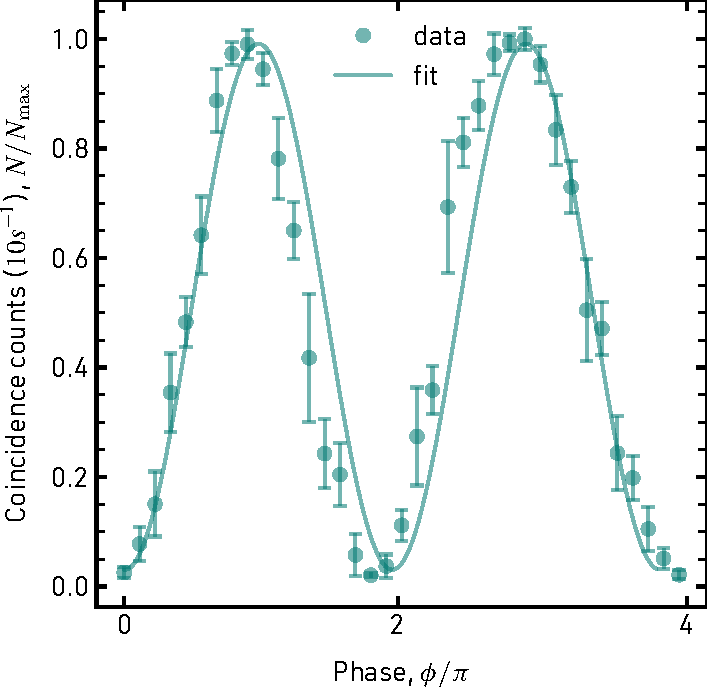
\includegraphics[width=0.33\linewidth]{HH_fringes.pdf}
	}
	\subfloat[\labelFigure{vv_fringes}]
	{
        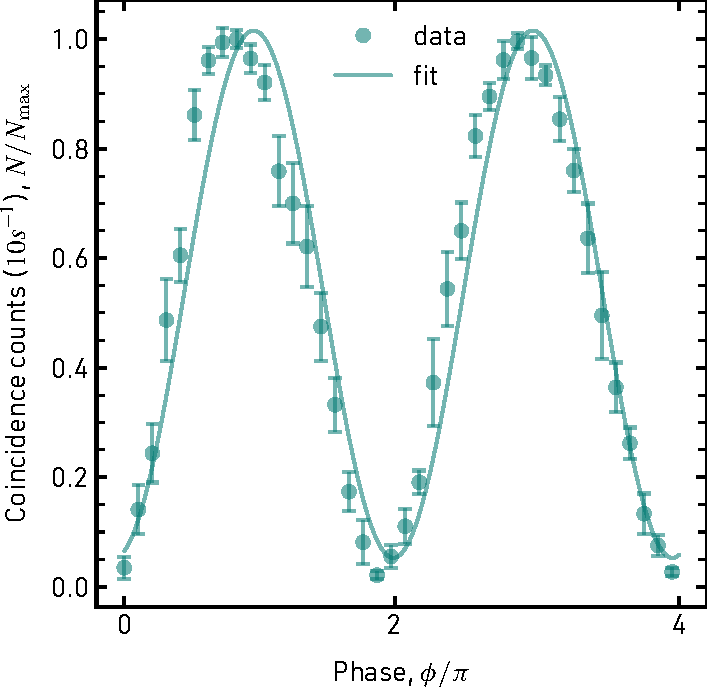
\includegraphics[width=0.33\linewidth]{VV_fringes.pdf}
	}
	\subfloat[\labelFigure{epr_fringes}]
	{
        \includegraphics[width=0.33\linewidth]{EPR_fringes.pdf}
	}
	\caption[Photon coincidence counts traversing the \acs{MZI} as a function of the relative phase between the two paths][6pt]{Photon coincidence counts traversing the \acs{MZI} as a function of the relative phase between the two paths in the interferometer: \textbf{(a)} coincidence counts vs. $\phi$ for pairs of only vertically polarized photons \textbf{(b)} Coincidence counts vs $\phi$ for pairs of only horizontally polarized photons \textbf{(c)} Coincidences counts vs $\phi$ for pairs of entangled photons (Bell state). The error bars represent $95\%$ confidence intervals around the mean value (see section~\protect\refSectionOnly{error_bars} of technical~\protect\refAppendixOnly{appendix_A}.}
	\labelFigure{fringes}
\end{figure*}

\noindent
Without directly deriving the density matrix of the experimentally generated state, we can derive an estimate of the fidelity of the generated state from a reduced set of Pauli operator expectation value measurements, in comparison to full \acs{QST}.  Recall that the fidelity between a expected $\varrho$ and measure state $\varsigma$ is given by~\cite{Mike&Ike}:


\begin{align}
	\labelEquation{tr_fid}
	F(\varrho, \varsigma) = \Tr(\sqrt{\sqrt{\varrho}\varsigma\sqrt{\varrho}}^2) = \Tr(\varrho\varsigma).
\end{align}

\noindent
The desired state $\rho$ may be decomposed into a linear combination of $N$-fold products of $\mathds{1}, X, Y, Z$. In the case of a three-qubit \acs{GHZ} state in its standard form, this decomposition is given by:

\begin{align}
	\labelEquation{decomp}
	\varrho &= \frac{1}{8}(\mathds{1}_1\mathds{1}_2\mathds{1}_3 + \mathds{1}_1Z_2Z_3 + X_1X_2X_3 - X_1Y_2Y_3  \nonumber \\
			&\quad- Y_1X_2Y_3 - Y_1Y_2X_3 + Z_1\mathds{1}_2Z_3 + Z_1Z_2\mathds{1}_3).
\end{align}

\noindent
Estimating of the fidelity of our measured state $\varsigma$ amounts to the evaluation of the expectation values\footnote{For any self-adjoint operator $O$, the expectation value of $O$ with respect to the general state $\varsigma$ is given by, $\expval{O} \equiv \Tr(O\varsigma)$} of above operators with respect to the measured state, and summing them up appropriately.  We reduce the number of unique measurements by noting that the expectation value of the terms $\mathds{1}_1Z_2Z_3, Z_1\mathds{1}_2Z_3 \text{ and } Z_1Z_2\mathds{1}_3$ may be derived from the measurement of $Z_1Z_2Z_3$ as their distributions are marginal distributions of $Z_1Z_2Z_3$ when the outcome of the qubit acted on by the identity is not taken into consideration. Similarly, the expectation value of  $\mathds{1}_1\mathds{1}_2\mathds{1}_3$ may derived from any of terms \via marginalization, it is equal to unity in any case\footnote{$\Tr(\mathds{1}_1\mathds{1}_2\mathds{1}_3 \varsigma) = \Tr(\varsigma) = 1$ (normalization condition)}. Thus, we need only evaluate $5$ unique measurements: $X_1X_2X_3, X_1Y_2Y_3,$ $Y_1X_2Y_3,Y_1Y_2X_3, Z_1Z_2Z_3$. Panels~\refSubfigureOnly{xxx},~\refSubfigureOnly{xyy},~\refSubfigureOnly{yxy},~\refSubfigureOnly{yyx} and ~\refSubfigureOnly{zzz} in \refFigureOnly{expvals} show the measurement outcomes ($8$ each) required for the evaluation of the expectation values of the Pauli operators $X_1X_2X_3, X_1Y_2Y_3,$ $Y_1X_2Y_3,Y_1Y_2X_3 \text{ and } Z_1Z_2Z_3$, respectively.  The error bars represent $95\%$ confidence intervals around the mean value (see section ~\refSectionOnly{error_bars} of the technical~\refAppendixOnly{appendix_A}). ~\refTableOnly{expvals} shows the measured expectation values from the measurements in~\refFigureOnly{expvals} of each operator. Evaluating the fidelity using~\refEquationOnly{tr_fid}, and the Pauli decomposition of our expected state in  ~\refEquationOnly{standard_ghz}, we obtain a fidelity of $F_{\varrho}=  0.868\pm0.00996$.

\clearpage

\begin{figure*}[t!]
	\subfloat[\labelFigure{xxx}]
	{
        \includegraphics[width=0.33\textwidth]{XXX.pdf}
	}
	\subfloat[\labelFigure{xyy}]
	{
        \includegraphics[width=0.33\textwidth]{XYY.pdf}
	}
	\subfloat[\labelFigure{yxy}]
	{
        \includegraphics[width=0.33\textwidth]{YXY.pdf}
	} \\
	\subfloat[\labelFigure{yyx}]
	{
        \includegraphics[width=0.33\textwidth]{YYX.pdf}
	}
	\subfloat[\labelFigure{zzz}]
	{
        \includegraphics[width=0.33\textwidth]{ZZZ.pdf}
	}
	\caption[Photon coincidence counts of various projected states][-135pt]{Photon coincidence counts of various projected states for the evaluation of the expectation values \textbf{(a)} $\expval{X_1X_2X_3}$ \textbf{(b)} $\expval{X_1Y_2Y_3}$ \textbf{(c)} $\expval{Y_1X_2Y_3}$ \textbf{(d)} $\expval{Y_1Y_2X_3}$ \textbf{(e)} $\expval{Z_1Z_2Z_3}$. The outcomes $0$ and $1$ correspond to the measurement of the positive- and negative-valued eigenvalue of the corresponding Pauli operator, respectively. The error bars represent $95\%$ confidence intervals around the mean value (see section~\protect\refSectionOnly{error_bars} of technical~\protect\refAppendixOnly{appendix_A}).}
	\labelFigure{expvals}
\end{figure*}

\bigskip

\begin{table}[h!]
	\centering
	\caption[Three-qubit operator expectation values for the evaluation of the fidelity and witness of the generated state][20pt]{Three-qubit operator expectation values for the evaluation of the fidelity and witness of the measured state. The values in parenthesis represent $95\%$ confidence intervals around the mean value and derived from the values in ~\protect\refTableOnly{expvals} with appropriate error propagation.}
	\labelTable{expvals}
	\begin{tabular}{ll}
		\toprule
		Operator & Expectation value \\
		\toprule
		$Z_1Z_2Z_3$ & $-0.0453(0.0329)$ \\
		$\mathds{1}_1Z_2Z_3$  & $0.922(0.0329)$\\
		$Z_1\mathds{1}_2Z_3$  & $0.908(0.0329)$\\
		$Z_1Z_2\mathds{1}_3$  & $0.973(0.0329)$\\
		$X_1X_2X_3$ & $-0.807(0.0275)$ \\
		$X_1Y_2Y_3$ & $0.800(0.0163)$ \\
		$Y_1Y_2X_3$ & $0.765(0.0237)$ \\
		$Y_1X_2Y_3$ & $0.743(0.0286)$ \\
		$\mathds{1}_1\mathds{1}_2\mathds{1}_3$ & $1.00(0.0264)$ \\
		\toprule
	\end{tabular}
\end{table}

\bigskip
\noindent
The Bell-Mermin operator (See section~\refSectionOnly{quantum_non_separability}) takes the form:

\begin{align}
	\labelEquation{bell_mermin_3}
	\mathcal{M} = X_1X_2X_3 - X_1Y_2Y_3 - Y_1X_2Y_3 - Y_1Y_2X_3.
\end{align}

\noindent
We can evaluate the expectation value of Bell-Mermin from the same expectation values in~\refTableOnly{expvals}. Our generated state gives a expectation value of $\expval{\mathcal{M}} = 3.137\pm0.0490$, clearly violating the bound of $\ev{\mathcal{M}} = 2$ under the assumption of local realism~\footnote{For the case of a state locally equivalent to a \acs{GHZ} state as in~\refEquationOnly{standard_ghz}, the Bell-Mermin for this state is $\mathcal{M} = -X_1X_2X_3 + X_1Y_2Y_3 + Y_1X_2Y_3 + Y_1Y_2X_3$.}.

\clearpage
\noindent
Lastly, we may further detect the genuine multi-particle entanglement around the expected state (\acs{GHZ}) by means of a stabilizer-based entanglement witness operator $\mathcal{W}$. An stabilizer-based entanglement witness operator for a three-qubit \acs{GHZ} state in its standard form is given by:~\cite{Toth_2005}:
 
\begin{align}
	\mathcal{W} = \frac{3}{2}\mathds{1}_1\mathds{1}_2\mathds{1}_3 - X_1X_2X_3 - \frac{1}{2}\left(Z_1Z_2\mathds{1}_3 + \mathds{1}_1Z_2Z_3 + Z_1\mathds{1}_2 Z_3\right).
\end{align}

\noindent
The above entanglement witness operator has an expectation value of $-1$ with respect to an ideal three-qubit \acs{GHZ} state, since the \acs{GHZ} state has an expectation value of $+1$ with respect to the individual stabilizing operator terms\footnote[][-15pt]{The vigilant reader may notice that Bell-Mermin operator of~\refEquationOnly{bell_mermin_3} resembles a entanglement witness. In fact, it is a disguised entanglement witness for genuine three-qubit entanglement. See Toth~\etal~\cite{Toth_2005}.}. An entanglement witness operator detecting genuine multi-partite entanglement around the ideal state $\ket{\psi}$ has a noise threshold $p_\text{limit}$, that is, it will detect a mixed state of the form $\varrho(p_\text{noise}) = \mathds{1}/2^N + (1- p_\text{noise})\op{\psi}$ as genuinely entangled if $p_\text{noise}$ is below the positive-valued threshold $0<p_\text{limit}<1$~\cite{Toth_2005}; for the above witness $p_\text{limit}=2/5$. 

\bigskip
\noindent
We evaluate the witness for our experimentally generated state~\footnote[][15pt]{For the three-qubit state in~\refEquationOnly{standard_ghz} is a locally equivalent to the three-qubit standard \acs{GHZ} state, its entanglement witness operator is given by $\mathcal{W}=3/2 \mathds{1}_1\mathds{1}_2\mathds{1}_3 + X_1X_2X_3 - \frac{1}{2}\left(Z_1Z_2\mathds{1}_3 + \mathds{1}_1Z_2Z_3 + Z_1\mathds{1}_2 Z_3\right)
$.} using the expectation values of the stabilizing operators in~\refTableOnly{expvals}, we obtain a value of $\Tr(\mathcal{W}\varrho) = -0.709\pm0.0560$, confirming that the generated state exhibits genuine three-qubit entanglement. Furthermore, the expectation value of the above entanglement witness gives a lower bound for the fidelity of the measured state $\varsigma$ with respect to the expected state $\varrho$~\cite{Toth_2005}:

\begin{align}
	F(\varrho, \varsigma) = \Tr(\varrho\varsigma) \geq \frac{1}{2}\left(1 - \expval{\mathcal{W}}\right).
\end{align}

\noindent
As a check for self-consistency, we evaluate the above expression for our experimentally generated state $\varsigma$ and obtain a lower bound of $F(\varrho, \varsigma) \geq 0.854\pm0.0280$, which indeed corroborates our measured fidelity from earlier. 


\bigskip
\noindent
In comparison to similar experiments, particularly that in reference~\cite{Lu_2007} where the generation of a three-qubit three-photon \acs{GHZ} state played a crucial role in an experimental demonstration of Shor's algorithm for the factorization of $15$, they achieve a lower fidelity of $F_\varrho= 0.74 \pm 0.02$. Although their full joint state is product state of a \acs{GHZ} state and $\ket{0}$ (ideally), nonetheless our fidelity results are suggestive of an improvement. Similar reasoning from the previous section may explain the less-than-unity fidelity of our generated state, since this experiment builds upon on it; an improvement of the former will likely improve the latter. Nonetheless, the deviation between the two fidelities is not too great, and the latter result demonstrates that the experimental scheme of Park~\etal~\cite{Park_2007} works well enough in practice, while crucially avoiding the added complications of using two or more \acs{SPDC} processes to generate moderate hyper(hypo)entangled photonic states.

\bigskip
\noindent
As noted earlier, a three-qubit \acs{GHZ} state is locally equivalent to a three-qubit graph state of the form:
\begin{align}
	\labelEquation{c_3}
	\ket{\mathcal{G}_3} = \frac{\ket{+, 0, +} + \ket{-, 1, -}}{\sqrt{2}},
\end{align}

\noindent
which in the circuit model may be generated by an application of controlled-$Z$ (two-qubit gate) operations on neighboring qubits ($1$-$2$ and $2$-$3$) of the initial resource state $\ket{+}_1\ket{+}_2\ket{+}_3$. 


\clearpage
\noindent
Interestingly enough, through only the application of local operators (single-qubit gates) we can generate another graph state, that can be otherwise generated from an application of controlled-$Z$ (two-qubit gate) operations on all neighboring qubits ($1$-$2$ and $2$-$3$, and $1$-$3$) of the initial resource state $\ket{+}_1\ket{+}_2\ket{+}_3$:

\begin{align}
	\labelEquation{c_prime_3}
	\ket{\mathcal{C}'_3} &= \frac{\ket{0, 0, +} + \ket{1,0,-} + \ket{0,1,-} - \ket{1,1,+}}{2}, \nonumber \\
						 &= \frac{\ket{\Phi^-, +}  + \ket{\Psi^+, -}}{\sqrt{2}},
\end{align}

\begin{marginfigure}
    \tikzfig{graphics/GHZ}
    \caption[\acs{LU} equivalent graph states through a single application of the \acs{ELC} rule.]{\acs{LU} equivalent graph states through a single application of the \acs{ELC} rule. A graph state generated with two non-local controlled-$Z$ operations between $1$-$2$ and $2$-$3$ is locally equivalent to a graph state generated with three non-local controlled-$Z$ operations between $1$-$2$, $2$-$3$ and $1$-$3$. The action of an \acs{LU} operation $U_a(G)$ on the level of the graph, for the chosen vertex $a$ (indicated with a dashed outline) an edge is created between its neighbors (opaque indigo line).}
	\labelFigure{ghz_lu_eq}
\end{marginfigure}

\noindent
where $\ket{\Phi^-}$ and $\ket{\Psi^+}$ are two of the Bell states. Thus our experimentally realized state, generated with two non-local gates in the circuit model, is locally equivalent to a graph state, generated with three non-local gates! (See~\refFigureOnly{ghz_lu_eq} for illustration)! A projection of the third qubit (polarization) in either $\ket{+}$ or $\ket{-}$ leaves the qubit $1$ (polarization) and qubit $2$ (path) in the state $\ket{\Phi^-}$ or $\ket{\Psi^+}$, respectively. graph states with this peculiar property are said to belong to same \acs{LU}-equivalence class~\cite{Hein_2004, Nest_2004}.


\bigskip
\noindent
The local unitaries, which may absorbed into our measurement basis, relating the graph state in~\refEquationOnly{c_3} and~\refEquationOnly{c_prime_3} are given by:

\begin{align}
	U = \sqrt{(iZ_1)}\sqrt{(-iX_2)}\sqrt{(iZ_3)}.
	\labelEquation{lu}
\end{align}

\noindent
The experimental components that are used in performing the measurements (translation stages and wave plates), had their operations made fully automatic. Thorlabs provides a host-controller communications protocol, which provides a more fine-grained control over their motorized components. Through the programmatic use of this protocol, the operation of each of the aforesaid motorized components was modularized and made accessible through an application programming interface (API), remotely served by a Raspberry Pi 4. Additionally, we designed a simple mobile graphical user interface (GUI) for this API that gives users~\footnote{At the moment, only the author has access. I will be taking applications for early stage access soon :).} the ability to remotely perform the same data acquisition experiments in this chapter\footnote{Measurements for witness, fidelity, Bell-Mermin inequality violation, etc}. A more-detailed explanation of how this was achieved is of very little scientific interest, and thus can be found in the technical ~\refAppendixOnly{appendix_D}. ~\refFigureOnly{flowchart} shows a schematic flow diagram of the various components as described above, and~\refFigureOnly{demo} shows various demonstrations of the mobile \acs{GUI}. See~\refAppendixOnly{appendix_D} for details.

\begin{figure}[h]
	\centering
	\includegraphics[width=0.7\textwidth]{flowchart}
	\caption[Schematic flow diagram showing the various components.]{Schematic flow diagram showing the various components. Through the \acs{GUI} one can queue up an experiment through an ngrok endpoint, which serves our locally hosted API on a Raspberry Pi served by a Flask server. Depending on the invoked endpoint, the API using invokes APT protocol to trigger the various motors. In the instance, we invoked endpoint is a move; after this execution, an \acs{FPGA} collects the coincidence counts from the single photon detectors and sends them back to the mobile \acs{GUI}.}
	\labelFigure{flowchart}
\end{figure}

\clearpage

\begin{figure}
	\subfloat[]
	{
		\fbox{\includegraphics[width=50mm,keepaspectratio]{sequencer4}
	}}
	\subfloat[]
	{
		\fbox{\includegraphics[width=50mm, keepaspectratio]{edit_measurement}
	}} \\
	\subfloat[]
	{
		\fbox{\includegraphics[width=50mm,keepaspectratio]{loading_state}
	}}
	\subfloat[]
	{
		\fbox{\includegraphics[width=50mm, keepaspectratio]{sequencer_results}
	}} 
	\caption[Various demo screen for the mobile \acs{GUI}.][6pt]{Various demo screens for the mobile \acs{GUI}. See~\protect\refAppendixOnly{appendix_D} for details}
	\labelFigure{demo}
\end{figure}

\clearpage

\section{Concluding remarks}
In this chapter, we described an experimental scheme due to Park~\etal\cite{Park_2007} for generating a two-photon three-qubit polarization-path-entangled \acs{GHZ} state from a Bell-state photon pair source. We experimentally realized this scheme, generating a moderate fidelity state, higher than a previous similar experiment, that is locally equivalent to a three-qubit \acs{GHZ} state and two graph states. Each of the qubits is addressable by measurement, with the path qubit limited to equatorial basis measurements. We also showed that the generated state possess non-local correlations by showing that it leads to a clear violation of the Bell-Mermin inequality. Furthermore, we verify that the non-local correlations the state possesses are indeed due to genuine three-qubit entanglement, by evaluating an entanglement witness for the generated state. Finally, we proceed to make this entanglement source remotely accessible and designed a simple GUI that allows users the ability to perform data acquisition experiments. A possible avenue of departure from here, would be to extend the three-qubit state to a four-qubit state by similarly encoding a path qubit on the other down-conversion photon, which would realize a four-qubit linear graph state, providing an even more versatile $4$-qubit processor on which one can carry out quantum algorithms~\cite{Chen_2007} and other types of quantum protocols, such as quantum games~\cite{Schmid_2010}.


% \begin{marginfigure}
% 	\includegraphics[width=\linewidth]{type-II-SPDC.pdf}
% 	\caption[Two Type-I phase matching]{Type-II phase matching}
% \end{m


\part{Epilogue}
\labelPart{epilogue}
\chapter{Conclusion}
\labelChapter{conclusion}

The aim of the project was to investigate the issues that face and study in detail the realisation of quantum algorithms using online cloud-based quantum \acs{NISQ} processors. The study was not meant to be a comprehensive study of quantum algorithms, and was confined to two kinds of quantum algorithms; quantum search and quantum factoring algorithms. Hence, the first part of the thesis was wholly concerned with realizations of these algorithms on IBM’s quantum experience platform, and the difficulties thereof. Most of the discussions concerning the difficulties of realizing quantum algorithms on \acs{NISQ} processors are phrased in terms of coherence time, or number of two-qubit gates. This is a recurring theme which is emphasized and highlighted with fervent frequency in the first part of the thesis.

\bigskip
\noindent
We introduced the topic of the thesis in~\refChapterOnly{prelude} and began \refChapterOnly{preliminaries} by providing the necessary background to fundamental notions of quantum mechanics, such as state space, evolution, measurement and entanglement. The main body of the thesis began \refChapterOnly{unstructured_quantum_search} by introducing the quantum search algorithm for the problem of finding a needle in a haystack. We explored several contributions in this regard that emphasized the imperative of designing algorithms in such a way to circumvent the limitations of \acs{NISQ} processors (short coherence, low qubit connectivity etc) using sundry methods, and presented a marginal contribution of our own that improves over an implementation of a \acs{max-cut} problem using Grover's algorithm~\cite{Satoh_2020} with the aforesaid methods.  However, the improvement is not clear cut, as it is hard to discern whether it is entirely attributable to the improvement of the capabilities of the IBM Q quantum processors. We also attempted to realize a measurement-based Grover's algorithm for three qubits and found that such a realization is somewhat out of reach for IBM Q processors. Our attempts to reduce the number of resources required to realize such a measurement-based algorithm, were futile as there is no \acs{LU}-equivalent graph state with fewer than the initial resource graph state for realizing the measurement-based Toffoli gate. 

\bigskip
\noindent
\refChapterOnly{quantum_prime_factorization} introduced Shor's algorithm for prime factorization~\cite{Shor_1997} and presented the main contribution of the thesis; which is a proof-of-concept demonstration of the complete prime factorization of $N=21$, which builds upon a recent demonstration in this regard in Ref.~\cite{Lopez_2012}, and goes beyond this demonstration in fully factorizing $N=21$, aided by a great reduction in resources (number of two-qubit gates) compared to the original demonstration~\cite{Skosana_2021}. 


\clearpage
\noindent
This feat was achieved by a replacement of the Toffoli gates (which decompose into six controlled-NOT each) in the demonstration in Ref.~\cite{Lopez_2012} with relative phase Toffoli gates (which decompose into three controlled-NOT each), such a replacement cuts the number of two-qubit gates in half in comparison to the demonstration in Ref.~\cite{Lopez_2012}. An interesting point of departure and line of research is whether such a use case of a relative phase Toffoli gates is applicable to instances of Shor's quantum algorithm for a larger number of qubits.

\bigskip
\noindent
To reiterate, the first part of the thesis comprises nothing more than a mere dint on the surface of a volumeous subject, that is the ongoing effort to use \acs{NISQ} processors as testbeds for the investigation of many of their practical issues, and the realization of near-term algorithms that are of practical use. The practical issues of \acs{NISQ} as we have seen throughout the first part of the thesis places an emphasis in designing near-term algorithms in a way that is suitable for \acs{NISQ} processors (algorithms that use circuits that require low connectivity among qubits, short circuit depth and fewer two-qubit gates). As suggested by Preskill~\cite{Preskill_2018} one route towards progress in the near-term is \via bottom-up experimentation. Most of the material presented in the first part of the thesis represents such bottom-up experimentation; multi-qubit gates with low connectivity in Ref.~\cite{Gwinner_2020} and divide-and-conquer methods such as the divided \acs{QPE} routine in Ref.~\cite{Amico_2019} and the depth multi-stage quantum search algorithm in Ref.~\cite{Zhang_2020}, less than ideal subdivided oracle for an application of Grover's algorithm in Ref.~\cite{Satoh_2020} and the replacement of Toffoli gates in a circuit with relative phase Toffoli gates while preserving its functional correctness in Ref.~\cite{Skosana_2021}. As \acs{NISQ} processors grow in hardware (increased coherent times, qubit connectivity, real-time classical conditionals) and software capabilities (error mitigation, transpiling, etc), many existing algorithms with provable advantages may become viable, however, until then experimentation may lend a helping hand.

\bigskip
\noindent
In the second part, we steered towards experimental physics, and in \refChapterOnly{polarization_entangled_photons} we realized and characterized a photonic source of entanglement which takes the form of a polarization-entangled Bell state. In~\refChapterOnly{path_polarization_entangled_photons} we expanded of the aforesaid two-qubit polarization-entangled Bell state to a three-qubit path-polarization-entangled \acs{GHZ} state, with the additional qubit encoded on the momentum \acs{DOF} of one of the down-converted photons. We designed and built a small mobile graphical user interface, providing an interactive and visual way to remotely control our experimental set up which is the main contribution of the second part of the thesis. Novelty aside, the author believes that such a remotely controlled experimental set up with its ease of access and use can potentially be of some pedagogical worth to future students, particularly undergraduates as such a small-scale experimental setup that contains the some of the core aspects of quantum mechanics are a rarity in the author's department\footnote{For the author, the experiments performed in this thesis were the first of their kind (quantum mechanical) they had ever done.}. A possible point of departure from here would be the expansion of the three-qubit state to a four-qubit state~\cite{Park_2007}, providing an even more versatile resource state to remotely control, and on which to carry out quantum algorithms and quantum games. The author would also like to refine the experimental setup and mobile GUI (or a web interface), with the aim of eventually making it publicly accessible to everyone else besides the author and his supervisor.

\clearpage
\pagestyle{empty}
\begin{fullwidth}
    ~\vfill
    \begin{center}
        \large
        \begin{minipage}{0.5\linewidth}
            \begin{epigram}{Blaise Pascal, Lettres Provinciales}
                \enquote{Je n’ai fait celle-ci plus longue que parce que je n’ai pas eu le loisir de la faire plus courte.}
            \end{epigram}
        \end{minipage}
    \end{center}
    ~\vfill
\end{fullwidth}


%%
\appendix

\part{Technical appendix}
\labelPart{appendix}

\chapter{Appendix A}
\labelAppendix{appendix_A}

\section{IBM Quantum Experience}
\labelSection{ibm_q_experience}

The experiments in this thesis were conducted on the IBM Quantum Experience \textbf{ibmq\_montreal}, \textbf{ibmq\_mumbai}, \textbf{ibm\_hanoi}, \textbf{ibmq\_toronto} and \textbf{ibmq\_casablanca} processors through the software development kit Qiskit~\cite{Qiskit}. Each experiment reported was conducted on the date shown in the table below.

\begin{table}[hbt]
  \centering
  \resizebox{1.0\textwidth}{!}{%
  \begin{tabular}{ll}
    \toprule
    Experiment & Date \\
    \midrule
    Compiled quantum order-finding on \textbf{ibmq\_casablanca}  & 2020/12/03 \\
    State tomography on \textbf{ibmq\_casablanca}                & 2020/12/04 \\
    Verification of entanglement on \textbf{ibmq\_casablanca}    & 2020/12/04 \\
    Compiled quantum order-finding on \textbf{ibmq\_toronto}     & 2020/12/06 \\
    Verification of entanglement on \textbf{ibmq\_toronto}       & 2020/12/07 \\
    State tomography on \textbf{ibmq\_toronto}                   & 2020/12/16 \\
	Original and improved \acs{max-cut} problem with on \textbf{ibm\_hanoi}    & 2021/08/31 \\
	Original and improved \acs{max-cut} problem with on \textbf{ibm\_montreal} & 2021/11/07 \\
	Truth tables for measurement-based controlled-controlled-Z gate on \textbf{ibm\_montreal} & 2021/11/07 \\
Truth tables for measurement-based controlled-controlled-Z gate on \textbf{ibm\_mumbai} & 2021/11/20 \\
    \bottomrule
  \end{tabular}
	}
  \caption{
    Dates of experiments on IBM Q processors.
  }
  \labelTable{exps_dates}
\end{table}

\noindent
For instance, when characterizing the compiled quantum order-finding, experiments were submitted in batches of $900$ circuits with each circuit having $8192$ measurement shots, hence in total, $900\times8192$ measurement shots. In choosing the qubit device mappings shown in the main text, preference was given to the qubit pairs with relatively small controlled-NOT error rates.~\refTableOnly{errors_toronto} and~\refTableOnly{errors_casablanca} show reported single qubit-error rates for \textbf{ibmq\_toronto} and \textbf{ibmq\_casablanca} respectively, where $U2(\phi, \lambda) = R_z(\phi)R_y(\pi/2)R_z(\lambda)$.~\refTableOnly{cx_errors} shows the controlled-NOT error rates for the two processors used in the compiled quantum order-finding. The dates of the experiments are given in the captions. In the rest of the experiments, preference is similarly given to qubits with relatively small controlled-NOT error gates if the choice is between qubits with a similar connectivity, and we override this preference in the cases where one qubit has better connectivity than another.

\begin{table}[hbt]
  \centering
  \begin{tabular}{lll}
    \toprule
         & \uu gate error rate ($10^{-2}$) & Readout error rate ($10^{-4}$) \\
    \midrule
      Q0 & 6.010 & 4.39  \\
      Q1 & 3.14  & 2.12  \\
      Q2 & 2.98  & 1.96  \\
      Q3 & 0.930 & 5.74  \\
      Q4 & 1.34  & 2.097 \\
    \bottomrule
  \end{tabular}
  \caption{
    Reported single-qubit gate errors on 16 December 2020. 
  }
  \labelTable{errors_toronto}
\end{table}


\begin{table}[hbt]
  \centering
  \begin{tabular}{lll}
    \toprule
    & \uu gate error rate ($10^{-2}$) & Readout error rate ($10^{-4}$) \\
    \midrule
      Q0 & 2.16e-2  & 2.18  \\
      Q1 & 1.31e-2  & 4.042 \\
      Q2 & 1.54e-2  & 2.78  \\
      Q3 & 9.30e-2  & 2.62  \\
      Q4 & 1.67e-2  & 4.96  \\
    \bottomrule
  \end{tabular}
  \caption{
    Reported single-qubit gate errors on 06 December 2020. 
  }
  \labelTable{errors_casablanca}
\end{table}

% \begin{table}[hbt]
%   \centering
%   \begin{tabular}{lll}
%     \toprule
%     & $\sqrt{X}$ gate error rate & Readout error rate \\
%     \midrule
%       Q3 & 0.0001898842837349108  & \SI{2.18e-4}{}  \\
%       Q2 & 0.00019983332746464832 & \SI{4.042e-4}{} \\
%       Q2 & 0.00015374095128292434 & \SI{2.78e-4}{}  \\
%       Q3 & 0.00013360009723497435  & \SI{2.62e-4}{}  \\
%     \bottomrule
%   \end{tabular}
%   \caption{
%     Reported single-qubit gate errors on 06 December 2020. 
%   }
%   \labelTable{errors_hanoi} \\
% \end{table}

\bigskip

\begin{table}[hbt]
  \centering
  \begin{tabular}{lll}
    \toprule
    & \textbf{ibmq\_toronto} ($10^{-3}$) & \textbf{ibmq\_casablanca} ($10^{-2}$) \\
    \midrule
      \cx(0,1) & 6.620e-3  & 0.9126  \\
      \cx(1,4) & 8.214e-3  & 1.114  \\
      \cx(2,1) & 7.152e-3  & 0.7446  \\
      \cx(3,2) & 6.824e-3  & 1.337  \\
    \bottomrule
  \end{tabular}
  \caption{
    Reported controlled-NOT gate errors on 06 December (\textbf{ibmq\_casablanca}) and 16 December (\textbf{ibmq\_toronto}) 2020.
  }
  \labelTable{cx_errors}
\end{table}

\bigskip
\noindent
Qiskit's \acs{QST} fitter uses a least-squares fitting to find the closest density matrix described by Pauli measurement results~\cite{Smolin_2012}. On an $n$-qubit system, the fitter requires measurement results from executing $3^n$ circuits. This makes \acs{QST} on large circuits in impractical. Thus only $30$ \acs{QST} experiments were performed for the three control register qubits and in total $3^3 \times 30 \times 8192$ measurement were made.

\bigskip
\noindent
In reducing the effect of noise due to final measurement errors, Qiskit recommends a measurement error mitigation approach. The approach starts off by creating circuits that each perform a measurement of the $2^n$ basis states. The measurement counts of the $2^n$ basis state measurements are put into a column vector $C_{noisy}$, arranged in ascending order by the value of their measurement bitstring, {\it i.e.} $00\ldots00$ is the first element, the next is $00\ldots01$ and so on. The approach assumes that there is a matrix $M$ called the calibration matrix, such that

\begin{align}
  C_\text{noisy} &= M C_\text{ideal},
\end{align}

\noindent
where $C_\text{ideal}$ is a column vector of measurement counts in the absence of noise. If $M$ is invertible then, then $C_\text{noisy}$  can transformed into $C_\text{ideal}$ by finding $M^{-1}$

\begin{align}
  C_\text{ideal} &=  M^{-1}C_\text{noisy}.
\end{align}

\noindent
Qiskit~\cite{Qiskit_errormit} uses a least-squares fit to calculate an approximate $M^{-1}$ by some other matrix $\tilde{M}^{-1}$, as in general $M$ is not invertible, giving

\begin{align}
  C_\text{mitigated} &=  \tilde{M}^{-1}C_\text{noisy}.
\end{align}

\noindent
The entries of the column vector $C_\text{mitigated}$ correspond to the mitigated measurement counts in same order as before. The entirety of the results reported in our work make use of this approach.

\clearpage
\section{Error bars}
\labelSection{error_bars}

The bootstrap resampling method is a statistical method dealing with a non-parametric estimation of mean, variances, and  measures of error
~\cite{Efron_1979,Efron_1982}. Suppose we have a sample of $n$ independent random variables from an unknown discrete distribution $P$

\begin{align}
    X_1, X_2 , \cdots X_n \stackrel{\text{iid}}{\sim} P
\end{align}

\noindent
Having observed values $x_1, x_2, \cdots x_n$, we wish to compute some estimate $\hat{\theta}(X)$ and subsequently the variance and error of this estimate. The bootstrap gives a procedure for this, which can be summarized in the following steps~\cite{Efron_1979,Efron_1982}.

\bigskip
\noindent
Assign a equal probability to each observed data point $x_i = \frac{1}{n}$, and then proceed to randomly draw with replacement from the observed values to get a new sample

\begin{align}
    X_1^{*}, X_2^{*}, \cdots , X_n^{*}
\end{align}

\noindent
Then one computes $\hat{\theta}^{*} = \hat{\theta}(X_1^{*}, X_2^{*}, \cdots, X_n^{*})$, then independently repeat the random sampling to a desired number of iterations $B$. From this we collect a set of $B$ bootstrapped values of the estimate $\hat{\theta}^{*^1},\hat{\theta}^{*^2}, \cdots, \hat{\theta}^{*^B}$ and the mean of the bootstrapped values is calculated in the standard fashion as  $\hat{\theta}^{*} = B^{-1}\sum_{b=1}^B \hat{\theta}^{*^b}$. We are now in a position to calculate the variance of the estimate

\begin{align}
    \hat{\sigma}^2_{\hat{\theta}} = \frac{1}{B-1} \displaystyle\sum_{b=1}^{B}\{\hat{\theta}^{*^b}  -
\hat{\theta}^{*} \}^2.
\end{align}

\noindent
The reason why we consider using the bootstrap resampling method to estimate quantities such as the variance and standard error instead of naively calculating the variance from the original observed values is because the sample size is fairly small for statistical inference. The bootstrap resampling method provides a way to account for the some of behavior of the full unknown distribution that may not be represented in a specific sample~\cite{Efron_1979,Efron_1982}. All the confidence intervals of the data presented here were established \via the above non-parametric bootstrap resampling techniques. In order to place the constraint that the measurement counts should sum to the number of experimental shots, a sample contains data as column vectors of outcomes of some experiment. In each round, the resampling draws entire column vectors whose elements respect the aforementioned constraint. For each outcome across the column vectors, mean estimates are obtained and a confidence interval around the estimates can be appropriately constructed. 

\bigskip
\noindent
To elucidate the above, consider the following example. Consider the outcomes of a two-qubit experiment with experimental shots of $8192$ repeated $4$ times, as shown in~\refTableOnly{bootstrap_example}.

\clearpage

\begin{table}[hbt]
  \centering
  \fontfamily{ppl}\selectfont
  \begin{tabular}{lllll}
    \toprule
    Outcomes & \multicolumn{3}{c}{Counts} \\
    \midrule
     & Exp. 1 & Exp. 2 & Exp. 3 & Exp. 4 \\
    \midrule
    00 & 2335 & 2208 & 2406 & 2203\\ 
    01 & 665  & 690  & 633  & 656 \\ 
    10 & 183  & 100  & 197  & 177 \\
    11 & 5009 & 5192 & 4956 & 5156 \\
    \bottomrule
  \end{tabular}
  \caption{
      Example data for a two-qubit experiment repeated $4$ times for illustrating how bootstrap resampling was done.
  }
  \labelTable{bootstrap_example}
\end{table}

\bigskip

\noindent
Suppose we resampled the experiments $1,1,2,4$ from~\refTableOnly{bootstrap_example}, making a bootstrap sample of size $5$.

\begin{align}
    B = [[2335, 665, 183, 5009], \nonumber \\
         [2335, 665, 183, 5009], \nonumber \\
         [2208, 690, 100, 5192],\nonumber \\
         [2203, 656, 177, 5156]].
\end{align}

\noindent
From this, we can obtain appropriately the bootstrap sample for each outcome (corresponding to an index), {\it e.g.} the bootstrap sample for the outcomes at index $0$ (outcome 00) is
\begin{align}
    B_{0} = [2335, 2335, 2208, 2203].
\end{align}

\noindent
The bootstrap mean estimates and confidence intervals can then be performed for each outcome while respecting the constraint of the measurement counts summing up to the total number of experimental shots.

\section{Pauli measurements}
\labelSection{pauli_measurements}

As an example, consider the measurement of the Pauli expectation value $\expval{ZZZZZ}$. Let $p_{ijklm}$ denote the probability for a computational basis measurement $\{\ket{0}, \ket{1}\}$ of five qubits to output the binary string $ijklm$, {\it i.e.} $p_{00000}$ denotes the probability to measure all the qubits in $\ket{0}$ state. To calculate $\expval{ZZZZZ}$ we can combine these probabilities as given in the equation below

\begin{align}
    \labelEquation{zzzzz}
    \expval{ZZZZZ} &= p_{00000} - p_{00010} - p_{00100} + p_{00101} + p_{00110} - p_{01000} + p_{01001} \nonumber \\
				   & \quad\> + p_{01010} + p_{01100} - p_{01101} - p_{01110} + p_{01111} - p_{10000} + p_{10001} \nonumber \\
				   & \quad\> + p_{10010} - p_{10011} + p_{10100} - p_{10101} - p_{10110} + p_{10111} + p_{11000} \nonumber \\
				   & \quad\> - p_{11001} - p_{11010} + p_{11011} - p_{11100} + p_{11101} + p_{11110} - p_{11111}.
\end{align}

\noindent
Similarly, the expectation $\expval{IZIZI}$ is given by

\begin{align}
    \label{izizi}
    \expval{IZIZI} &= p_{00000} - p_{00010} + p_{00100} + p_{00101} - p_{00110} - p_{01000} - p_{01001} \nonumber \\
				   &\quad\> + p_{01010} - p_{01100} - p_{01101} + p_{01110} + p_{01111} + p_{10000} + p_{10001} \nonumber \\
				   &\quad\> - p_{10010} - p_{10011} + p_{10100} + p_{10101} - p_{10110} - p_{10111} - p_{11000} \nonumber \\
				   &\quad\> - p_{11001} + p_{11010} + p_{11011} - p_{11100} - p_{11101} + p_{11110} + p_{11111}.
\end{align}

\noindent
However, the terms in the equation above are given by the marginalization of the distribution measured in~\refEquationOnly{zzzzz} across the outcome space of qubits $1$, $3$ and $5$. By considering all such marginalizations of the distribution in~\refEquationOnly{zzzzz}, we obtain the set of Pauli expectation values that can be derived from a measurement of $\expval{ZZZZZ}$, namely

\begin{align}
  \{\> & ZZZZI, ZZZIZ, ZZZII, ZZIZZ, ZZIZI, ZZIIZ, ZZIII, \nonumber \\
	   & ZIZZZ, ZIZZI, ZIZIZ, ZIZII, ZIIZZ, ZIIZI, ZIIIZ, \nonumber \\
	   & ZIIII, IZZZZ, IZZZI, IZZIZ, IZZII, IZIZZ, IZIZI,\nonumber \\
	   & IZIIZ, IZIII, IIZZZ, IIZZI, IIZIZ, IIZII, IIIZZ, \nonumber \\
	   & IIIZI, IIIIZ \>\}.
\end{align}

\noindent
After applying what is described above to the Pauli decomposition of the ideal state $\rho=\ketbra{\Psi}{\Psi}$, we reduce the number of terms that we need to measure from $293$ to $79$ terms, as given below
\begin{align}
\{\> & XXXXZ, XXXZX, XXXZZ, XXYYZ, XXYZY, XXZXX, XXZXZ, \nonumber \\
     & XXZYY, XXZZX, XYXYZ, XYXZY, XYYXZ, XYYZX, XYYZZ, \nonumber \\
	 & XYZXY, XYZYX, XYZYZ, XYZZY, XZXXX, XZXYY, XZXZZ, \nonumber \\
	 & XZYXY, XZYYX, XZZXZ, XZZZX, YXXYZ, YXXZY, YXYXZ, \nonumber \\
	 & YXYZX, YXYZZ, YXZXY, YXZYX, YXZYZ, YXZZY, YYXXZ, \nonumber \\
	 & YYXZX, YYXZZ, YYYYZ, YYYZY, YYZXX, YYZXZ, YYZYY, \nonumber \\
	 & YYZZX, YZXXY, YZXYX, YZYXX, YZYYY, YZYZZ, YZZYZ, \nonumber \\
	 & YZZZY, ZXXXZ, ZXXZX, ZXXZZ, ZXYYZ, ZXYZY, ZXZXX, \nonumber \\
	 & ZXZXZ, ZXZYY, ZXZZX, ZYXYZ, ZYXZY, ZYYXZ, ZYYZX, \nonumber \\ 
	 & ZYYZZ, ZYZXY, ZYZYX, ZYZYZ, ZYZZY, ZZXXX, ZZXXZ, \nonumber \\ 
	 & ZZXYY, ZZXZX, ZZYXY, ZZYYX, ZZYYZ, ZZYZY, ZZZXX, \nonumber \\
	 & ZZZYY, ZZZZZ \>\}.
\end{align}



\chapter{Appendix B}
\labelAppendix{appendix_B}

\section{The equivalence of Grover's algorithm with a measurement procedure on a four qubit box graph state}
\labelSection{grover_equivalence_mbqc}

In section~\refSectionOnly{C2_quantum_search_in_measurement_based_quantum_computing} of ~\refChapterOnly{unstructured_quantum_search}, we conjectured that Grover's algorithm for two qubits is equivalent to a measurement procedure on a four-qubit box graph state shown in~\refFigureOnly{box_graph}, which begins by measuring qubits $0$ and $3$ in basis $B(\alpha)$ and $B(\beta)$ , respectively. Followed by a measurement of qubits $1$ and $2$ in the basis $B(\pi)$.

\begin{figure}[h]
	\centering
	\begin{tikzpicture}
		\begin{yquant}[register/separation=6mm]
			qubit {$\ket{q_0}=\ket{+}$} q0;
			qubit {$\ket{q_1}=\ket{+}$} q1;

			box {$Z$} q1 | q0;
			box {$R_z(\alpha)$} q0;
			box {$R_z(\beta)$} q1;

			h q0, q1;
			box {$Z$} q1 | q0;
			z q0;
			z q1;
			h q0, q1;

		measure q0, q1;
		\end{yquant}
	\end{tikzpicture}
	\caption[Effective operations applied to the two remaining qubits after measurement procedure described in ~\protect\refSectionOnly{C2_quantum_search_in_measurement_based_quantum_computing} on a four-qubit box graph state.]{Effective operations applied to the two remaining qubits after measurement procedure described in ~\protect\refSectionOnly{C2_quantum_search_in_measurement_based_quantum_computing} on a four-qubit box graph state when the measurement outcomes on qubit $2$ and $3$ are $m_0=m_3=0$. With an appropriate choice of $\alpha,\beta$, the circuit diagram is equivalent to Grover's algorithm on two qubits.}
	\labelFigure{grover_equiv}
\end{figure}

\noindent
After this measurement procedure, on the remaining qubits, originally in the state $\ket{+}\ket{+}$, we have effectively applied the set of operations shown in the circuit diagram in~\refFigureOnly{grover_equiv}, when the measurement outcomes on qubits $0$ and $3$ are both $m_0 = m_3 = 0$. Namely,

\begin{align}
\text{CZ}_{01}\hat{H}^{(0)}\otimes\hat{H}^{(1)}\hat{R}^{(0)}_z(\beta)\otimes\hat{R}^{(1)}_z(\alpha)\text{CZ}_{01}\ket{+}_0\ket{+}_1,
	\labelEquation{circuit_effect}
\end{align}

\noindent
all the unitary operations in the above equation can be written in matrix notation as 

\begin{align}
	\labelEquation{unit_mats}
	\text{CZ}_{01} &= \mqty(1 & 0 & 0 & 0 \\ 0 & 1 & 0 & 0 \\ 0 & 0 &
    1 & 0 \\ 0 & 0 & 0 & -1), \nonumber \\
	\hat{R}^{(0)}_z(\alpha)\otimes\hat{R}^{(1)}_z(\beta) &= \frac{1}{2} \mqty(e^{i(\alpha + \beta)/2} & 0 & 0 & 0 \\
    0 & e^{i(\alpha - \beta)/2} & 0 & 0 \\
    0 & 0 & e^{i(\beta - \alpha)/2} & 0 \\ 0 & 0 & 0 & e^{-i(\alpha +\beta)}), \nonumber \\
	\hat{H}^{(0)}\otimes\hat{H}^{(1)} &= \frac{1}{2}\mqty(1 & 1 & 1 & 1 \\ 1 & -1 & 1 & -1 \\ 1 & 1 & -1 & -1 \\ -1 & -1 & -1 & 1),
\end{align}

\noindent
and the state $\ket{+}_0\ket{+}_1$ is written as 

\begin{align}
    \ket{\psi_0} = \ket{+}_0\ket{+}_1 = \frac{1}{2}\mqty(1 \\ 1 \\ 1 \\ 1).
\end{align}

\noindent
Applying the unitary matrices to the state vector $\ket{+}_0\ket{+}_1$, as in~\refEquationOnly{unit_mats}, after some algebraic deadlifting we arrive at the state vector 

\begin{align}
&= \frac{e^{i(\alpha + \beta)/2}}{4} \mqty(1 + e^{-i\beta} +
 e^{-i\alpha} - e^{-i(\alpha + \beta)} \\ 1 - e^{-i\beta} +
 e^{-i\alpha}  + e^{-i(\alpha + \beta)} \\
 1 + e^{-i\beta} - e^{-i\alpha} + e^{-i(\alpha + \beta)} \\ -1 + e^{-i\beta} +
 e^{-i\alpha} + e^{-i(\alpha + \beta)}).
	\labelEquation{circ_model_vec}
\end{align}

\bigskip
\noindent
The four-qubit box graph state in~\refFigureOnly{box_graph} can be realized by applying controlled-$Z$ gates between the qubits connected by edges as depicted in figure.

\begin{align}
	&\displaystyle\prod_{(i,j) \in E}\text{CZ}_{ij}\ket{+}_0\ket{+}_1\ket{+}_2\ket{+}_3 , \nonumber \\
	&= \frac{1}{2}(\ket{0}_1\ket{+}_2\ket{0}_3\ket{+}_4 +
    \ket{0}_1\ket{-}_2\ket{1}_3\ket{-}_4 \nonumber \\
    &+ \ket{1}_1\ket{-}_2\ket{0}_3\ket{-}_4 + \ket{1}_1\ket{+}_2\ket{1}_3\ket{+}_4),
\end{align}

\noindent
where $CZ_{ij}$ is a controlled-$Z$ gate with a control qubit $i$ and target qubit $j$, and for the graph in~\refFigureOnly{box_graph} $E = \{(0,1), (0,3), (1,3), (3,2)\}$. The projectors that correspond to the measurement basis $B(\alpha)$ are given by 

\begin{align}
    \Lambda_{\pm \alpha, i} = \ket{\pm \alpha_i}\bra{\pm\alpha_i} = \frac{1}{2}
    (\ket{0}_i + e^{i\alpha_i}\ket{1}_i)(\bra{0}_i + e^{-i\alpha_i}\bra{1}_i).
\end{align}

\noindent
 For algebraic convenience, and without the loss of generality, we will only consider measurement outcome $m_i=0$ corresponding to the projector $\Lambda_{+\alpha, i}$. The measurement procedure begins by first measuring qubit $0$ in the basis $B(\alpha)$. In the case where we obtain the outcome $m_0=0$, the state after the projective measurement is 

\begin{align}
    \Lambda_{+\alpha, 0} \ket{\psi} &= \frac{1}{4}(\ket{0}_0 + e
    ^{i\alpha}\ket{1}_0)(\ket{+}_1\ket{0}_2\ket{+}_3 +
    \ket{-}_1\ket{1}_2)\ket{-}_3 \nonumber \\
    & + e^{-i\alpha}\ket{-}_1\ket{0}_2\ket{-}_3 +
    e^{-i\alpha}\ket{+}_1\ket{1}_2\ket{+}_3).
\end{align}

\noindent
The above projective measurement is followed by another similar projective measurement in the basis $B(\beta)$ on qubit $3$. In the case where we obtain $m_3=0$ the state after projective measurement  is given by

\begin{align}
    \Lambda_{+\beta, 3}\Lambda_{+\alpha, 0} \ket{\psi} &=
    \frac{1}{8}(\ket{0}_0 + e^{i\alpha}\ket{0}_0)(\ket{0}_3 +
    e^{i\beta}\ket{1}_3)((1 + e^{-i\beta})\ket{+}_1\ket{0}_2 \nonumber \\
	&+ (1 - e^{-i\beta})\ket{-}_1\ket{1} + (1 - e^{-i\beta})\ket{-}_1\ket{0}_3 \nonumber \\
	&+ (1 + e^{-i\beta})\ket{+}_1\ket{1}_2).
	\labelEquation{above}
\end{align}

\clearpage
Using vector notation, we can write the expression in~\refEquationOnly{above} as 

\begin{align}
    \Lambda_{+\beta, 3}\Lambda_{+\alpha, 0} \ket{\psi}  &= \frac{1}{8}
    \mqty((1+e^{-i\beta}) + (1 - e^{-i\beta})e^{-\beta} \\ (1 +
    e^{-i\beta})e^{-i\alpha} + 1 (1 - e^{i\beta}) \\ (1+e^{-i\beta})
    - (1 - e^{-i\beta})e^{-i\alpha} \\ (1 + e^{-i\beta})e^{-i\alpha} -
    (1 - e^{-\beta})), \nonumber \\
    &=   \frac{1}{8} \mqty(1 + e^{-i\beta} +
 e^{-i\alpha} - e^{-i(\alpha + \beta)} \\ 1 - e^{-i\beta} +
 e^{-i\alpha}  + e^{-i(\alpha + \beta)} \\
 1 + e^{-i\beta} - e^{-i\alpha} + e^{-i(\alpha + \beta)} \\ -1 +
 e^{-i\beta} +
 e^{-i\alpha} + e^{-i(\alpha + \beta)}).
\end{align}

\noindent
Up to normalization and a global phase, the above state vector is equivalent to the state vector in~\refEquationOnly{circ_model_vec} we arrived at \via the circuit diagram in~\refFigureOnly{grover_equiv}.

\bigskip
\noindent
If our choice of the angles $\alpha,\beta$ is such that $R_z(\alpha) \otimes R_z(\beta)$ puts a negative sign on the amplitude of $\ket{k_0}\ket{k_1}$, then the action of the byproduct $Z^{m_0}\otimes Z^{m_3}$ due to the measurement outcomes will be such that the negative sign moves to the amplitude of the state $\ket{k_0 \oplus m_0}\ket{k_1 \oplus m_3}$. Thus, depending $m_0$ and $m_3$ on qubits $0$ and $3$, we merely add modulo $2$ the measurement outcome of qubit $1$ to qubit $0$ ($m_0 \oplus m_1$), and of qubit $2$ to qubit $3$ ($m_2 \oplus m_3$), respectively. In this way, we recover Grover's algorithm for the target element originally determined by our choice of the angles $\alpha,\beta$.

\section{Local unitary equivalence class of the four-qubit box graph states through edge local complementation}
\labelSection{4q_lu_equiv_meas_proc}

Two graph states $\ket{G}, \ket{G'}$  corresponding to the graphs $G=(V,E), G'=(V,E')$ respectively, with the same set of vertices (under a graph isomorphism)\footnote{Two graphs $G$ and $H$ are said to be isomorphic if there exists a bijection between their vertex set i.e $ f: V(G) \mapsto V(H)$ such that when the two vertices share an edge in one graph, the edge is preserved in the new graph (\ie a relabeling of vertices), such an edge-preserving bijection is called an isomorphism. We write $G \cong H$ to denote that $G$ and $H$ are isomorphic.}, \ie $G=(V,E)$ and $G'=(V, E')$, are said to be \acs{LU}-equivalent if there exists a sequence of unitary operators $U_a(G)$ where $a \in V$ such that 

\begin{align}
	\displaystyle\prod_{\vec{a}} U_a(G)\ket{G} = \ket{G'},
\end{align}

\noindent
where $\vec{a}$ is a sequence of vertices in $V$. The unitary transformation $U_a(G)$ is of the form

\begin{align}
	\labelEquation{local_uni}
	U_a(G) = \sqrt{i X^{(a)}} \displaystyle\prod_{b \in \eta_{a}} \sqrt{i Z^{(b)}}.
\end{align}

\noindent
Here $\eta_{a}$ is the neighborhood of the vertex $b$, $X^{(a)} \text{ and } Z^{(a)}$ are Pauli $X$ and $Z$, respectively, acting on qubit $a$\footnote{For a graph $G=(V,E)$, the neighborhood of a vertex $b \in V$, is the set of all vertices that share an edge with $b$, that is, $\forall a : (a, b) \in E$.}. The above unitary transformation $U_a(G)$ is independently due to Hein~\cite{Hein_2004} and Nest~\cite{Nest_2004}. Through repeated applications of the $U_a(G)$, it is possible to generate an entire \acs{LU}-equivalence class of graph states.

\bigskip
\noindent
On the level of graphs, the unitary transformation $U_a(G)$ has a graph theoretic interpretation, that is, applying $U_a(G)$ to $\ket{G}$, the graph $G=(V,E)$ is transformed to another $G'=(V,E')$ such that the set of edges in the new graph is given by 

\begin{align}
	E' = E \cup E(\eta_a, \eta_a) \setminus E \cap E(\eta_a, \eta_a),
\end{align}

\noindent
where $E(\eta_a, \eta_a)$ is the all set of possible edges between the vertices in the neighborhood of $a$, $\cap$ and $\cup$ are the set interpretation and union operators, respectively, and $\setminus$ denotes the set complement operation. Graphically, the transformation $U_a(G)$ adds new edges between the vertices in the neighborhood of vertex $a$ to $E$ ($E \cup E(\eta_a, \eta_a)$), if they are already present, \ie in $E \cap E(\eta_a, \eta_a)$, the said edges are removed from $E$. ($\setminus E \cap E(\eta_a, \eta_a)$), such a transformation in graph theory is called \gls{ELC}~\cite{Bouchet_1993}.

\bigskip
\noindent
One advantageous consequence of the above unitary transformation is the following we may wind up in a scenario where we are interested in realizing some quantum protocol which uses a graph state $\ket{G}$, with the underlying graph $G=(V,E)$, as an initial resource state. For the state initialization procedure of a given protocol, we would have to apply $|E|$ controlled-$Z$ gates between the connected qubits $(v,w) \in E$ to the initial state $\ket{+}^{\otimes |V|}$ to get $\ket{G}$. However, if $\ket{G}$ happens to belong to an \acs{LU}-equivalence class, and we may be able to find the equivalence class member $\ket{G'}$ with the least of number of edges in that class, such that $\ket{G} = U\ket{G'}$ for some local unitary operator $U$ (tensor product of Pauli matrices and/or their square roots). Thus, in our new state initialization procedure, we can choose to prepare $\ket{G'}$ instead with $|E'| < |E|$ controlled-$Z$ gates. Such a reduction in controlled-$Z$ gates in practice might be of some appeal and advantage, since two-qubit gates are considered non-trivial and expensive in comparison to local (tensor product of single-qubit gates) unitaries.

\begin{marginfigure}
	\centering
    \tikzfig{graphics/LU}
    \caption[\acs{LU} equivalence of a four-qubit graph state with three edges with the four-qubit box graph state through repeated applications of edge local complementation.]{\acs{LU} equivalence of a four-qubit graph state with three edges connected with the four-qubit box graph state through repeated applications of edge local complementation. The action of an \acs{LU} operation $U_a(G)$ on the level of the graph, for the chosen vertex $a$ (indicated with a dashed outline) leads to an edge created between its neighbors (opaque indigo line) and if it already exists is removed (opaque dashed indigo line).}
	\labelFigure{4q_lu_equiv}
\end{marginfigure}

\bigskip
\noindent
We now illustrate an example of the scenario described above. The measurement-based equivalent of Grover's algorithm for two qubits can realized on the four-qubit box graph state, which in total has four connections, as we have seen in~\refSectionOnly{C2_quantum_search_in_measurement_based_quantum_computing}. The four-qubit box graph state is \acs{LU}-equivalent (and up to a graph isomorphism) to a four-qubit linear graph state with one less qubit connection. Starting from the latter graph state, by applying local unitaries $U_2(G)$, $U_1(G)$ and $U_2(G)$ on qubits $2, 1$ and $2$, respectively, we end up with a four-qubit graph state that is isomorphic to four-qubit box graph state; this is shown in~\refFigureOnly{4q_lu_equiv}.

\bigskip
\noindent
We can find the effective local unitaries that relate the two graph states by successively applying the rule in~\refEquationOnly{local_uni}, to the initial four-qubit linear graph state as depicted in~\refFigureOnly{4q_lu_equiv}. Initially, $U_2(G)$ is given by

\begin{align}
    \hat{U}_2(G) =  \sqrt{- i X^{(2)}} \displaystyle\prod_{b \in
    \eta_2} \sqrt{i Z^{(b)}}.
\end{align}

\noindent
For the initial graph, the neighbors of vertex $2$ are vertices $1$ and $3$. Thus, the above expression for $U_2(G_0)$ becomes

\begin{align}
    \hat{U}_2(G_0) =  \mathds{1}^{(0)}\otimes\sqrt{i Z^{(1)}}\otimes\sqrt{i Z^{(2)}}\otimes\sqrt{-i X^{(3)}}.
\end{align}

\noindent
The action of $U_2(G_0)$ transforms $G_0$ to new a graph $G_1$, which has an edge between qubits $1$ and $3$. For the new graph state $\ket{G_1}$, the local unitary $U_1(G_1)$ that follows is given by


\begin{align}
    \hat{U}_1(G_1) = \sqrt{-i X^{(1)}}\displaystyle\prod_{b \in \eta_1}
    \sqrt{i Z^{(b)}}.
\end{align}

\noindent
In $G_1$, the neighbors of vertex $1$ are vertices $0,2$ and $3$. Hence, we have

\begin{align}
    \hat{U}_1(G_1) = \sqrt{i Z^{(0)}} \otimes \sqrt{-i X^{(1)}} \otimes \sqrt{i Z^{(2)}} \otimes \sqrt{i Z^{(3)}}.
\end{align}

\noindent
From which, the resultant new graph $G_2$ has new edges $(0,3)$ and $(0,1)$, and the edge between $(2,3)$ is removed. Lastly, we consider the local unitary $U_2(G_2)$ on the new graph $G_2$

\begin{align}
    \hat{U}_2(G_2) \sqrt{-i X^{(2)}} \displaystyle\prod_{b \in
    \eta_2} \sqrt{i Z^{(b)}},
\end{align}

\noindent
where the neighbors of the vertex $2$ are now the vertices $0$ and $1$.

\begin{align}
    \hat{U}_2(G_2) = \sqrt{i Z^{(0)}} \otimes \sqrt{i Z^{(1)}} \otimes \sqrt{-i X^{(2)}} \otimes \mathds{1}^{(3)}.
\end{align}

\noindent
The action of $U_2(G_2)$ is to remove the edge $(0,1)$ to give the new graph $G_3$. Looking at~\refFigureOnly{4q_lu_equiv}, the graph $G_3$ under the following isomorphism

\begin{align}
    f(1) = 2,  \nonumber \\
    f(2) = 1, \nonumber \\
    f(3) = 3, \nonumber \\
    f(0) = 0,
\end{align}

\noindent
is equivalent to the four-qubit box graph state~\refFigureOnly{box_graph}. Tallying up the all local unitaries and using the identities~\cite{Soeken_2013}:

\begin{align}
	\sqrt{X} = e^{i\pi/4} R_x(\pi/2), \nonumber \\
	\sqrt{Z} = e^{i\pi/4} R_z(\pi/2).
\end{align}

\noindent
The full unitary operation is then given by

\begin{align}
	U_2(G_0)U_1(G_1)U_2(G_2) &= i U^{(0)}\otimes U^{(1)} \otimes U^{(2)} \otimes U^{(3)}, \nonumber \\ 
	U^{(0)} &= R^{(0)}_z(\pi), \nonumber \\
	U^{(1)} &= R^{(1)}_z(\pi/2) R^{(1)}_x(\pi/2) R^{(1)}_z(\pi/2), \nonumber \\
	U^{(2)} &= R^{(2)}_x(\pi/2)R^{(2)}_z(\pi), \nonumber \\
	U^{(3)} &= R^{(3)}_z(\pi/2)R^{(3)}_x(\pi/2).
\end{align}

\clearpage

\section{Edge local complementation equivalence class of a graph state realizing a measurement-based controlled-controlled-Z gate}
\labelSection{10q_elc_orbit}

Starting from the ten-qubit graph state in~\refFigureOnly{10q_graph_state} that realizes the measurement-based controlled-controlled-$Z$ gate with an appropriate choice of measurements as described in~\refSectionOnly{C2_quantum_search_in_measurement_based_quantum_computing}. By repeated applications of the \acs{ELC} rule, which results in the local unitaries of the form in~\refEquationOnly{local_uni}; using the graph-state compass program~\cite{Sammorley_2019} from Ref.~\cite{Adcock_2020} we expand the equivalence class to which the aforesaid graph state belongs. The representative members of this equivalence class are shown in~\refFigureOnly{10q_graph_state_equiv}; in the equivalence class, the member with the least number of edges is the original ten-qubit graph state.

\begin{figure}[h]
	\foreach \x in {1,...,108}
		{
			\begin{minipage}{0.1\linewidth}
				\includegraphics[width=\linewidth]{orbit/graph_n=\x.pdf}
			\end{minipage} 
			\vspace{0.06ex}
		}
	\labelFigure{equiv_class_toff}
	\caption[An equivalence class of ten-qubit graph states that realize a controlled-controlled-$Z$ gate.]{An equivalence class of ten-qubit graph states that performs a controlled-controlled-$Z$ gate with an appropriate choice of measurements as described in~\protect\refSectionOnly{C2_quantum_search_in_measurement_based_quantum_computing}.}
	\labelFigure{10q_graph_state_equiv}
\end{figure}

\chapter{Appendix C}
\labelAppendix{appendix_C}

\section{Postselection scaling}
\labelSection{postselection_scaling}

In order to do mid-circuit measurements and post select the outcomes, we need to know the basis to measure in for each of the qubits. Looking at~\refFigureOnly{improved_circ}, one would need to measure qubit $1$ (or the first iteration in the recycling case) in the $\{ \ket{+},\ket{-}\}$ basis (since there is Hadamard gate $H$ on acting qubit 1 before the $Z$-basis measurement), then qubit $2$ (or the second iteration in the recycling case) in either the $\{ S^{\dagger}\ket{+},S\ket{-}\}$ (if our measurement outcome on qubit 1 was $\ket{+}$) or $\{ \ket{+},\ket{-}\}$ basis, then qubit $3$ in either the $\{ T^{\dagger}S^{\dagger}\ket{+},TS\ket{-}\}$, $\{ S^{\dagger}\ket{+},S\ket{-}\}$ or $\{ \ket{+},\ket{-}\}$ basis. Thus, the number of measurements needed scales as $n!$, which grows faster than an exponential with constant base, e.g. $2^n$. So in general the speed up gained would be lost for general factoring using a post selection method, \ie factoring numbers larger than $21$.

%%%%%%%%%%%%%%%%%%%%%%%%%%%
%%%%%%%%%%%%%%%%%%%%%%%%%%%
%%%%%%%%%%%%%%%%%%%%%%%%%%%

\section{Effect of relative phase Toffolis}
\labelSection{effect_of_relative_toffolis}

Below we show the compiled circuit for the period-finding routine and label specific instances during the evolution of the computation. The aim is to show the invariance of the computation when replacing Toffoli gates with relative phase Toffoli gates that use fewer resources.  

\begin{figure}[hbt]
    \centering
	\resizebox{1.0\textwidth}{!}{%
	\begin{tikzpicture}
		\begin{yquant}[register/separation=2mm]
			qubit {$\ket{\reg_{\idx}}$} c[3];
			qubit {$\ket{\reg_{\idx}}$} q[2];

			h c;
			[darkred, thick, label=$\ket{\Psi_0}$]
			barrier (-);
			cnot q[1] | c[2];
			cnot q[1] | c[1];
			[darkred, thick, label=$\ket{\Psi_1}$]
			barrier (-);
			cnot q[0] | q[1];
			box {$M$} q[1] | c[1], q[0];
			cnot q[0] | q[1];
			[darkred, thick, label=$\ket{\Psi_2}$]
			barrier (-);
			x q[1];
			box {$M$} q[0] | c[0], q[1];
			x q[1];
			[darkred, thick, label=$\ket{\Psi_3}$]
			barrier (-);
			cnot q[0] | q[1];
			box {$M$} q[1] | c[0], q[0];
			cnot q[0] | q[1];

			box {$QFT^{\dagger}$} (c);
			measure c;
		\end{yquant}
	\end{tikzpicture}
	}
    \caption{States in both registers at various points during the execution of the circuit.}
    \labelFigure{checkpoints}
\end{figure}

\clearpage
\noindent
The states at various points of the evolution are given explicitly as

\begin{align}
    \ket{\Psi_0} &= \ket{+}_{c_0}\ket{+}_{c_1}\ket{+}_{c_2}\ket{0}_{q_0}\ket{0}_{q_1}, \nonumber \\ \nonumber \\
    \ket{\Psi_1} &= \ket{+}_{c_0}(\ket{0}_{c_1}\ket{0}_{c_2}\ket{0}_{q_0}\ket{0}_{q_1} + \ket{0}_{c_1}\ket{1}_{c_2}\ket{0}_{q_0}\ket{1}_{q_1} + \nonumber \\ 
                 &\>\qquad\qquad \ket{1}_{c_1}\ket{0}_{c_2}\ket{0}_{q_0}\ket{1}_{q_1} + \ket{1}_{c_1}\ket{1}_{c_2}\ket{0}_{q_0}\ket{0}_{q_1}), \nonumber \\ \nonumber \\
    \ket{\Psi_2} &= \ket{0}_{c_0}\ket{0}_{c_1}\ket{0}_{c_2}\ket{0}_{q_0}\ket{0}_{q_1} + \ket{0}_{c_0}\ket{0}_{c_1}\ket{1}_{c_2}\ket{0}_{q_0}\ket{1}_{q_1} + \nonumber \\
                 &\>\>\quad \ket{0}_{c_0}\ket{1}_{c_1}\ket{0}_{c_2}\ket{1}_{q_0}\ket{0}_{q_1} + \ket{0}_{c_0}\ket{1}_{c_1}\ket{1}_{c_2}\ket{0}_{q_0}\ket{0}_{q_1} + \nonumber \\
                 &\>\>\quad \ket{1}_{c_0}\ket{0}_{c_1}\ket{0}_{c_2}\ket{0}_{q_0}\ket{0}_{q_1} + \ket{1}_{c_0}\ket{0}_{c_1}\ket{1}_{c_2}\ket{0}_{q_0}\ket{1}_{q_1} + \nonumber \\
                 &\>\>\quad \ket{1}_{c_0}\ket{1}_{c_1}\ket{0}_{c_2}\ket{1}_{q_0}\ket{0}_{q_1} + \ket{1}_{c_0}\ket{1}_{c_1}\ket{1}_{c_2}\ket{0}_{q_0}\ket{0}_{q_1}, \nonumber \\ \nonumber \\
    \ket{\Psi_3} &= \ket{0}_{c_0}\ket{0}_{c_1}\ket{0}_{c_2}\ket{0}_{q_0}\ket{0}_{q_1} + \ket{0}_{c_0}\ket{0}_{c_1}\ket{1}_{c_2}\ket{0}_{q_0}\ket{1}_{q_1} + \nonumber \\
                 &\>\>\quad\ket{0}_{c_0} \ket{1}_{c_1}\ket{0}_{c_2}\ket{1}_{q_0}\ket{0}_{q_1} + \ket{0}_{c_0}\ket{1}_{c_1}\ket{1}_{c_2}\ket{0}_{q_0}\ket{0}_{q_1} + \nonumber \\
                 &\>\>\quad\ket{1}_{c_0}\ket{0}_{c_1}\ket{0}_{c_2}\ket{1}_{q_0}\ket{0}_{q_1} + \ket{1}_{c_0}\ket{0}_{c_1}\ket{1}_{c_2}\ket{0}_{q_0}\ket{1}_{q_1} + \nonumber \\ 
                 &\>\>\quad\ket{1}_{c_0}\ket{1}_{c_1}\ket{0}_{c_2}\ket{0}_{q_0}\ket{0}_{q_1} + \ket{1}_{c_0}\ket{1}_{c_1}\ket{1}_{c_2}\ket{1}_{q_0}\ket{0}_{q_1}.
\end{align}

\noindent
Looking at the state $\ket{\Psi_1}$, one can see that none of its constituent states is transformed into $\ket{1}_{c_1}\ket{0}_{q_0}\ket{1}_{q_1}$ by the CX gate that follows, since the state $\ket{1}_{c_1}\ket{1}_{q_0}\ket{1}_{q_1}$ that would be transformed to the former is not present in $\ket{\Psi_1}$. Thus the relative phase Toffoli gate does not affect the phase in the registers. Similarly for $\ket{\Psi_2}$, the state $\ket{1}_{c_0}\ket{1}_{q_0}\ket{0}_{q_1}$ is not present when the subsequent relative phase Toffoli gate is applied because the state $\ket{1}_{c_0}\ket{1}_{q_0}\ket{1}_{q_1}$ is absent from the register for $\ket{\Psi_2}$ and this is needed when $\hat{X}$ is applied to qubit $q_1$. The scenario for $\ket{\Psi_3}$ is the same as that of $\ket{\Psi_1}$, the only difference is the control is now $c_0$. The Margolus gates in this particular quantum circuit never encounter the basis state $\ket{101}$, thus the operation of the circuit remains unchanged by the replacement of full Toffoli gates with their respective relative phase counterparts.

\clearpage
\section{Maximum overlap with respect to the bipartitions}
\labelSection{maximum_overlap_wrt_bipartitions}

The values listed below were obtained using the software package QUBIT4MATLAB~\cite{Toth_2008}. Here, $\ket{\phi}$ is a pure biseparable state in some defined bipartite partition (bipartition), \emph{i.e.} a separable product state with respect to this bipartition, and $\ket{\Psi}$ is the ideal state in both the control and work registers preceding the application of the QFT to the control register.

\begin{align}
    \underset{\phi \in \{(c_1)(c_0c_2q_0q_1)\}}{\max}\abs{\braket{ \phi}{\Psi }}^{2} &= 0.500, \nonumber \\
    \underset{\phi \in \{(c_2)(c_0c_1q_0q_1)\}}{\max}\abs{\braket{ \phi}{\Psi }}^{2} &= 0.500, \nonumber \\
    \underset{\phi \in \{(q_0)(c_0c_1c_2q_1)\}}{\max}\abs{\braket{ \phi}{\Psi }}^{2} &= 0.750, \nonumber \\
    \underset{\phi \in \{(q_1)(c_0c_1c_2q_0)\}}{\max}\abs{\braket{ \phi}{\Psi }}^{2} &= 0.625, \nonumber \\
    \underset{\phi \in \{(c_0c_1)(c_2q_0q_1)\}}{\max}\abs{\braket{ \phi}{\Psi }}^{2} &= 0.500, \nonumber \\
    \underset{\phi \in \{(c_0c_2)(c_1q_0q_1)\}}{\max}\abs{\braket{\phi}{\Psi }}^{2} &= 0.500, \nonumber \\
    \underset{\phi \in \{(c_0q_0)(c_1c_2q_1)\}}{\max}\abs{\braket{ \phi}{\Psi }}^{2} &= 0.427, \nonumber \\
    \underset{\phi \in \{(c_0q_1)(c_1c_2q_0)\}}{\max}\abs{\braket{ \phi}{\Psi }}^{2} &= 0.570, \nonumber \\
    \underset{\phi \in \{(q_0q_1)(c_0c_1c_2)\}}{\max}\abs{\braket{ \phi}{\Psi }}^{2} &= 0.375, \nonumber \\
    \underset{\phi \in \{(c_0q_1)(c_0c_1q_0)\}}{\max}\abs{\braket{ \phi}{\Psi }}^{2} &= 0.570, \nonumber \\
    \underset{\phi \in \{(c_1q_1)(c_0c_2q_0)\}}{\max}\abs{\braket{ \phi}{\Psi }}^{2} &= 0.570, \nonumber \\
    \underset{\phi \in \{(c_1q_0)(c_0c_2q_1)\}}{\max}\abs{\braket{ \phi}{\Psi }}^{2} &= 0.427, \nonumber \\
    \underset{\phi \in \{(c_2q_0)(c_0c_1q_1)\}}{\max}\abs{\braket{ \phi}{\Psi }}^{2} &= 0.427, \nonumber \\
    \underset{\phi \in \{(c_1c_2)(c_0q_0q_1)\}}{\max}\abs{\braket{ \phi}{\Psi }}^{2} &= 0.500.
\end{align}

\noindent
For a given separation of the qubits into two partitions (a bipartition), {\it e.g.} $(c_1)(c_0c_2q_0q_1)$, there is a pure product state $\ket{\phi}$ with respect to these partitions, {\it i.e.} no entanglement between the partitions, that maximizes the overlap squared with the ideal state. The value of the overlap squared between this product state and the ideal state, {\it e.g.} 0.5, is therefore the highest value that can be obtained for an separable state between the partitions. Thus, if a given state has an overlap squared larger than 0.5 it must be an entangled state with respect to the partitions. The value of the maximum overlap squared changes for the different partitions chosen as it depends on the structure of the ideal state. The above results extend to mixed states across the bipartitions due to the convex sum nature of quantum states~\cite{Toth_2008}.

\clearpage
\section{Continued fractions and convergents}
\labelSection{continued_fractions}

A $2L + 1$ bit rational number $\varphi$ is said to have a continued fraction expansion if it can be written as

\begin{align}
    \varphi \equiv [a_0, a_1, \ldots, a_n] \equiv a_0 + \frac{1}{a_1 + \frac{1}{a_2 +  \frac{1}{\cdots + \frac{1}{a_n}}}},
\end{align}

\noindent
where $n$ is a finite integer and the $a_i$'s are integers. Additionally, if $\varphi < 1$, we have $a_0 = 0$. The convergents of the continued fraction expansion are the rationals,

\begin{align}\labelEquation{convergents}
    a_0, a_0 + \frac{1}{a_1}, a_0 + \frac{1}{a_1 + \frac{1}{a_2}}, \cdots
\end{align}

\noindent
If a rational number $s/r$ satisfies the following inequality

\begin{align}
    \abs{\frac{s}{r} - \varphi} \leq \frac{1}{2r^2},
\end{align}

\noindent
then $s/r$ will appear as a convergent in the continued fraction expansion of $\varphi$. If $\varphi$ is an approximation of $s/r$ accurate to $2L + 1$ bits, then we have $\abs{s/r - \varphi} \leq 1/2^{2L + 1}$. For $r \leq N \leq 2^L$, we have that $1/2^{2L + 1} \leq 1/2r^2$. Therefore, since the inequality holds for the approximation $\varphi$, there is a classical algorithm that can compute the convergents of $\varphi$, and produce integers $s', r'$ such that $\text{gcd}(s', r') = 1$ in $\bigO{L^3}$ operations~\cite{Mike&Ike}. We can then check if $r'$ is the order of $x$ and $N$ by testing whether $x^{r'}\>\text{mod}\>N = 1$. Note that in our approach, $\varphi=\varphi_s/2^n\simeq s/r$ is not an approximation that is accurate to $2L+1$ bits as above, but is a further approximation of $s/r$ depending on the resolution, {\it i.e.} the number of iterations, or alternatively qubits in the control register.

\bigskip
\noindent
Consider the following example of the final measurement outcomes from~\refFigureOnly{shor_outcomes} in the main text, where the outcomes $\ket{110} = \ket{6}$ and $\ket{101} = \ket{5}$ are peaked in the outcome distribution and we have used the integer representation of the binary outcome. The former outcome gives $\varphi = \frac{6}{2^3}$ and latter gives $\varphi = \frac{5}{2^3}$. Computing the continued fractions of the former gives

\begin{align}
    \frac{6}{8} &= \frac{3}{4}, \nonumber \\
    \frac{3}{4} &= 0 + \frac{1}{\frac{4}{3}}, \nonumber \\
    \frac{3}{4} &= 0 + \frac{1}{1 + \frac{1}{3}}.
\end{align}

\noindent
Thus

\begin{align}
    \frac{6}{8} = [0, 1, 3].
\end{align}

\clearpage
\noindent
Computing the convergents according to~\refEquationOnly{convergents} gives $0, 1, 3/4$. On the other hand, computing the continued fractions of the latter $\varphi$ gives

\begin{align}
    \frac{5}{8} &= 0 + \frac{1}{\frac{8}{5}}, \nonumber \\
    \frac{5}{8} &= 0 + \frac{1}{1 + \frac{3}{5}}, \nonumber \\
    \frac{5}{8} &= 0 + \frac{1}{1 + \frac{1}{\frac{5}{3}}}, \nonumber \\
    \frac{5}{8} &= 0 + \frac{1}{1 + \frac{1}{1 + \frac{2}{3}}}, \nonumber \\
    \frac{5}{8} &= 0 + \frac{1}{1 + \frac{1}{1 + \frac{1}{\frac{3}{2}}}}, \nonumber \\
    \frac{5}{8} &= 0 + \frac{1}{1 + \frac{1}{1 + \frac{1}{1 + \frac{1}{2}}}}.
\end{align}

\noindent
The above calculation gives the following continued fractions expansion 

\begin{align}
    \frac{5}{8} = [0, 1, 1, 1, 2].
\end{align}

\noindent
Computing the convergents gives $0, 1, 1/2, 2/3, 5/8$. Looking at the former and latter computed convergents, we note that the fourth convergent of the latter correctly gives $r' = 3$ while the convergents of the former do not give the correct order when tested using $x^{r'}\>\text{mod}\>N = 1$.

\chapter{Appendix D}
\labelAppendix{appendix_D}

The server architecture we designed for making our entanglement resource remotely accessible for data acquisition experiments was built around Thorlabs' host-controller communications APT protocol~\cite{thorlabs_apt}. The protocol provides a way to programmatically communicate with almost all Thorlabs motion controllers\footnote{Our experiment uses KDC101 - K-Cube Brushed DC Servo Single-Channel Motor Controllers.}. The communication protocol is based on a message structure that always starts with a fixed length, 6-byte message header which, in some cases, is followed by a variable length data packet, which specifies the sundry byte sequences for sundry operations, all communicated over a USB port. In the name of simplicity, we do not use the protocol in this form but instead use an open-sourced functional implementation in python made by YAQ~\cite{yaq}, which provides modularized functions to invoke sundry operations on motion-controllers such as specifying motors and changing the parameters (speed, acceleration etc) of the motors, hiding the fine-grained implementation details of the APT protocol to the user. 

\bigskip
\noindent
For example, the following code snippet packages the byte sequence to be sent from a source port to a destination source that specifies that an operation that homes a motor to its zero position.

\begin{minted}{python}
def mot_move_home(dest: int, source: int, chan_ident: int) -> bytes:
    return _pack(0x0443, dest, source, param1=chan_ident)
\end{minted}

\noindent
Subsequently, the packaged byte sequence can then be communicated over a USB port to execute on some specified motor, with the following prototypical code snippet:

\begin{minted}{python}
 import thorlabs_apt_protocol as apt
 import serial

 # grab motor connected to USB port 0
 port = serial.Serial("/dev/ttyUSB0", 115200, rtscts=True, timeout=0.1)
 port.rts = True
 port.reset_input_buffer()
 port.reset_output_buffer()
 port.rts = False

 # home motor
 port.write(apt.mot_move_home(source=source, dest=dest, chan_ident=chan_ident))
\end{minted}

\noindent
We used the protocol in a similar manner to the above code snippet, and through an \gls{API}, we exposed the relevant higher-order functionalities required to carry out the various projective measurements in our experiment. Our \acs{API} is served by an HTTP Flask server~\cite{flask} locally hosted on a Raspberry Pi 4. The HTTP server communicates with clients \via HTTP requests (GET, POST, PUT); we use GET requests to serve information about the motors, such as the homing parameters, device status, etc to a client that makes such a request. Similarly, PUT requests are used by clients to update the aforesaid parameters on the motors. And lastly, POST requests are used by clients to start the execution of moves, such as homing, jog etc. The code snippet below shows an \acs{API} endpoint for requests related to the homing move. The GET request here performs the necessary operations to get the homing parameters from a motor specified through the parameters of the request and returns them to the requesting client:


\begin{minted}{python}
@app.route("/home", methods=["GET", "POST", "PUT"])
def home():
    if request.method == "GET":
        device = int(request.args.get("device", 0))
        port = devices[device]

        if port is None:
            return jsonify({"status": "error", "error": "Device unavailable"}), 500

        for i in range(retries):
            port.write(
                apt.mot_req_homeparams(source=source, dest=dest, chan_ident=chan_ident)
            )

            unpacker = apt.Unpacker(port)
            for message in unpacker:
                if hasattr(message, 'msg') and message.msg == "mot_get_homeparams":
                    sem.release()
                    logging.info(message)
                    return jsonify(message), 200

        return (
            jsonify({"status": "error", "error": "Could not get home parameters"}),
            500,
        )
        ...
\end{minted}

\noindent
Similarly, all the necessary operations were exposed as an endpoint of the API. Once this was accomplished, the entirety of the locally hosted \acs{API} was made accessible through a public URL \via ngrok~\cite{ngrok}, giving remote access to the API. Lastly, we designed a mobile graphical user interface (GUI) with Expo~\cite{expo}, which provides a simple and intuitive way to use the \acs{API} for carrying out user-defined experiments and parameter updating operations. We conclude this appendix by showing a demo of the various screens of mobile GUI in~\refFigureOnly{gui1},~\refFigureOnly{gui2} and~\refFigureOnly{gui3}.

\begin{figure}
	\subfloat[\labelFigure{dashboard1}]
	{
		\fbox{\includegraphics[width=50mm,keepaspectratio]{dashboard1}}
	}
	\subfloat[\labelFigure{dashboard2}]
	{
		\fbox{\includegraphics[width=50mm, keepaspectratio]{dashboard2}}
	} \\
	\subfloat[\labelFigure{parameters}]
	{
		\fbox{\includegraphics[width=50mm,keepaspectratio]{parameters}}
	} 
	\subfloat[\labelFigure{edit_velocity}]
	{
		\fbox{\includegraphics[width=50mm,keepaspectratio]{edit_jog}}
	}
	\caption[Various screens for our mobile graphical user interface for modifying the settings on the motorized devices in our experiments.][6pt]{Various screens for our mobile graphical user interface for controlling our remote source of entanglement: \textbf{(a)},  \textbf{(b)} On the initial load of the GUI, a user gets directed to the dashboard where they can see all the motorized devices and their meta data (online status, hardware etc) accessible by the API. \textbf{(c)} Whenever a user clicks one of the cards, they are directed to a screen with more fine-grained details about that specific device such as jogging parameters, velocity parameters, etc. \textbf{(d)} If a user wishes, it possible to edit the parameters by clicking the edit button next to the type of parameters they wish to change. Where they are taken to a screen with text fields of the editable parameters and the ability to save these changes.} 
	\labelFigure{gui1}
\end{figure}

\begin{figure}
	\subfloat[\labelFigure{composer1}]
	{
		\fbox{\includegraphics[width=50mm,keepaspectratio]{composer1}
	}}
	\subfloat[\labelFigure{composer2}]
	{
		\fbox{\includegraphics[width=50mm, keepaspectratio]{composer2}}
	} \\
	\subfloat[\labelFigure{move_parameters}]
	{
		\fbox{\includegraphics[width=50mm,keepaspectratio]{move_parameters}}
	} 
	\subfloat[\labelFigure{composer_result0}]
	{
		\fbox{\includegraphics[width=50mm,keepaspectratio]{composer_results}}
	} 
	\caption[Various screens for our mobile graphical user interface for controlling our remote source of entanglement.][6pt]{Various screens for our mobile graphical user interface for controlling our remote source of entanglement. \textbf{(a)}, \textbf{(b)} The composer screen allows a user to set up a simple experiment by specifying the projective measurements on each qubit, with each of the clickable squares representing the measurement basis indicated on the square ${0 = \ket{0}}$, ${1 = \ket{1}}$, ${\pm =(\ket{0} \pm \ket{1})/\sqrt{2}}$ and ${\pm i = (\ket{0}\pm i\ket{1})/\sqrt{2}}$. \textbf{(c)} Once a user is happy with their choice of measurement basis, by clicking start button they can set up data acquisition parameters such as the interval of data collection (period), how many data points are collected (rounds) for the collection interval. Furthermore, they can also specify how many times this experiment is to be repeated (cycles) and the paused between these repeated cycles (dwell). \textbf{(d)} By clicking the start button on the previous screen, the relevant  HTTP requests are made to the API, which are then executed on the motors. Once completed the \acs{API} returns the collected coincidences counts, which are then shown to the user in table format. In this case, the coincidence counts are for the measurement of $\op{1, 1, 1}$} 
	\labelFigure{gui2}
\end{figure}

\begin{figure}
	\subfloat[\labelFigure{sequencer1}]
	{
		\fbox{\includegraphics[width=50mm,keepaspectratio]{sequencer1}}
	}
	\subfloat[\labelFigure{move_000}]
	{
		\fbox{\includegraphics[width=50mm, keepaspectratio]{move_000}
	}} \\
	\subfloat[\labelFigure{move_010}]
	{
		\fbox{\includegraphics[width=50mm,keepaspectratio]{move_010}
	}}
	\subfloat[\labelFigure{sequencer3}]
	{
		\fbox{\includegraphics[width=50mm, keepaspectratio]{sequencer3}
	}} 
	\caption[Various screens for our mobile graphical user interface for queueing up a sequence of projective measurements on our remote source of entanglement.][6pt]{Various screens for our mobile graphical user interface for queueing up a sequence of projective measurements on our remote source of entanglement. \textbf{(a)} This screen allows a user to queue up a sequence of projective measurements in a first in first out (FIFO) queue. \textbf{(b)}, \textbf{(c)} By clicking the add button on bottom right, a screen similar to the composer pops up for specifying a projective measurement on each qubit and save it on the queue. \textbf{(d)} The queued projective measurements populate the screen in (a), where queued measurements can be edited and deleted.} 
	\labelFigure{gui3}
\end{figure}


\begin{figure}
	\subfloat[\labelFigure{sequencer4}]
	{
		\fbox{\includegraphics[width=50mm,keepaspectratio]{sequencer4}
	}}
	\subfloat[\labelFigure{edit_measurement}]
	{
		\fbox{\includegraphics[width=50mm, keepaspectratio]{edit_measurement}
	}} \\
	\subfloat[\labelFigure{loading_state}]
	{
		\fbox{\includegraphics[width=50mm,keepaspectratio]{loading_state}
	}}
	\subfloat[\labelFigure{sequencer_results}]
	{
		\fbox{\includegraphics[width=50mm, keepaspectratio]{sequencer_results}
	}} 
	\caption[Various screens for our mobile graphical user interface for editing and executing a sequence of projective measurements on our remote source of entanglement.][6pt]{Various screens for our mobile graphical user interface for editing and executing a sequence of projective measurements on our remote source of entanglement. \textbf{(a)} The queued projective measurements are each assigned a unique ID. \textbf{(b)} By clicking on a specific card, identified by its ID, a screen similar to the composer pops up where the projective measurements can edited or deleted from the queue. \textbf{(d)} Once a user is happy with their queued projective measurements, by clicking the start button screen \textbf{(a)}, they can specify move parameters similar to~\protect\refFigureOnly{gui2} ~\protect\refSubfigureOnly{move_parameters} and start running the queued projective measurements; a loading state is shown. \textbf{(d)} Once finished, the collected double coincidences counts are returned, and are shown to the user in table format, in order of in the order of their execution from the FIFO queue.}
	\labelFigure{gui4}
\end{figure}


%%
\backmatter
\nocite{*}
\printbibliography[heading=bibintoc]
\newpage


\end{document}
